%%% Time-stamp: <mainrep.tex 19:57, 17 Jul 2016 by P Sunthar>
%%% $Log:$
% This document describes how to use iitbreport style
%********************************************************************

%\documentclass[11pt,a4paper,openright]{report}
\documentclass[tikz, twoside]{iitbreport}
% \documentclass[twoside,draft]{iitbreport}

%% Default spacing: 1.5
%% Default font size: 12pt
%% Default font: txfonts (similar to times new roman)

%% Selectively comment out sections that you want to be left out but
%% maintaining the page numbers and other \ref
\includeonly{%
  % intro/introduction,
  % lit/literature,
  % expt/experimental,
  % rnd/results,
  chapter_intro/intro,
  chapter_ctvf/ctvf,
  chapter_csph/csph,
  chapter_implementation_detail/implementation_detail,
  chapter_fsi/fsi,
  chapter_rfc/rfc,
  chapter_erosion/erosion,
  chapter_conclusions/conclusions,
  dec,abs,pub,ack
  % chapter_tmp_misc/guide_to_writing,
}

%%% Some commonly used packages (make sure your LaTeX installation
%%% contains these packages, if not ask your senior to help installing
%%% the packages)
\usepackage{placeins}
\usepackage{lipsum}
\newcounter{question}
\setcounter{question}{0}

\usepackage{booktabs}
\graphicspath{{expt/}}
\usepackage{cleveref}
\usepackage[hidelinks]{hyperref}

% For the TODOs
\usepackage{xcolor}
\usepackage{xargs}
\usepackage[colorinlistoftodos,textsize=footnotesize]{todonotes}
\newcommand{\todoin}{\todo[inline]}
\usepackage{graphicx}
\usepackage{caption}
\usepackage{subcaption}
\usepackage{algorithm}
\usepackage{algpseudocode}
\usepackage{microtype}

\usepackage[backend=biber,
            bibstyle=numeric,
            citestyle=authoryear-comp,
            uniquelist=false,
            uniquename=false,
            sorting=nyt,
            url=false,
            maxbibnames=99,
            maxcitenames=1]{biblatex}


\definecolor{linkcolour}{rgb}{0,0.2,0.6}
\definecolor{citecolour}{rgb}{0,0.6,0.2}
\definecolor{urlcolour} {rgb}{0.8,0,0.8}
\hypersetup{%
  pdftitle={Coupled Smoothed Particle Hydrodynamics - Discrete Element Method
  for Fluid and Solid Mechanics},
    pdfauthor={Dinesh Adepu},
    linkcolor=linkcolour,citecolor=citecolour,
    filecolor=urlcolour,urlcolor=urlcolour,
  }



%%% Macro definitions for Commonly used symbols
\newcommand{\Rey}{\ensuremath{\mathrm{Re}}}
\newcommand{\avg}[1]{\ensuremath{\overline{#1}}}
\newcommand{\tenpow}[1]{\ensuremath{\times 10^{#1}}}
\newcommand{\pder}[2]{\ensuremath{\frac{\partial#1}{\partial#2}}}

% Referencing macros
\newcommand{\Eqref}[1]{Equation~\eqref{#1}}
\newcommand{\Tabref}[1]{Table~\ref{#1}}
\newcommand{\Figref}[1]{Figure~\ref{#1}}
\newcommand{\Appref}[1]{Appendix~\ref{#1}}

%Boldtype for greek symbols
\newcommand{\teng}[1]{\ensuremath{\boldsymbol{#1}}}
\newcommand{\ten}[1]{\ensuremath{\mathbf{#1}}}

% ================= python ===========================
% ================= python ===========================
% ================= python ===========================
% Default fixed font does not support bold face
\DeclareFixedFont{\ttb}{T1}{txtt}{bx}{n}{12} % for bold
\DeclareFixedFont{\ttm}{T1}{txtt}{m}{n}{12}  % for normal


% Bibliography using biblatex
\addbibresource[datatype=bibtex]{mylit.bib}
\urlstyle{tt}
\emergencystretch=1em

\DeclareSourcemap{
  \maps[datatype=bibtex]{
    \map{
      \step[fieldsource=url,final]
      \step[fieldset=doi,null]
    }
  }
}


% Custom colors
\usepackage{color}
\definecolor{deepblue}{rgb}{0,0,0.5}
\definecolor{deepred}{rgb}{0.6,0,0}
\definecolor{deepgreen}{rgb}{0,0.5,0}

\usepackage{listings}

\lstset{language=Python,
  basicstyle=\ttfamily\bfseries\small,
  commentstyle=\color{red}\itshape,
  stringstyle=\ttfamily\color{green!50!black},
  showstringspaces=false,
  keywordstyle=\color{blue}\bfseries}%
% ================= python ===========================
% ================= python ===========================
% ================= python ===========================


% ================= tikz ===========================
% ================= tikz ===========================
\usetikzlibrary{arrows.meta,chains,%
                decorations.pathreplacing}

\usetikzlibrary{matrix,backgrounds}
% ================= tikz ===========================
% ================= tikz ===========================

\begin{document}

%%********************************For question and answer format***********************
\newcommand\Que[1]{%
   \leavevmode\par
   \stepcounter{question}
   \noindent
   \thequestion. Q --- #1\par}

\newcommand\Ans[2][]{%
    \leavevmode\par\noindent
   {\leftskip37pt
    A --- \textbf{#1}#2\par}}

%%********************************Frontmatter***********************
% In frontmatter everything comes with roman numbering
\pagenumbering{roman}
\setcounter{page}{1}

%*******************************************************************
%                         Title Page
%*******************************************************************
\title{Coupled Smoothed Particle Hydrodynamics - Discrete Element Method
  for Fluid and Solid Mechanics}
\author{Dinesh Adepu}

%% Print the date. Today's date comes by default, change it here to
%% other date format, if required:

%\date{\today}
%\date{10 Mar 2016}


%% The type of the report can be set here

% \reporttype{A Seminar Report}
\reporttype{A Thesis}
%\reporttype{A Dissertation}
%\reporttype{A Project Report}

%% Name of the degree
\degree{Doctor of Philosophy}
%\degree{Master of Technology}


%% Department/Centre Name
\dept{Department of Aerospace Engineering}

%% Supervisor and cosupervisor/excosupervisor are not essential parts
%% of a report title page, as it is your report!

%% But if you **have** to put it uncomment these
\supervisor{Prof. Prabhu Ramachandran}
%\cosupervisor{Co-super name}
%\excosupervisor{External Supervisor}

%% Roll number
\rollnum{Roll No. 153010009}

\maketitle

%*******************************************************************
%                         Copyright Page
%*******************************************************************
%\mycopyright

%*******************************************************************
%                         Dedication Page
%*******************************************************************
% \dedication[Dedicated to Nietzsche]
\dedication[To Nietzsche]
%\addintoc{Dedication}

%*******************************************************************
%                        Certificate Page
%*******************************************************************
%\makecertificate[change title name]{report type}
% \makecertificate{seminar report}
\makecertificate{thesis}
%\makecertificate{dissertation}
%\makecertificate{project report}

%\addintoc{Certificate}

%*******************************************************************
%                         Approval Sheet
%*******************************************************************
\makeapproval{thesis}
%\makeapproval{dissertation}

%*******************************************************************
%                          Declaration
%*******************************************************************
\include{dec}
%\addintoc{Declaration}

%*******************************************************************
%                        Acknowledgements
%*******************************************************************
%%%
\acknowledgments

I would like to thank my supervisor Prof.Prabhu Ramachandran for giving me an
opportunity to pursue the PhD program under him. I am very thankful for all his
support through out my stay at IIT Bombay and the freedom to pursue my interests
in different fields.

I would like to thank Prof. Chandra Shekar for his help. I
would like to thank my colleague Abhinav Muta for his help and excellent
discussions through out my stay at IIT Bombay. I want to thank Pawan Negi for
his in valuable technical discussions.

I thank Vinay Narasimhan for his support in providing me all the resources to
run my simulations on time.


% I thank staff at IIT Bombkay all who contributed
% direct or indirect way in helping me to complete my PhD.

I would like to thank all my friends, family.


I would like to thank a few living and non-living mentors with out whom this PhD
wouldn't be possible. Firstly, Nietzsche, Ayn Rand, Schopenhaeur for their great
insights into living a great life
% , and I am deeply indebted for their knowledge
% and thankful for their thoughts and writings for making my life easier and to
% achieve greater power.
In living mentors, I thank Novak Djokovic, Lewis Hamilton
from which I took constant inspiration through out my PhD.
% Thankful for Tennis for giving the mental strength of steel.

I would like to thank my dance friends, Ananya Aishwarya and Singham Naresh for
all the good time.


\signature{\today}
%\signature[Indian Institute of Technology Bombay]{\today}

%========================================================================

%%% Local Variables:
%%% mode: latex
%%% TeX-master: "../mainrep"
%%% End:


%******************************************************************
%                          Abstract
%******************************************************************
%============================= abs.tex================================
\begin{Abstract}
  In the present work, we develop a coupled formulation of Smoothed Particle
  Hydrodynamics (SPH) - Discrete Element Method (DEM) to handle fluid and solid
  mechanics problems. The framework is applied to model several different types
  of physics, such as fluid dynamics, elastic-plastic dynamics, rigid body
  dynamics, rigid-fluid coupling (RFC), fluid-structure interaction (FSI), and
  solid particle erosion (SPE). Applications such as abrasive water jet
  machining, fluid-bed reactors, and sediment transport are a few areas where
  these physical phenomena are dominant. We use SPH to model the fluid and
  elastic-plastic dynamics, while DEM handles the interaction among the
  arbitrarily shaped bodies. We implement the current work in the open-source
  framework PySPH. We automate all our results and make it fully reproducible.
  We produce an open-source framework to handle all these different physical
  processes.


  We first develop a technique in SPH to model fluid and elastic dynamics.
  Particle shifting techniques (PST) in SPH have been used to improve the
  accuracy of the SPH method. Shifting ensures that the particles are
  distributed homogeneously in space. This may be performed by moving the
  particles using a transport velocity. In this work, we propose an extension
  to the class of Transport Velocity Formulation (TVF) methods. We derive the
  equations in a consistent manner and show that there are additional terms that
  significantly improve the accuracy of the method. In particular, we apply this
  to the Entropically Damped Artificial Compressibility SPH method. We identify
  the free-surface particles and their normals using a simple approach and
  thereby adapt the method for free-surface problems. We show how the new method
  can be applied to the problem of elastic dynamics. We consider a suite of
  benchmark problems involving both fluid and solid mechanics to demonstrate the
  accuracy and applicability of the method.

  We extend the CTVF model to handle the collision among frictional elastic
  solids using a contact force model. Classically, smoothed particle
  hydrodynamics (SPH) is used to model collision between elastic solids, which
  involves handling the deformation of bodies and the interaction with other
  bodies. However, this does not allow one to incorporate friction and also
  subjects the solids to unphysical interaction when the bodies are nearby but
  not in actual contact. In the current work, we incorporate an efficient
  contact force model into a variant of the updated-Lagrangian SPH to model the
  interaction between elastic solids. This approach models friction as well as
  eliminates the spurious interaction between nearby bodies. The current model
  is validated with several numerical examples involving a collision between
  multiple elastic solids, with and without friction. These results compare well
  with finite element modeling (FEM), analytical, and experimental studies. We
  discuss the implementation details of contact force formulation to handle
  contact between the colliding bodies in PySPH. The model is easy to
  incorporate in any updated-Lagrangian SPH scheme.


  We further study the deformation of elastic structures under hydrodynamic
  loads with the CTVF model. CTVF is used to handle both fluid and structural
  dynamics, as it can eliminate inhomogeneous particle distribution in fluid
  flow and tensile instability in elastic structures without any additional
  terms. A dummy particle-based approach is used to handle the coupling between
  the fluid and solid phases. The proposed scheme is verified by simulating a
  few test cases, which are validated with exact analytical solutions. An
  elastic plate deformation due to dam-breaking fluid is simulated as an
  application. We use sub-stepping algorithm to update the states of fluid and
  the structure for computationally efficient simulation. We outline the
  implementation details of the algorithm in PySPH.

  Next, we study the two-way coupling between the rigid body and the fluid flow
  using a coupled CTVF and discrete element method (DEM) model. The
  interaction between the rigid bodies is handled with the discrete element
  method (DEM), where the contact force model developed to handle the collision
  between arbitrarily shaped elastic solids is used. The fluid phase is modeled
  with CTVF. The interaction between the fluid and rigid bodies is modeled using
  a dummy particle approach which is similar to handling the interaction between
  the fluid and the elastic structure. The accuracy of the developed method is
  evaluated via several numerical examples involving analytical and experimental
  results. The rigid-rigid interaction part of the solver is validated through
  the study of rolling and sliding body cases. The collapse of a stack of
  cylinders under gravity is studied and compared against its experimental
  counterpart. The rigid-fluid interaction is studied with the water entry of a
  rigid cube and with a rising cylindrical body case in the hydrostatic water
  tank.

  We finally model the erosion of a ductile solid due to the impact of multiple
  arbitrarily shaped particles. We model the elastic-plastic behavior of the
  ductile solid by incorporating a Johson-Cook constitutive model in CTVF. We
  adapt the contact force formulation between the elastic-elastic bodies to
  rigid-elastic bodies. We further build a framework that can handle erosion of
  the target due to the impact of multiple bodies, which are allowed to interact
  or do not interact among each other. Two and three-dimensional numerical cases
  are simulated to demonstrate the developed framework.
%
%
%
%
%
\end{Abstract}
%=======================================================================


%******************************************************************
%                         Contents list
%******************************************************************
%\figurespagefalse
%\tablespagefalse
\makecontents % Creats toc, lof, and lot

%******************************************************************
%                        Notations
%******************************************************************
\notations[4cm]{List of Symbols}

%%********************************Mainmatter***********************
% In mainmatter everything comes with arabic numbering
\cleardoublepage
\setcounter{page}{1}
\pagenumbering{arabic}

%******************************************************************
%                         Chapters
%******************************************************************
% \include{intro/introduction}
% 
\chapter{Literature Survey}

The bibliographic entries are to be kept in a file named
\verb|<something>.bib|. In this sample report we call it as
\verb|mylit.bib|. This file must be included without the \verb|.bib|
extension in the main file as: \verb|\bibliography{mylit}|.   Open the
file \verb|mylit.bib| to see the format in which the entries are
written. This is written in the Bib\TeX format. Most of the
bibliographic web pages (Scopus, ISI Web) and software (EndNote, etc)
allow you to export bibliographic entries in the Bib\TeX format.

Citations are referred in the text using \verb|\citet| command which produces citations as though they are part of the text.  In order to say
somebody did this work as a part of a line use:
\verb|\textcite{Batzri1973}| have done extensive work on \ldots.  This will produce
\textcite{Batzri1973} have done extensive work on \ldots. Alternately citations can appear in parenthesis.
The command~\verb|\parencite{Batzri1973}| is used to automatically put the
citations in parenthesis.  As an example consider the extensive work
done in the area of book writing \parencite{Sackmann1995a,Boal2012}.

Conferences \parencite{rich-mart92} or collection of work
\parencite{Sackmann1995a} also have special entries.

It is also possible to cite thesis like this:
\textcite{jariwala00,luding94} or just unpublished work from
\textcite{SunHI03}. Some times there are unclassified bibliographic
entries which can be put under ``misc'' \parencite{Smith99}.



%%% Local Variables: 
%%% mode: latex
%%% TeX-master: "../mainrep"
%%% End: 

% \include{expt/experimental}
% \include{rnd/results}
\chapter{Introduction}
\label{chap:SPH}
Several real-life applications involve fluid dynamics, structural dynamics, and
interaction between these two materials. Examples include fluid-structure
interaction, rigid bodies collision inside fluid flow, rigid bodies - colliding,
deforming, and eroding an elastic-plastic target. In addition, several
industrial applications involve modeling of some or all of the above processes.
Few such process are, material erosion with a high-pressure water jet with
abrasives, and is widely found in the industry applied to design machining of
metals~\parencite{llanto_recent_2021} and composites~\parencite{alberdi_composite_2013}.
Such machining is widely known as abrasive water jet machining. This is used for
cutting metallic sheets, glass, and composite materials for automobiles,
housing, and aircraft industries
\parencite{alberdi_composite_2013,aich_abrasive_2014,llanto_recent_2021},
respectively.
\begin{figure}
  \centering
  \includegraphics[width=0.7\textwidth]{images/intro/images/intro_section/erosion_hand_drawn_2}
  \caption{A schematic of erosion of a ductile solid due to several arbitrarily
    shaped solids impact in a fluid flow.}
\label{fig:intro-big-picture}
\end{figure}
\Cref{fig:intro-big-picture} depicts abrasive water jet machining. From
\Cref{fig:intro-big-picture}, we can see the erosion of a ductile solid due to
the impact of rigid bodies in a fluid flow. The physical processes involved in
modeling this are labeled in \cref{fig:intro-big-picture}. From the numbered
labels, one needs to model the following physics to model a problem such as this,
\begin{enumerate}
\item fluid dynamics,
\item elastic-plastic dynamics,
\item fluid-structure interaction (FSI),
\item free rigid body dynamics,
\item rigid-fluid coupling (RFC) and rigid-rigid interaction and,
\item solid particle erosion (SPE).
\end{enumerate}
An analytical study of such complex problems are impossible as it is highly
nonlinear and involves several different multi-physical processes. Therefore, we
choose numerical modeling due to its flexibility in handling the nonlinearity of
complexity. Mesh-based techniques such as finite element methods (FEM) and
finite volume methods (FVM) are flexible in modeling physics and have been in
the field for the past few decades. However, these mesh-based techniques are not
flexible while modeling many physical processes together. This is due to mesh
distortion and free surface handling. Meshless techniques can naturally handle
free surfaces and large deformation problems. Meshless schemes can be easily
parallelized. Therefore, in the current work, we chose particle-based numerical
methods to model the physical processes involved in handling a problems like
abrasive water jet machining. We use a coupled SPH and DEM formulations to
model the physical processes. We develop a unified framework that can solve
problems involving all such processes using a single framework that runs in
serial and parallel. Test cases with exact analytical solutions and experimental
cases are used to validate the proposed formulations.


% \textbf{Write about SPH and why we choose SPH, about software, updated
%   Lagrangian open source, DEM, runs on all architectures}.


\section{State of the Art and Motivation}
In the next section, we look at the state of art of modeling these physical
processes with SPH and DEM. We review the works in mesh-based techniques and
their drawbacks. We discuss modeling fluid-structure interaction, rigid-fluid
coupling with free surface flows. The advantages of the meshless technique are
reviewed, and we motivate to develop a new solver which can be adapted to the
current formulation.


\subsection{Fluid and Elastic Dynamics in SPH}
The smoothed particle hydrodynamics (SPH) method has been widely applied since
it was originally proposed to simulate hydrodynamic problems in astrophysics
independently by \textcite{lucy77}, and \textcite{monaghan-gingold-stars-mnras-77}. It
has been extensively applied to simulate problems involving
fluids~\parencite{dalrymple2001sph,shao2003incompressible} for both
compressible~\parencite{monaghan-review:2005}, incompressible fluid
flows~\parencite{sph:fsf:monaghan-jcp94,sph:psph:cummins-rudman:jcp:1999} as well as
elastic dynamics problems~\parencite{randles-1996,gray-ed-2001}, fluid-structure
interaction \parencite{khayyer2018enhanced,he2017coupled}, granular physics
\parencite{bui2008lagrangian,bui2021smoothed} among other areas.
\textcite{monaghan2012smoothed} provides a detailed review of SPH and its
applications.

% in addition to a
% variety of other problems~\textcite{rafiee:fsi-2009,khayyer-fsi-2018,
%   sun2021accurate, bui2008lagrangian}.


% The SPH method is a meshless numerical method originally proposed by
% \textcite{gingold1977smoothed} and \textcite{lucy1977numerical} to model
% astrophysics problems. structural dynamics \parencite{randles1996smoothed,dong2016smoothed},

The SPH method is meshless and Lagrangian, and therefore particles move with the
local velocity. This motion can introduce disorder in the particles and thereby
significantly reduce the accuracy of the method. \textcite{acc_stab_xu:jcp:2009}
proposed an approach to shift the particles so as to obtain a uniform
distribution of particles. This significantly improves accuracy and the method
is referred to as the Particle Shifting Technique (PST). Many different kinds of
PST methods are available in the
literature~\parencite{diff_smoothing_sph:lind:jcp:2012,fickian_smoothing_sph:skillen:cmame:2013,huang_kernel_2019,ye2019sph}.
An alternative approach that ensures particle homogenization for incompressible
fluid flow was proposed as the Transport Velocity Formulation
(TVF)~\parencite{Adami2013}. The method introduced an additional stress term to
account for the motion introduced by the particle shifting. The TVF produces
very accurate results but only works for internal flows. \textcite{zhang_hu_adams17}
proposed the Generalized Transport Velocity Formulation (GTVF) thereby allowing
the TVF to be used for free-surface problems as well as elastic dynamics
problems. This allows for a unified treatment of both fluids and solids.
Similarly, \textcite{oger_ale_sph_2016} introduce ideas from a consistent arbitrary
Lagrangian Eulerian formulation for improving the accuracy of SPH. They employ a
Riemann-based formulation to solve fluid mechanics problems and introduce
particle shifting to obtain highly accurate simulations for internal and
free-surface problems. The PST has also been employed in the
context of the $\delta$-SPH schemes\parencite{sun_consistent_2019}.


The Entropically Damped Artificial Compressibility SPH scheme
(EDAC-SPH)~\parencite{edac-sph:cf:2019} introduces an evolution equation for the
pressure and significantly reduces the noise in the pressure since it features
a pressure diffusion term. The approach has a thermodynamic
justification~\parencite{Clausen2013} and produces very accurate
results.


Recently, \textcite{antuono2021delta} carefully combine the ALE-SPH method of
\textcite{oger_ale_sph_2016} and the consistent $\delta$-SPH formulation of
\textcite{sun_consistent_2019} to improve the accuracy of the $\delta$-SPH
method. They show the importance of the additional terms to the accuracy.


Modeling of elastic solids in SPH was first proposed by
\textcite{libersky1991smooth}, where the authors studied the high-speed impact
problems. Despite SPH being applied to elastic solid modeling, it suffers from
tensile instability~\parencite{swegle1995smoothed}. The tensile instability problem
has given rise to the total Lagrangian SPH \parencite{belytschko2000unified,
  bonet2002alternative, vignjevic2006sph}, where the derivatives of particle
properties are computed in the reference configuration using the deformation
gradient. The updated Lagrangian approach is used by \textcite{gray2001sph} and
\textcite{monaghan2000sph} where an artificial stress term is introduced to control
instabilities. Many other variants of the updated Lagrangian SPH have been
proposed. Godunov SPH \parencite{sugiura2017extension} utilizes a Riemann solver to
reduce the usage of artificial viscosity and a new equation of state is
formulated to solve the tensile instability problem. \textcite{dyka1995approach} use
two sets of particles, where on one set of particles the stress is computed, and
the other set of particles are used for the evolution of other properties,
through which the tensile instability has been overcome.
\textcite{zhang2017generalized} extended the transport velocity formulation (TVF) of
\textcite{adami2013transport} to structural dynamics problems and free-surface fluid
mechanics problems. Here the particles are moved with a transport velocity
rather than the momentum velocity to ensure a more homogeneous particle
distribution. This approach also solves the tensile instability problem.

With the notable exception of the GTVF scheme~\parencite{zhang_hu_adams17}, most
other applications of the PST have been in the context of fluid mechanics. The
GTVF method provides a unified approach to solve both weakly-compressible fluids
as well as solids. However, the method suffers from a few issues. In order to
work for free-surface problems the method relies on using a different background
pressure for each particle and introduces a few numerical corrections to work
around issues. For example, the smoothing length of the homogenization force is
different from that used by the other equations and this parameter is somewhat
ad-hoc. For solid mechanics problems the method uses the transport velocity of
the particle rather than the true velocity in order to compute the strain and
rotation tensor. In addition there are some terms in the governing equations
that are ignored which play a major role. We also note that the method is not
robust to a change in the particle homogenization force.

Having discussed state of the art in modeling of fluid and solid dynamics in
SPH, we now discuss the works in the literature on modeling of the collision
between the elastic solids using the SPH method and its drawbacks.


\subsection{Collision SPH}
The dynamics of projectiles can be modeled by assuming the bodies to be
rigid, as done in the discrete element method (DEM) \parencite{zhan2021surface}.
However, this does not consider any elastic or elastic-plastic deformations of
these colliding bodies. In these cases either finite element methods (FEM)
\parencite{rodrigues2019elastic} or meshless methods such as material point
method~\parencite{sulsky1994particle} or smoothed particle hydrodynamics (SPH)
\parencite{gingold1977smoothed} can be used. In this context, meshless methods, such
as the SPH method, are advantageous when modeling large deformation of solids as
they do not suffer from issues such as mesh entanglement.

SPH has been successful in modeling the collision between the elastic as well as
elastic-plastic solids \parencite{gray2001sph, cleary2010elastoplastic}.
\textcite{yan2021simulation} introduced the interfacial SPH scheme, where the SPH
forces are computed only within each body but the interaction between two bodies
is computed using a repulsive force inspired from ABAQUS.
\textcite{vyas2021collisional} has modeled the interaction between a rigid body with
an elastic solid, using a penalty-based contact force model.
\textcite{mohseni2021particle} use a contact model in order to simulate the
collision between non-smooth rigid bodies with elasto-plastic targets. In both
\parencite{vyas2021collisional} and \parencite{mohseni2021particle} the friction between
the rigid body and target is considered.


Though SPH~\parencite{gray2001sph} has been successful in modeling the collision
between the elastic solids, it does not consider friction between the colliding
solids. Another problem is that the model generates spurious forces on bodies
which are moving close to each other (within the influence radius of the SPH
particles) but not actually interacting. \textcite{yan2021simulation} introduced the
interfacial SPH scheme, which eliminates the spurious interactions but it cannot
handle friction between the solids. The interaction force does not consider the
shape of the solids in contact. \textcite{mohseni2021particle} models the
interaction between a rigid body and a ductile solid using a contact force
model, where the bodies are divided as being primary and a secondary. In
\parencite{mohseni2021particle}, the primary body is usually treated as the rigid
body and the body on which the erosion is simulated is treated as secondary.
\textcite{vyas2021collisional} also consider the collision between a rigid and
elastic body and also makes a clear distinction between primary and secondary
bodies. It is not clear what would happen if both bodies were elastic or if
there is no clear way to distinguish between a primary and secondary body. The
methods proposed by \textcite{vyas2021collisional,mohseni2021particle} are not
applied to model the interaction between elastic solids.

We next look at modeling of fluid-structure interaction.


\subsection{Fluid-Structure Interaction}
The interaction between the ductile target and the incoming jet can be
considered as a fluid-structure interaction phenomenon. Mesh-based schemes such
as finite element method (FEM) \parencite{lozovskiy2015unconditionally} and finite
volume method (FVM) \parencite{jasak2007updated} have been used for the last few
decades in modeling the FSI problems. However, mesh-based methods are not
favorable when dealing with free surface flow problems or problems involving
large deformation of the structure. This is due to explicit free surface
tracking, and mesh distortion \parencite{moresi2003lagrangian} while dealing with
large deformation in solids. Therefore, meshless methods are preferred while
handling FSI problems involving free surfaces, multiphase flows, and large
deformation in solids. The smoothed particle hydrodynamics (SPH) and material
point method (MPM) are more commonly used to model the fluid, while the
solids are modeled with SPH or Reproducing Kernel Particle Methods (RKPM), or
the Discrete Element Method (DEM) \parencite{hu2010material,li2022material}. These
meshless techniques have been coupled for the past two decades to model the
fluid-structure interaction. A few schemes with SPH and MPM are SPH-DEM~
\parencite{wu2016coupled}, SPH-total Lagrangian SPH
(TLSPH)~\parencite{salehizadeh2022coupled}, SPH-reproduction kernel particle method
(RKPM)~\parencite{peng2021coupling}, SPH-Peridynamics~\parencite{sun2020smoothed},
MPM-DEM~\parencite{singer2022partitioned}. For more, see the review by
\parencite{khayyer2022systematic}.

Several different meshless techniques are coupled in order to simulate the FSI
phenomenon. FSI is modeled by several works using SPH, such as, WCSPH-Total
Lagrangian SPH (TLSPH) \parencite{zhan2019stabilized}, WCSPH-Updated Lagrangian SPH
(ULSPH) \parencite{antoci2007numerical}, ISPH-TLSPH\parencite{salehizadeh2022coupled}.
However, no work is reported in an updated Lagrangian framework to model FSI
with a transport velocity formulation with corrections included.


We now look at the works which are used to model interaction between fluid and
projectile, where the projectile is a rigid body with six degrees of freedom.
Further, we discuss works that deal with the interaction among rigid bodies and
consider the shape of the solid during the collision.


\subsection{Rigid-Fluid Coupling and Rigid-Rigid Interaction}
If we consider particles in a jet of fluid, we may assume the the incoming
projectiles as rigid bodies. The influence of rigid body on the incoming jet and
vice versa is modeled as rigid fluid coupling. In rigid fluid coupling problems,
mesh-based schemes \parencite{dettmer_computational_2006} have been used in practice
to model fluid dynamics for several decades. However, these schemes are
unfavorable when dealing with free surface flows and mediums undergoing huge
deformation \parencite{walkley_finite_2005}. Among many meshless techniques, moving
particle semi-implicit (MPS) - discrete element method (DEM)
\parencite{guo2017numerical} and smoothed particle hydrodynamics (SPH)-DEM
\parencite{canelas2016sph} are two coupling strategies used to handle rigid-fluid
coupling problems. The rigid body interaction is modeled with DEM. In addition
to DEM, works where SPH \parencite{amicarelli2015smoothed} is used to model the
rigid-rigid interaction. However, it does not incorporate the friction between
the bodies. MPS and SPH are used to model the fluid phase, and a coupling
strategy is utilized to model the interaction between the rigid body and the
fluid phase.

\textcite{cundall_discrete_1979} proposed DEM to study discrete granular materials.
In DEM, the particle dynamics follow simple Newtonian force laws and interact at
their surfaces through a contact force. A shape, mass, and moment of inertia are
assigned to each particle, and originally the particles are assumed to have a
spherical shape. Variations of the DEM were proposed to handle bodies with
different shapes, such as dilated polyhedral DEM \parencite{liu_new_2020}, Fourier
series-based discrete element method \parencite{lai_fourier_2020}
Gilbert-Johnson-Keerthi (GJK)-DEM \parencite{wachs2012grains3d}, discrete function
representation based DEM \parencite{lu2012critical}, level set DEM method
\parencite{duriez2021precision}.

Interaction between bodies with irregular geometries is modeled by multi-sphere
approach \parencite{kruggel-emden_study_2008}, and surface mesh represented
(SMR)-DEM ~\parencite{zhan2021surface}. However, the multi-sphere approach fails to
handle the contact accurately with bodies involving sharp corners, as the force
law assumes the contact between two spherical particles. SMR-DEM requires
additional information to handle the collision, such as connectivity between the
particles comprising the body in addition to the particle positions. However, we
need additional sets of particles to handle the interaction between the rigid
body and the fluid particles. \textcite{mohseni2021particle} proposed a new contact
force law, which handles the collision between the bodies based on particle
positions alone. Here the amount of overlap between the bodies is computed using
an SPH method. Utilizing \parencite{mohseni2021particle} to model contact between
the bodies allows us to handle the interaction between the fluid particles with
the same set of particles in contrast to SMR-DEM ~\textcite{zhan2021surface}.
However, \parencite{mohseni2021particle} is applied to contacts involving rigid and
a ductile solids. \parencite{mohseni2021particle} is not applied to model the
interaction between inelastic rigid bodies, and in problems involving fluids.

We finally discuss solid particle erosion modeling with mesh-based and meshless
techniques in the next section.


\subsection{Solid Particle Erosion}
In theoretical studies, \textcite{finnie1972some}, \textcite{bitter1963study}
studied the surface erosion of ductile and brittle materials. An analytical
expression for the material removal at different angles of impact is derived in
these studies. Further, an analytical study is carried out by
\textcite{hutchings1977erosion}, who provides various results relating the
crater depth, erosion rate, and shape of the impactor particles. In numerical
modeling, mesh based methods are in use for the past few decades in modeling the
solid particle erosion. \textcite{molinari2002study,takaffoli2009finite} have
studied the single impact problem using FEM. Meshless techniques are been used
in studying the erosion process, this is due to its advantage in handling
problems with large deformation. \textcite{dong2016smoothed} uses smoothed
particle hydrodynamics (SPH) to model the erosion of a ductile target.

FEM~\parencite{takaffoli2009finite} is successful in modeling solid particle
erosion, however, it is inefficient when modeling the erosion due to many
particles. Further, FEM is not suitable for modeling multiphysics problems.
\textcite{dong2016smoothed} uses smoothed particle hydrodynamics (SPH) to model the
erosion of a ductile target. However, \textcite{dong2016smoothed} does not consider
the arbitrary shape of the projectile. Further, collision among the projectiles
while interacting with the target is not modeled in SPH. To the authors
knowledge there is no open-source implementation in the literature which can
model the solid particle erosion in SPH.

Having discussed the numerical techniques in SPH and DEM to model the complex
physical processes. In the next section, we now set our objectives to develop a
unified framework which can eliminate several drawbacks in the present numerical
techniques.

\section{Objectives}
We develop an open-source framework to model the complex physics involved in
many applications using SPH and DEM. The following are the key goals of the work.
\begin{itemize}
\item Develop a unified technique in SPH to solve both fluid and solid dynamics
  problems.
\item Handle the collision between the elastic solids using a penalty-based contact force.
\item Handle the collision among the arbitrarily shaped rigid projectiles in fluid
  flow. Solve the two-way coupling between the fluid and the rigid bodies.
\item Develop a fluid-structure interaction solver.
\item Provide an open-source implementation for solid particle erosion in SPH.
\end{itemize}

To this end we propose a scheme which we called Corrected Transport Velocity
Formulation (CTVF) that is inspired by the various recent developments but is
consistent and which works for both solid mechanics and fluid mechanics
problems. We derive the transport velocity equations afresh and note that there
are some important terms that are ignored in earlier approaches using TVF. These
terms are significant and improve the accuracy of the method. Similar to
\textcite{oger_ale_sph_2016,sun_consistent_2019}, we detect the free surface
particles and compute their normals using a simpler and computationally
efficient approach which does not require the computation of eigenvalues. This
allows the method to work with free-surfaces without the introduction of
numerical parameters or a variable background pressure. We employ the EDAC
formulation and show that there are additional correction terms in the EDAC
scheme that should be introduced to improve the accuracy of the method.
Furthermore, we show how the EDAC scheme can be used in the context of solid
mechanics problems. We make use of the particle velocity rather than the
transport velocity to compute the velocity gradient, strain, and rotation rate
tensors. Our method can be used with any PST and we consider the method of
\textcite{sun_consistent_2019} as well as the iterative PST of
\textcite{huang_kernel_2019}. The method is also robust to the choice of the
smoothing kernel. The resulting method works for both weakly-compressible fluids
as well as solids. The new method may be thought of as an improved extension of
the EDAC-SPH method~\parencite{edac-sph:cf:2019} that can be used for free-surface
problems as well as solid mechanics problems.


In the current work, the collision between elastic solids is modeled using a
penalty-based contact force model. Unlike the approach of
\textcite{yan2021simulation}, the proposed contact force model can handle friction
between the solids as well. The bodies themselves are elastic and this is
simulated using the CTVF SPH method \textcite{adepu2021corrected} presented in the
thesis. The penalty-based force considered here is the one proposed by
\textcite{mohseni2021particle}. In the original model proposed by
\textcite{mohseni2021particle}, the contact force is between a primary body and a
secondary body. In \textcite{mohseni2021particle}, the primary body is usually
treated as the rigid body and the body on which the erosion is simulated is
treated as secondary. It is not clear what would happen if both bodies were
elastic or if there is no clear way to distinguish between a primary and
secondary body. We explore the importance of choosing the primary and secondary
body under collision. We also eliminate the spurious interaction forces between
nearby interacting bodies and show how the contact force can be used for elastic
bodies.

In the current work, we handle FSI problems by the CTVF method, where both
fluids and solid phases are modeled using CTVF alone. We couple CTVF with DEM to
model the rigid fluid coupling problems. The fluid phase is handled using the
CTVF, which provides smooth pressure distribution with EDAC formulation and
homogeneous particle distribution, resulting in accurate fluid modeling. While
DEM is used to handle rigid-rigid interactions and applied to 3D problems, and
it is further modified to handle inelastic collisions by introducing a damping
term in the contact force equation. The interaction between the fluid phase and
rigid bodies is handled using the dummy particle approach \parencite{Adami2012}.

We develop a framework to model the solid particle erosion with CTVF method to
model the elastic-plastic behavior of the ductile target. Where, the plastic
behavior is incorporated using a Johson-Cook constitutive model. The interaction
between the arbitrarily shaped solids and the ductile target are modeled with a
modified contact force formulation. We establish the framework such that it can
handle erosion due to multiple impacts. Here, we allow the multiple particles
to also interact among themselves.


\section{Overview of the Thesis}
The current thesis is organized in the following way. In the next chapter,
\cref{chap:ctvf}, we introduces the basic formalism of SPH and develop the
corrected transport velocity formulation and apply it to model the dynamics of
fluids and elastic structures. The new formulation eliminates several issues SPH
faces. \Cref{chap:csph} improves the collision model by incorporating a contact
force model in SPH while the bodies are colliding. This essentially eliminates
spurious interaction between the bodies and incorporates friction between the
interacting bodies. In \Cref{chap:implementation_detail}, we discuss the
implementation details of contact force algorithms and a sub-stepping
integration strategy in PySPH~\parencite{pysph2020}. \Cref{chap:fsi} discusses the
interaction between the elastic structure and fluids. We use CTVF to model both
both fluid and solid materials and handle the interaction between the fluid and
solid using a dummy particle approach. In \cref{chap:rfc}, we couple CTVF with
DEM to model the rigid fluid coupling phenomenon. The interaction between the
rigid bodies is handled with DEM. \Cref{chap:erosion} models the solid particle
erosion of the ductile body due to an impact of a projectile. The contact
force implemented in \cref{chap:csph} is used to handle the interaction between
the rigid body and the ductile solid. Johnson-Cook constitutive model is
utilized to model the plasticity of the target. We finally summarize our
contributions and conclude with future directions in \cref{chap:conclusions}.


% We show how SPH is used to
% solve the fluid and elastic solid problems in updated Lagrangian formalism.
% Several issues of SPH is discussed, tensile instability, particle
% inhomogenization, through numerical examples.

% ============================
% start
% ============================
\chapter{Corrected transport velocity formulation}
\label{chap:ctvf}

% ============================
% start
% ============================
\section{Introduction}
\label{sec:intro}
SPH is a meshless numerical technique, which is used to discretize the governing
equations. SPH suffers from inhomogeneous particle distribution leading to poor
accuracy and tensile instability. In the current chapter, we propose
developments to the existing techniques through a transport velocity
formulation. The developed technique is applied to different problems involving
boundaries and free surfaces in both fluid and solid dynamics for validation.

In this current chapter, we propose a scheme which we call Corrected Transport
Velocity Formulation (CTVF) that is inspired by the various recent developments
and is consistent and works for both solid mechanics and fluid mechanics
problems. We derive the transport velocity equations afresh and note that there
are some important terms that are ignored in earlier approaches using TVF. These
terms are significant and improve the accuracy of the method. Similar to
\citep{oger_ale_sph_2016,sun_consistent_2019}, we detect the free surface
particles and compute their normals using a simpler and computationally
efficient approach which does not require the computation of eigenvalues. This
allows the method to work with free-surfaces without the introduction of
numerical parameters or a variable background pressure. We employ the
EDAC~\citep{PRKP:edac-sph-iccm2015} formulation and show that there are
additional correction terms in the EDAC scheme that should be introduced to
improve the accuracy of the method. Furthermore, we show how the EDAC scheme can
be used in the context of solid mechanics problems. We make use of the particle
velocity rather than the transport velocity to compute the velocity gradient,
strain, and rotation rate tensors. Unlike the case of GTVF, where velocity
gradient, strain, and rotation rate tensors are computed using the transport
velocity.

Our method can be used with any PST and we consider the method of
\cite{sun_consistent_2019} as well as the iterative PST of
\cite{huang_kernel_2019}. The method is also robust to the choice of the
smoothing kernel. The resulting method works for both weakly-compressible fluids
as well as solids. The new method may be thought of as an improved extension of
the EDAC-SPH method that can be used for free-surface problems as well as solid
mechanics problems.


We next discuss the formulation for fluid mechanics as well as solid mechanics
along with the use of particle shifting. The consistent correction terms are
derived. We then give a brief overview of SPH. We then consider a suite of
benchmark problems for both fluids and solids and compare our results with those
of other methods where applicable.

\section{Governing Equations}
For elastic dynamics we use the same equations as in
\citep{gray-ed-2001,zhang_hu_adams17} which we summarize below. The governing
equations of motion involve the conservation of mass, which in Lagrangian
form is,
\begin{equation}
  \label{eq:ce}
  \frac{d \rho}{d t} = - \rho \; \frac{\partial u_i}{\partial x_i},
\end{equation}
and conservation of linear momentum,
\begin{equation}
  \label{eq:me}
  \frac{d u_i}{d t} = \frac{1}{\rho} \; \frac{\partial \sigma_{ij}}{\partial x_j}
  + g_i,
\end{equation}
where $\rho$ is the density, $u_i$ is the $i$\textsuperscript{th} component of
the velocity field, $x_j$ is the $j$\textsuperscript{th} component of the
position vector, $g_i$ is the component of body force per unit mass and
$\sigma_{ij}$ is stress tensor.

The stress tensor is split into isotropic and deviatoric parts,
\begin{equation}
  \label{eq:stress_tensor_decomposition}
  \sigma_{ij} = - p \; \delta_{ij} + \sigma'_{ij},
\end{equation}
%
where $p$ is the pressure, $\delta_{ij}$ is the Kronecker delta function, and
$\sigma'_{ij}$ is the deviatoric stress.

The Jaumann's formulation for Hooke's stress provides us with the rate of
change of deviatoric stress,
\begin{equation}
  \label{eq:jaumann-stress-rate}
  \frac{d \sigma'_{ij}}{dt} = 2G (\dot{\epsilon}_{ij} - \frac{1}{3}
  \dot{\epsilon}_{kk} \delta_{ij}) + \sigma^{'}_{ik}  \Omega_{jk} +
  \Omega_{ik} \sigma^{'}_{kj},
\end{equation}
where $G$ is the shear modulus, $\dot{\epsilon}_{ij}$ is the strain rate tensor,
\begin{equation}
  \label{eq:strain-tensor}
  \dot{\epsilon}_{ij} = \frac{1}{2} \bigg(\frac{\partial u_i}{\partial x_j} +
  \frac{\partial u_j}{\partial x_i} \bigg),
\end{equation}
and $\Omega_{ij}$ is the rotation tensor,
\begin{equation}
  \label{eq:rotational-tensor}
  \Omega_{ij} = \frac{1}{2} \bigg(\frac{\partial u_i}{\partial x_j} -
  \frac{\partial u_j}{\partial x_i} \bigg).
\end{equation}

For a weakly-compressible or incompressible fluid, a viscous force is added:
\begin{equation}
  \label{eq:fluid-stress-decomposition}
  \sigma_{ij} = - p \delta_{ij} + 2 \eta \frac{\partial u_i}{\partial x_j}
\end{equation}
where $\eta$ is the kinematic viscosity of the fluid.

In both fluid and solid modelling the pressure is computed using an
isothermal equation of state, given as,
\begin{equation}
  \label{eq:pressure-equation}
  p = K \bigg(\frac{\rho}{\rho_{0}} - 1 \bigg),
\end{equation}
where $K = \rho_{0} c_0^2$ is the bulk modulus. Here, the constants $c_0$ and
$\rho_0$ are the reference speed of sound and density, respectively. For solids,
$c_0$ is computed as $\sqrt{\frac{E}{3 (1 - 2 \nu)\rho_{0}}}$, $\nu$ is the
Poisson ratio, $E$ is the Young's modulus.


\section{Smoothed Particle Hydrodynamics}
In the current section, we introduce the basics of smoothed particle
hydrodynamics. A fundamental overview of the discrete approximations of
function, derivative, and divergence is discussed.

\subsection{Function Approximation}
From the dirac delta function definition, the function value of a smooth
function $A$ defined over a domain $\Omega$ at point $x$ can be written as
\begin{equation}
  \label{eq:dirac_repr}
  A(\ten{x}) = \int_{\Omega}\> A(\ten{x}') \> \delta(\ten{x} - \ten{x}') \> d\ten{x}',
\end{equation}
where $\delta(\ten{x} - \ten{x}')$ is a Dirac-delta function with
\begin{equation}
  \label{eq:unity}
  \int_{\Omega}\> \delta(\ten{x}) \> d\ten{x} = 1.
\end{equation}
The exact function value at $x$ can be retrieved by the following steps,
\begin{align*}
  \label{eq:dirac_derivation}
  A(\ten{x}) &= \int_{\Omega}\> A(\ten{x}') \> \delta(\ten{x} - \ten{x}') \> d\ten{x}'\\
  A(\ten{x}) &= A(\ten{x}) \int_{\Omega}\> \> \delta(\ten{x} - \ten{x}') \> d\ten{x}'\\
  A(\ten{x}) &= A(\ten{x})
\end{align*}
In SPH, the Dirac delta function is replaced with a compact, smooth function $W$,
chosen to be as an even function. The function value of $A$ at $\ten{x}$
interpolated with the smooth kernel $W$ is given by
\begin{equation}
  \label{eq:kernel_repr}
  A(\ten{x}) = \int_{\Omega}\> A(\ten{x}') \> W(\ten{x} - \ten{x}', h)  \> d\ten{x}' + O(h^2).
\end{equation}
Here, kernel $W$ satisfies the following conditions,
\begin{equation}
  \label{eq:unity}
  \int_{\Omega}\> W(\ten{x} - \ten{x}', h)  \> d\ten{x}' = 1.
\end{equation}

\begin{equation}
  \label{eq:kernel_delta}
  \lim_{h \to 0} W(\boldsymbol{x} - \boldsymbol{x}', h) = \delta(\boldsymbol{x} - \boldsymbol{x}', h).
\end{equation}
\begin{equation}
  \label{eq:compact_support}
  W(\boldsymbol{x} - \boldsymbol{x}', h) = 0 \>\>\>\>    \text{when}  \>\>\> |\boldsymbol{x} - \boldsymbol{x}'| > kh.
\end{equation}
Here k is a constant, which determines the the non-zero region $W$ for a point
at position vector $\boldsymbol{x}$. In the current work we have used Quintic
spline in all our simulation cases. Quintic spline \citep{edac-sph:cf:2019}, is
given as,
\begin{equation}
  \label{eq:quintic_spline}
  W(r, h) =
  \begin{cases}
    \sigma_5\left( (3-q)^5 - 6(2-q)^5 + 15(1-q)^5 \right), & \textrm{for} \ 0\leq q \leq 1,\\
    \sigma_5\left( (3-q)^5 - 6(2-q)^5 \right), & \textrm{for} \ 1 <  q \leq 2,\\
    \sigma_5 \ (3-q)^5 , & \textrm{for} \ 2 < q \leq 3,\\
    0, & \textrm{for} \ q>3,
  \end{cases}
\end{equation}
This type of interpolation leads to a 2nd order function accuracy
\citep{fatehi2011error}.

Assume that the domain is discretized into N particles with mass
$m_i$ and volume $\Delta v_i$, We have
\begin{equation}
  \label{eq:mass_repr}
  m_j = \Delta v_i \> \rho_i.
\end{equation}
Using \eqref{eq:mass_repr}, \eqref{eq:kernel_repr} is converted to
discrete form as follows
\begin{equation}
  \label{eq:discrete_form}
  A_i = \sum\> \frac{m_j}{\rho_j} A_j\> W(\ten{x}_i - \ten{x}_j, h)
\end{equation}

Where $A(\boldsymbol{x}_i = A_i)$ is the value of the field property of particle
i, similarly for $A_j$.

\subsection{Derivative Approximation}
The continuous SPH interpolation of the derivative of a field variable is
written as
\begin{equation}
  \label{intro:eq:sph-continu-derivative-interpolation}
  \nabla A(\ten{x}) = \int_{\Omega}\> \nabla A(\ten{x}') \> W(\ten{x} - \ten{x}', h)  \> d\ten{x}
\end{equation}
By applying integration by parts to the right hand side results in,
\begin{equation}
  \label{eq:sph-continu-derivative-interpolation}
  \nabla A(\ten{x}) = - \int_{\Omega}\> A(\ten{x}') \> \nabla_{\ten{x}'} W(\ten{x} - \ten{x}', h)  \> d\ten{x}'
  + \int_{\Omega}\> \nabla \left( A(\ten{x}') \> W(\ten{x} - \ten{x}', h)\right)  \> d\ten{x}'
\end{equation}
From chain rule we get the derivative of the kernel as antisymmetric, given as,
\begin{equation}
  \label{intro:eq:sph-kernel-antisymmetric}
  \nabla_{\ten{x}'} W(\ten{x} - \ten{x}', h) = -\nabla_{\ten{x}} W(\ten{x} - \ten{x}', h).
\end{equation}
Furthermore, using the Stokes theorem, the last term of
\cref{eq:sph-continu-derivative-interpolation} can be written as a surface
integral, the resulting equation is
\begin{equation}
  \label{intro:eq:sph-continu-derivative-stokes}
  \nabla A(\ten{x}) = \int_{\Omega}\> A(\ten{x}') \> \nabla_{\ten{x}} W(\ten{x} - \ten{x}', h)  \> d\ten{x}' +
  \int_{\partial \Omega}\> \left( A(\ten{x}') \> W(\ten{x} - \ten{x}', h)\right) \ten{n}_{\ten{x}'} \> d\Gamma(\ten{x}').
\end{equation}
Here, $d\Gamma$ is the area, and $\ten{n}_{\ten{x}'}$ is the normal at
point $\ten{x}'$. With the domain being unbounded, and with the compact support
property of the kernel, the above integral becomes,
\begin{equation}
  \label{intro:eq:sph-continu-derivative-final}
  \nabla A(\ten{x}) = \int_{\Omega}\> A(\ten{x}') \> \nabla_{\ten{x}} W(\ten{x} - \ten{x}', h)  \> d\ten{x}'.
\end{equation}
The discretized form of the above integral derivative approximation is
\begin{equation}
  \label{intro:eq:derivative-discrete_form}
  \nabla A(\ten{x}_i) = \sum\> \frac{m_j}{\rho_j} A_j\> \nabla W(\ten{x}_i - \ten{x}_j, h).
\end{equation}

An alternative expression of the derivative approximation is derived by employing
density, i.e,
\begin{equation}
  \label{intro:eq:sph-continu-derivative-final}
  \nabla (A \rho^n) = n A \rho^{n - 1} \nabla \rho + \rho^n \nabla A,
\end{equation}
where $n$ is a real number. The new identity for the derivative of $A$ is
\begin{equation}
  \nabla A = \frac{1}{\rho^n} \left[ n A \rho^{n - 1} \nabla \rho + \rho^n \nabla A  \right],
\end{equation}
using \cref{eq:discrete_form,intro:eq:derivative-discrete_form}, the new
derivative approximation can be written as
\begin{equation}
  \label{intro:eq:derivative-discrete_form}
  \nabla A(\ten{x}_i) = \frac{1}{\rho^n(\ten{x}_i)} \sum\>
  m_j \left(A_j \rho^{n-1}(\ten{x}_j) - n A_i \rho^{n-1}(\ten{x}_i) \right)\> \nabla W(\ten{x}_i - \ten{x}_j, h).
\end{equation}
In the current work, we use a symmetric expression, we substitute $n=-1$, resulting in
\begin{equation}
  \nabla A(\ten{x}_i) = \rho_i \sum_{j} m_j \left(\frac{A_i}{\rho_i^2} + \frac{A_j}{\rho_j^2}\right) \nabla W_{ij}.
\end{equation}
A symmetric gradient operator ensures equal and opposite forces acting on the
particles.


\subsection{Divergence Approximation}
We now look at an SPH approximation of the divergence operator. An approximation
of the divergence operator is used to discretize the \cref{eq:ce}. It is given
as,
\begin{equation}
  \label{intro:eq:discrete_derivative}
  \nabla \cdot \ten{v}_i = \sum\> \frac{m_j}{\rho_j} \ten{v}_j \cdot \nabla W(\ten{x}_i - \ten{x}_j, h).
\end{equation}
Similar to the derivative approximation, we utilize the following identity to approximate the divergence operator,
\begin{equation}
  \label{intro:eq:sph-continu-div-intermediate}
  \nabla \cdot (\ten{v} \rho^n) = \rho^n \nabla \cdot \ten{v} + n  \rho^{n - 1} \ten{v} \cdot \nabla \rho.
\end{equation}
In the current work, we employ expression for $n=1$. The discrete SPH approximation for $n=1$ is given as
\begin{equation}
  \label{intro:eq:sph-continu-div-final}
  \nabla \cdot \ten{v}(\ten{x}_i) = \frac{1}{\rho_i} \sum_{j} m_j \left(\ten{v}_j - \ten{v}_i\right) \cdot \nabla W_{ij}.
\end{equation}


\section{Numerical Method}

Following the TVF~\citep{Adami2013} and similar
formulations~\citep{oger_ale_sph_2016}, we move the particles with a
\emph{transport velocity}, $\tilde{\ten{u}}$. The material derivative in this
case is written as,
\begin{equation}
  \label{eq:modified-material-derivative}
  \frac{\tilde{d} }{d t} = \frac{\partial }{\partial t} +
  \tilde{u}_j \frac{\partial }{\partial x_j}.
\end{equation}

We therefore recast the governing equations to incorporate the transport
velocity starting with the conservation of mass, equation \eqref{eq:ce},
\begin{equation}
  \label{eq:ce-tvf-2}
  \frac{\tilde{d} \rho}{d t} = - \rho \frac{\partial u_j}{\partial x_j}+
  (\tilde{u}_j - u_j) \frac{\partial \rho} {\partial x_j}.
\end{equation}
Since,
\begin{equation}
  \label{eq:tmp:div-vv}
  (\tilde{u}_j - u_j)  \frac{\partial \rho}{\partial x_j} =
  \frac{\partial (\rho (\tilde{u}_j - u_j))}{\partial x_j} -
  \rho \frac{\partial (\tilde{u}_j - u_j)}{\partial x_j},
\end{equation}
we write equation~\eqref{eq:ce-tvf-2}, as
\begin{equation}
  \label{eq:ce-tvf}
  \frac{\tilde{d} \rho}{d t} =
  - \rho \frac{\partial \tilde{u}_j}{\partial x_j} +
  \frac{\partial (\rho (\tilde{u}_j - u_j))}{\partial x_j}.
\end{equation}

By combining the continuity equation~\eqref{eq:ce} and momentum
equation~\eqref{eq:me} one can obtain the conservative form of the momentum
equation as,
\begin{equation}
\begin{aligned}
  \label{eq:mom-eq-eulerian}
  \frac{\partial (\rho u_i)}{\partial t} +
  \frac{\partial} {\partial x_j} (\rho u_i u_j) &=
  \rho g_i + \frac{\partial \sigma_{ij}}{\partial x_j} \\
  &= \text{RHS}_i,
\end{aligned}
\end{equation}
where $g_i$ is the body force acceleration, and $\sigma_{ij}$ the stress tensor.
We write the left hand side in terms of a transport derivative as,
\begin{equation}
  \label{eq:tmp:mom1}
  \frac{\tilde{d} (\rho u_i)}{d t} +
  (u_j - \tilde{u}_j) \frac{\partial} {\partial x_j} (\rho u_i) +
  \rho u_i \frac{\partial u_j}{\partial x_j} = \text{RHS}_i.
\end{equation}
Similar to \cref{eq:tmp:div-vv}, we write,
\begin{equation}
  \label{eq:tmp:mom2}
  (\tilde{u}_j - u_j) \frac{\partial} {\partial x_j} (\rho u_i) =
  \frac{\partial}{\partial x_j} (\rho u_i (\tilde{u}_j - u_j)) - \rho u_i \frac{\partial}{\partial x_j} (\tilde{u}_j - u_j).
\end{equation}
Substituting, this in \cref{eq:tmp:mom1}, we have,
\begin{equation}
  \label{eq:tmp:mom3}
  \frac{\tilde{d} (\rho u_i)}{d t} =
  \frac{\partial}{\partial x_j} (\rho u_i (\tilde{u}_j - u_j)) - \rho u_i \frac{\partial}{\partial x_j} (\tilde{u}_j) + \text{RHS}_i.
\end{equation}
In \cite{Adami2013}, the second term is neglected but at this stage we do not
neglect this term. We simplify this further and write,
\begin{equation}
  \label{eq:tmp:mom4}
  \rho \frac{\tilde{d} u_i}{d t} + u_i \frac{\tilde{d} \rho}{d t} =
  \frac{\partial}{\partial x_j} (\rho u_i (\tilde{u}_j - u_j)) - \rho u_i \frac{\partial}{\partial x_j} (\tilde{u}_j) + \text{RHS}_i.
\end{equation}
Using, \cref{eq:ce-tvf}, we write
\begin{equation}
  \label{eq:tmp:mom5}
  \begin{aligned}[b]
    \rho \frac{\tilde{d} u_i}{d t} &= \frac{\partial}{\partial x_j} (\rho u_i
    (\tilde{u}_j - u_j)) - u_i \frac{\partial}{\partial x_j}(\rho (\tilde{u}_j
    - u_j)) + \text{RHS}_i\\
    &= \rho (\tilde{u}_j - u_j) \frac{\partial u_i}{\partial x_j} + \text{RHS}_i \\
    &= \rho \frac{\partial}{\partial x_j} (u_i (\tilde{u}_j - u_j)) -
    \rho u_i \frac{\partial}{\partial x_j} (\tilde{u}_j - u_j)
    + \text{RHS}_i.
  \end{aligned}
\end{equation}
%
We therefore write the momentum equation as,
\begin{equation}
  \label{eq:mom-tvf}
  \frac{\tilde{d} u_i}{d t} =
  \frac{\partial}{\partial x_j} (u_i (\tilde{u}_j - u_j))
  - u_i \frac{\partial}{\partial x_j} (\tilde{u}_j - u_j)
  + g_i
  +\frac{1}{\rho} \frac{\partial \sigma_{ij}}{\partial x_j}.
\end{equation}
We note that this equation encompasses both fluid dynamics as well as elastic
dynamics by simply changing the way $\sigma_{ij}$ is modeled. The first term
on the right-hand-side of \cref{eq:mom-tvf} is the additional artificial
stress term that is included in the TVF~\citep{Adami2013}. The second term
involves the divergence of the transport velocity field. In the case of the
TVF, the term includes a background pressure acceleration that is of the form,
\begin{equation}
  \label{eq:tvf-accel}
  \bigg(\frac{d \ten{u}_a}{dt}\bigg)_{c} = - p^0_a \sum_{b \in N(a)}
  \frac{m_b}{\rho_b^2} \nabla W(\ten{r}_{ab}, \tilde{h}_{ab}),
\end{equation}
where $p^0_a$ is the background pressure for the given particle $a$,
$\ten{r}_{ab} = \ten{r}_a - \ten{r}_b$, $\tilde{h}_{ab} = (h_a + h_b)/2$, and
index $b$ refers to the neighbors of particle $a$. The additional terms arising
while adjusting the continuity and momentum to the transport velocity are
certainly not zero and therefore this should not be ignored. We investigate the
importance of including these terms in \cref{sec:results}. We note that in the
case of elastic dynamics that these terms are negligible and do not make a
significant difference. This has also been pointed out by
\cite{zhang_hu_adams17}.

The Jaumann stress rate is also similarly modified to account for the
transport velocity as,
\begin{multline}
  \label{eq:modified-jaumann-stress-rate}
  \frac{\tilde{d} \sigma'_{ij}}{dt} = 2G (\dot{\epsilon}_{ij} - \frac{1}{3}
  \dot{\epsilon}_{kk} \delta_{ij}) + \sigma^{'}_{ik}  \Omega_{jk} +
  \Omega_{ik} \sigma^{'}_{kj} + \\
  \frac{\partial}{\partial x_k}\big(\sigma^{'}_{ij}  (\tilde{u}_k - u_k)\big)
  - \sigma^{'}_{ij} \frac{\partial}{\partial x_k} (\tilde{u}_k - u_k).
\end{multline}


\subsection{The EDAC-SPH Method}
\label{sec:edac-tvf}

We apply the EDAC-SPH~\citep{edac-sph:cf:2019} in order to evolve the pressure
accurately and reduce the amount of noise in the pressure field. In the
original EDAC-SPH implementation, internal flows were evolved using the TVF
whereas for cases with a free-surface the traditional WCSPH was employed. In
this work we propose a unified approach by carefully incorporating
free-surfaces. The original EDAC-SPH scheme also did not accurately
incorporate the transport velocity which we include here. This allows us to
use the same scheme for both internal and external flows.

The $\delta$-SPH~\citep{antuono-deltasph:cpc:2010} implementation is in
principle similar to the EDAC-SPH method but requires the use of the kernel
gradient corrections which involve the solution of a small matrix ($3 \times
3$ in 3D), for each particle. The EDAC-SPH method does not require this and is
therefore simpler and in principle more efficient. In \citep{edac-sph:cf:2019},
the EDAC pressure evolution equation is,
\begin{equation}
  \label{eq:edac-p-evolve-orig}
     \frac{d p}{d t} = -\rho c_s^2 \text{div}(\ten{u}) + \nu_{edac}  \nabla^2 p,
\end{equation}
where $\nu_{edac}$ is a viscosity parameter for the smoothing of the pressure
and $c_s$ is the (artificial) speed of sound. We discuss this term later.
However, in the context of the consistent evolution using the transport
velocity, we note that the above should be evolved using,
\begin{equation}
  \label{eq:edac-p-evolve}
  \frac{\tilde{d} p}{d t} =
  (p -\rho c_s^2)
    \text{div}(\ten{u})
  - p \; \text{div}(\tilde{\ten{u}})
    + \text{div}(p (\tilde{\ten{u}} - \ten{u}))
    + \nu_{edac}  \nabla^2 p.
\end{equation}
%
The value of $\nu_{edac}$ is,
\begin{equation}
  \label{eq:nu-edac}
  \nu_{edac} = \frac{\alpha_{\textrm{edac}} h c_s}{8},
\end{equation}
where $h$ is the smoothing length of the kernel and a value of
$\alpha_{\textrm{edac}}=0.5$ is recommended as suggested in~\citep{PRKP:edac-sph-iccm2015}.
This along with the momentum equation and evolution of volume or density may
be employed. A state equation is often used even for elastic dynamics
problems, we propose to use the EDAC approach for elastic equations as well as
this reduces the amount of artificial viscosity that is needed.


\subsection{SPH Discretization}\label{sec:ctvf-sph-equations}

In the current work, both fluid and solid modelling uses the same continuity
and pressure evolution equation. The SPH discretization of the continuity
equation~\eqref{eq:ce-tvf} and the pressure evolution
equation~\eqref{eq:edac-p-evolve} respectively are,
\begin{equation}
  \label{eq:sph-discretization-continuity}
  \frac{\tilde{d}\rho_a}{dt} = \sum_{b} \; \frac{m_b}{\rho_{b}} \; (
  \rho_{a} \; \tilde{\ten{u}}_{ab} \; + \;
  (\rho \; (\tilde{\ten{u}} \; - \;
  \ten{u}))_{ab}) \; \cdot \nabla_{a} W_{ab},
\end{equation}

\begin{multline}
  \label{eq:sph-discretization-edac}
  \frac{\tilde{d}p_a}{dt} = \sum_{b} \; \frac{m_b}{\rho_{b}} \; \bigg(
  (p_{a} - \rho_{a} c_{s}^2) \; \ten{u}_{ab} \; + \;
  p_{a} \; \tilde{\ten{u}}_{ab} \; - \;
  (p \; (\tilde{\ten{u}} - \ten{u}))_{ab} \; + \; \\
  4 \; \nu_{edac}
  \frac{p_a - p_b}{(\rho_a + \rho_b) (r^2_{ab} + 0.01 h_{ab}^{2})} \ten{r}_{ab}
  \bigg) \; \cdot \nabla_{a} W_{ab}.
\end{multline}
%
Similarly, the discretized momentum equation for fluids is written as,
\begin{multline}
  \label{eq:sph-momentum-fluid}
  \frac{\tilde{d}\ten{u}_{a}}{dt} = - \sum_{b} m_b \bigg[
  \bigg(\frac{p_a}{\rho_a^2} + \frac{p_b}{\rho_b^2}\bigg) \ten{I} -
  \bigg(\frac{\ten{A}_a}{\rho_a^2} + \frac{\ten{A}_b}{\rho_b^2}
  \bigg) \bigg]
  \cdot \nabla_{a} W_{ab} \\
  + \ten{u}_{a} \sum_{b} \frac{m_b}{\rho_{b}} \; \tilde{\ten{u}}_{ab} \cdot
  \nabla_{a} W_{ab} + \sum_{b} m_b \frac{4 \eta \nabla W_{ab}\cdot
    \ten{r}_{ab}}{(\rho_a + \rho_b) (r_{ab}^2 + 0.01 h_{ab}^2)} \ten{u}_{ab} +
  \ten{g}_{a},
\end{multline}
where $\ten{A}_a = \rho_a \ten{u}_a \otimes (\ten{\tilde{u}}_a - \ten{u}_a)$,
$\ten{I}$ is the identity matrix, $\eta$ is the kinematic viscosity of the
fluid and \cite{morris1997modeling} formulation is used to discretize the
viscosity term.

We add to the momentum equation an additional artificial viscosity term
$\Pi_{ab}$~\citep{monaghan-review:2005} to maintain the stability of the
numerical scheme, given as,
\begin{align}
  \label{eq:mom-av}
  \Pi_{ab} =
  \begin{cases}
\frac{-\alpha h_{ab} \bar{c}_{ab} \phi_{ab}}{\bar{\rho}_{ab}}
  & \ten{u}_{ab}\cdot \ten{r}_{ab} < 0, \\
  0 & \ten{u}_{ab}\cdot \ten{r}_{ab} \ge 0,
\end{cases}
\end{align}
where,
%
\begin{equation}
  \label{eq:av-phiij}
  \phi_{ab} = \frac{\ten{u}_{ab} \cdot \ten{r}_{ab}}{r^2_{ab} + 0.01 h^2_{ab}},
\end{equation}
%
where $\ten{r}_{ab} = \ten{r}_a - \ten{r}_b$, $\ten{u}_{ab} = \ten{u}_a -
\ten{u}_b$, $h_{ab} = (h_a + h_b)/2$, $\bar{\rho}_{ab} = (\rho_a + \rho_b)/2$,
$\bar{c}_{ab} = (c_a + c_b) / 2$, and $\alpha$ is the artificial
viscosity parameter.

%
For solid mechanics the momentum equation is written as,
\begin{equation}
  \label{eq:sph-momentum-solid}
  \frac{\tilde{d}\ten{u}_{a}}{dt} = - \sum_{b} m_b \bigg[
  \bigg(\frac{p_a}{\rho_a^2} + \frac{p_b}{\rho_b^2}\bigg) \ten{I} -
  \bigg(\frac{\teng{\sigma}^{'}_{a}}{\rho_a^2} +
  \frac{\teng{\sigma}^{'}_{b}}{\rho_b^2} + \Pi_{ab} \ten{I} \bigg) \bigg]  \cdot \nabla_{a} W_{ab} +
  \ten{g}_{a},
\end{equation}
we have not considered the correction stress term $\ten{A}$ in momentum
equation of solid mechanics as it has a negligible effect.

In addition to these three equations, the Jaumann stress rate equation is also
solved. In the current work we use the momentum velocity $\ten{u}$ rather than
$\tilde{\ten{u}}$ as in the GTVF~\citep{zhang_hu_adams17} in the computation of
gradient of velocity. The SPH discretization of the gradient of velocity is
given as,
\begin{equation}
  \label{eq:sph-vel-grad}
  \nabla \ten{u}_a =
  - \sum_{b} \frac{m_b}{\rho_{b}} (\ten{u}_{a} - \ten{u}_{b}) \otimes (\nabla_{a} W_{ab}),
\end{equation}
where $\otimes$ is the outer product.

The SPH discretization of the modified Jaumann stress rate
\cref{eq:modified-jaumann-stress-rate} is given as,
\begin{multline}
  \label{eq:sph-modified-jaumann-stress}
  \frac{\tilde{d}\teng{\sigma}^{'}_{a}}{dt} = 2G (\dot{\teng{\epsilon}}_{a} -
  \frac{1}{3} \dot{\teng{\epsilon}}_{a} \ten{I}) + \teng{\sigma}^{'}_{a}
  \teng{\Omega}_{a}^{T} +
  \teng{\Omega}_{a} \teng{\sigma}^{'}_{a} + \\
  + \sum_{b} \; \frac{m_b}{\rho_{b}} \; (\teng{\sigma}^{'} \otimes (\tilde{\ten{u}} -
  \ten{u}))_{ab} \; \cdot \nabla_{a} W_{ab}
  + \teng{\sigma}^{'}_{a} \sum_{b} \; \frac{m_b}{\rho_{b}} \;
  (\tilde{\ten{u}} - \ten{u})_{ab} \; \cdot \nabla_{a} W_{ab}.
\end{multline}



\subsection{Particle Transport}

The particles in the current scheme are moved with the transport velocity,
\begin{equation}
  \label{eq:transport_velocity_position_derivative}
  \frac{d\ten{r}_a}{dt} = \ten{\tilde{u}}_a.
\end{equation}
%
The transport velocity is updated using,
\begin{equation}
  \label{eq:transport_velocity}
  \ten{\tilde{u}}_a(t + \Delta t) =\ten{u}_a(t) + \Delta t \; \frac{\tilde{d} \ten{u}_a}{dt} +
  \bigg(\frac{d \ten{u}_{a}}{dt}\bigg)_{\text{c}} \Delta t,
\end{equation}
%
where $\big(\frac{d \ten{u}_a}{dt}\big)_{\text{c}}$ is the homogenization
acceleration which ensures that the particle positions are homogeneous. In the
current work we have explored two kinds of homogenization accelerations, one
is a displacement based technique due to \cite{sun2017deltaplus}, which here
after we refer as SPST and the other is the iterative particle shifting
technique due to \cite{huang_kernel_2019} referred as IPST. These are
discussed in the following.


\subsubsection{Sun 2019 PST}
\label{sec:sunpst}

In \cite{sun2017deltaplus}, the particle shifting technique was implemented as
a particle displacement ($\delta \ten{r}$). This was modified in
\cite{sun_consistent_2019} to be computed as a change to the velocity. In the
present work we modify this to be treated as an acceleration to the particle
in order to unify the treatment of different PST methods.

Firstly, the velocity deviation based equation is given as,
\begin{equation}
  \label{eq:sun2019_pst}
  \delta \ten{u}_a = - \text{Ma} \; (2h) c_0 \sum_b \bigg[
  1 + R \bigg( \frac{W_{ab}}{W(\Delta x)} \bigg)^n  \bigg] \nabla_a W_{ab} V_b,
\end{equation}
%
it is modified to a force as,
\begin{equation}
  \label{eq:sun2019_pst}
  \bigg(\frac{d \ten{u}_a}{dt}\bigg)_{\text{c}} = - \frac{\text{Ma} \;
    (2h) c_0}{\Delta t} \sum_b \bigg[1 + R \bigg( \frac{W_{ab}}{W(\Delta x)} \bigg)^n
  \bigg] \nabla_a W_{ab} V_b,
\end{equation}
where $R$ is an adjustment factor to handle the tensile instability, and
$\text{Ma}$ is the mach number of the flow. $V_b$ is the volume of the
$b$\textsuperscript{th} particle. The acceleration is changed to account for
particles that are on the free surface. We use $R = 0.2$ and $n = 4$ as
suggested by \cite{sun_consistent_2019}.

\subsubsection{IPST}
\label{sec:ipst}

The Iterative PST of Huang \citep{huang_kernel_2019} builds on the work of
\cite{xu2009accuracy}. The method iteratively moves the particles every
timestep in order to achieve a uniform particle distribution determined by a
convergence criterion. The properties of the particles are corrected using a
Taylor series expansion.

In the original IPST, the shifting vector is computed as,
\begin{equation}
  \label{eq:ipst_step1}
  \delta r_a^m = U_{\max} \; \Delta t \; \sum_b (V_b \; \ten{n}_{ab} \; W_{ab})
\end{equation}
where m is the number of iterations, $m=(1, 2, 3, \dots)$, $\ten{n}_{ab}$ is
the unit vector between particle $a$ and $b$. The particles are then moved
using this displacement using,
\begin{equation}
  \label{eq:ipst_step2}
  \ten{r}_a^{m+1} = \ten{r}_a^{m} + \delta \ten{r}_a^{m}.
\end{equation}
This is repeated until the convergence criterion is achieved. The convergence
criterion is defined as
\begin{equation}
  \label{eq:ipst_convergence_criterion}
  |\max(\chi_a^m) - \overline{\chi_a^m}| \leq \epsilon,
\end{equation}
where
\begin{equation}
  \label{eq:ipst_chi_0}
  \chi_a^m = h^2 \sum W^m_{ab},
\end{equation}
%
and $\overline{\chi_a^m}$ is the value of $\chi_a^m$ computed with the initial
configuration of the particles. For problems where there is no free surface
this value is a constant computed using the initial configuration. For
free-surface problems it is computed as the maximum value of $\chi_a^m$ at the
initial configuration, which corresponds to the a free surface particle.

The initial and final positions of the particles are used to determine an
acceleration on the particle that would produce such a displacement.  This is
computed as
\begin{equation}
  \label{eq:ipst_force}
  \bigg(\frac{d \ten{u}_a}{dt}\bigg)_{\text{c}} =
  2 \; \frac{\ten{r}_a^{M} - \ten{r}_a^0}{\Delta t^2},
\end{equation}
where $\ten{r}_a^M$ is the final position of the particle, $a$.


\subsection{Free Surface Identification Algorithm}
\label{subsec:free-surface}

Free surfaces must be handled with care especially in the context of the PST
algorithm. The original TVF~\citep{Adami2013} is not designed to handle
free-surface problems. \cite{diff_smoothing_sph:lind:jcp:2012} was the first
to handle free-surfaces carefully in the context of the PST.
\cite{diff_smoothing_sph:lind:jcp:2012,oger_ale_sph_2016}, and
\cite{sun_consistent_2019} identify the particles that are on the
free-surface or near it and adjust the particle shifting algorithm so the free
surface particles remain intact. \cite{zhang_hu_adams17} on the other hand
relies on the pressure being zero at the free surface and scales the
homogenization force with the pressure.

Both \citep{oger_ale_sph_2016} and \citep{sun_consistent_2019} identify the
free-surface particles by computing the eigenvalues of the correction matrix
employed for the SPH scheme. This is based on the work of
\citep{marrone:sph:level-set:2010}. This method is computationally expensive
and in this work we use a much simpler approach that was introduced
in~\citep{muta_efficient_2020} to find the free-surface particles as well as
their normals. We first compute the normals of all the particles in the medium
whose free surface need to be identified. The normals are computed as,
\begin{equation}
  \label{eq:normal-approx}
  \ten{n}^*_a = \sum_b -\frac{m_b}{\rho_b} \nabla_a W_{ab}
\end{equation}
%
If the magnitude of the resulting vector is less than $\frac{1}{4h_a}$, then
the $\ten{n}^*$ is set to zero otherwise we normalize the vector by its
magnitude. Then, we smooth these normals using an SPH approximation,
\begin{equation}
  \label{eq:normal}
  \hat{\ten{n}}_a = \sum_b \frac{m_b}{\rho_b}\ten{n}^*_b W_{ab}.
\end{equation}
Finally, we normalize $\hat{\ten{n}}_a$ so they are unit vectors. We note that
for particles that are isolated and have no neighbors the above algorithm will
not work. We identify all such particles by computing the summation density of
all particles and any particles with a summation density that is lower than
half the fluid density are marked as free-surface particles. For the quintic
spline kernel used in this work we find that the cutoff value of half the
fluid density is effective in differentiating particles that are away from the
bulk fluid.

The current algorithm is tested with to two simple cases. We first consider a
circular ring of fluid. As can be seen from
\cref{fig:free_surface_circle_normals}, three layers of particles which are
near the free surface have a normal. From these normals we need to find the
surface particles. We loop over all the particles in the medium, and any
particles which have a non-zero normal are considered for further analysis.
For each of these potential surface particles we find the angle between the
particle and each of its neighbors. For a 2d case, if the angle between the
normal of the particle and that of the line joining the particle to its
neighbor is less than 60 degrees then this particle is \emph{not} considered
as a free-surface particle. If no such neighbor exists, then the particle is
considered to be a free-surface particle. As can be seen in
\cref{fig:free_surface_circle_boundary_particles}, the free surface particles
are correctly identified. As a second test case we consider a patch of fluid
resting on a wall. As a first step we compute the normals of the particles,
see \cref{fig:boundary-particles-circle-wall-normals} and then loop over all
the particles and by considering only the particles which have non-zero
normals, we determine the boundary particles, as in
\cref{fig:boundary-particles-circle-wall-bp}. Finally this is applied to the
case of a dam break. As can be seen from \cref{fig:normals} and
\cref{fig:boundary-particles}, the free surface particles are identified
correctly.
%%%
%%%
%%%
\begin{figure}
  \centering
  \begin{subfigure}{0.48\textwidth}
    \centering
    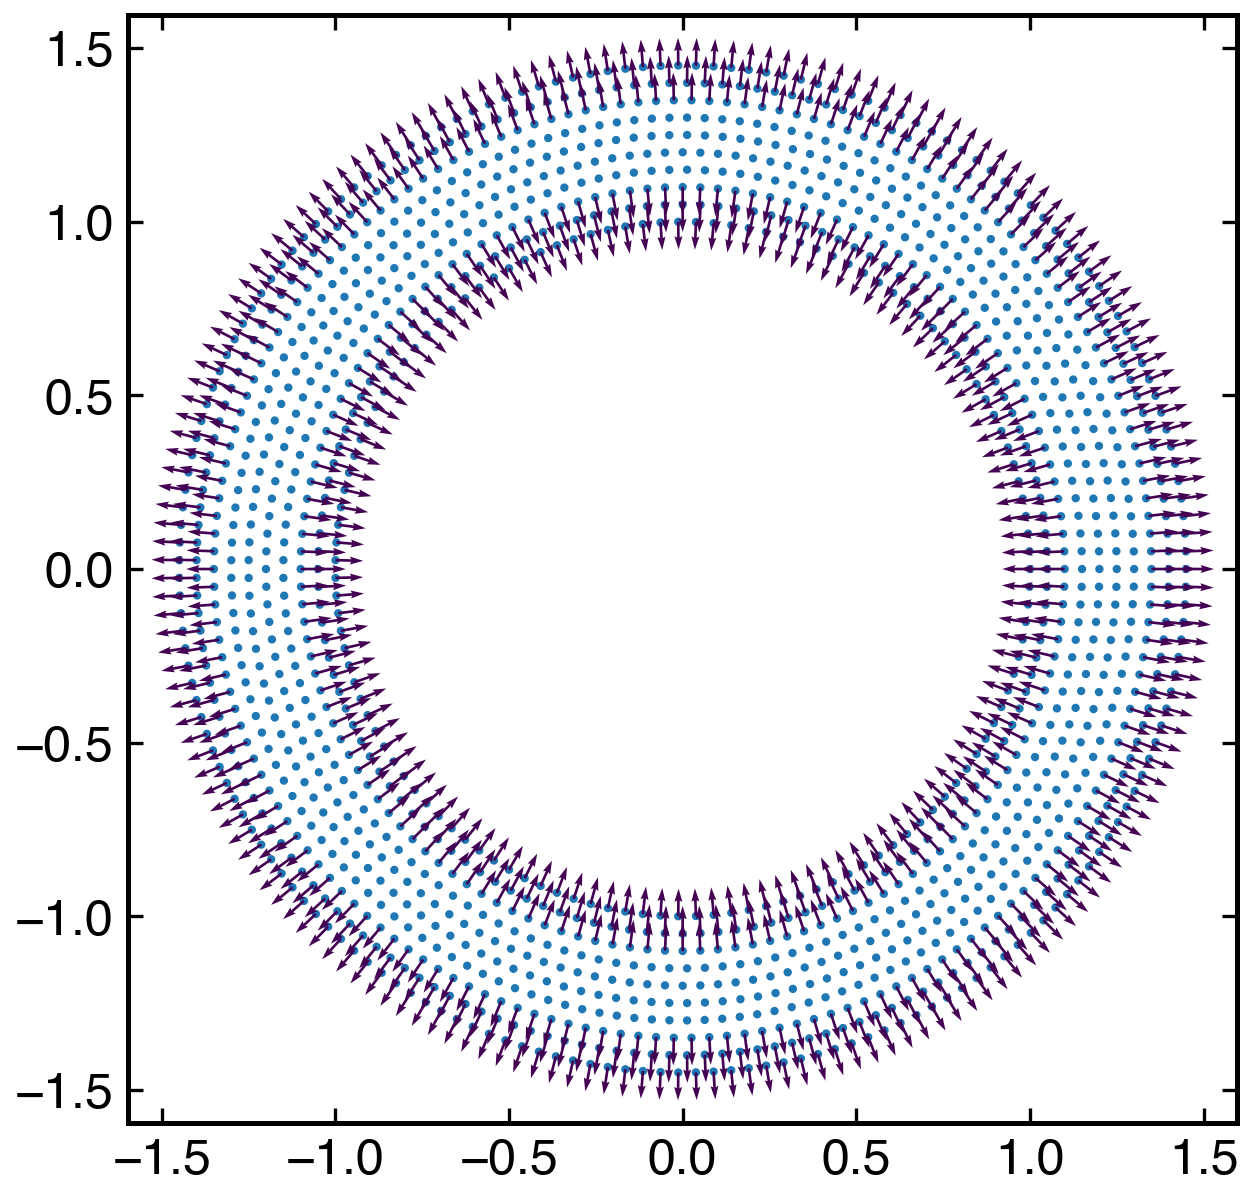
\includegraphics[width=1\linewidth]{figures/ctvf/figures/free_surface_identification_demonstration/circle_geometry_normals}
    \subcaption{}%
    \label{fig:free_surface_circle_normals}
  \end{subfigure}
%%%
  \begin{subfigure}{0.48\textwidth}
    \centering
    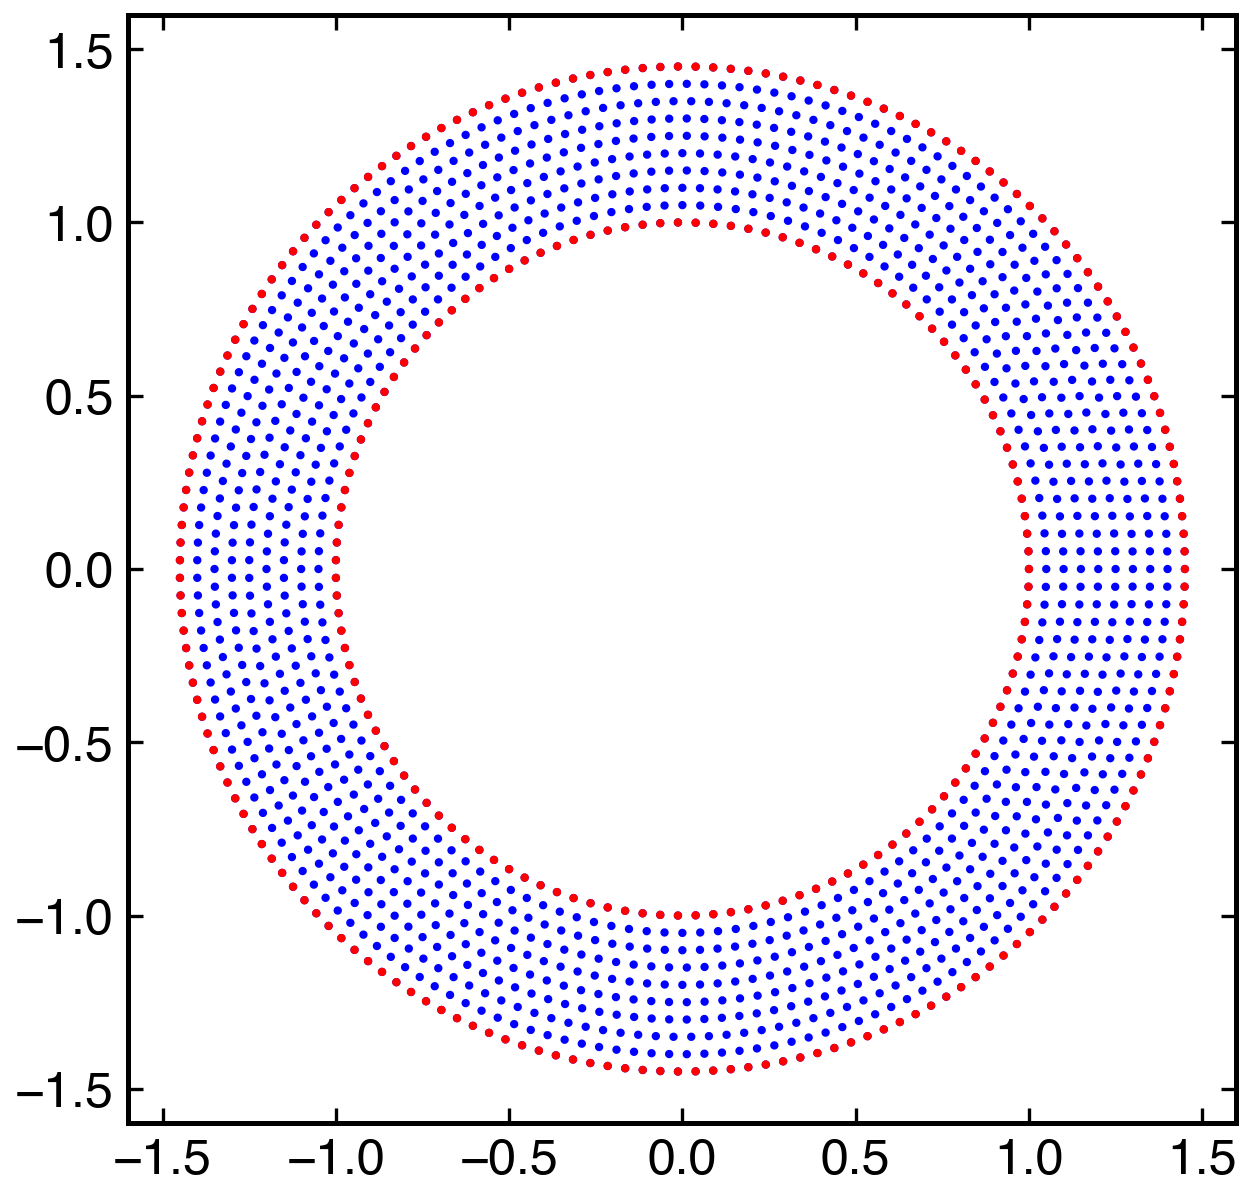
\includegraphics[width=1\linewidth]{figures/ctvf/figures/free_surface_identification_demonstration/circle_geometry}
    \subcaption{}%
    \label{fig:free_surface_circle_boundary_particles}
  \end{subfigure}
  \caption{Identification of free surface particles of a circular ring of
    fluid. Depicts (a) normals of the fluid particles, (b) boundary particles
    of the fluid particles}
\label{fig:boundary-particles-circle}
\end{figure}
%%%
%%%
%%%
\begin{figure}
  \centering
  \begin{subfigure}{0.48\textwidth}
    \centering
    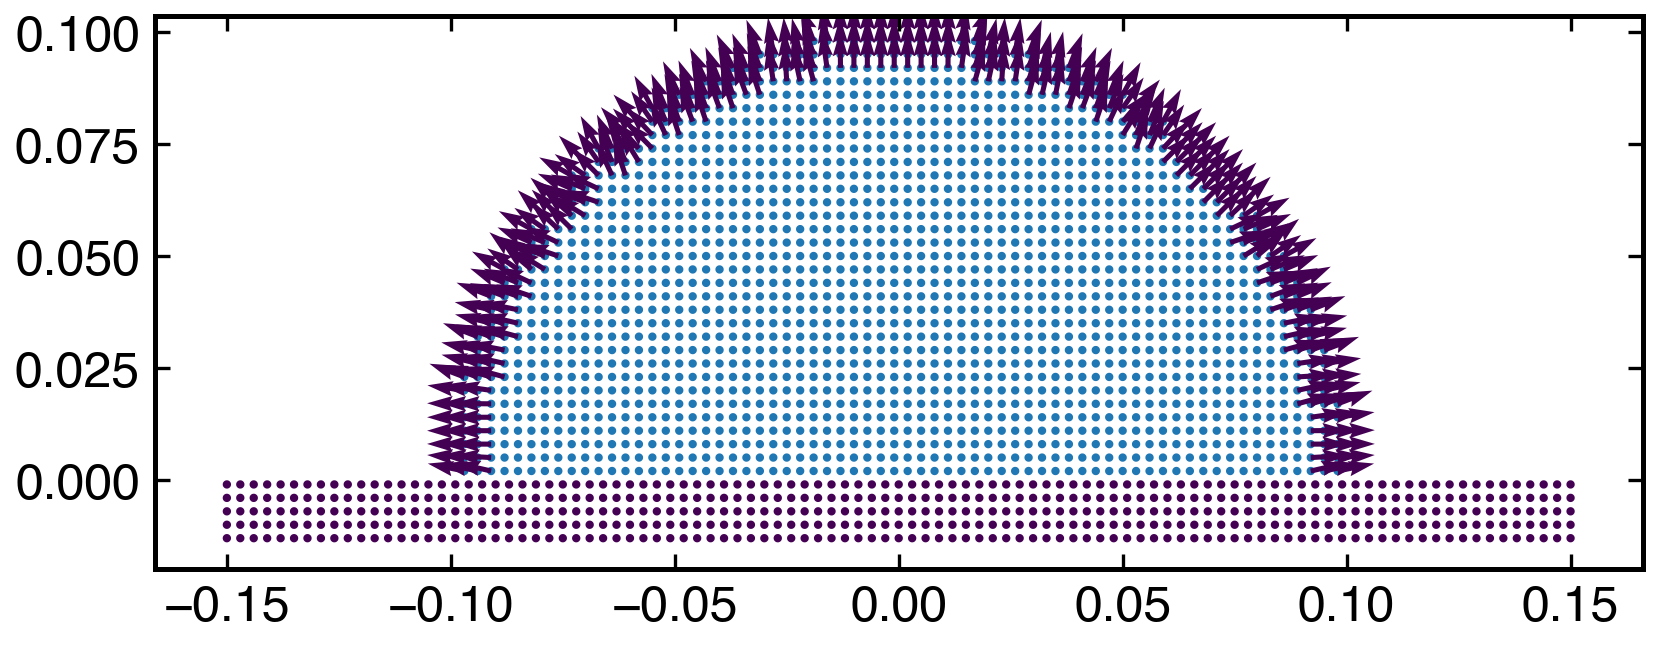
\includegraphics[width=1\linewidth]{figures/ctvf/figures/free_surface_identification_demonstration/circle_with_boundary_normals}
    \subcaption{}%
    \label{fig:boundary-particles-circle-wall-normals}
  \end{subfigure}
%%%
  \begin{subfigure}{0.48\textwidth}
    \centering
    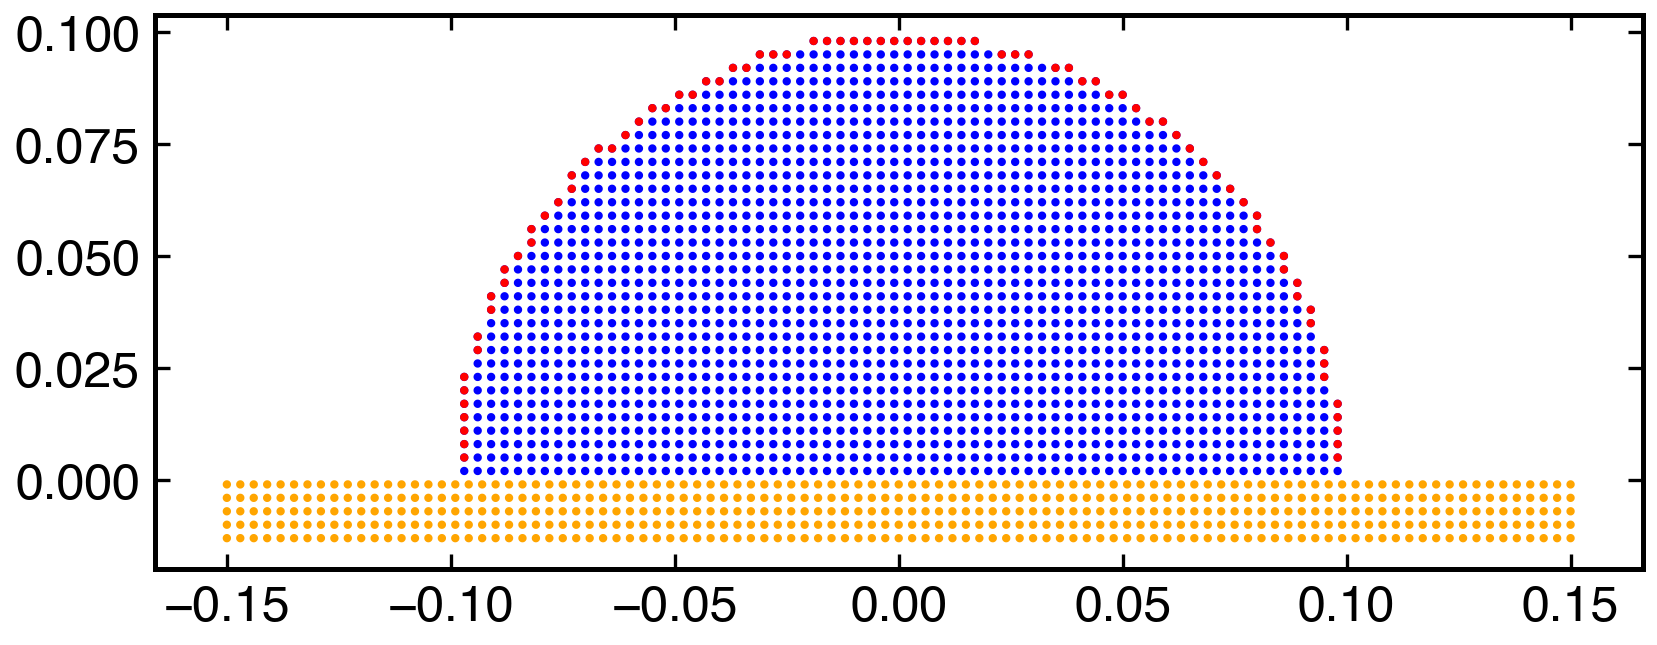
\includegraphics[width=1\linewidth]{figures/ctvf/figures/free_surface_identification_demonstration/circle_with_boundary}
    \subcaption{}%
    \label{fig:boundary-particles-circle-wall-bp}
  \end{subfigure}
  \caption{Identification of free surface particles of a fluid resting on a
    wall. Depicts (a) normals of the fluid particles, (b) boundary particles
    of the fluid particles}
\label{fig:boundary-particles-circle-wall}
\end{figure}
%%%
%%%
%%%
%%%
\begin{figure}
  \centering
  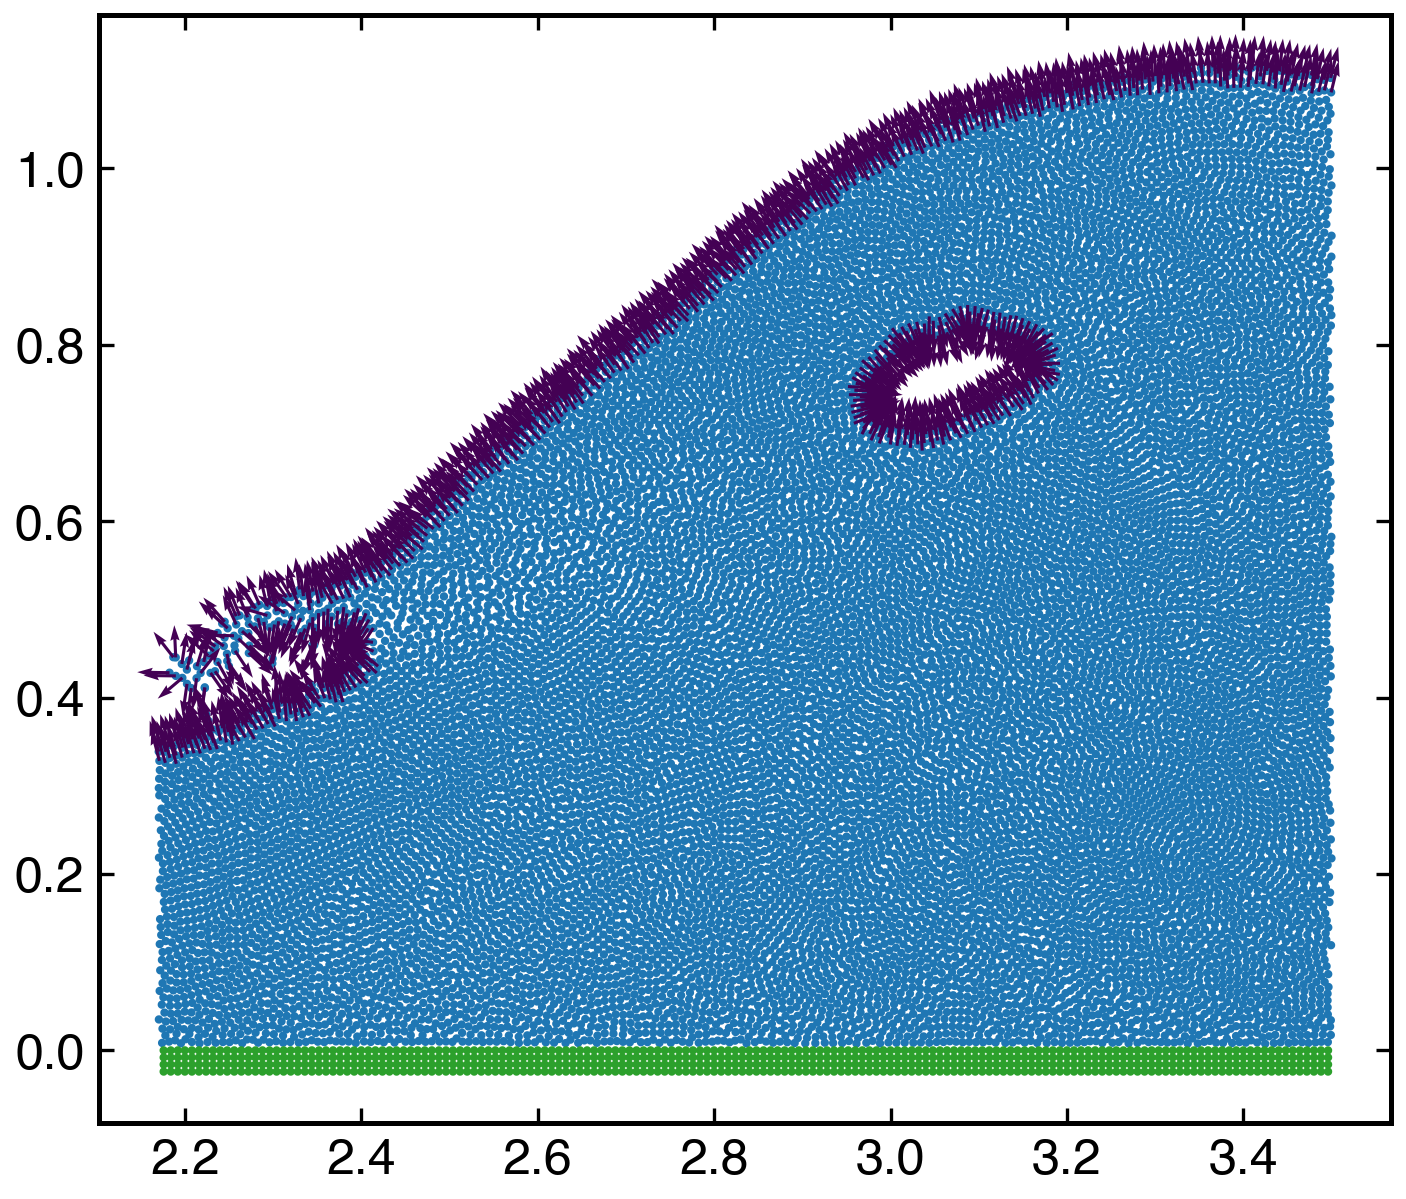
\includegraphics[width=1\linewidth]{figures/ctvf/figures/free_surface_identification_demonstration/normals_dam_break_final_zoomed}
  \caption{Identification of normals of fluid in a dam break simulation. Shows
    us the normals of all the fluid particles}
\label{fig:normals}
\end{figure}


\begin{figure}
  \centering
  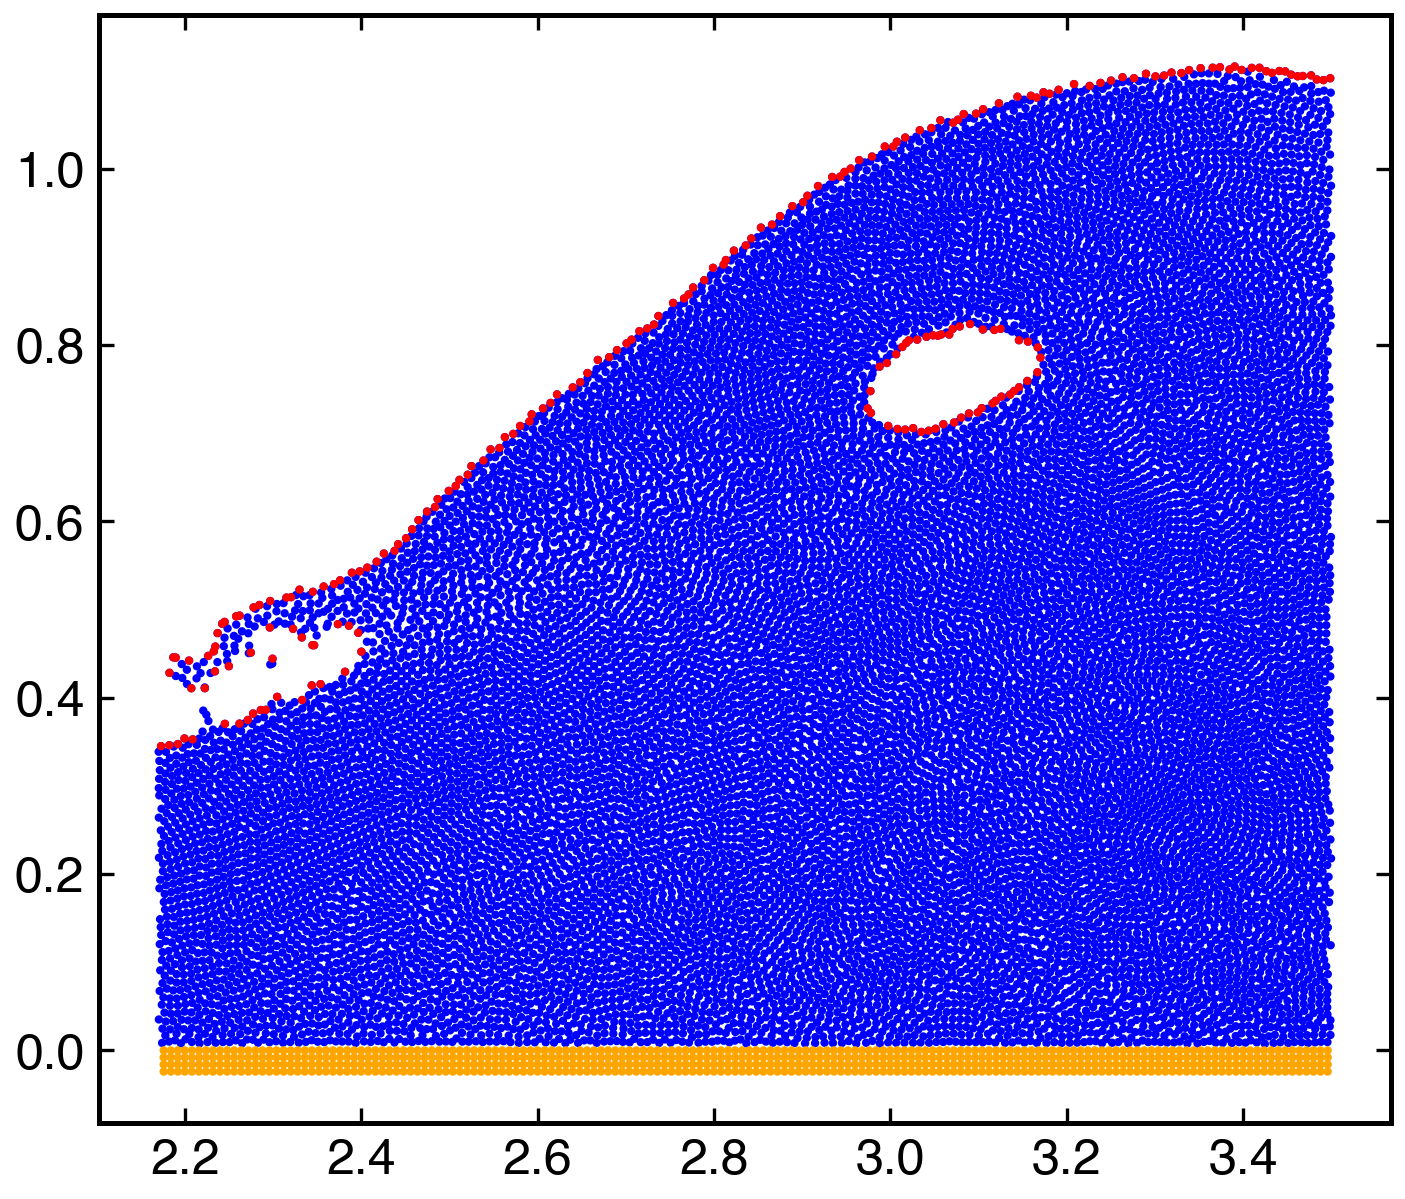
\includegraphics[width=1\linewidth]{figures/ctvf/figures/free_surface_identification_demonstration/boundary_particles_final_zoomed}
  \caption{Identification of boundary particles of fluid at an instance in a
    dam break. Shows boundary particles of all the fluid particles}
\label{fig:boundary-particles}
\end{figure}
%
%
%
%
\subsection{PST Close to the Free Surface}
\label{sec:pst-free-surf}

Near the free-surface the PST has to be performed with some care for both
fluids and solids. This is because of the lack of support for the particles
near the free-surface. After the free surface particles are identified by
using the algorithm described in \cref{subsec:free-surface}, we mark the
particles which are in close proximity to the free surface particles. This is
done through a variable associated with each particle called $h_{b}$, which is
initialized to the initial smoothing length of the particles.

We loop over all the particles that are not on the boundary, and their $h_b$
is adjusted to the distance to the closest boundary particle divided
appropriately by a kernel-dependent factor such that the kernel support is up
to the closest boundary particle. In the current work, we have used a quintic
spline kernel for which the factor is 3. The algorithm is shown in
\cref{alg:hb} and depicted in \cref{fig:pst_free_surf}. We note that this
$h_b$ is only used for the PST force/displacement computation. This process
allows us to ensure that the homogenization force does not push these
particles towards the free-surface.
%
\begin{algorithm}[!ht]
  \caption{Algorithm to set $h_b$}%
  \label{alg:hb}
  \begin{algorithmic}[1]
    \For{particle $i$ in all particles}
    \If{$i$ is a boundary particle}
    \State{set $h_{b, i} = 0$}
    \Else
    \State{set $h_{b,i} = h$}
    \EndIf
    \EndFor%
    \For{particle $i$ in all non-boundary particles}
    \If{particle $i$ has a boundary particle in its neighborhood}
     \State{$x_{\text{dist}, i} \leftarrow$ Distance to nearest boundary
       particle}
     \State{Set $h_{b,i} = \frac{x_{\text{dist, i}}}{3}$}
    \EndIf
    \EndFor%
  \end{algorithmic}
\end{algorithm}
%


\begin{figure}
  \centering
  \begin{subfigure}{0.3\textwidth}
    \centering
    \includegraphics[width=1\linewidth]{images/ctvf/images/pst_free_surf/pst_free_surface}
    \subcaption{}%
    \label{fig:pst_free_surf}
  \end{subfigure}
%
  \begin{subfigure}{0.1\textwidth}
    \centering
    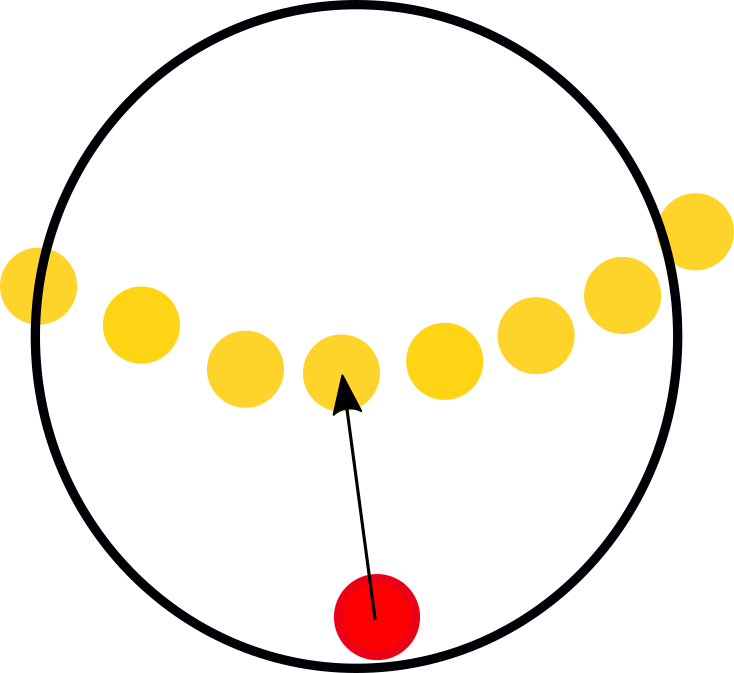
\includegraphics[width=1\linewidth]{images/ctvf/images/pst_free_surf/pst_free_surface_zoomed}
    \subcaption{}%
    \label{fig:pst_free_surf_zoomed}
  \end{subfigure}
  \caption{
    Set $h_b$ of the particles. (a) Particles with a free surface whose
    free particles are identified (b) Minimum distance between the particle in
    the vicinity of the free surface to the free surface particle.}
\label{fig:pst_free_surf}
\end{figure}
%


In the PST of \cite{sun_consistent_2019}, the shifting acceleration is
adjusted using
\begin{equation}
 \label{eq:shifting_force_free_surface_adjust_sun2019}
 \bigg(\frac{d \ten{u}_a}{dt}\bigg)_{\text{c}} =\begin{cases}
   0& \text{if boundary},\\
   \big(\frac{d \ten{u}_a}{dt}\big)_{\text{c}}  - (\big(\frac{d \ten{u}_a}{dt}\big)_{\text{c}} \cdot \ten{n}_a) \ten{n}_a& \text{if $h_b < h$},\\
   \big(\frac{d \ten{u}_a}{dt}\big)_{\text{c}}& \text{if $h_b = h$}.
 \end{cases}
\end{equation}
Whereas while using IPST~\citep{huang_kernel_2019}, rather than adjusting the
final shifting acceleration, we adjust the increment in the position of
\cref{eq:ipst_step2},
\begin{equation}
 \label{eq:shifting_force_free_surface_adjust_ipst}
 \delta \ten{r}_a^{m} =\begin{cases}
   0& \text{if boundary},\\
   \delta \ten{r}_a^{m} - (\delta \ten{r}_a^{m}  \cdot \ten{n}_a) \ten{n}_a& \text{if $h_b < h$},\\
   \delta \ten{r}_a^{m}& \text{if $h_b = h$}.
 \end{cases}
\end{equation}

\subsection{Boundary Conditions}

The ghost particle approach of \cite{Adami2012} is used to model the
boundaries. We use three layers of ghost particles to model the solid wall.
The properties of the solid wall are interpolated from the fluid particles.

When computing the divergence of the velocity field on fluid particles, we
enforce a no-penetration boundary condition and not a no-slip boundary
condition. The velocity of the fluid is projected onto the ghost particles
using,
\begin{equation}
  \label{eq:v-ghost}
  \ten{\hat{u}}_a = \frac{\sum_b\ten{u}_b W_{ab}}{\sum_b W_{ab}},
\end{equation}
\begin{equation}
  \label{eq:v-hat-ghost}
  \ten{\check{u}}_a = \frac{\sum_b\tilde{\ten{u}}_b W_{ab}}{\sum_b W_{ab}},
\end{equation}
where $\ten{u}_b$, $\ten{\tilde{u}}_b$ are the momentum and transport velocity
of the fluid respectively and $W_{ab}$ is the kernel value between the fluid
particle and the ghost particle.

The normal component of this projected velocity is then reflected and set as
the ghost particle velocity,
\begin{equation}
  \label{eq:free-slip-bc-u}
  \ten{u}_{\text{Ga}} = 2 \ten{\hat{n}}((\ten{u}_{\text{p}} - \ten{\hat{u}}_{\text{a}})\cdot \ten{\hat{n}}) + \ten{\hat{u}}_{\text{a}},
\end{equation}
where $\ten{u}_{\text{p}}$ is the local velocity of the boundary and
$\ten{\hat{n}}$ is the unit normal to the boundary particle $a$. Similarly the
transport velocity of the ghost particle is set as,
\begin{equation}
  \label{eq:free-slip-bc-u}
  \tilde{\ten{u}}_{\text{Gi}} = 2 \ten{\hat{n}}((\ten{u}_{\text{p}} - \ten{\check{u}}_{\text{i}})\cdot \ten{\hat{n}}) + \ten{\check{u}}_{\text{i}},
\end{equation}

When the viscous force is computed, the no slip boundary condition is used,
where the velocity on the boundary set as,
\begin{equation}
  \label{eq:no-slip-bc-u}
  \ten{u}_{\text{Ga}} = 2 \ten{u}_{\text{p}} - \ten{\hat{u}}_{\text{a}},
\end{equation}
a similar form is used for the transport velocity here too,
\begin{equation}
  \label{eq:no-slip-bc-uhat}
  \tilde{\ten{u}}_{\text{Ga}} = 2 \ten{u}_{\text{p}} - \ten{\check{u}}_{\text{a}}.
\end{equation}

The pressure of the boundary particle is extrapolated from its surrounding
fluid particles by the following equation,
\begin{equation}
  \label{eq:pressure-bc}
  p_w = \frac{\Sigma_f p_f W_{wf} + (\ten{g} - \ten{a}_{\ten{w}}) \cdot \Sigma_f
    \rho_f \ten{r}_{wf} W_{wf}}{\Sigma_f W_{wf}},
\end{equation}
where $\ten{a}_w$ is the acceleration of the wall. The subscript $f$ denotes
the fluid particles and $w$ denotes the wall particles.

For solid mechanics problems, in addition to the extrapolation of pressure, we
also extrapolate the deviatoric shear stress on to the boundary particles
using,
\begin{equation}
  \label{eq:shear-stress-bc}
  \sigma_{ij}^{'} = \frac{\Sigma_s \sigma_{ij}^{'} \; W_{ws}}{\Sigma_s W_{ws}},
\end{equation}
where $s$ denotes the solid particles.



\subsection{Time Integration}

We use the kick-drift-kick scheme for the time integration. We first move the
velocities of the particles to half time step,
\begin{equation}
  \label{eq:velocity-update-stage-1}
  \ten{u}_a^{n+\frac{1}{2}} = \ten{u}_a^{n} + \frac{\Delta t}{2} \bigg(\frac{\tilde{d}\ten{u}_{a}}{dt}\bigg)^n,
\end{equation}

\begin{equation}
  \label{eq:velocity-hat-update-stage-1}
  \ten{\tilde{u}}_a^{n+\frac{1}{2}} = \ten{u}_a^{n+\frac{1}{2}} + \frac{\Delta t}{2} \bigg(\frac{d\ten{u}_{a}}{dt}\bigg)^{n}_{c}.
\end{equation}
%
Then the time derivatives of density and deviatoric stresses are calculated
using the \cref{eq:sph-discretization-continuity} and
\cref{eq:jaumann-stress-rate}. The new time step density, deviatoric stresses
and particle position are updated by,
\begin{equation}
  \label{eq:density-update-stage-2}
  \rho_{a}^{n+1} = \rho_{a}^{n} + \Delta t \; \bigg(\frac{\tilde{d}\rho_{a}}{dt}\bigg)^{n+\frac{1}{2}},
\end{equation}

\begin{equation}
  \label{eq:pressure-update-stage-2}
  p_{a}^{n+1} = p_{a}^{n} + \Delta t \; \bigg(\frac{\tilde{d}p_{a}}{dt}\bigg)^{n+\frac{1}{2}},
\end{equation}

\begin{equation}
  \label{eq:stress-update-stage-2}
  \teng{\sigma}_{a}^{' \; n+1} = \teng{\sigma}_{a}^{' \; n} +
  \Delta t \; \bigg(\frac{\tilde{d}\teng{\sigma}^{'}_{a}}{dt}\bigg)^{n+\frac{1}{2}},
\end{equation}

\begin{equation}
  \label{eq:position-update-stage-2}
  \ten{r}_{a}^{n+1} = \ten{r}_{a}^{n} + \Delta t \; \ten{\tilde{u}}_{a}^{n+1}.
\end{equation}
%
Finally, at new time-step particle position, the momentum velocity is updated

\begin{equation}
  \label{eq:velocity-update-stage-3}
  \ten{u}_a^{n+1} = \ten{u}_a^{n+\frac{1}{2}} + \frac{\Delta t}{2} \bigg(\frac{\tilde{d}\ten{u}_{a}}{dt}\bigg)^{n+1}.
\end{equation}


For the numerical stability, the time step depends on the CFL condition as,
\begin{equation}
  \label{eq:time-step-cfl}
  \Delta t = \mathrm{min} \bigg( 0.25 \; \frac{h}{c + |U|} ,  0.25 \; \frac{h^2}{\nu},  0.25 \; \frac{h^2}{g} \bigg),
\end{equation}
where $|U|$ is the maximum velocity magnitude, $c$ is the speed of sound
typically chosen as $10 |U|$ for fluids in this work.

%
For solid mechanics, the timestep is set based on the following,
\begin{equation}
  \label{eq:time-step-body-force}
  \Delta t \leq 0.25 \; \bigg(\frac{h}{c_0 + |U|} \bigg),
\end{equation}
where $c_0$ is the speed of sound of the solid body.

\section{Results}
\label{sec:results}

We validate the proposed scheme using a suite of benchmark problems for both
fluid and solid mechanics. We first consider fluids where we look at the
Taylor-Green vortex problem, the lid-driven cavity, and the two-dimensional
dam-break problem. We then consider problems in elastic dynamics like the
oscillating plate, a uniaxial compression problem, the collision of rubber
rings, and a high-velocity impact problem. We show how the proposed method is an
improvement on previous work. The method is implemented using the PySPH
framework~\citep{PR:pysph:scipy16,pysph2020}. Every result shown is produced
using an automation framework~\citep{pr:automan:2018}. The source code is
available at \url{https://gitlab.com/pypr/ctvf}.

\FloatBarrier%

\subsection{Taylor-Green Vortex}
\label{sec:tgv}

In the first benchmark, we test the accuracy of the correction terms and
evaluate the different particle shifting schemes introduced in the proposed
scheme by simulating a Taylor-Green vortex. It consists of a periodic unit box
with no solid boundaries. Taylor-Green vortex problem has an exact solution
given as,
\begin{align}
  \label{eq:tgv_sol}
  u &= - U e^{bt} \cos(2 \pi x) \sin(2 \pi y) \\
  v &=   U e^{bt}\sin(2 \pi x) \cos(2 \pi y) \\
  p &=  -U^2 e^{2bt} (\cos(4 \pi x) + \cos(4 \pi y))/4,
\end{align}
where $U$ is chosen as $1$ m\,s\textsuperscript{-1}, $b=-8\pi^2/Re$, $Re=U L /\nu$,
and $L=1$ m. We initialize the fluid using this at $t=0$ and compare the
results with the exact solution. The Reynolds number, $Re$, is initially
chosen to be $100$. The quintic spline with $h/\Delta x = 1.0$ is used. We use
summation density to compute the density and evolve pressure with
\cref{eq:sph-discretization-edac}. No artificial viscosity is used for this
problem.
%
%
The decay rate of the velocity is studied using the evolution of maximum
velocity $|\ten{u}_{\max}|$ in time. We compute the $L_1$ error in the
velocity magnitude as,
\begin{equation}
  \label{eq:tg:l1}
  L_1 = \frac{\sum_i |\ten{u}_{i, computed}| - |\ten{u}_{i, exact}|}
  {\sum_i |\ten{u}_{i, exact}|},
\end{equation}
where $\ten{u}_{i, exact}$ is found at the position of the $i$'th particle.


In \cref{fig:tg_sun2019:tg_decay} we compare the decay of $|\ten{u}_{\max}|$
with that of the exact solution for the case where we use SPST for particle
shifting. As can be seen, the results are in excellent agreement with the
expected decay. The same is seen in \cref{fig:tg_ipst:tg_decay} for the case
using IPST. This shows the accuracy and robustness of the scheme with respect
to changing the PST method. \Cref{fig:tg_sun2019:tg_l1} and
\cref{fig:tg_ipst:tg_l1} show the $L_1$ error of velocity magnitude for
various resolutions simulated using the two PST techniques.
\Cref{fig:tg_sun2019_corrections:tg_l1} depicts the $L_1$ error of velocity
magnitude for a Reynolds number of 100 and 1000 using SPST with and without
correction terms. \Cref{fig:tg_ipst_corrections:tg_l1} shows the same but
using the IPST. The improvement due to the correction terms is clearly seen
as a significant reduction in the error.


One can see that the IPST has lower errors at initial times. However,
we do note that there appears to be a lack of convergence in the result as the
resolution is increased. As the number of particles is increased the $L_1$
error does not correspondingly reduce. This is due to the low Reynolds number
and the discretization of the viscous term that is being used. We show the
results of the velocity decay and the $L_1$ error when a Reynolds number of
1000 is used in \cref{fig:tg_re_1000:ipst} for IPST and in
\cref{fig:tg_re_1000:sun2019} with SPST. In this case the convergence
is clearly seen as the resolution is increased. \Cref{fig:tg_re_1000:pplot}
shows distribution of particles with the color representing pressure. The
Reynolds number of 1000 with a resolution of 150$\times$150. We can see
that the pressure distribution is smooth.

\begin{figure}
  \centering
  \begin{subfigure}{0.48\textwidth}
    \centering
    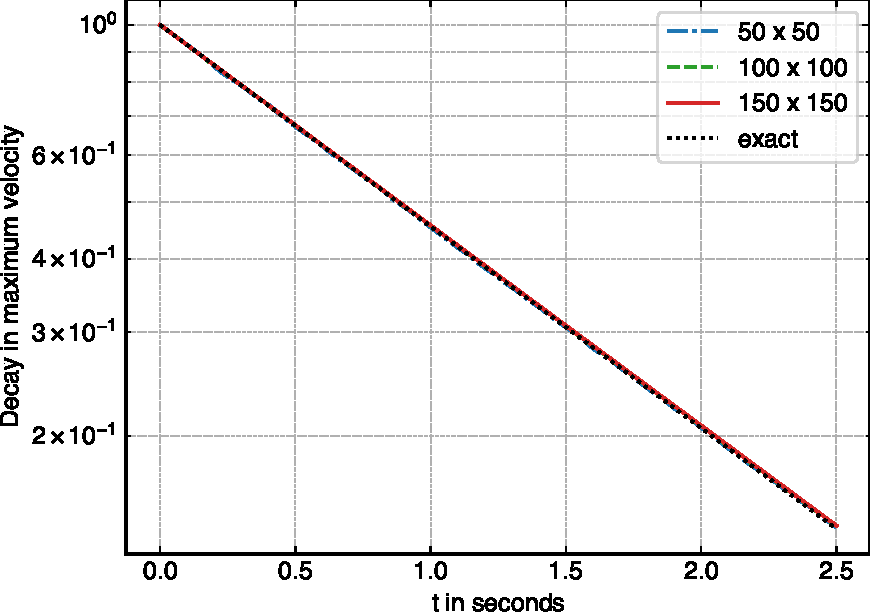
\includegraphics[width=1\linewidth]{figures/ctvf/figures/taylor_green/tg_decay}
    \subcaption{}%
    \label{fig:tg_sun2019:tg_decay}
  \end{subfigure}
%
  \begin{subfigure}{0.48\textwidth}
    \centering
    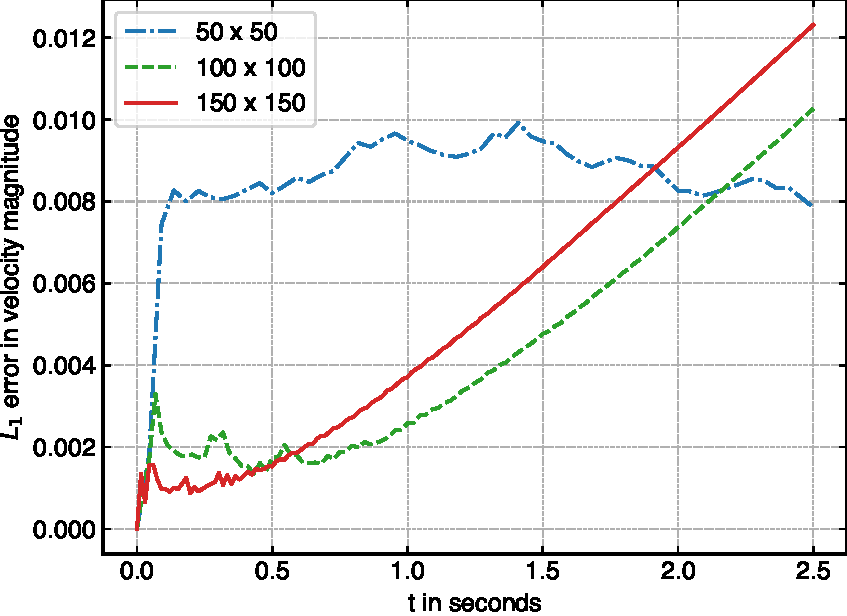
\includegraphics[width=1\linewidth]{figures/ctvf/figures/taylor_green/tg_l1}
    \subcaption{}%
    \label{fig:tg_sun2019:tg_l1}
  \end{subfigure}
  \caption{Taylor-Green vortices for an initial particle distribution of
    $50\times50$, $100\times100$ and $150\times150$ is simulated with a
    Reynolds number of 100 using SPST. Plots shown are (a) decay
    in maximum velocity (b) $L_1$ error in velocity magnitude.}
\label{fig:tg:sun2019}
\end{figure}
%
%
%
\begin{figure}
  \centering
  \begin{subfigure}{0.48\textwidth}
    \centering
    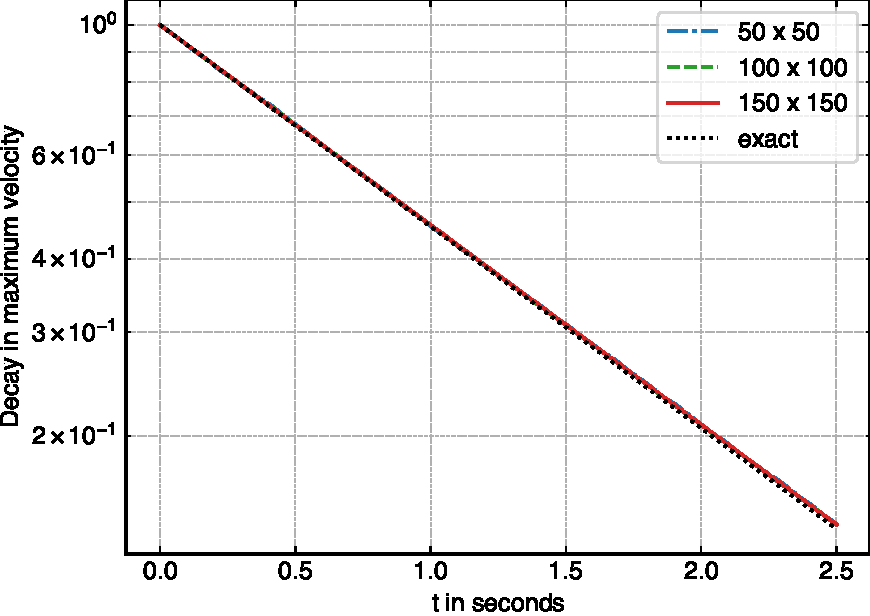
\includegraphics[width=1\linewidth]{figures/ctvf/figures/taylor_green/tg_decay_ipst}
    \subcaption{}%
    \label{fig:tg_ipst:tg_decay}
  \end{subfigure}
%
  \begin{subfigure}{0.48\textwidth}
    \centering
    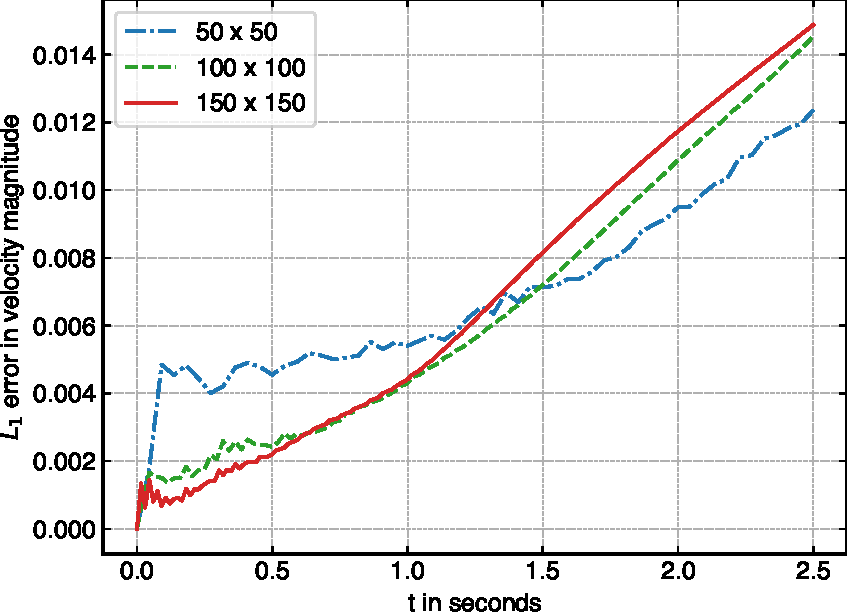
\includegraphics[width=1\linewidth]{figures/ctvf/figures/taylor_green/tg_l1_ipst}
    \subcaption{}%
    \label{fig:tg_ipst:tg_l1}
  \end{subfigure}
  \caption{Taylor-Green vortices for an initial particle distribution of
    $50\times50$, $100\times100$ and $150\times150$ is simulated with a
    Reynolds number of 100 using IPST. Plots shown are (a) decay in
    maximum velocity (b) $L_1$ error in velocity magnitude.}
\label{fig:tg:ipst}
\end{figure}
%
%
\begin{figure}
  \centering
  \begin{subfigure}{0.48\textwidth}
    \centering
    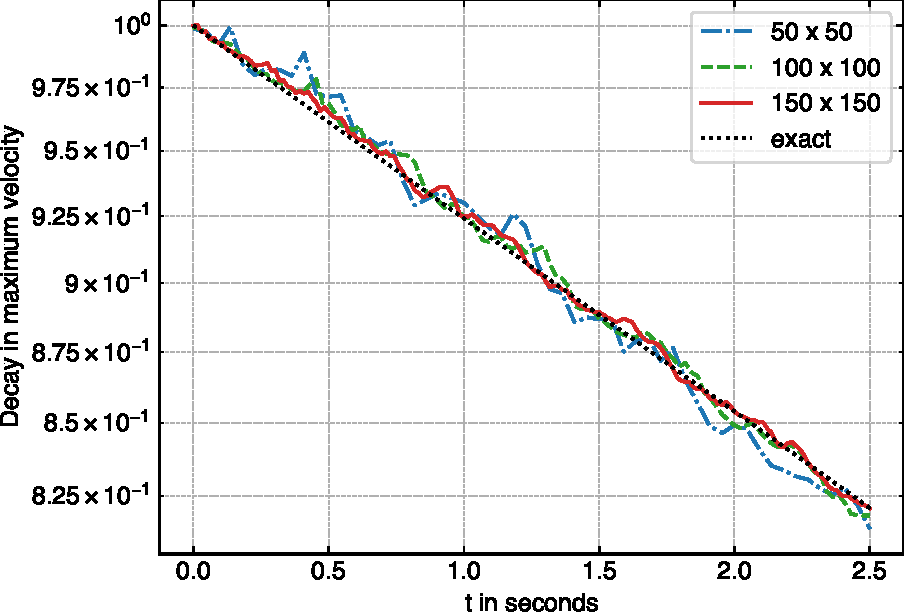
\includegraphics[width=1\linewidth]{figures/ctvf/figures/taylor_green_re_1000/tg_decay_ipst}
    \subcaption{}%
    \label{fig:tg_re_1000_ipst:tg_decay}
  \end{subfigure}
%
  \begin{subfigure}{0.48\textwidth}
    \centering
    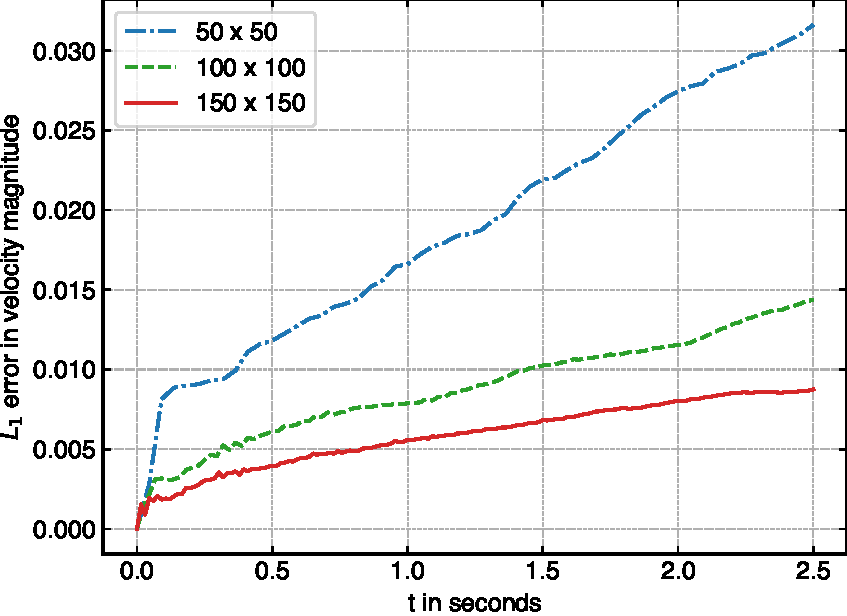
\includegraphics[width=1\linewidth]{figures/ctvf/figures/taylor_green_re_1000/tg_l1_ipst}
    \subcaption{}%
    \label{fig:tg_re_1000_ipst:tg_l1}
  \end{subfigure}
  \caption{Taylor-Green vortices for an initial particle distribution of
    $50\times50$, $100\times100$ and $150\times150$ is simulated with a
    Reynolds number of 1000 using IPST. Plots shown are (a) decay in
    maximum velocity (b) $L_1$ error in velocity magnitude.}
\label{fig:tg_re_1000:ipst}
\end{figure}
%
%
%
\begin{figure}
  \centering
  \begin{subfigure}{0.48\textwidth}
    \centering
    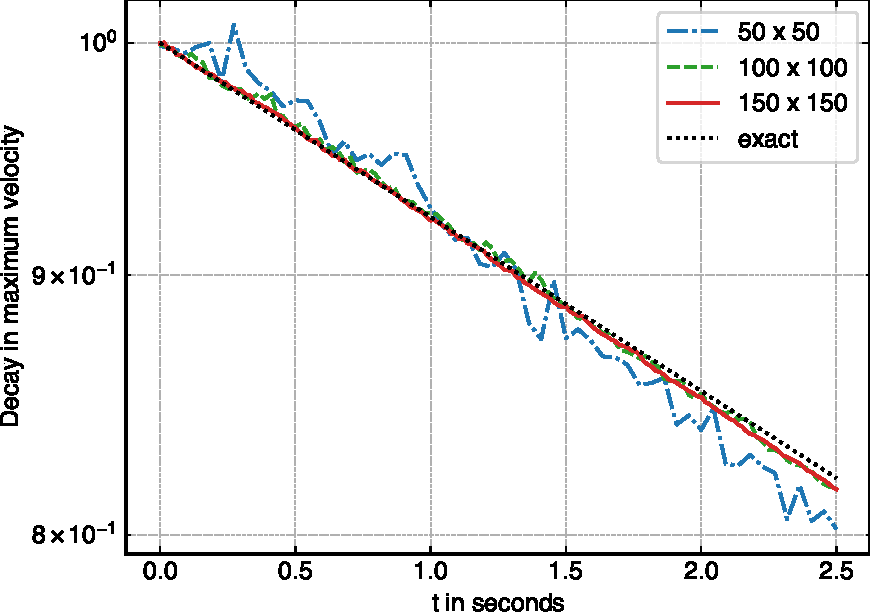
\includegraphics[width=1\linewidth]{figures/ctvf/figures/taylor_green_re_1000/tg_decay}
    \subcaption{}%
    \label{fig:tg_re_1000:tg_decay}
  \end{subfigure}
%
  \begin{subfigure}{0.48\textwidth}
    \centering
    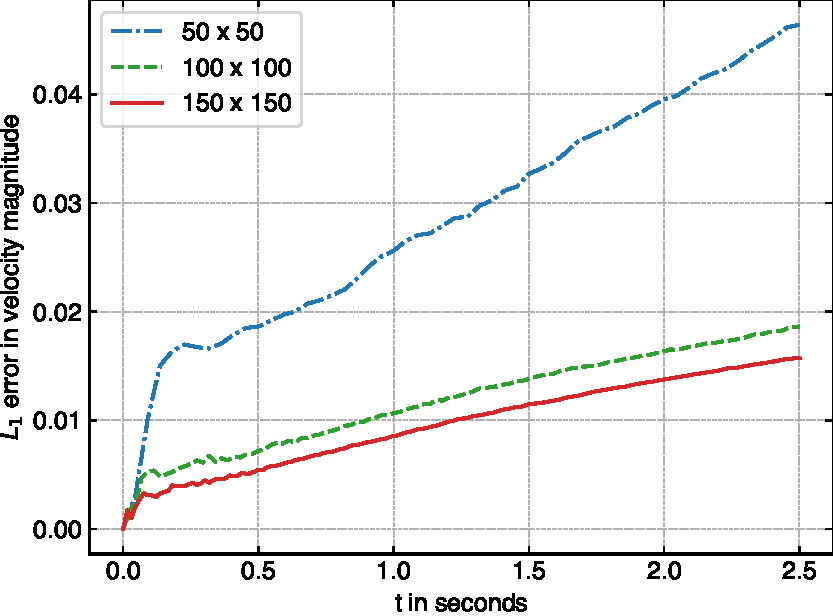
\includegraphics[width=1\linewidth]{figures/ctvf/figures/taylor_green_re_1000/tg_l1}
    \subcaption{}%
    \label{fig:tg_re_1000:tg_l1}
  \end{subfigure}
  \caption{Taylor-Green vortices for an initial particle distribution of
    $50\times50$, $100\times100$ and $150\times150$ is simulated with a
    Reynolds number of 1000 using SPST. Plots shown are (a) decay in
    maximum velocity (b) $L_1$ error in velocity magnitude.}
\label{fig:tg_re_1000:sun2019}
\end{figure}
%
%
%
% comparison plots
\begin{figure}
  \centering
  \begin{subfigure}{0.48\textwidth}
    \centering
    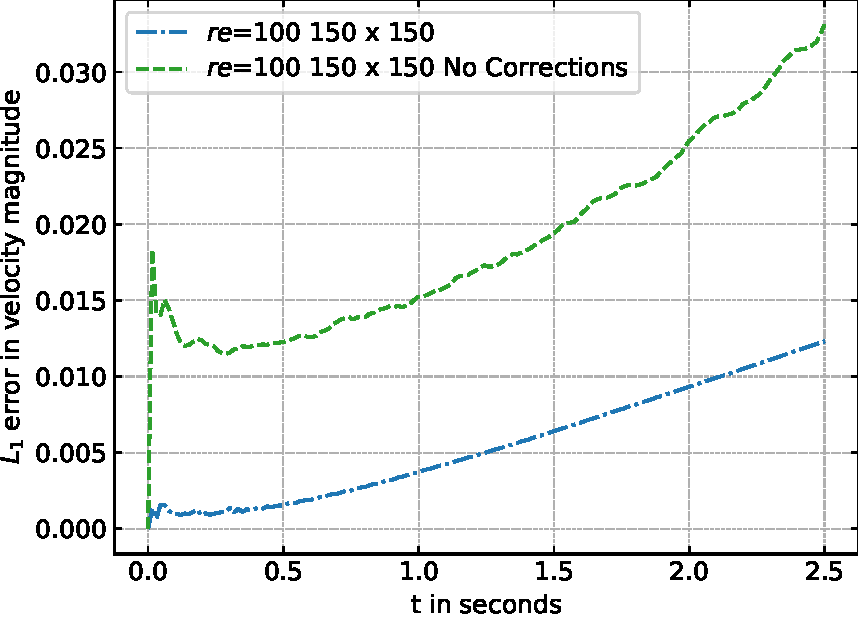
\includegraphics[width=1\linewidth]{figures/ctvf/figures/taylor_green_sun2019_corrections_test/tg_l1_re_100}
    \subcaption{}%
    \label{fig:tg_sun2019_correcions:tg_l1_re_100}
  \end{subfigure}
%
  \begin{subfigure}{0.48\textwidth}
    \centering
    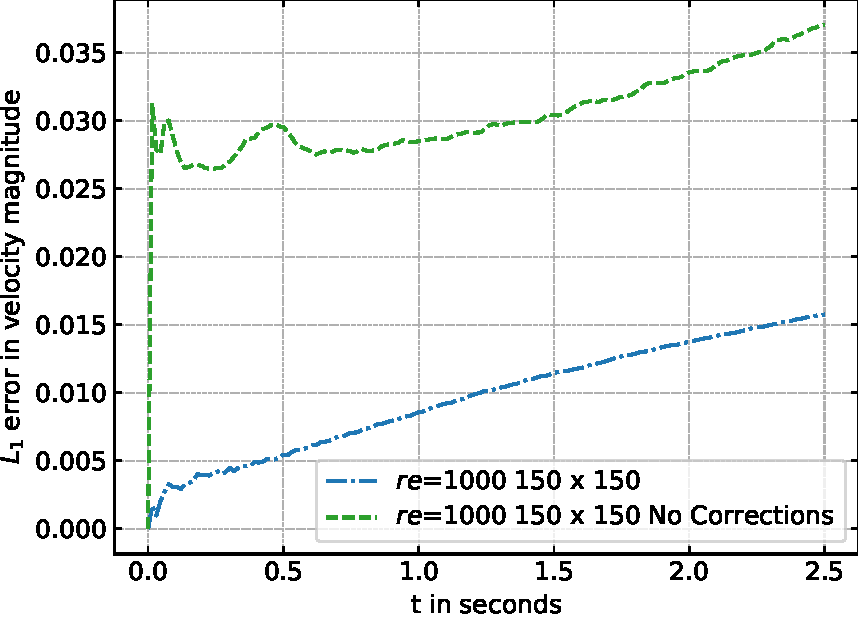
\includegraphics[width=1\linewidth]{figures/ctvf/figures/taylor_green_sun2019_corrections_test/tg_l1_re_1000}
    \subcaption{}%
    \label{fig:tg_sun2019_correcions:tg_l1_re_1000}
  \end{subfigure}
  \caption{$L_1$ error for nx with 150 $\times$ 150 with and without
    corrections with SPST with a Reynolds number of a) 100 and b) 1000}
\label{fig:tg_sun2019_corrections:tg_l1}
\end{figure}
% comparison plots
% comparison plots
\begin{figure}
  \centering
  \begin{subfigure}{0.48\textwidth}
    \centering
    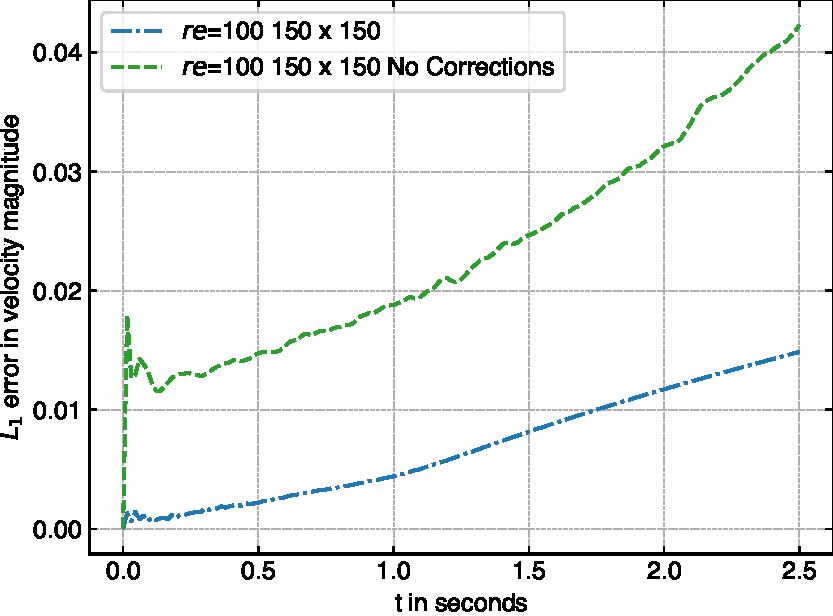
\includegraphics[width=1\linewidth]{figures/ctvf/figures/taylor_green_ipst_corrections_test/tg_l1_re_100}
    \subcaption{}%
    \label{fig:tg_ipst_correcions:tg_l1_re_100}
  \end{subfigure}
%
  \begin{subfigure}{0.48\textwidth}
    \centering
    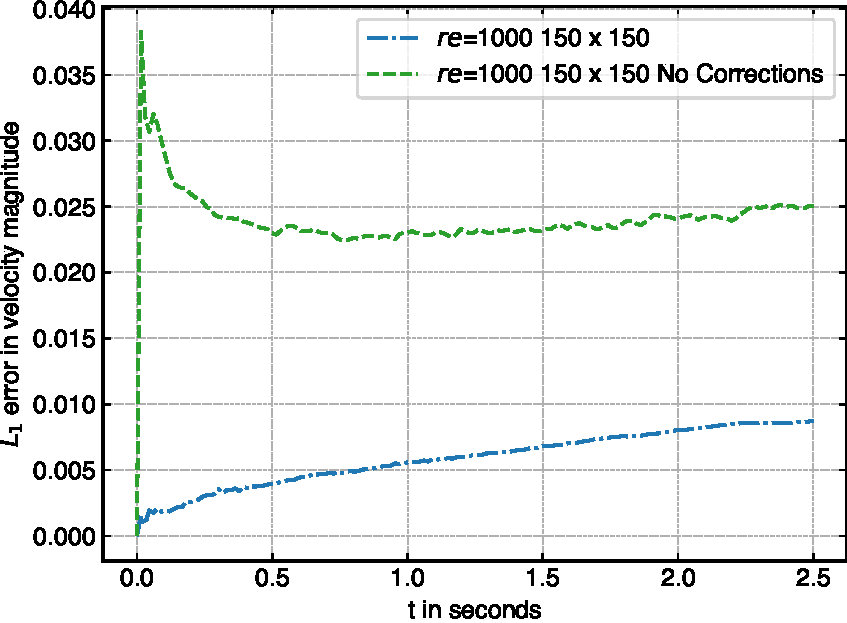
\includegraphics[width=1\linewidth]{figures/ctvf/figures/taylor_green_ipst_corrections_test/tg_l1_re_1000}
    \subcaption{}%
    \label{fig:tg_ipst_correcions:tg_l1_re_1000}
  \end{subfigure}
  \caption{$L_1$ error for nx with 150 $\times$ 150 with and without
    corrections with IPST with a Reynolds number of a) 100 and b)
    1000}
\label{fig:tg_ipst_corrections:tg_l1}
\end{figure}
% comparison plots
%
%

An inspection of figures \ref{fig:tg_sun2019:tg_l1}, \ref{fig:tg_ipst:tg_l1}
and \ref{fig:tg_re_1000_ipst:tg_l1}, \ref{fig:tg_re_1000:tg_l1} suggests that the
IPST  appears to be better than that of SPST.

\begin{figure}
  \centering
  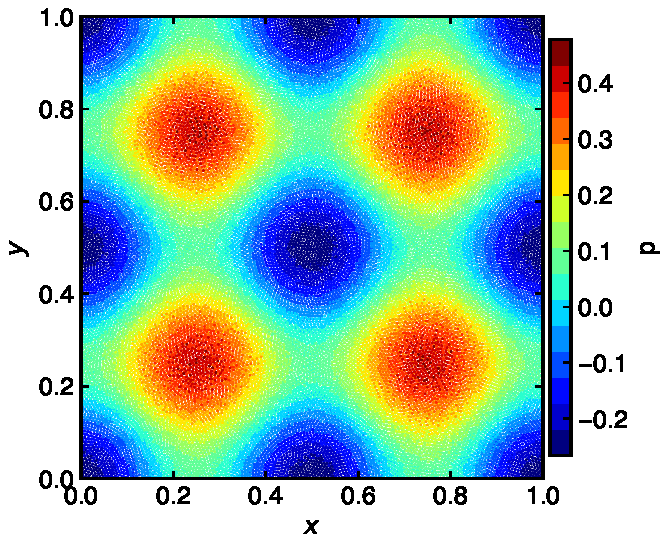
\includegraphics[width=0.5\linewidth]{figures/ctvf/figures/taylor_green_re_1000/tg_pplot_p_re_1000}
  \caption{Particle plot of Taylor green vortices for a Reynolds number of
    1000 with a resolution of $150\times150$. The colors represent the
    pressure.}%
  \label{fig:tg_re_1000:pplot}
\end{figure}
%


\FloatBarrier%
\subsection{Lid Driven Cavity}
\label{sec:ldc}

We evaluate the ability of the proposed scheme to handle solid wall boundary
conditions by simulating a lid-driven cavity. The lid-driven cavity is a
classic problem that can be challenging to simulate in the context of the SPH.
It has been simulated by \citep{Adami2013}, \citep{huang_kernel_2019},
\citep{edac-sph:cf:2019} to note a few. A rectangular cavity with length 1 m
which is filled with fluid is constrained by four walls. Top wall has a
velocity of $U = 1 $ m\,s\textsuperscript{-1}. A unit density is assumed for the
fluid. The speed of sound of the fluid particle is set to $c = 10 U_{max}$. We
use the summation density to compute the density. The viscosity of the fluid
is set through the Reynolds number of the flow, $\nu = \frac{Re}{U}$. No
artificial viscosity is used in the current problem.

%
\begin{figure}
  \centering
  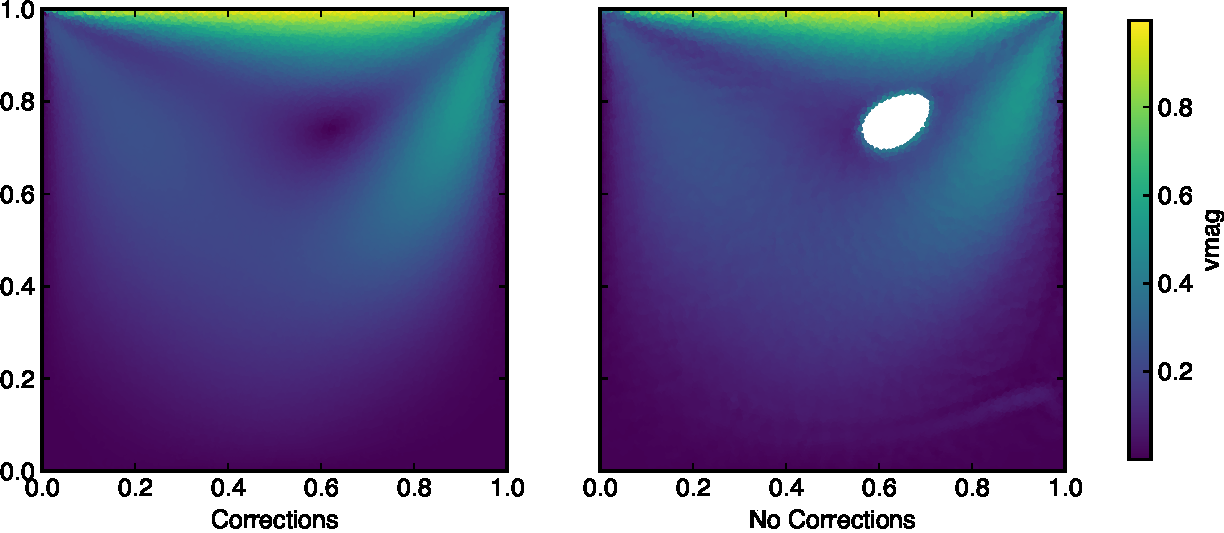
\includegraphics[width=1\linewidth]{figures/ctvf/figures/cavity_sun2019_corrections_test/good_vs_bad}
  \caption{ Particle plot of cavity with a $Re=100$ with particle arrangement
    of $150 \times 150$, left side with corrections and right side without
    correction terms.}%
  \label{fig:ldc:particle_plots_re100_compare}
\end{figure}
%
We first simulate the cavity problem with a Reynolds number of 100 with and
without corrections. In \cref{fig:ldc:particle_plots_re100_compare} we can see
that an unphysical void is produced when no corrections are employed. This is
eliminated with the current scheme.

%
\begin{figure}
  \centering
  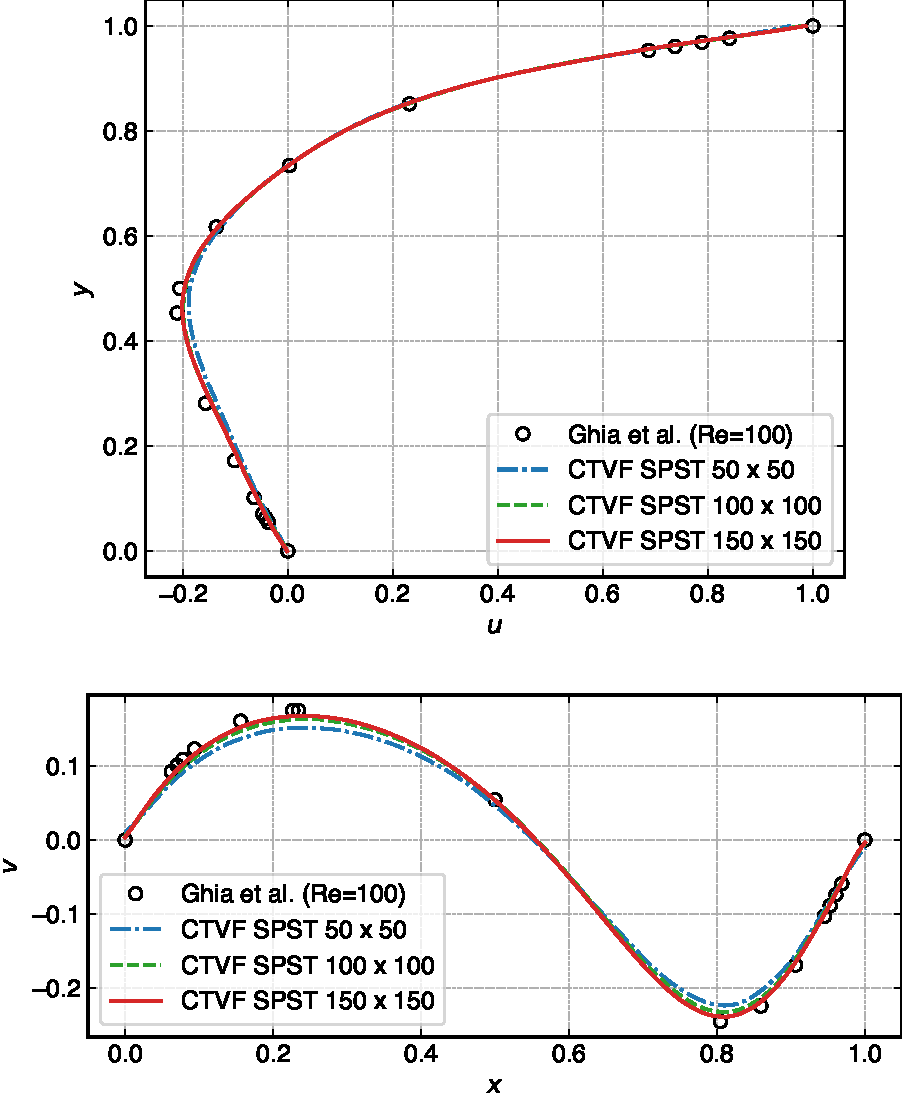
\includegraphics[width=0.5\linewidth]{figures/ctvf/figures/cavity/uv_re100}
  \caption{Velocity profiles $u$ vs.\ $y$ and $v$ vs.\ $x$ for the
    lid-driven-cavity problem at $Re=100$ with three initial particle
    arrangement of $50 \times 50$, $100 \times 100$, and $150 \times
    150$.}%
  \label{fig:ldc:uv_re100}
\end{figure}
%
\begin{figure}
  \centering
  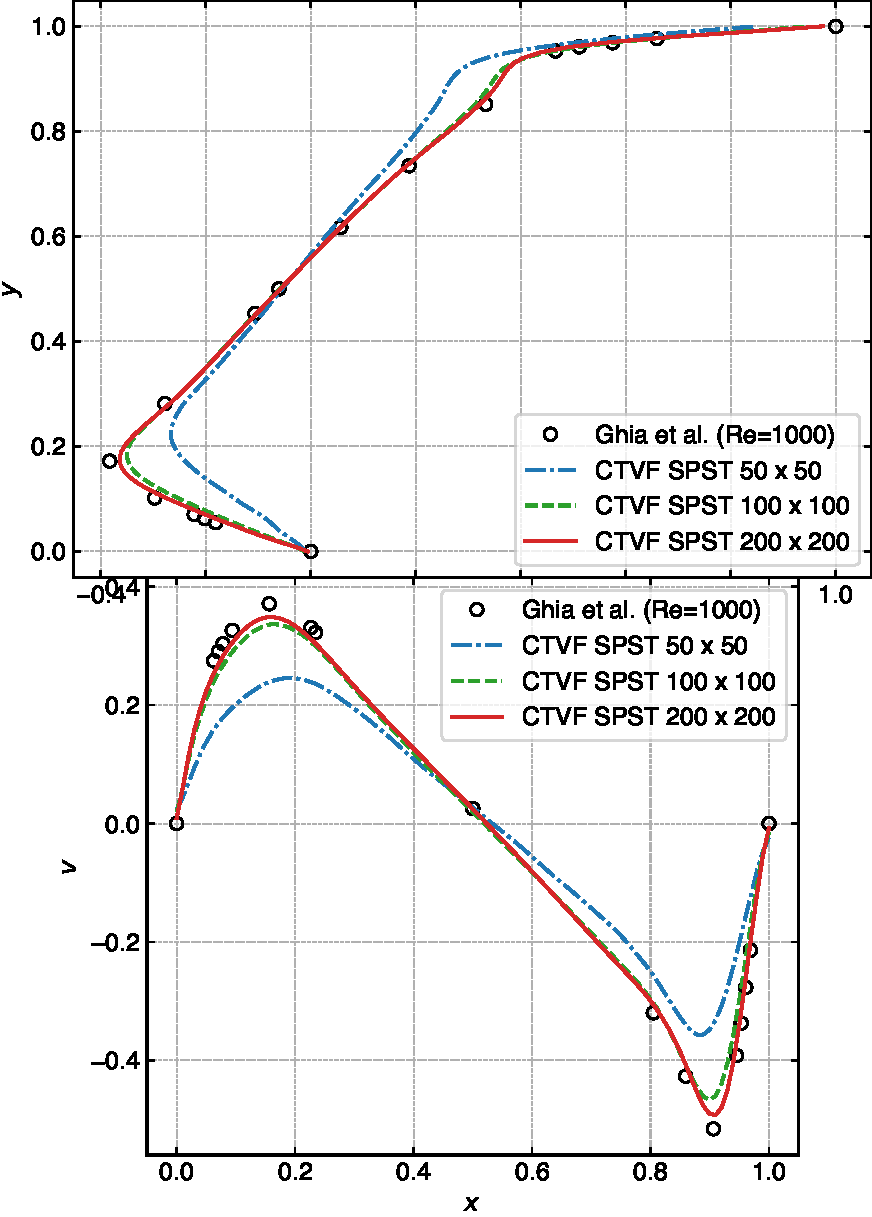
\includegraphics[width=0.5\linewidth]{figures/ctvf/figures/cavity/uv_re1000}
  \caption{Velocity profiles for the lid-driven-cavity using the steady state
    simulation procedure for $Re = 1000$ with initial partial arrangement of
    $50 \times 50$, $100 \times 100$, and $200 \times 200$ compared with
    the results of~\citep{ldc:ghia-1982}.}%
\label{fig:ldc:uv_re1000}
\end{figure}

We now study convergence of the method as we vary the
resolution. \Cref{fig:ldc:uv_re100} and \cref{fig:ldc:uv_re1000} show the
center-line velocities $u$ versus $y$ and $v$ versus $x$ for the Reynolds
numbers 100 and 1000 respectively. For the $Re=100$ case we use three
different resolutions of $50\times 50, 100 \times 100$ and $150 \times
150$. For the $Re=1000$ case, we use an initial $50 \times 50$,
$100 \times 100$, and $200 \times 200$ grid of particles. These are compared
against the results of \citep{ldc:ghia-1982}. As we can see that the current
scheme is able to predict the velocity profiles well.


\FloatBarrier%

\subsection{2D Dam-break}

We apply the proposed scheme to free surface flows by simulating a
dam-break. This problem has been extensively studied before for example in
\citep{muta_efficient_2020}, \citep{zhang_hu_adams17}, and
\citep{edac-sph:cf:2019}.

A block of fluid having width 1m and a height of $2$ m is allowed to settle
under the influence of gravity inside a tank of length $4$ m. The fluid block
is initially placed to the left of the tank. The acceleration due to gravity
is $g=9.81$ m\,s\textsuperscript{-2}. To simulate the free surface flows we
use the continuity equation to evolve the density using
\eqref{eq:sph-discretization-continuity} and the
\eqref{eq:sph-discretization-edac} to evolve the pressure. We use free slip
boundary conditions to compute the divergence of the velocities and a no-slip
boundary condition while computing the viscous forces. The value of
$\alpha=0.05$ is used for the artificial viscosity \cref{eq:mom-av} term.

\begin{figure}
  \centering
  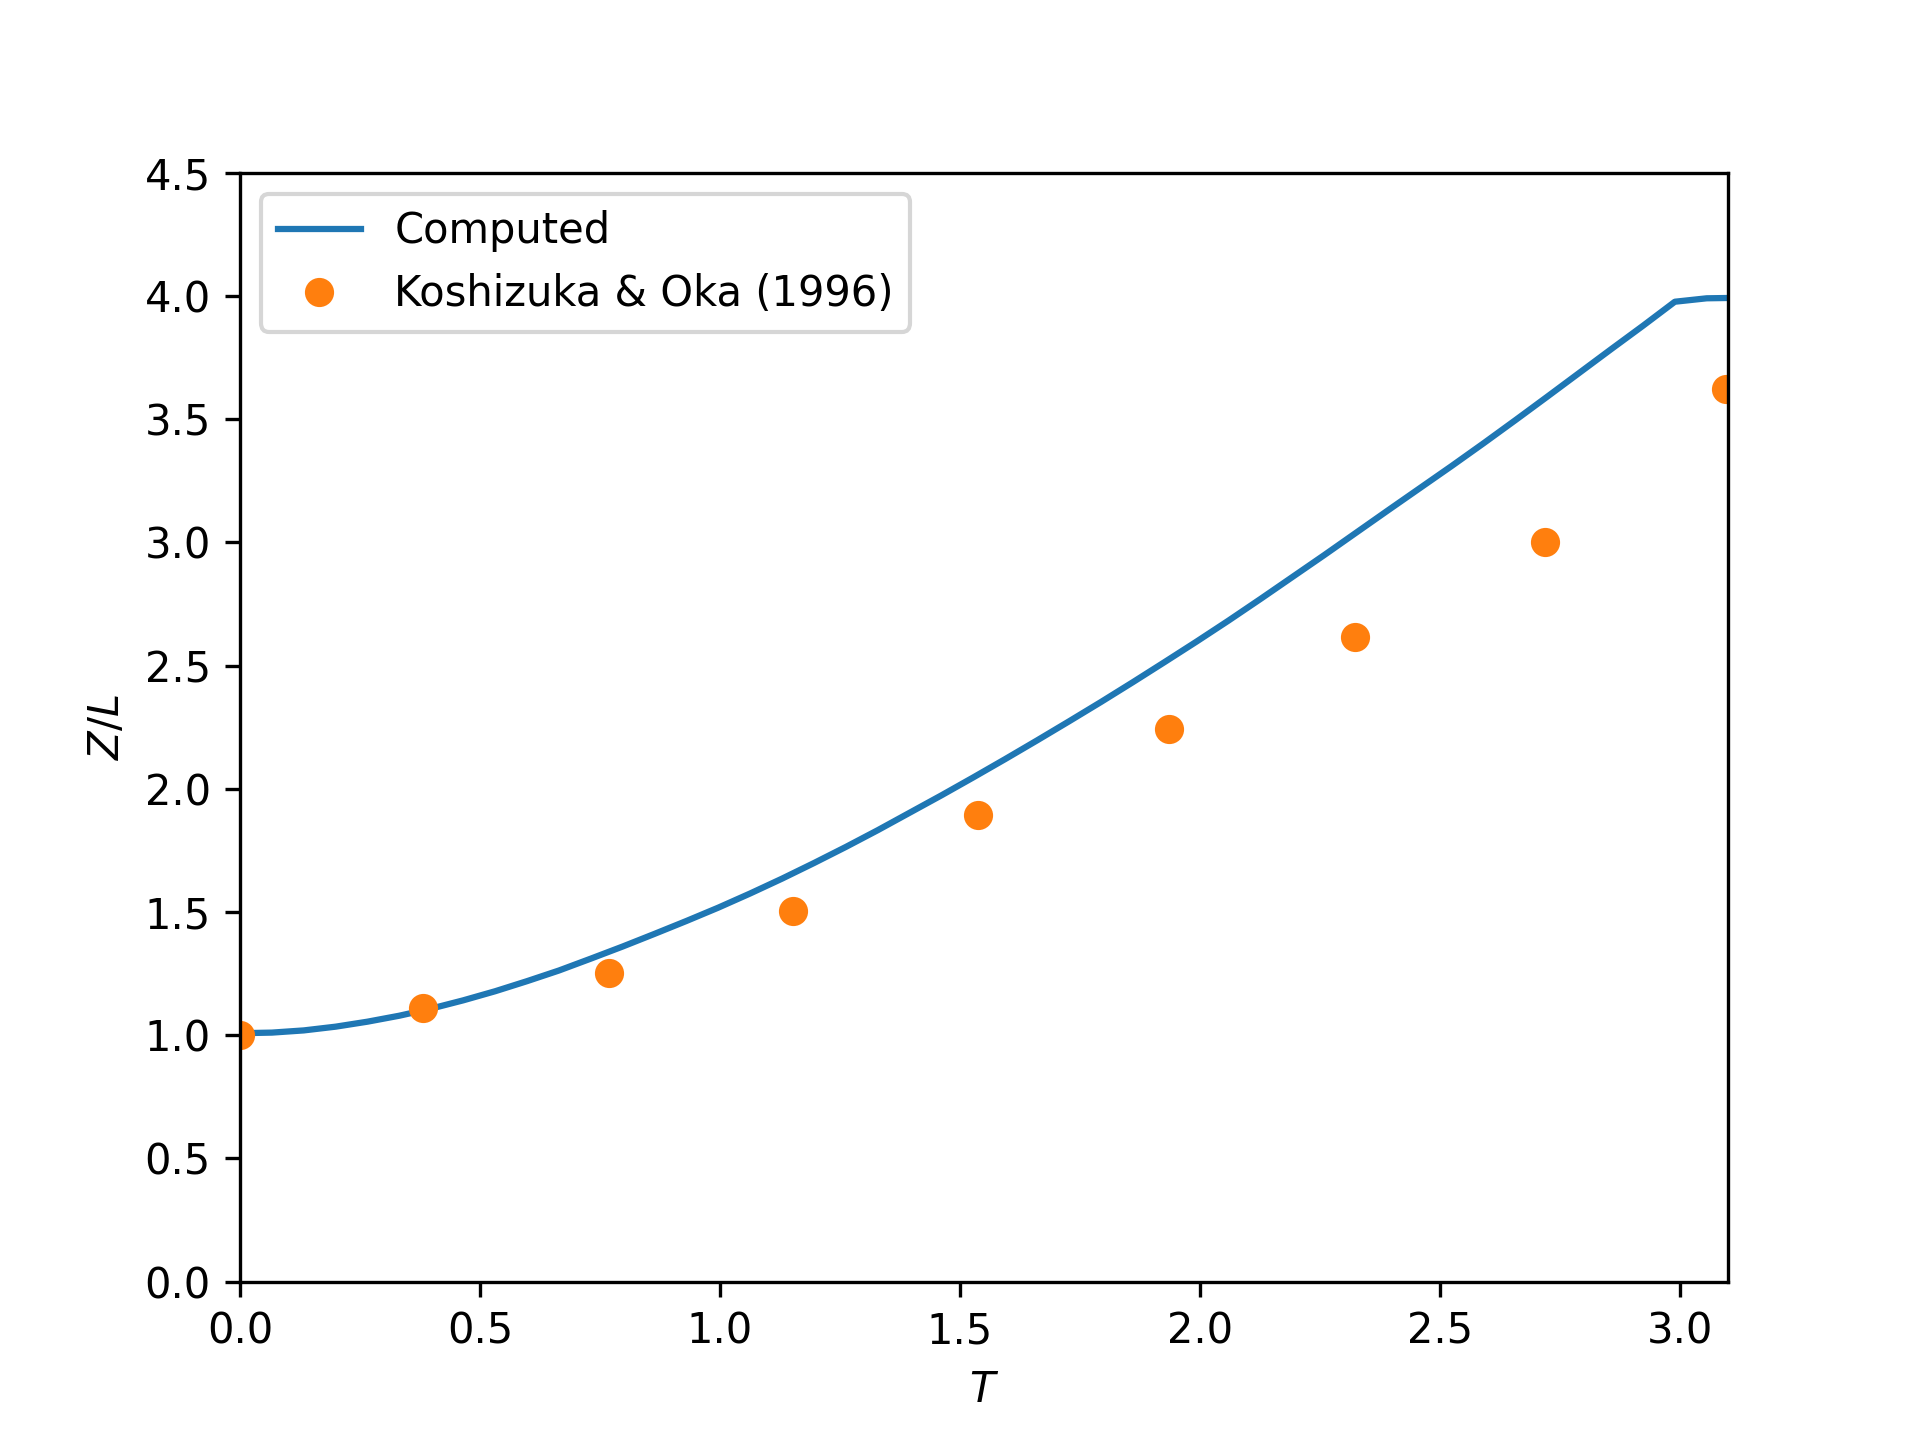
\includegraphics[width=0.8\textwidth]{figures/ctvf/figures/dam_break_2d/etvf_sun2019/x_vs_t}
  \caption{Position of the toe of the water versus time of CTVF as compared
    with the simulation of ~\citep{koshizuka1996moving}. Z is the
    distance of toe of the dam from the left wall and L is the initial width
    of the dam}
\label{fig:dam-break}
\end{figure}

\Cref{fig:dam-break} compares the position of the toe of the fluid block with
time against \citep{koshizuka1996moving}, where the authors use the moving
particle semi-implicit scheme to simulate the same.

The evolution of the fluid at three different time instants t$=0.6, 1.1, 2.0$
seconds, is shown in \cref{fig:dam-break-plots-vmag}. As can be seen from
\cref{fig:dam-break-plots-vmag}, at time $2.0$ seconds we have captured the void
created due to the splashing of the fluid. The colors in
\cref{fig:dam-break-plots-vmag} shows the velocity magnitude.

%
\begin{figure}
  \centering
  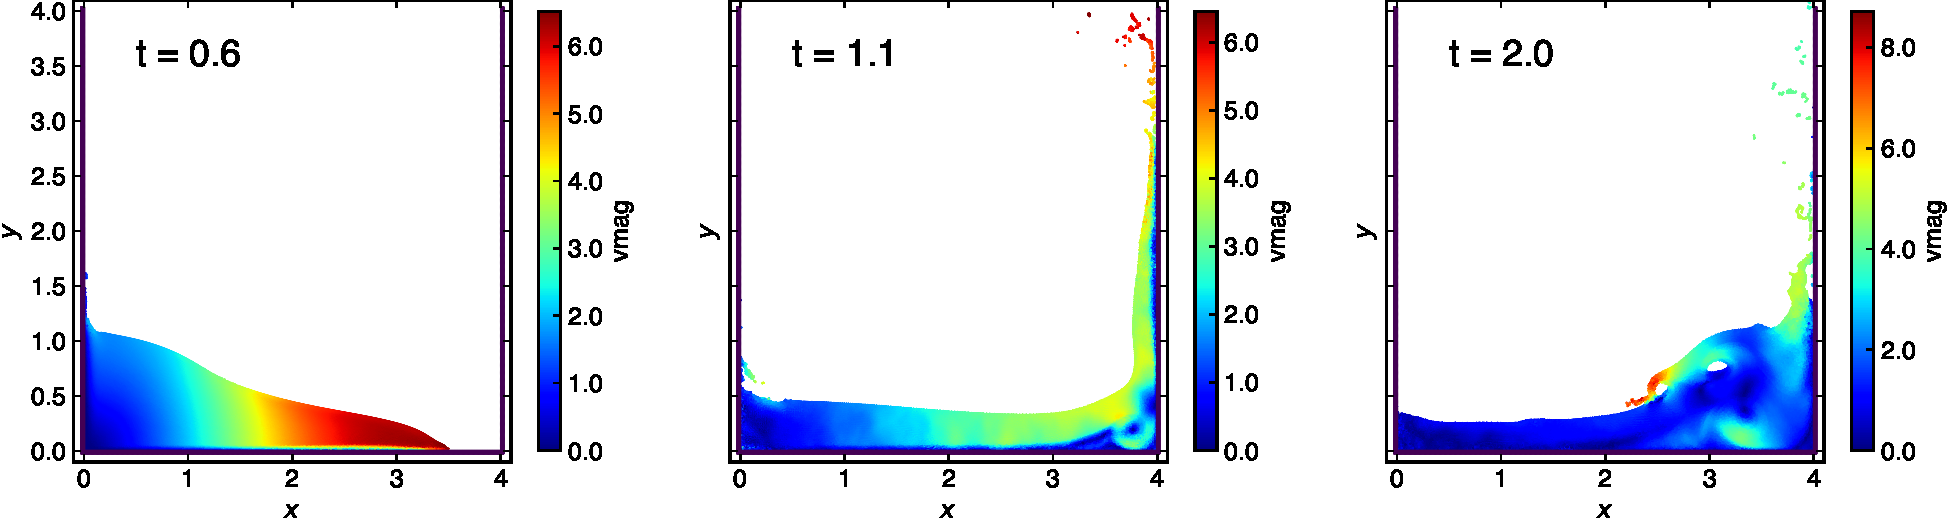
\includegraphics[width=\textwidth]{figures/ctvf/figures/dam_break_2d/db2d_vmag}
  \caption{Particle plots of fluid in dam break at time $t=0.6, 1.1, 2.0$
    second, showing velocity magnitude as contour.}
\label{fig:dam-break-plots-vmag}
\end{figure}


\FloatBarrier%
\subsection{Oscillating Plate}
\label{sec:oscillating-plate}
In this section, we test the improvement due to the correction terms while
simulating elastic solids. We show the elimination of tensile instability
while extending the transport velocity formulation~\citep{Adami2013} scheme to
more particle shifting techniques. We consider a thin oscillating
plate that is clamped on one side. \cite{landau1960} provide an analytical
solution for this problem. This is also simulated numerically in
\citep{gray-ed-2001} and \citep{zhang_hu_adams17}.


An oscillating plate with a length of $0.2$ m and a height of $0.02$ m is
initially given with a velocity profile of,
%
\begin{equation*}
  v_y(x) = V_f \, c_0 \frac{F(x)}{F(L)},
\end{equation*}
where $V_f$ varies for different cases. $L$ is the length of the plate. $F(x)$
is given by,
\begin{multline}
  F(x) = (\cos(kL) + \cosh(kL)) \, (\cosh(kx) - \cos(kx)) + \\
  (\sin(kL) - \sinh(kL)) \, (\sinh(kx) - \sin(kx)).
\end{multline}
%
In the present example $kL$ is 1.875. The material properties of the plate are
as follows, Young's modulus $E=2.0\times 10^6$ Pa, a Poisson's ratio of
$\nu=0.3975$. $c_0$ is speed of sound, and a density of $\rho=1000$
kg\,m\textsuperscript{-3}, as done in~\citep{gray-ed-2001}.  In all the cases
simulated here, we use an $\alpha$ of $1$ for artificial viscosity.

The GTVF~\citep{zhang_hu_adams17} eliminates the tensile instability while
using the special PST proposed in the original paper. We show that the
GTVF~\citep{zhang_hu_adams17} scheme is unable to eliminate numerical fracture
when a different PST algorithm is employed. Instead of using
the standard GTVF homogenization acceleration we use Sun's particle shifting
technique (SPST). This results in a numerical fracture, as seen in
\cref{fig:oscillating-plate:gtvf-sun2019-b}. We reproduced the same case with
original GTVF scheme, where no numerical fracture has found as seen in
\cref{fig:oscillating-plate:gtvf-sun2019-a}. This numerical fracture is
eliminated by the current scheme. This is due to the incorporation of the
additional terms in the current scheme as well as the use of momentum velocity
in the computation of the velocity gradient. Note that a particle spacing of
$\Delta x=0.002$ m and $V_f=0.05$ m\,s\textsuperscript{-1} has been used.

%
%
\begin{figure}
  \centering
  \begin{subfigure}{0.48\textwidth}
    \centering
    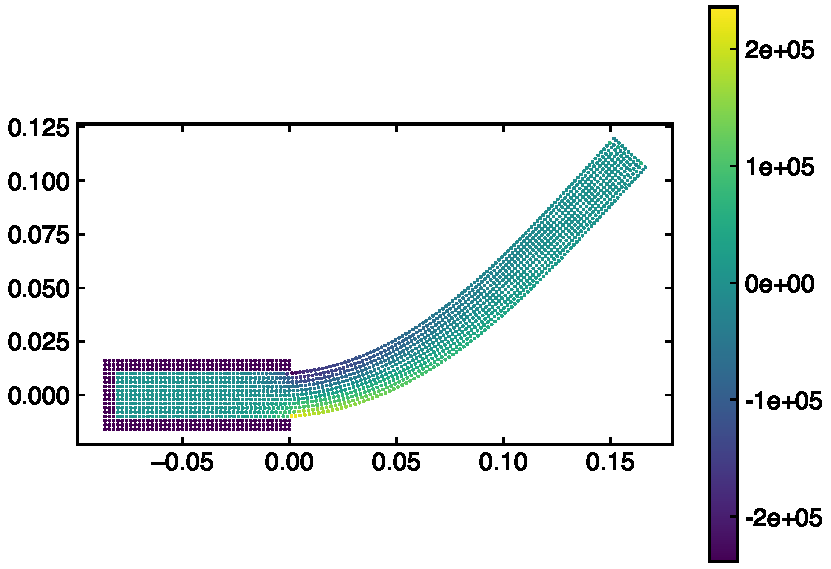
\includegraphics[width=0.8\textwidth]{figures/ctvf/figures/oscillating_plate_gtvf/gtvf_original}
    \subcaption{}%
    \label{fig:oscillating-plate:gtvf-sun2019-a}
  \end{subfigure}
  %
  \begin{subfigure}{0.48\textwidth}
    \centering
    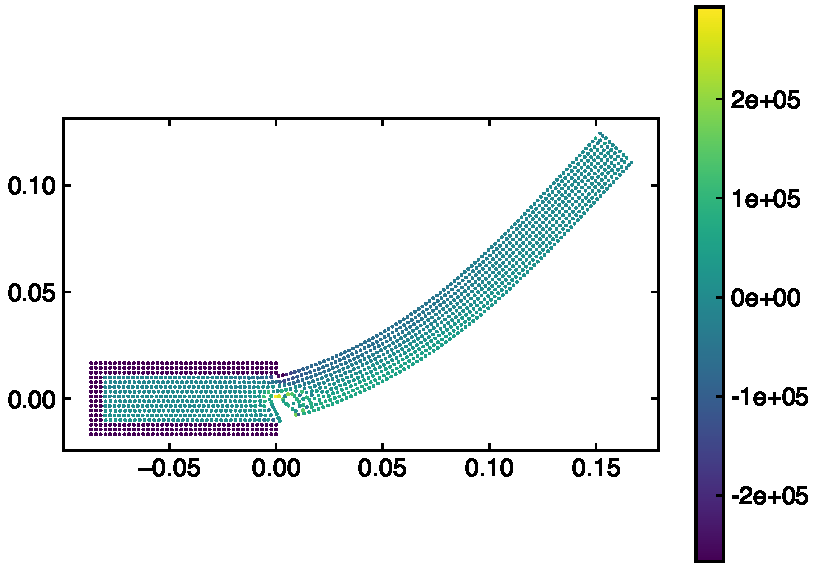
\includegraphics[width=0.8\textwidth]{figures/ctvf/figures/oscillating_plate/gtvf_sun2019}
    \subcaption{}%
    \label{fig:oscillating-plate:gtvf-sun2019-b}
  \end{subfigure}
\caption{Oscillating plate with a length of $0.2$m and height of $0.02$m when
  simulated with GTVF Scheme. Figure in left is original GTVF scheme and right
  is while using SPST with GTVF scheme.}
\end{figure}
%


This is further demonstrated by a case where an oscillating plate of length of
$0.2$ m and a height of $0.02$ m is simulated for a time of $0.22$ seconds.
Similarly, another case where plate of height $0.01$ m and a width of $0.2$ m is
run for a time of $0.51$ s.
\Cref{fig:oscillating-plate:etvf-sun2019-l-0-2-h-0-22} and
\cref{fig:oscillating-plate:etvf-sun2019-l-0-2-h-0-01} shows particles of the
plate at time $t=0.22$ s and $0.51$ s of these two cases respectively.
\Cref{fig:oscillating-plate:etvf-ipst-l-0-4-h-0-02} shows the snapshot of an
oscillating plate of length of $0.4$ m and a height of $0.02$ m, with $V_f$
equal to $0.08$ m\,s\textsuperscript{-1}.
\Cref{fig:oscillating-plate:etvf-ipst-l-0-4-h-0-02} depicts the large
deformation of the oscillating plate simulated with the current solver. We can
see from the
\cref{fig:oscillating-plate:etvf-sun2019-l-0-2-h-0-22,fig:oscillating-plate:etvf-sun2019-l-0-2-h-0-01,fig:oscillating-plate:etvf-ipst-l-0-4-h-0-02},
that the plate is free of numerical fracture. Thus we can say that the current
solver is able to eliminate tensile instability with particle shifting
techniques for problems involving small and large deformations.

%
%
\begin{figure}
  \centering
  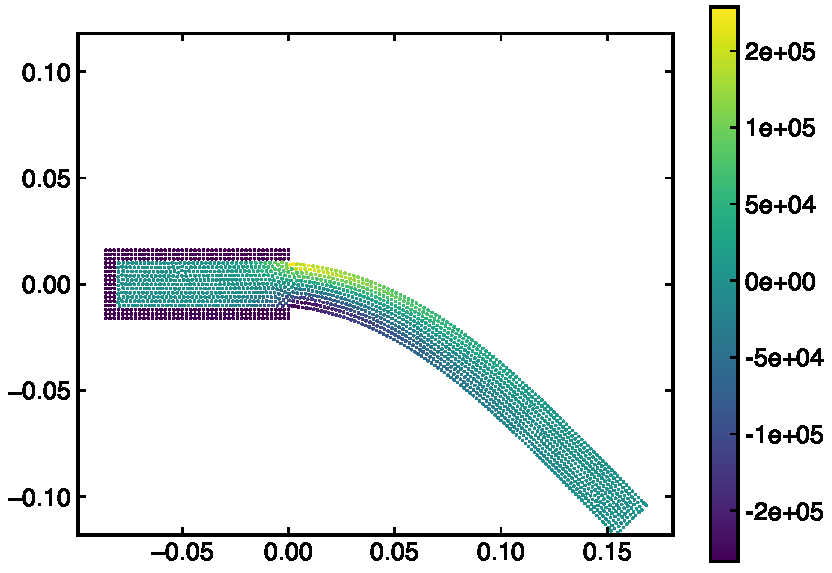
\includegraphics[width=0.8\columnwidth]{figures/ctvf/figures/oscillating_plate/etvf_sun2019_l_0_2_h_0_02}
  \caption{Oscillating plate at time $t=0.22$s with a length of $0.2$m and
    height of $0.02$m simulated with SPST with CTVF scheme.}
\label{fig:oscillating-plate:etvf-sun2019-l-0-2-h-0-22}
\end{figure}
%
%
\begin{figure}[!htp]
  \centering
  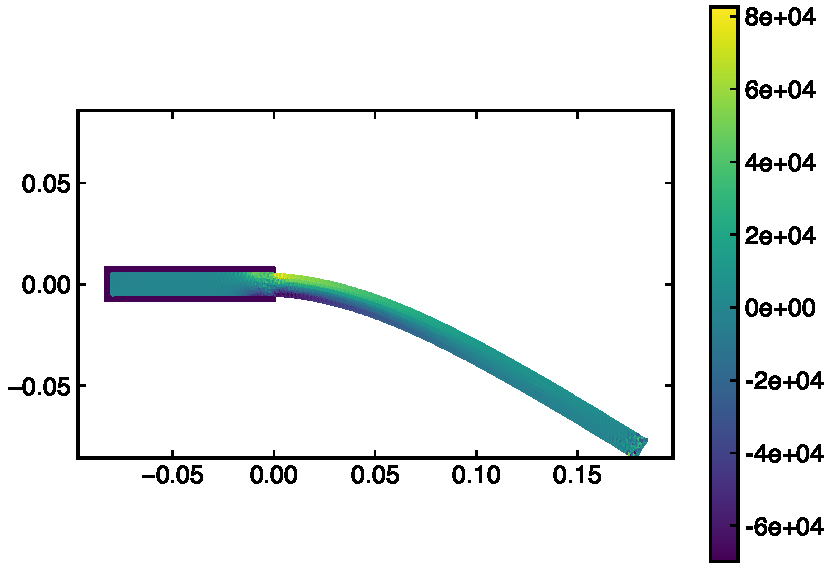
\includegraphics[width=0.8\columnwidth]{figures/ctvf/figures/oscillating_plate/etvf_sun2019_l_0_2_h_0_01}
  \caption{Oscillating plate at time $t=0.51$s with a length of $0.2$m and
    height of $0.01$m simulated with SPST with CTVF scheme.}
\label{fig:oscillating-plate:etvf-sun2019-l-0-2-h-0-01}
\end{figure}
%
%
\begin{figure}[!htpb]
  \centering
  \includegraphics[width=0.8\textwidth]{figures/oscillating_plate_large_deformation/ctvf_ipst}
  \caption{Oscillating plate at time $t=0.359$ seconds with a length of $0.4$m and
    height of $0.02$m simulated with IPST with CTVF scheme.}
\label{fig:oscillating-plate:etvf-ipst-l-0-4-h-0-02}
\end{figure}

The accuracy of the current scheme is evaluated by comparing with the
analytical results and with a convergence study. In
\cref{table:compare-analytical-with-simulated-h-l-0-1} we compare the time
period for the oscillation by the analytical and the numerical results with
varying $V_f$, where we consider an oscillating plate whose $H/L$ ratio is
$0.1$. The difference between the analytical result and the numerical result
is due to the fact that the analytical results are based on thin plate theory
where as the plate considered here has a finite thickness. Further, we can see
that the current numerical results are in agreement with the previously
reported numerical results~\citep{gray-ed-2001, zhang_hu_adams17}. In
\cref{fig:oscillating:ipst_convergence_plot}, we have performed a convergence
study of an oscillating plate, with a $\nu=0.3975$, and $V_f=0.05$
m\,s\textsuperscript{-1}, and IPST is used for particle homogenization. The trend of
the current scheme matches well with the other updated Lagrangian SPH
schemes~\citep{gray-ed-2001, zhang_hu_adams17}. Hence the current scheme is
able to work with different PST methods and removes the tensile instability.

\begin{table}[!htpb]
\centering
\begin{tabular}{c c c c c}
  \hline
  $V_f$ & 0.001 & 0.01 & 0.03 & 0.05 \\
  \hline
  $\text{T}_{\mathrm{CTVF}}$ & 0.284 & 0.283 & 0.283 & 0.284 \\
  $\text{T}_{\mathrm{GTVF}}$ & 0.284 & 0.283 & 0.284 & 0.285 \\
  $\text{T}_{\mathrm{analytical}}$ & 0.254 & 0.252 & 0.254 & 0.254
\end{tabular}
\caption{Comparison between the CTVF and the analytical solution for the time
  period of the oscillating plate with a length of $0.2$m and height of
  $0.02$m with various $V_f$}
\label{table:compare-analytical-with-simulated-h-l-0-1}
\end{table}
\begin{figure}
  \centering
  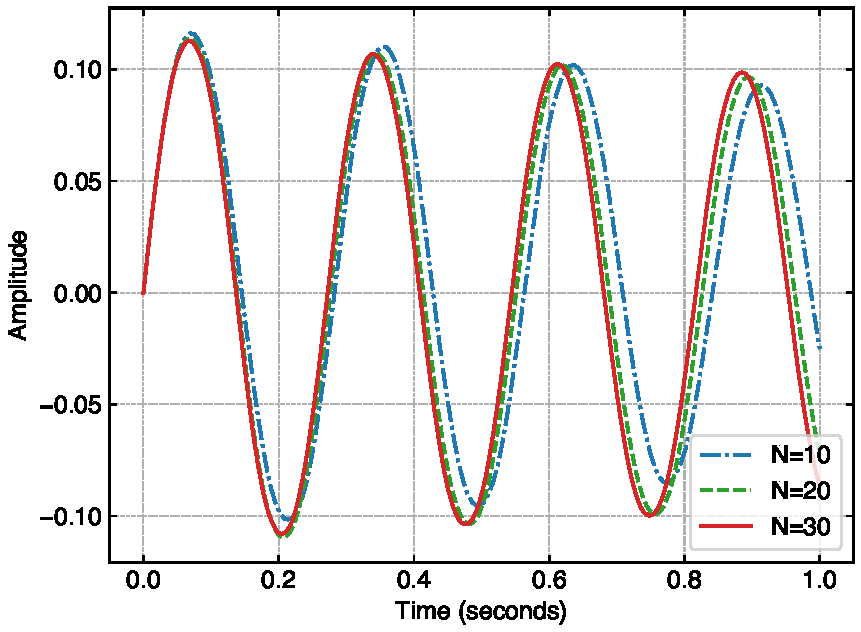
\includegraphics[width=0.7\columnwidth]{figures/ctvf/figures/oscillating_plate/ipst_convergence_plot}
  \caption{The vertical position of the particle at the end of the plate as a
    function of time. Here we consider a three particle variations, 10, 20 and
    30 particles across the plate width.}
\label{fig:oscillating:ipst_convergence_plot}
\end{figure}
%

%
%
%
%
\FloatBarrier%
\subsection{Uniaxial Compression}
\label{sec:uniaxial-compression}

This benchmark is used to test the proposed scheme. A uniaxial bar is
compressed by a moving piston on top of it. This problem has been simulated by
\cite{das2015evaluation}. We compare the von Mises stress at the center point
of the bar with the result of the FEM analysis and SPH provided in
\citep{das2015evaluation}.

The numerical model consists of three parts. It has an axially loaded
rectangular specimen of width $82$ mm and height of $140$ mm. The specimen has
the properties of a sand stone (Crossley Sandstone) with a Young's modulus of
$7.5$ GPa and Poisson ratio of $0.398$ and with a density of $2300$
kg\,m\textsuperscript{-3}. The speed of sound resulting from such properties is
$2303$ m\,s\textsuperscript{-1}. We run three particle resolutions,
$\Delta x = 0.5$ mm, $1$ mm and $2$ mm. The particles are placed on a regular
square grid pattern. The velocity of the top plate is
$1.5$ mm\,s\textsuperscript{-1}, which is used to apply the load on the specimen in
such a fashion, such that the loaded end is deformed at the required constant
rate. This is described in \cref{fig:uniaxial_test_configuration}. An $\alpha$
of $1$ is used in the current simulation for the artificial viscosity.

\begin{figure}[!htp]
  \centering
  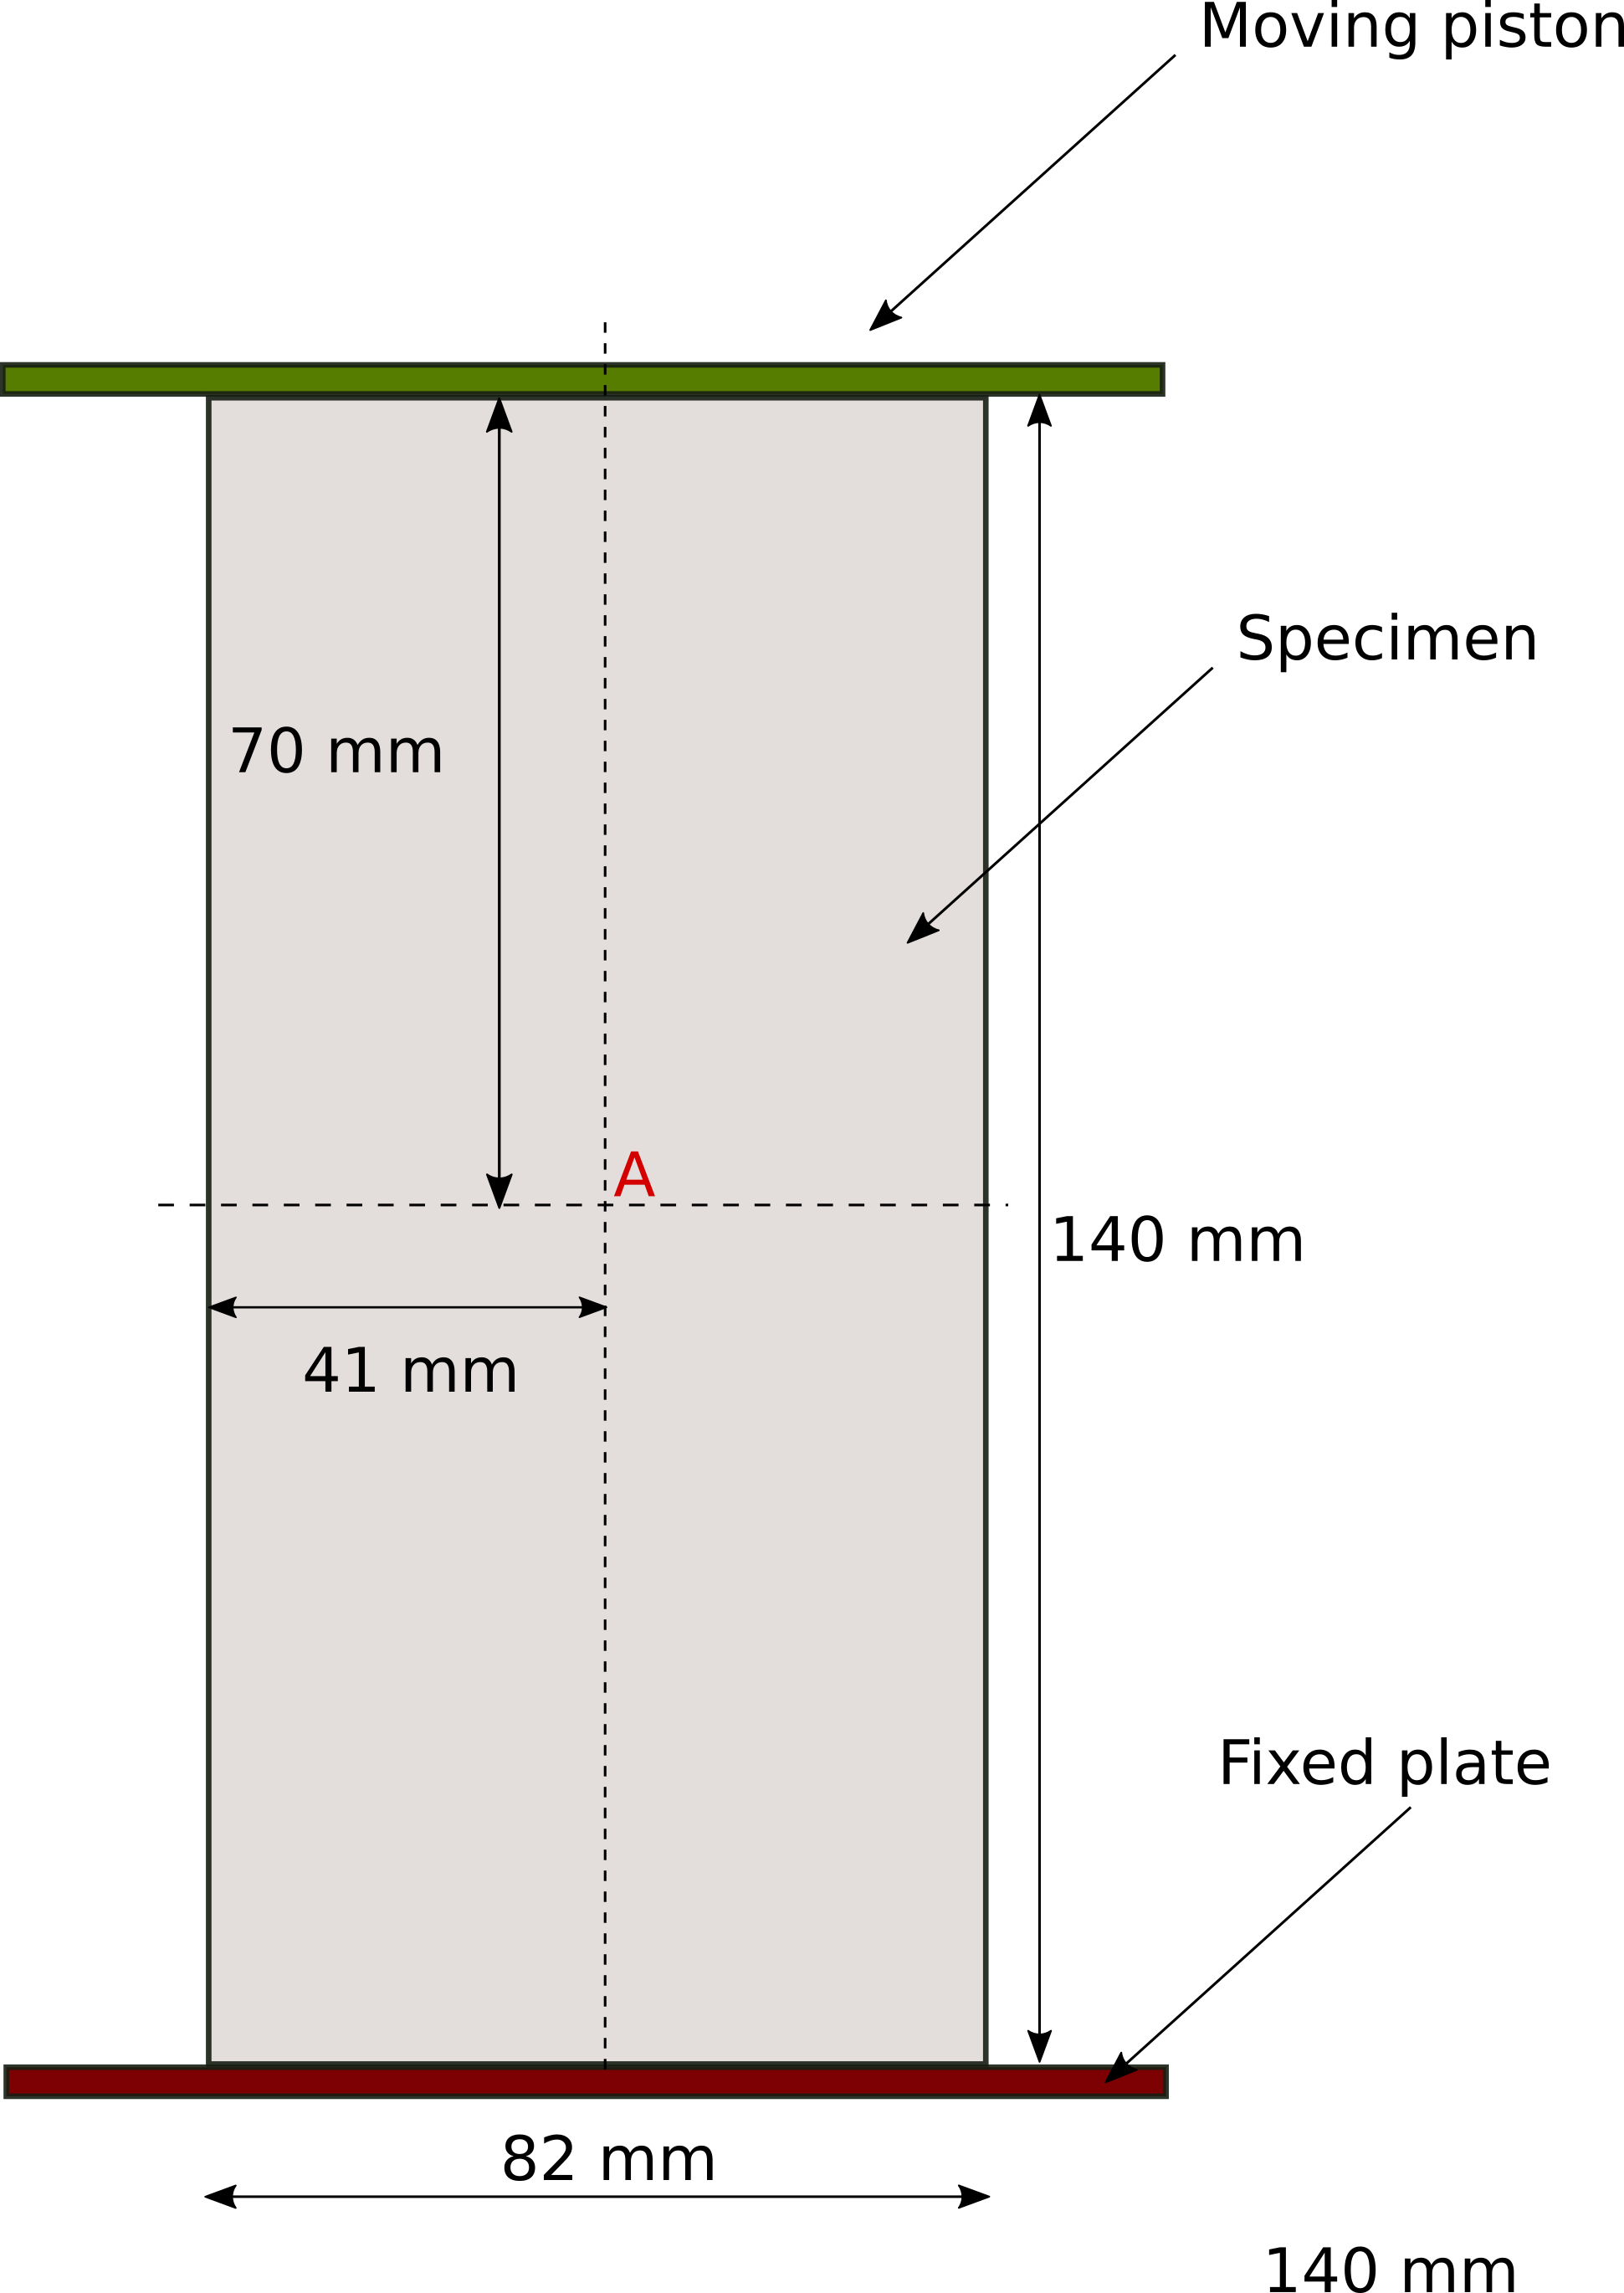
\includegraphics[width=0.4\textwidth]{images/ctvf/images/uniaxial_compression/uniaxial_compression}
  \caption{Test configuration of sand stone under uniaxial compression.}
\label{fig:uniaxial_test_configuration}
\end{figure}


We use the von Mises stress as the criterion for analysing the stress field.
It combines the normal and shear components of the deviatoric stress tensor,
and is a commonly used criterion to assess failure strength of materials. The
von Mises stress $\sigma_{vm}$ can be expressed in 2D in terms of principle
stress $\sigma_1$ and $\sigma_2$ as

\begin{equation}
  \label{eq:von_mises_with_principal_stress}
  \sigma_{vm} = \sqrt{\left(\sigma_1^2 + \sigma_2^2 - \sigma_1 \ \sigma_2\right)}
\end{equation}
%
%
Where the principal stress are found by
\begin{eqnarray}
  \label{eq:principal_stress}
  \sigma_{1} = \frac{\sigma_{xx} + \sigma_{yy}}{2} + \sqrt{\left(\bigg(
  \frac{\sigma_{xx} + \sigma_{yy}}{2}\bigg)^2 + \sigma_{xy}^2\right)}\\
  \sigma_{2} = \frac{\sigma_{xx} + \sigma_{yy}}{2} -  \sqrt{\left(\bigg(
  \frac{\sigma_{xx} + \sigma_{yy}}{2}\bigg)^2 + \sigma_{xy}^2\right)}
\end{eqnarray}
%
\begin{figure}
  \centering
  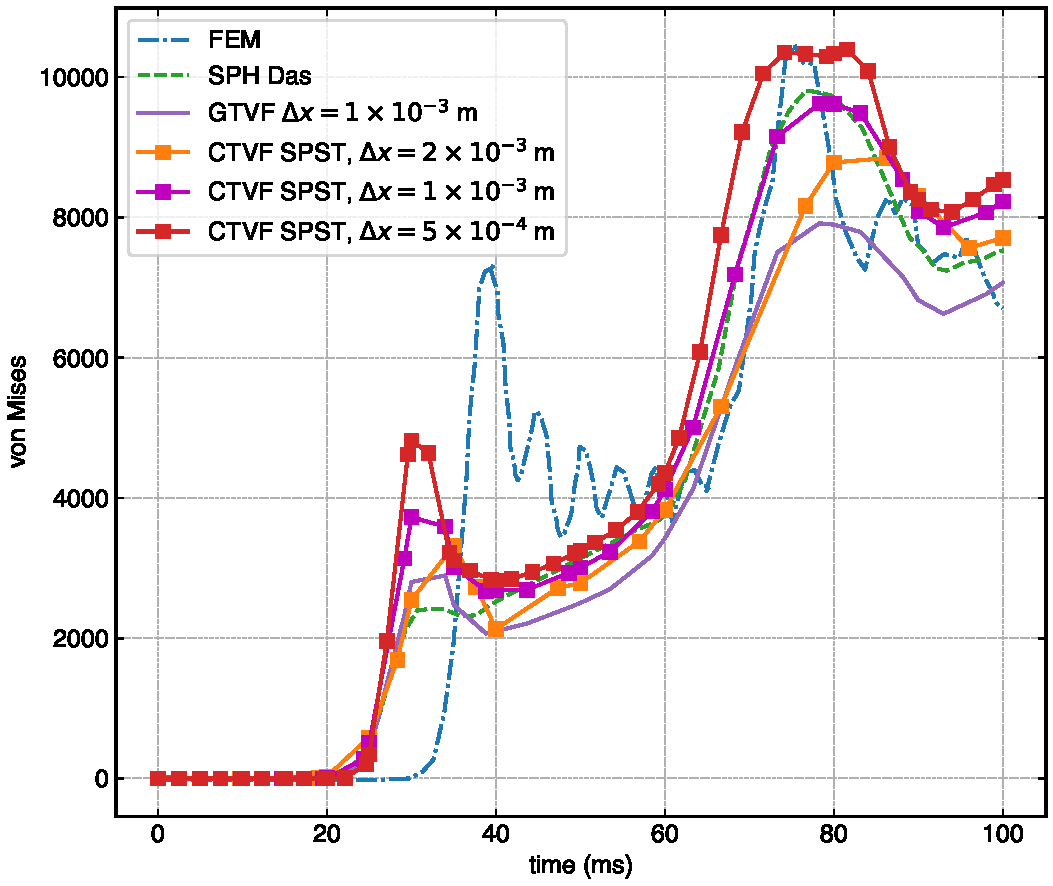
\includegraphics[width=0.8\textwidth]{figures/ctvf/figures/uniaxial_compression/von_mises_A}
  \caption{von Mises stress at point A in uniaxial compression with three
    different resolutions compared against those from
    \citep{das2015evaluation}.}
\label{fig:uniaxial}
\end{figure}

\Cref{fig:uniaxial} shows the von Mises stress versus time of the current
scheme, when simulated with three different resolutions compared against with
the finite element result and SPH result provided in \citep{das2015evaluation}.
It also shows the result with the GTVF scheme using the medium resolution. As
can be seen in \cref{fig:uniaxial} the GTVF result does not match very well
with FEM and SPH result provided by \cite{das2015evaluation}, and the current
scheme performs significantly better.

%
%
\FloatBarrier%
\subsection{Colliding Rings}
\label{colliding-rings}

Having shown the flexibility of proposed scheme to work with different PST
methods in \cref{sec:oscillating-plate}, in the current example, we compare
the robustness of the PST methods by investigating the collision of rubber
rings with different Poisson ratios. This was first studied in SPH by
\cite{swegle1995smoothed}.

The inner ring radius of the ring is $r_{min} = 0.03$ m and the outer ring
radius $r_{max} = 0.04$ m. Both the rings have the same material properties:
Young's modulus $E = 0.01$ GPa and density $\rho = 1.2 \times 10^{3}$
 kg\,m\textsuperscript{-3}. The initial speed of the rings are equal to
$v_0 = 0.12 c_0$ m\,s\textsuperscript{-1} with an initial inter particle spacing of
$\Delta x = 0.001$ m. Where $c_0$ is the speed of sound of the material. We use
an $\alpha=1$ for the artificial viscosity in the current simulation.

Two different Poisson ratios are simulated. \Cref{fig:rings:sun2019-nu-0.3975}
shows the particle positions of rings with a Poisson ratio of $0.3975$ when
simulated with SPST. The recovery of the colliding rings without any tensile
instability can be seen.

We also consider higher Poisson ratios, such as 0.47.
\Cref{fig:rings:sun2019-nu-0-47} shows the particle positions of rings when
simulated with SPST and \cref{fig:rings:ipst-nu-0-47} with IPST. Even though
both the particle shifting techniques are able to eliminate the numerical
fracture, IPST gives better results as in the distribution of particles
through out the simulation, see \cref{fig:rings:sun2019-nu-0.47-2} and
\cref{fig:rings:ipst-nu-0.47-2}. For the case where SPST is used, the final
particle distribution is not very uniform. This is not the case when IPST is
used. We can therefore say that IPST performs better than SPST.
%
\begin{figure}
  \centering
  % \begin{subfigure}{0.3\textwidth}
  %   \centering
  %   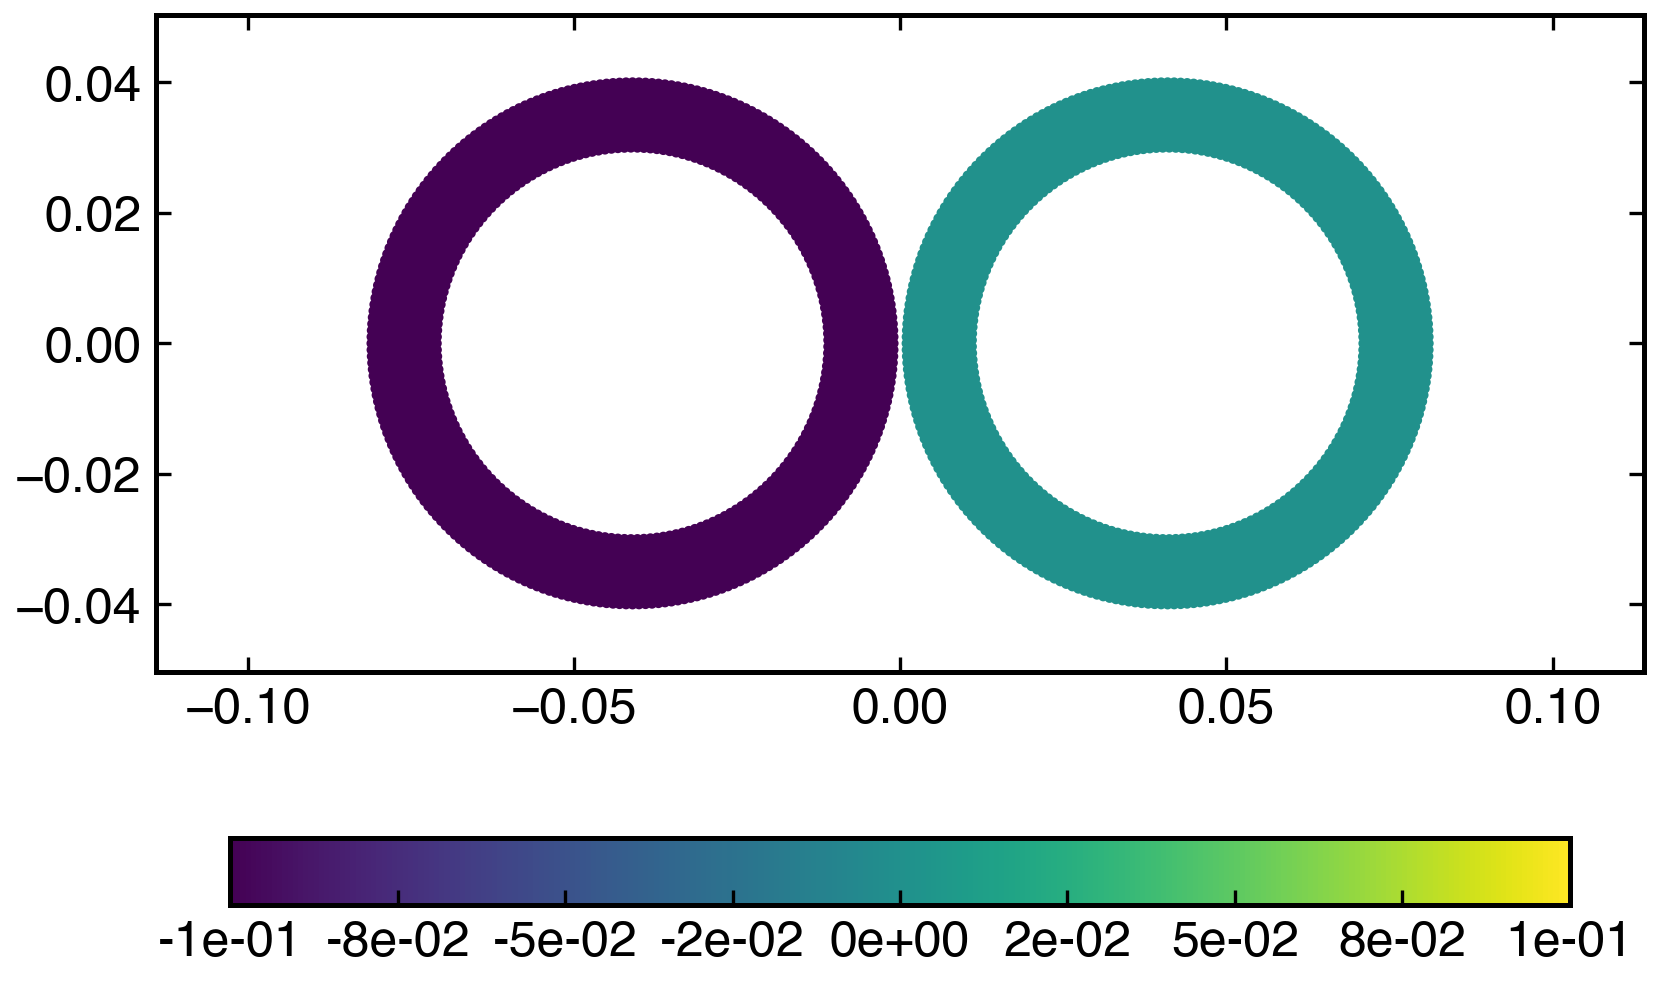
\includegraphics[width=1.0\textwidth]{figures/ctvf/figures/rings/etvf_sun2019_poisson_ratio_0.3975/time0}
  %   \subcaption{t = 0 sec}\label{fig:rings:sun2019-nu-0.3975-0}
  % \end{subfigure}
%
  \begin{subfigure}{0.48\textwidth}
    \centering
    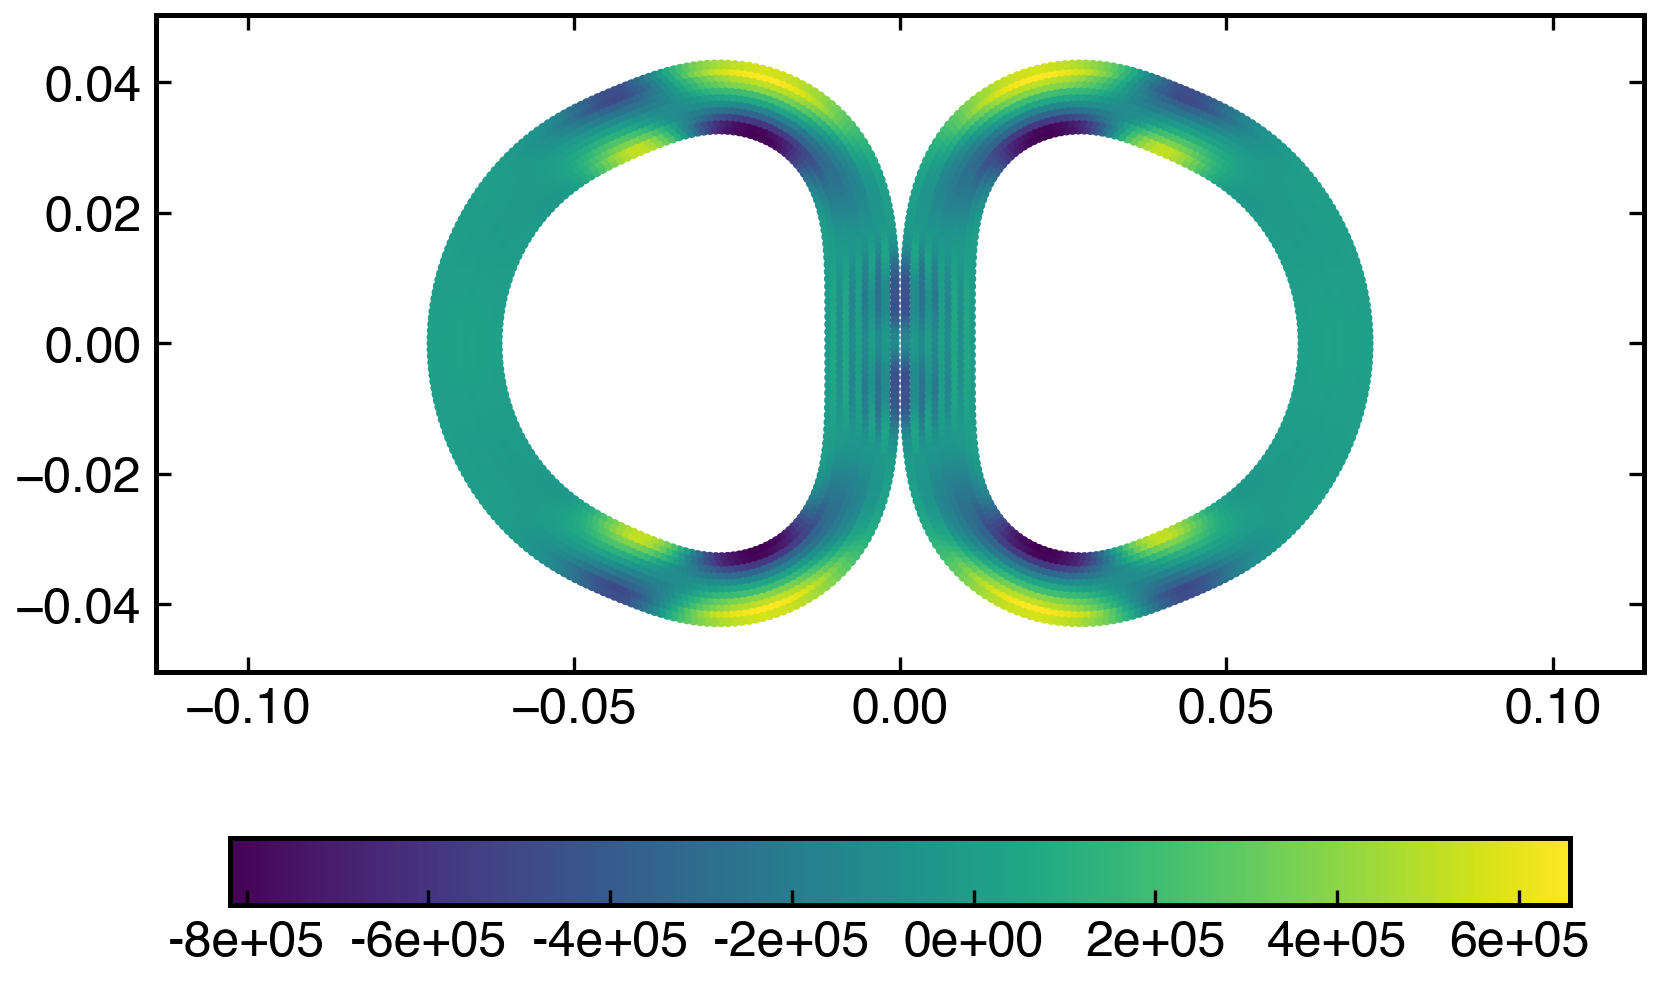
\includegraphics[width=1.0\textwidth]{figures/ctvf/figures/rings/etvf_sun2019_poisson_ratio_0.3975/time1}
    \subcaption{t = 2.5e-03 sec}\label{fig:rings:sun2019-nu-0.3975-1}
  \end{subfigure}
%
  \begin{subfigure}{0.48\textwidth}
    \centering
    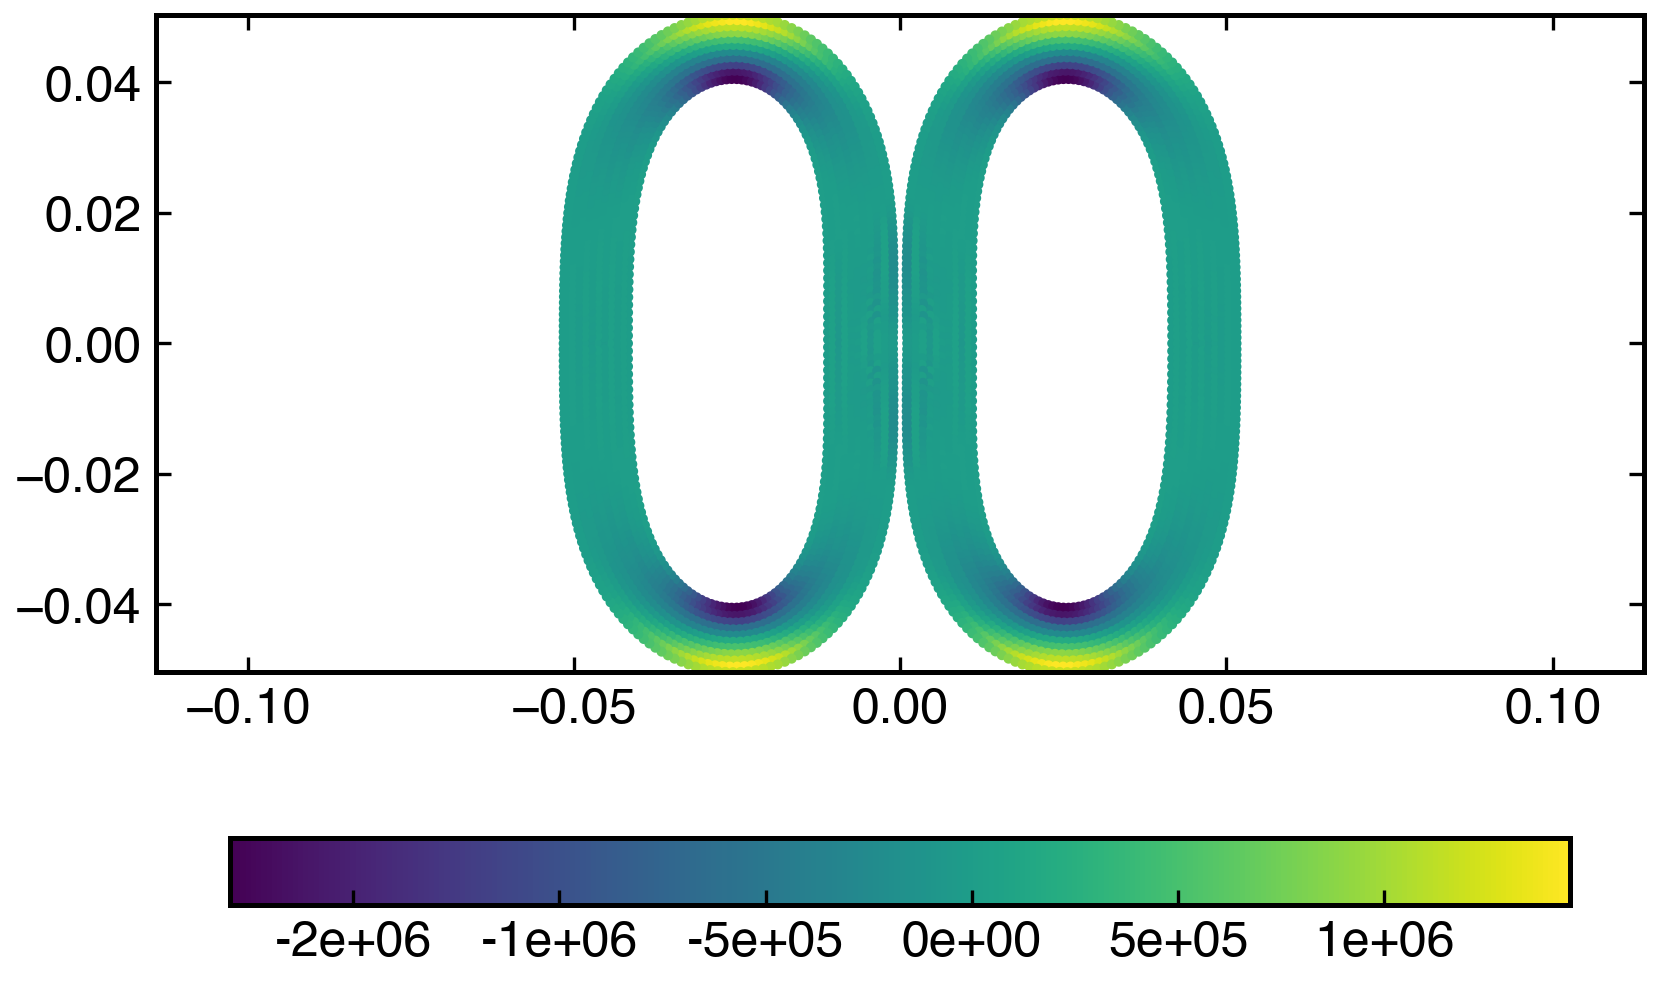
\includegraphics[width=1.0\textwidth]{figures/ctvf/figures/rings/etvf_sun2019_poisson_ratio_0.3975/time2}
    \subcaption{t = 4e-03 sec}\label{fig:rings:sun2019-nu-0.3975-2}
  \end{subfigure}

  \begin{subfigure}{0.48\textwidth}
    \centering
    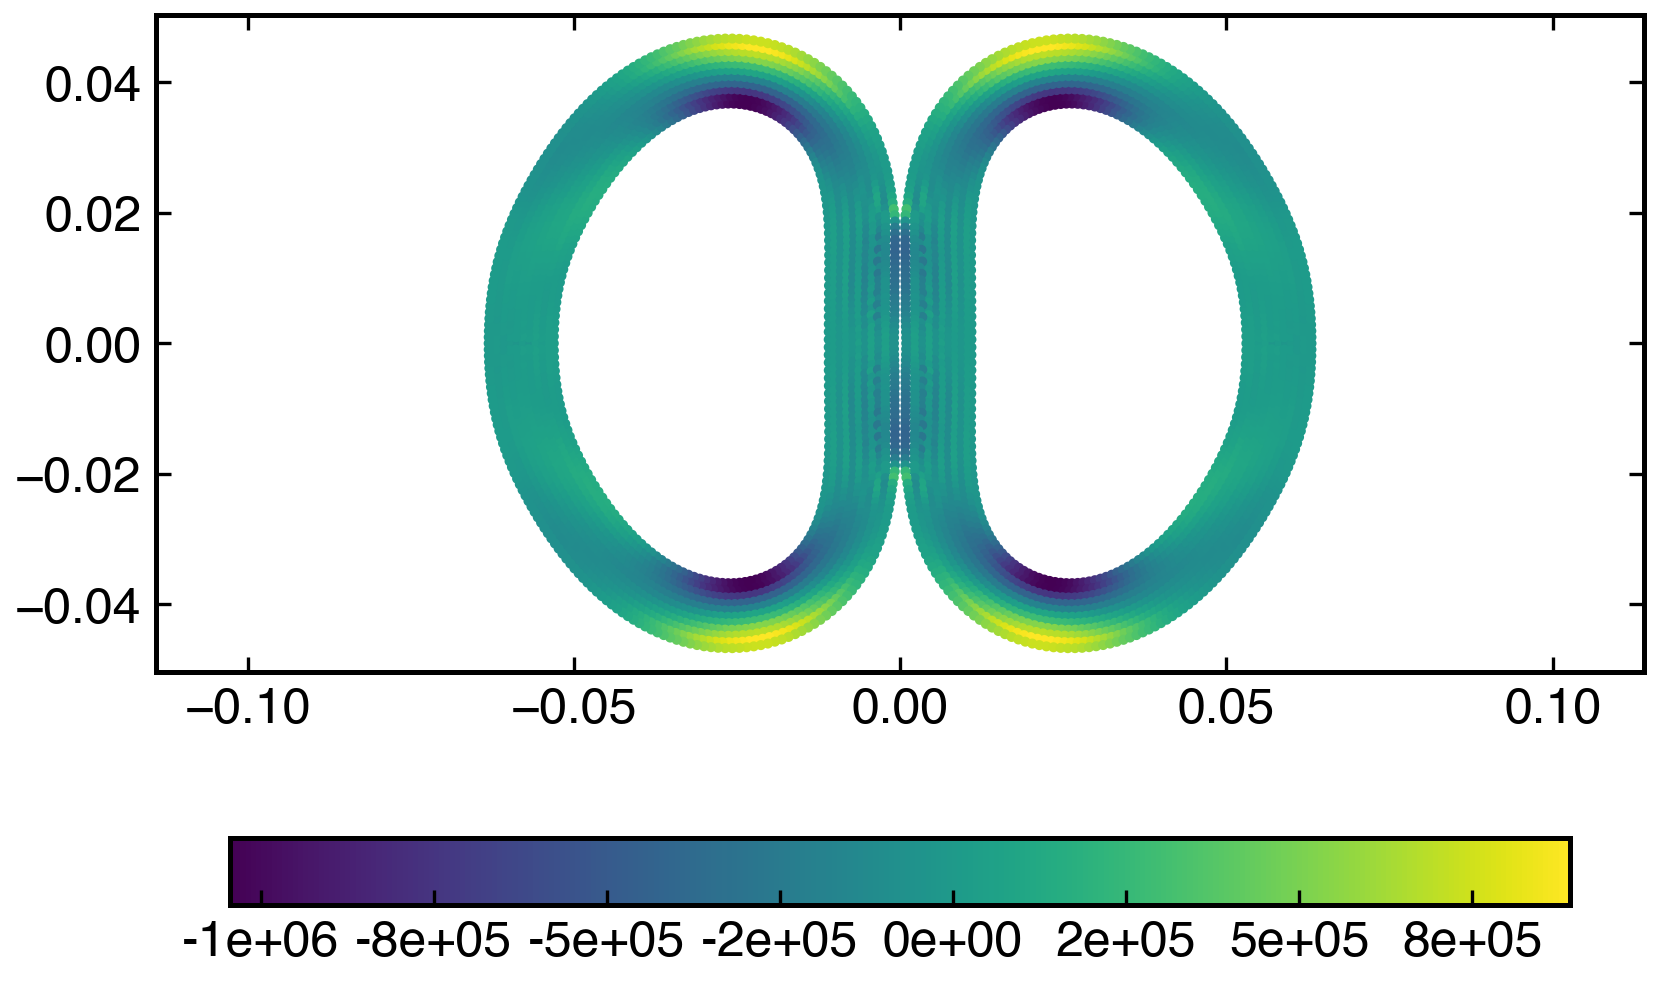
\includegraphics[width=1.0\textwidth]{figures/ctvf/figures/rings/etvf_sun2019_poisson_ratio_0.3975/time3}
    \subcaption{t = 7.3e-03 sec}\label{fig:rings:sun2019-nu-0.3975-3}
  \end{subfigure}
%
  \begin{subfigure}{0.48\textwidth}
    \centering
    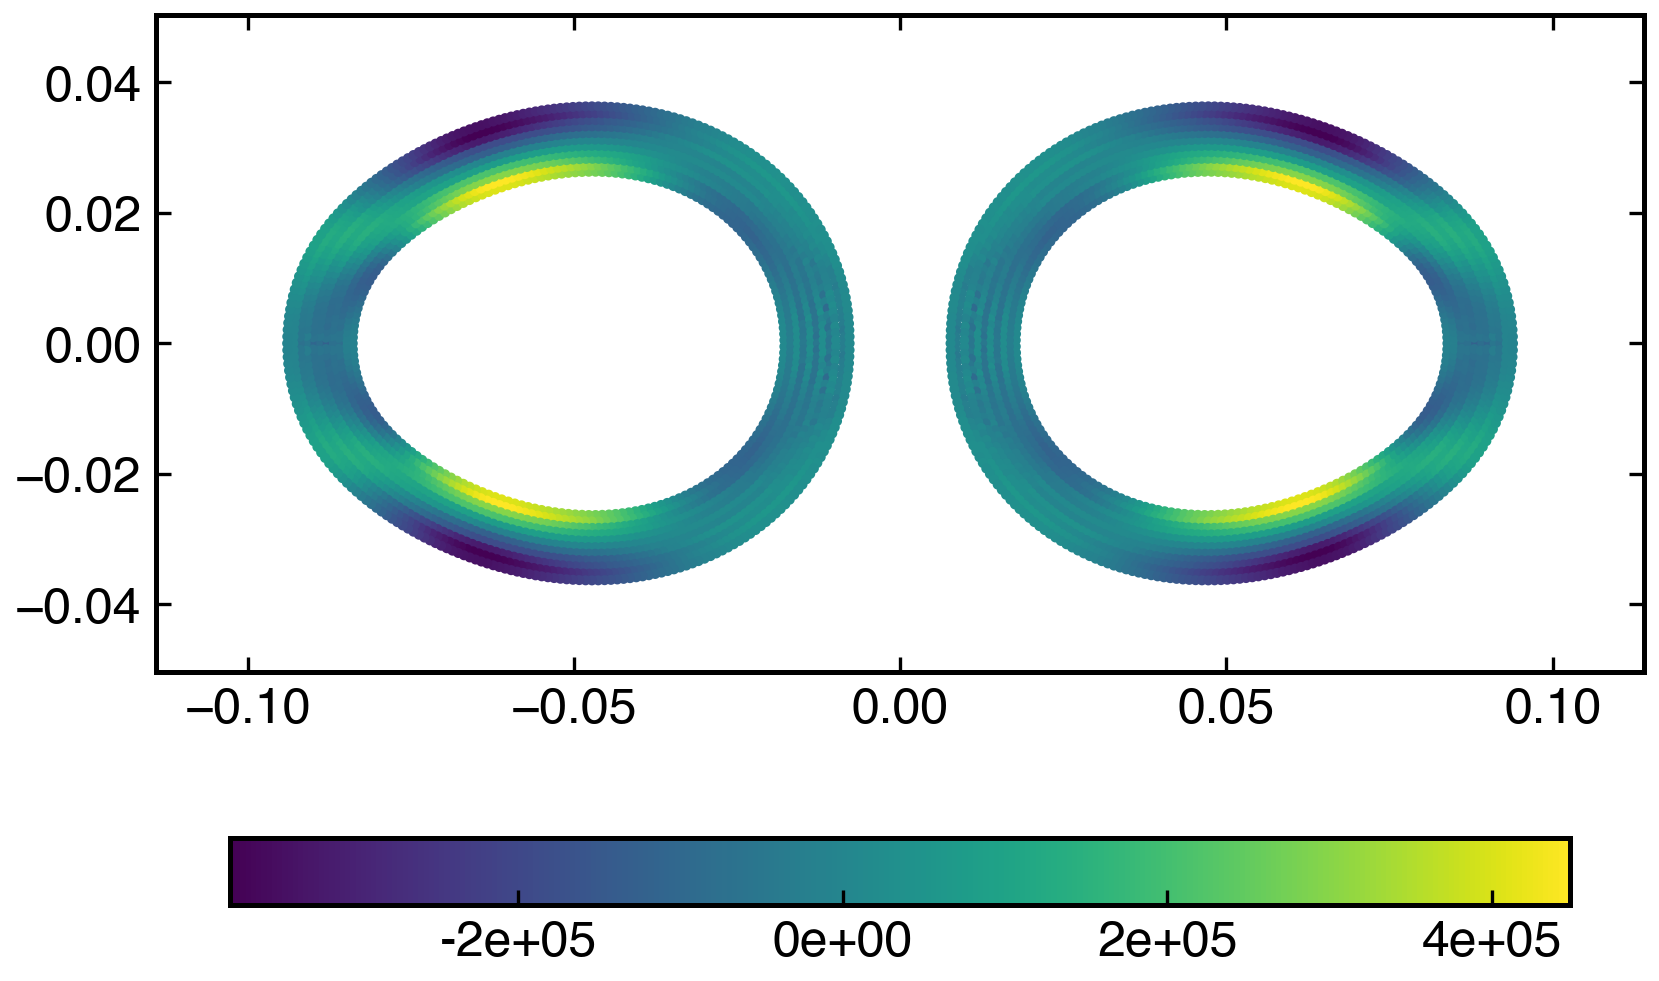
\includegraphics[width=1.0\textwidth]{figures/ctvf/figures/rings/etvf_sun2019_poisson_ratio_0.3975/time4}
    \subcaption{t = 1.45e-02 sec}\label{fig:rings:sun2019-nu-0.3975-4}
  \end{subfigure}
% %
%   \begin{subfigure}{0.3\textwidth}
%     \centering
%     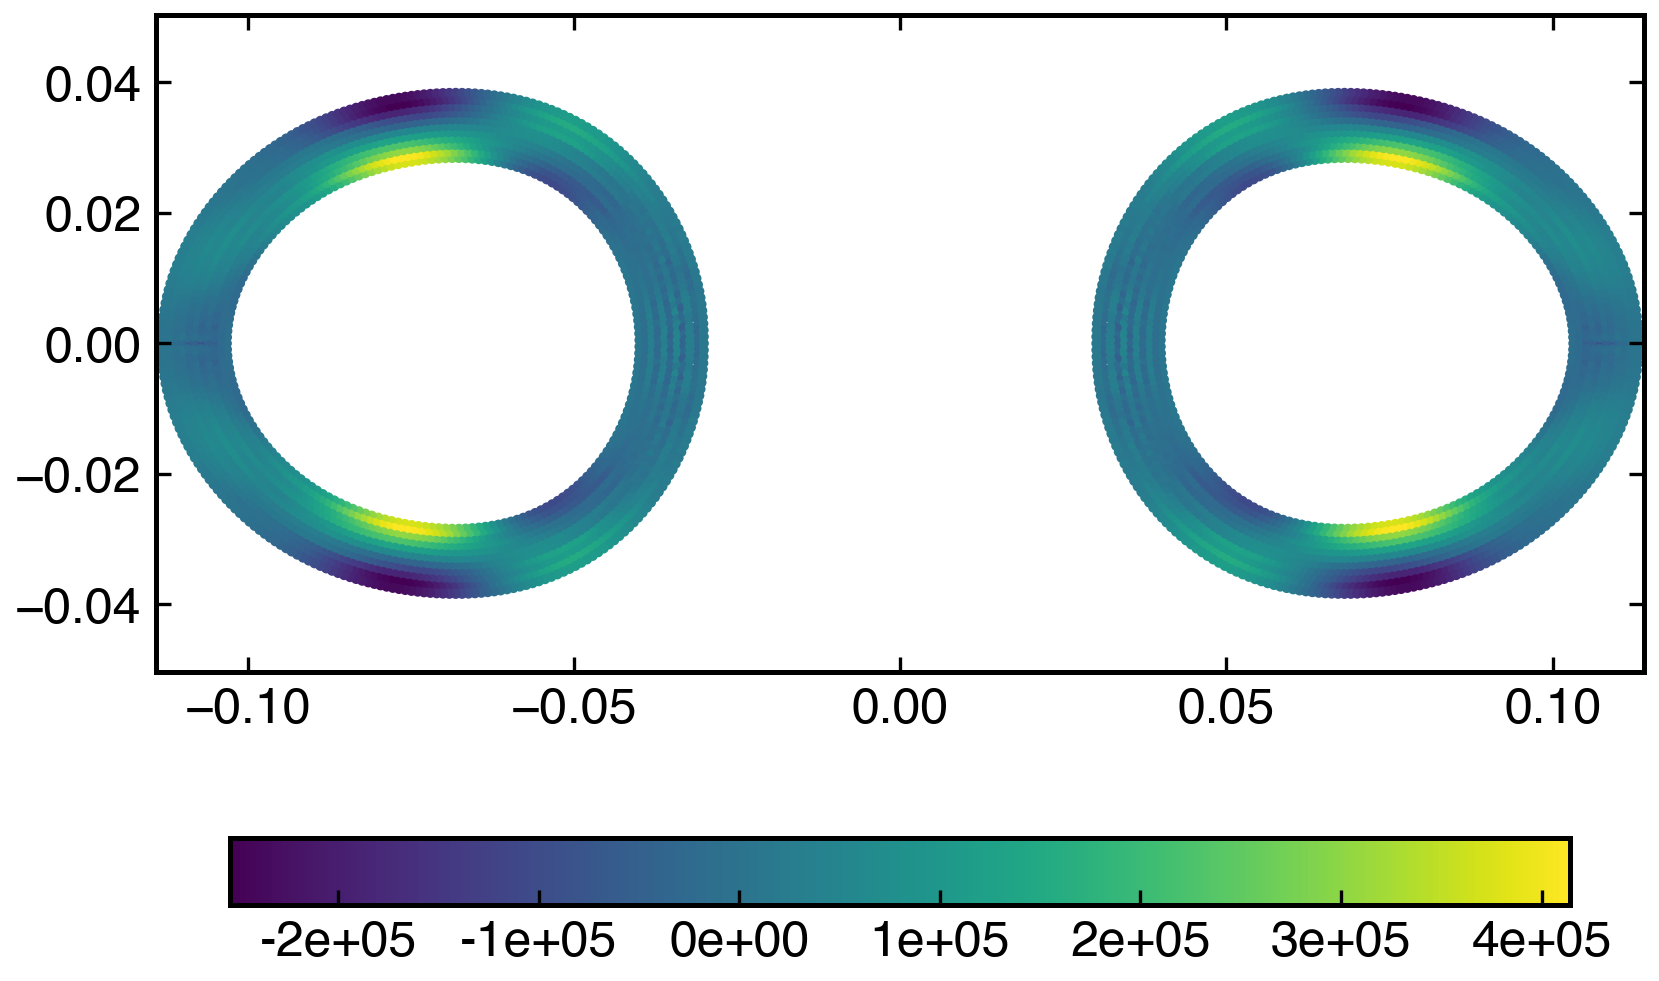
\includegraphics[width=1.0\textwidth]{figures/ctvf/figures/rings/etvf_sun2019_poisson_ratio_0.3975/time5}
%     \subcaption{t = 1.5e-02 sec}\label{fig:rings:sun2019-nu-0.3975-5}
%   \end{subfigure}
  \caption{Rings with a Poisson ratio of 0.3975 colliding head on, simulated with CTVF using SPST.}
\label{fig:rings:sun2019-nu-0.3975}
\end{figure}
%
\begin{figure}
  \centering
  % \begin{subfigure}{0.3\textwidth}
  %   \centering
  %   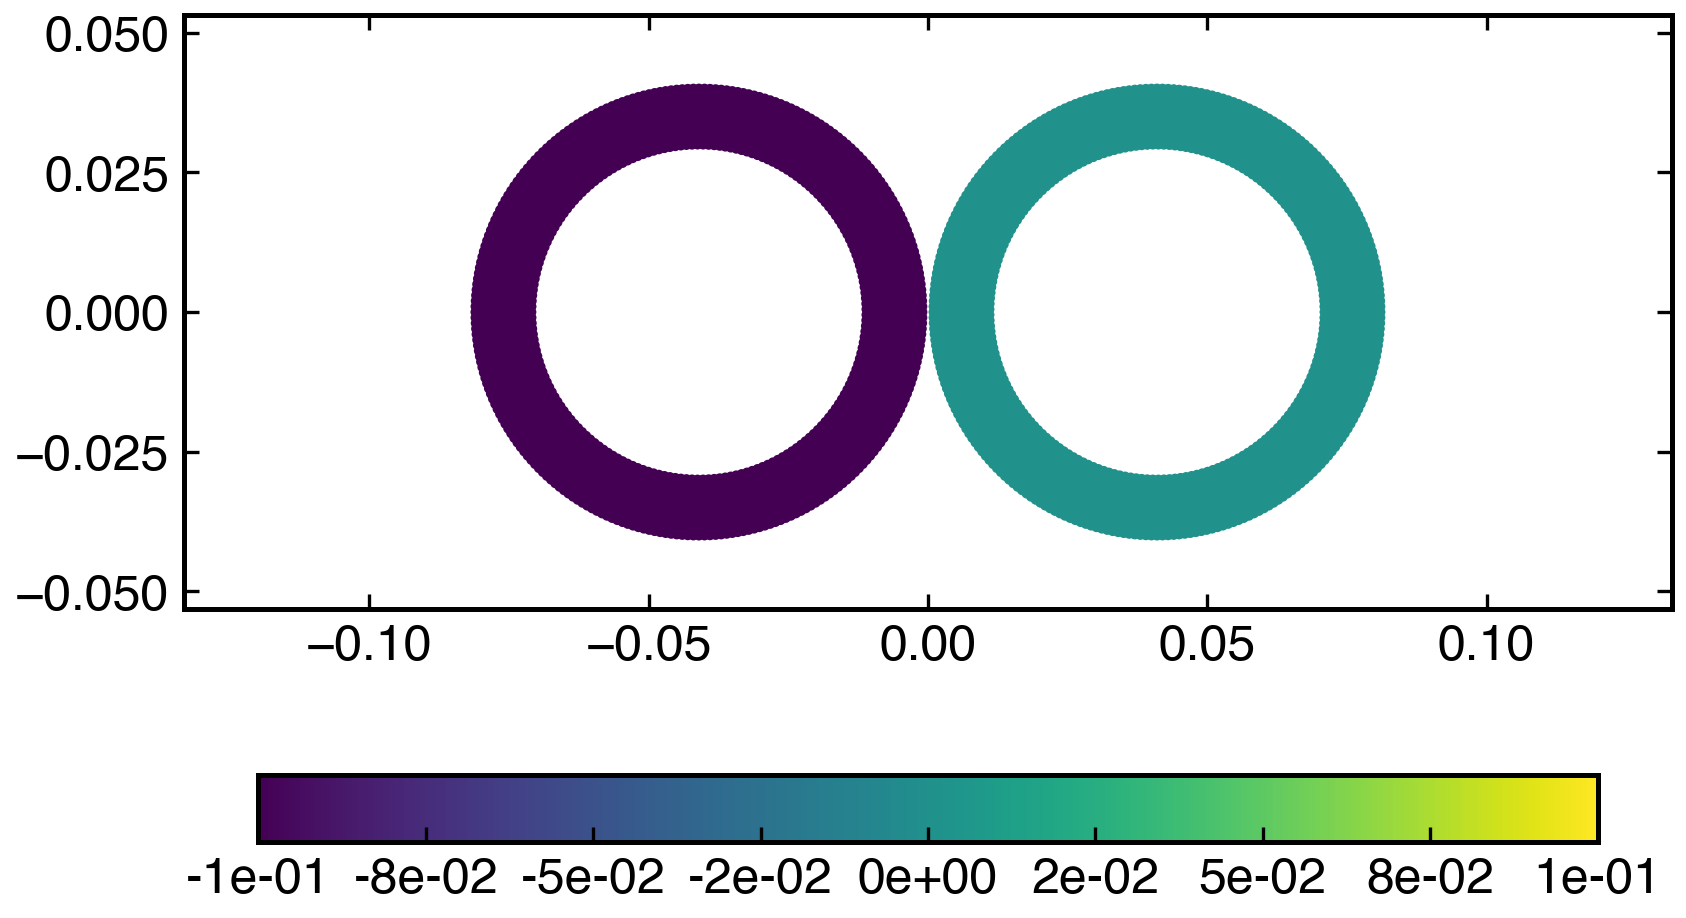
\includegraphics[width=1.0\textwidth]{figures/ctvf/figures/rings/etvf_sun2019_poisson_ratio_0.47/time0}
  %   \subcaption{t = 0 sec}\label{fig:rings:sun2019-nu-0.47-0}
  % \end{subfigure}
  %
  \begin{subfigure}{0.48\textwidth}
    \centering
    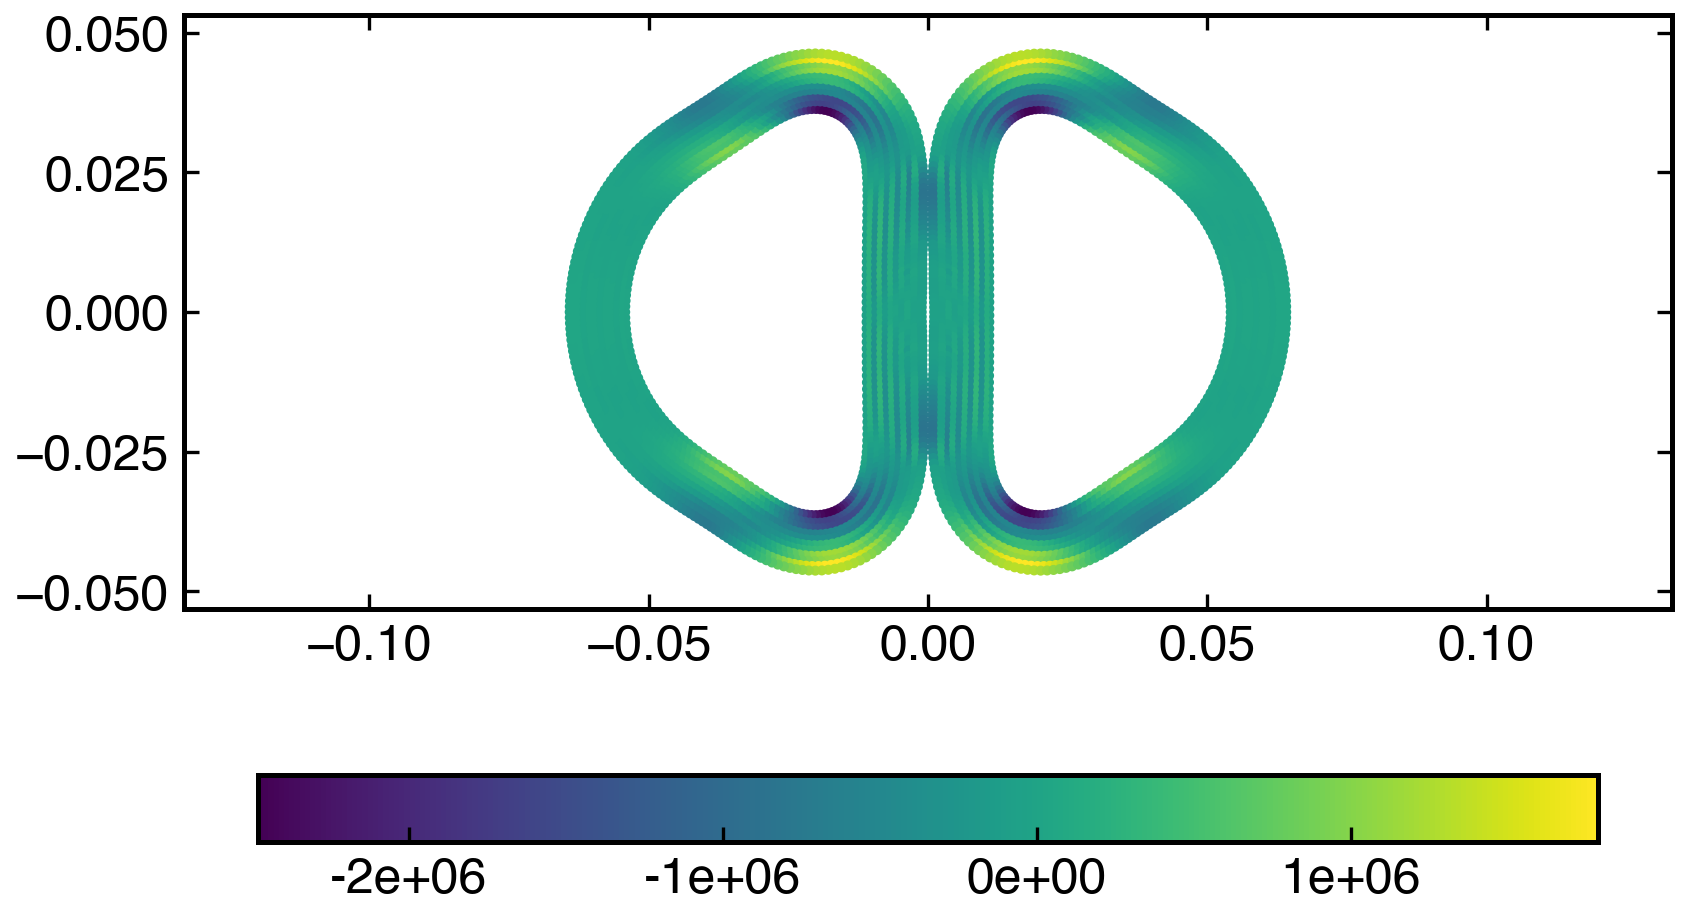
\includegraphics[width=1.0\textwidth]{figures/ctvf/figures/rings/etvf_sun2019_poisson_ratio_0.47/time1}
    \subcaption{t = 2.5e-03 sec}\label{fig:rings:sun2019-nu-0.47-1}
  \end{subfigure}
  %
  \begin{subfigure}{0.48\textwidth}
    \centering
    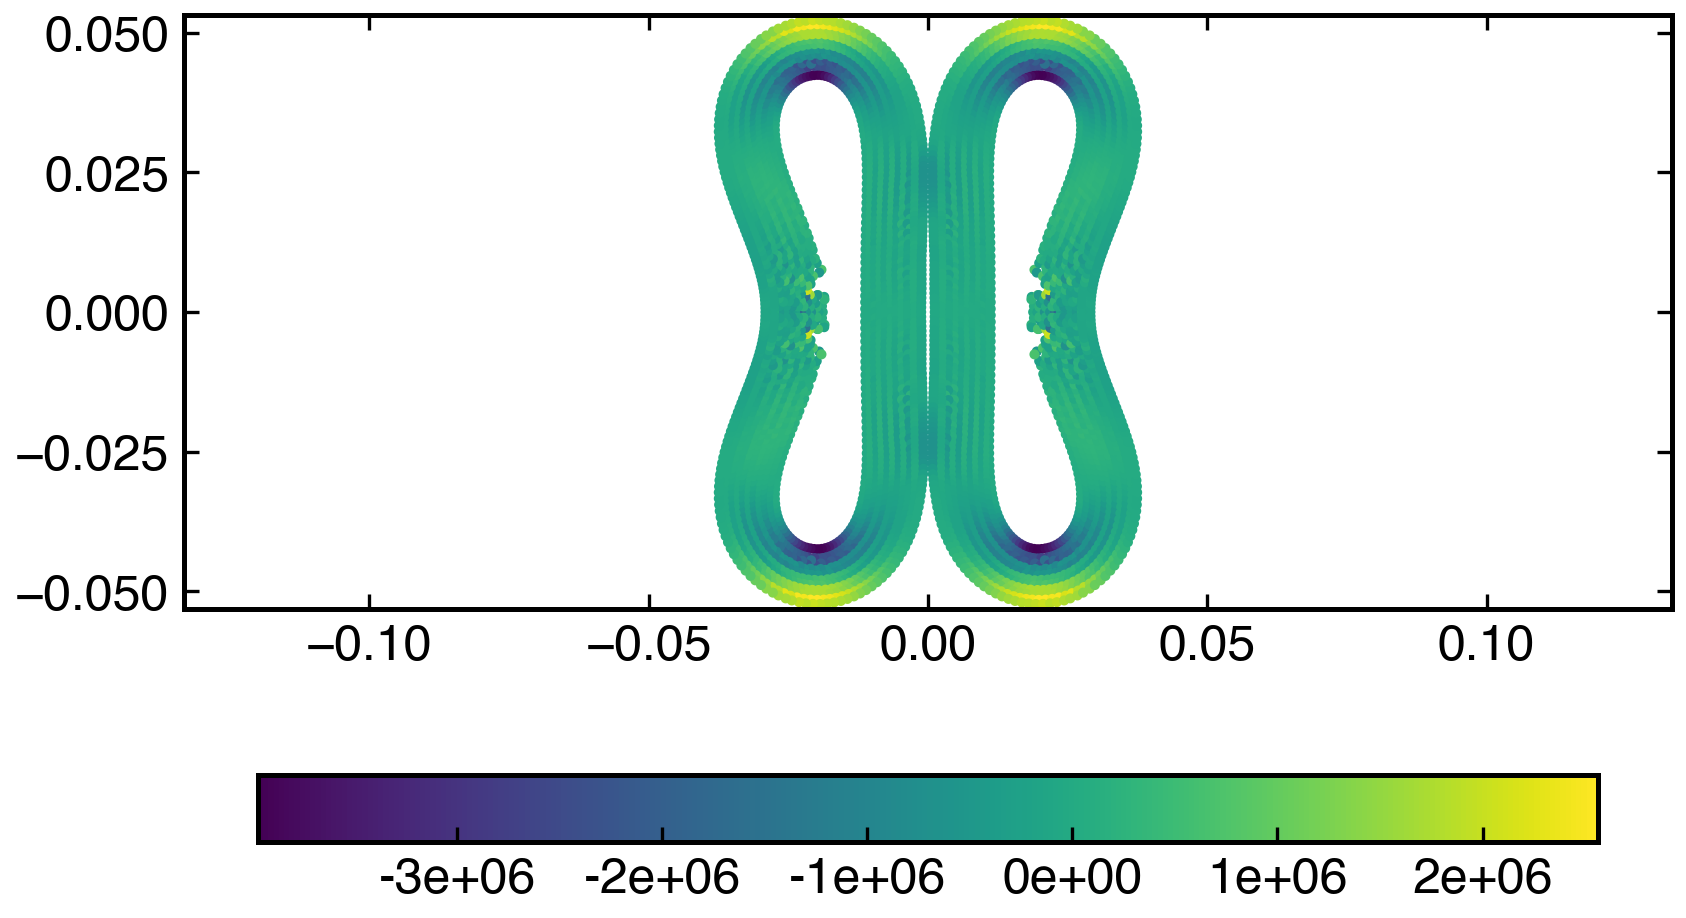
\includegraphics[width=1.0\textwidth]{figures/ctvf/figures/rings/etvf_sun2019_poisson_ratio_0.47/time2}
    \subcaption{t = 4e-03 sec}\label{fig:rings:sun2019-nu-0.47-2}
  \end{subfigure}

  \begin{subfigure}{0.48\textwidth}
    \centering
    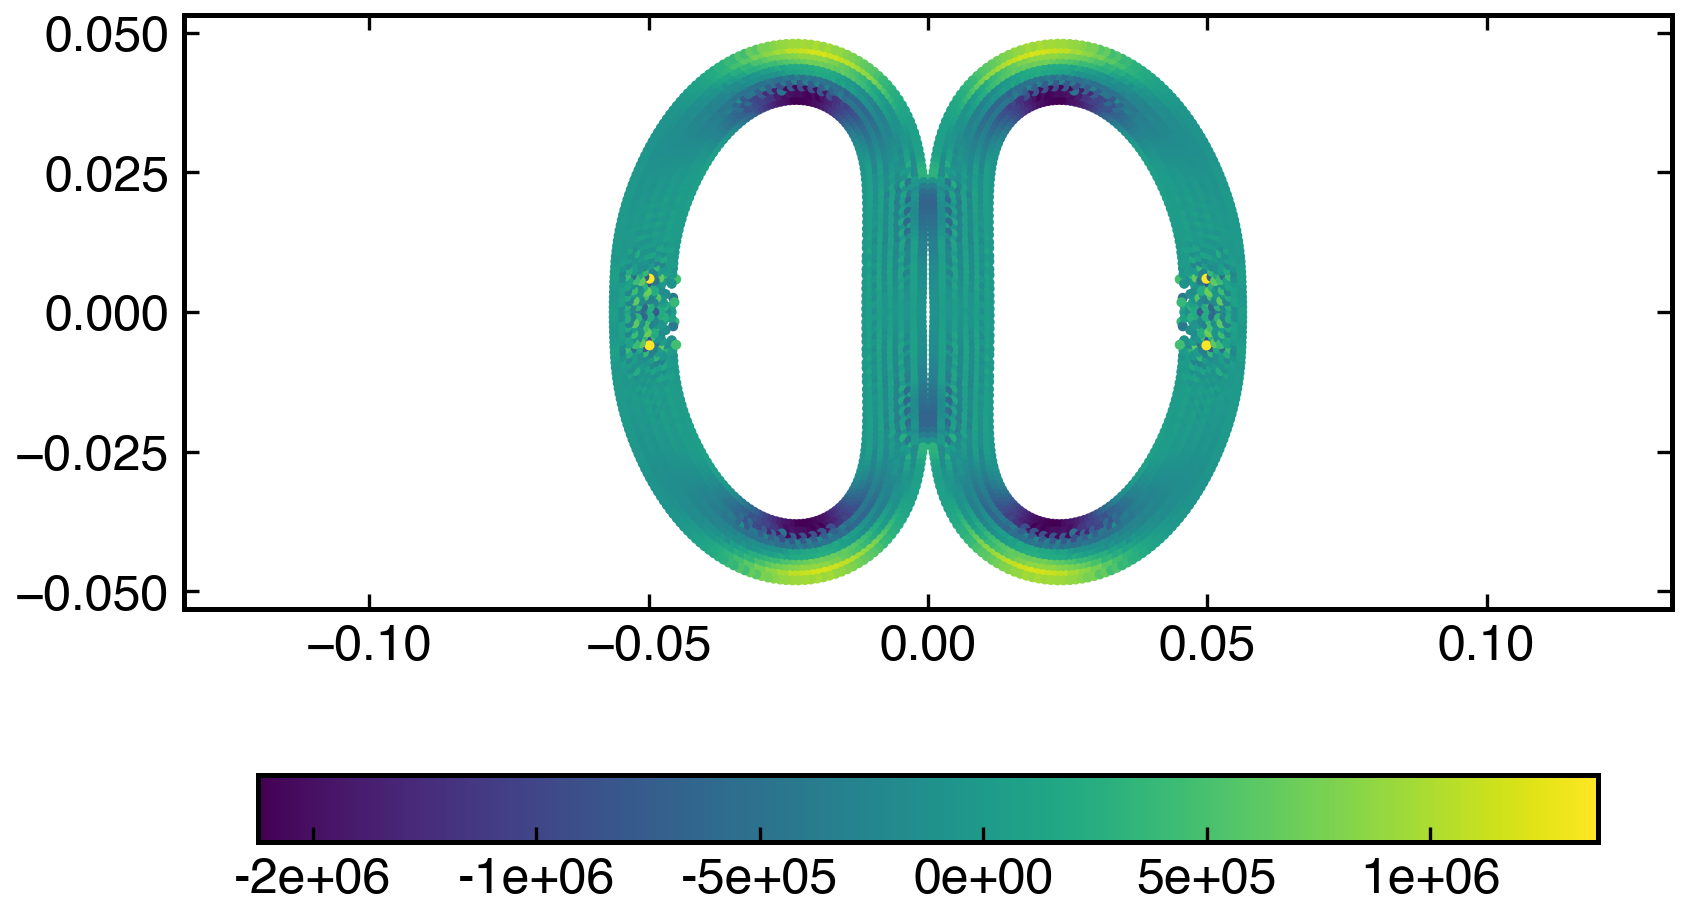
\includegraphics[width=1.0\textwidth]{figures/ctvf/figures/rings/etvf_sun2019_poisson_ratio_0.47/time3}
    \subcaption{t = 7.3e-03 sec}\label{fig:rings:sun2019-nu-0.47-3}
  \end{subfigure}
%
  \begin{subfigure}{0.48\textwidth}
    \centering
    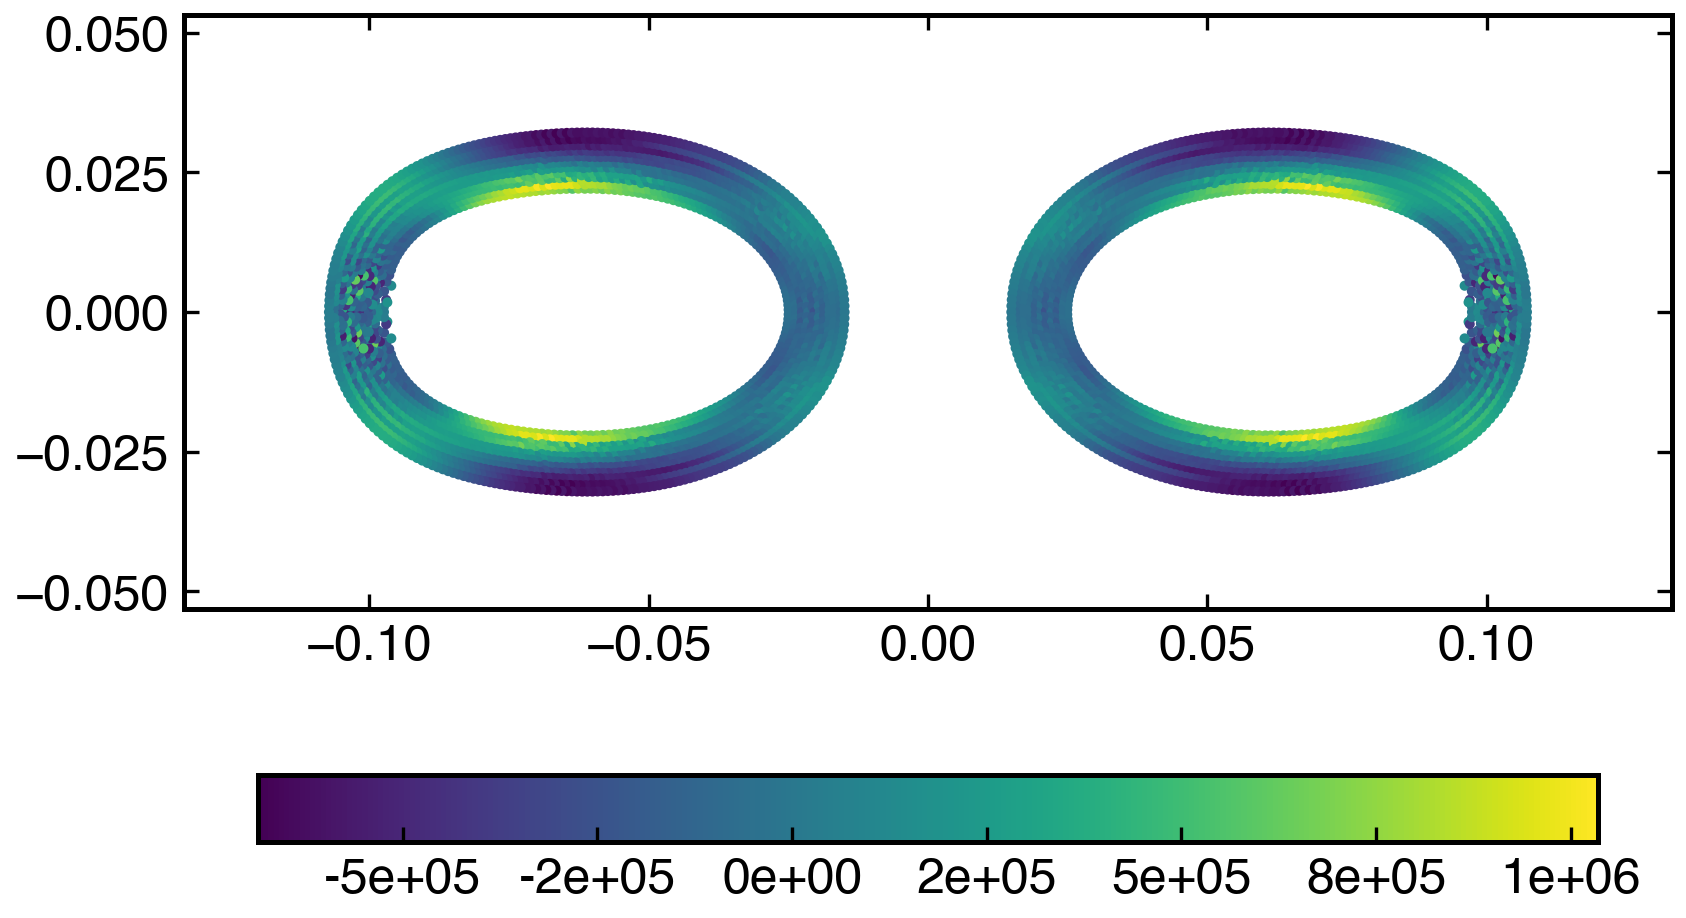
\includegraphics[width=1.0\textwidth]{figures/ctvf/figures/rings/etvf_sun2019_poisson_ratio_0.47/time4}
    \subcaption{t = 1.45e-02 sec}\label{fig:rings:sun2019-nu-0.47-4}
  \end{subfigure}
  %
%   \begin{subfigure}{0.3\textwidth}
%     \centering
%     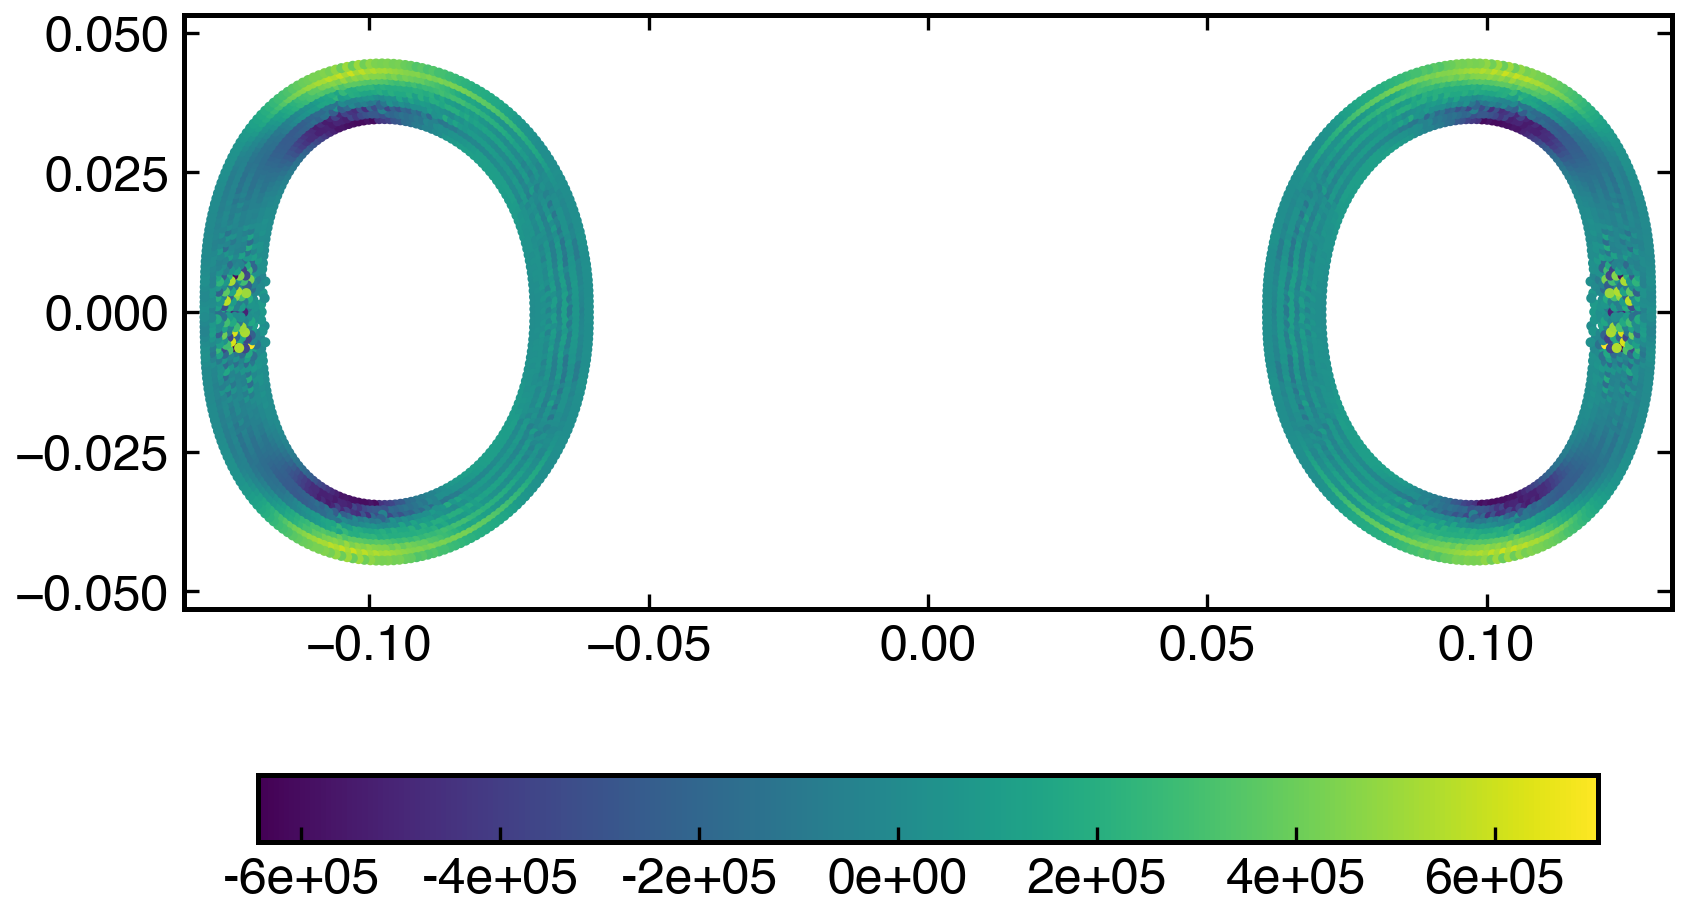
\includegraphics[width=1.0\textwidth]{figures/ctvf/figures/rings/etvf_sun2019_poisson_ratio_0.47/time5}
%     \subcaption{t = 1.5e-02 sec}\label{fig:rings:sun2019-nu-0.47-5}
%   \end{subfigure}
  \caption{Rings with a Poisson ratio of 0.47 colliding head on, simulated with CTVF using SPST.}
\label{fig:rings:sun2019-nu-0-47}
\end{figure}
%
%
\begin{figure}
  \centering
  % \begin{subfigure}{0.3\textwidth}
  %   \centering
  %   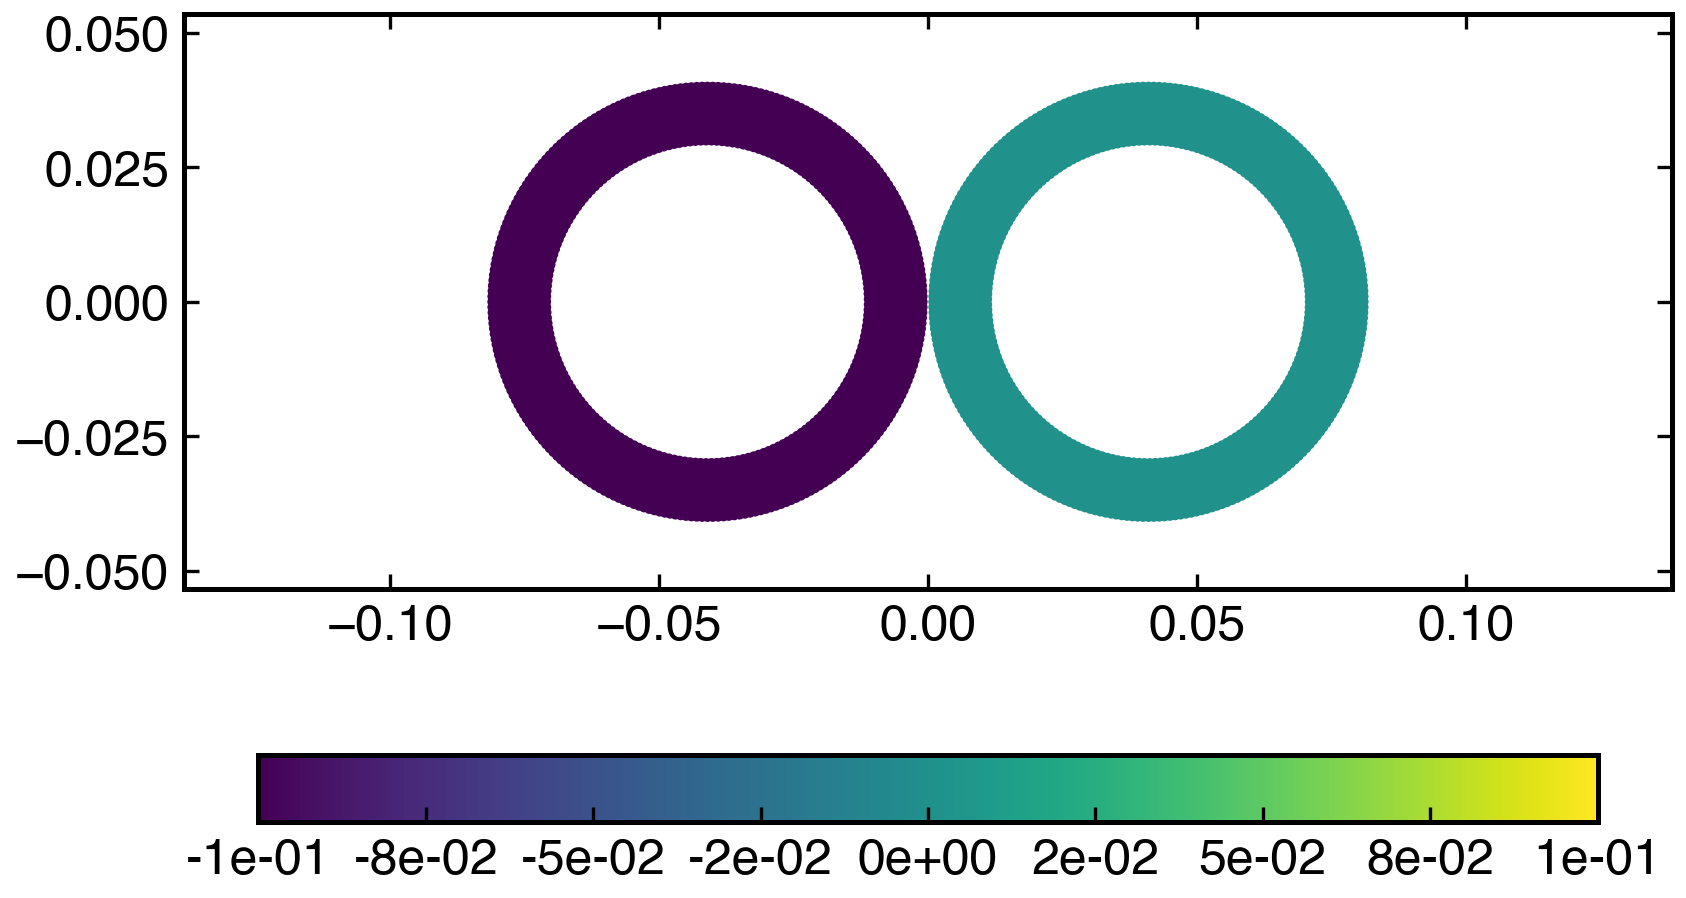
\includegraphics[width=1.0\textwidth]{figures/ctvf/figures/rings/etvf_ipst_poisson_ratio_0.47/time0}
  %   \subcaption{t = 0 sec}\label{fig:rings:ipst-nu-0.47-0}
  % \end{subfigure}
  %
  \begin{subfigure}{0.48\textwidth}
    \centering
    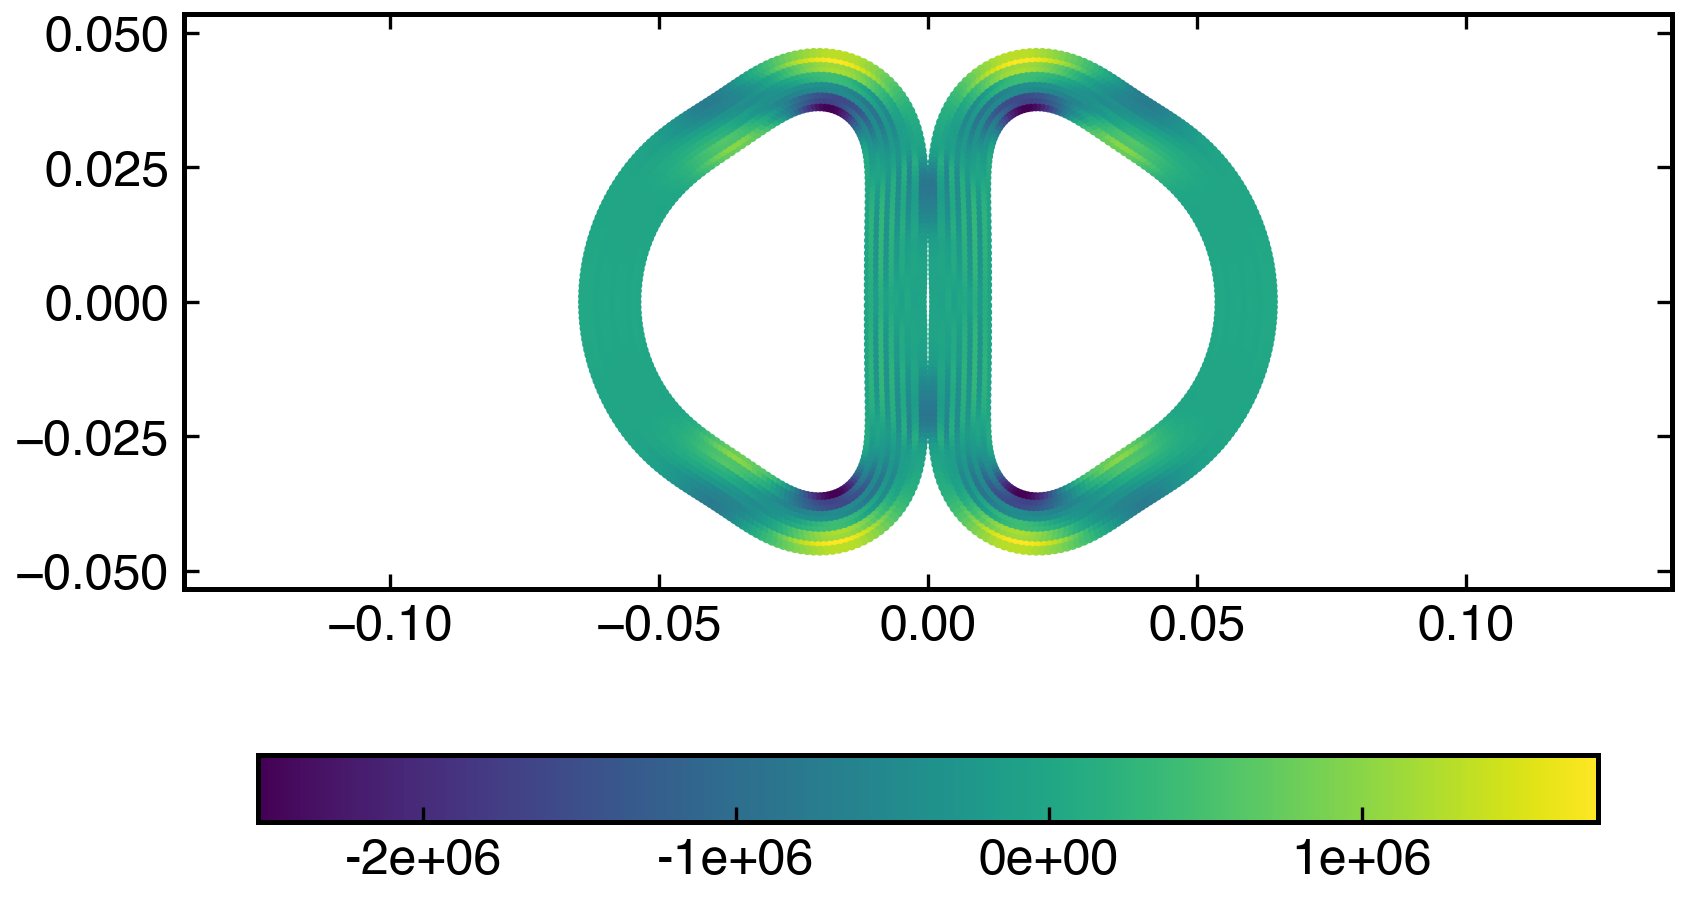
\includegraphics[width=1.0\textwidth]{figures/ctvf/figures/rings/etvf_ipst_poisson_ratio_0.47/time1}
    \subcaption{t = 2.5e-03 sec}\label{fig:rings:ipst-nu-0.47-1}
  \end{subfigure}
  %
  \begin{subfigure}{0.48\textwidth}
    \centering
    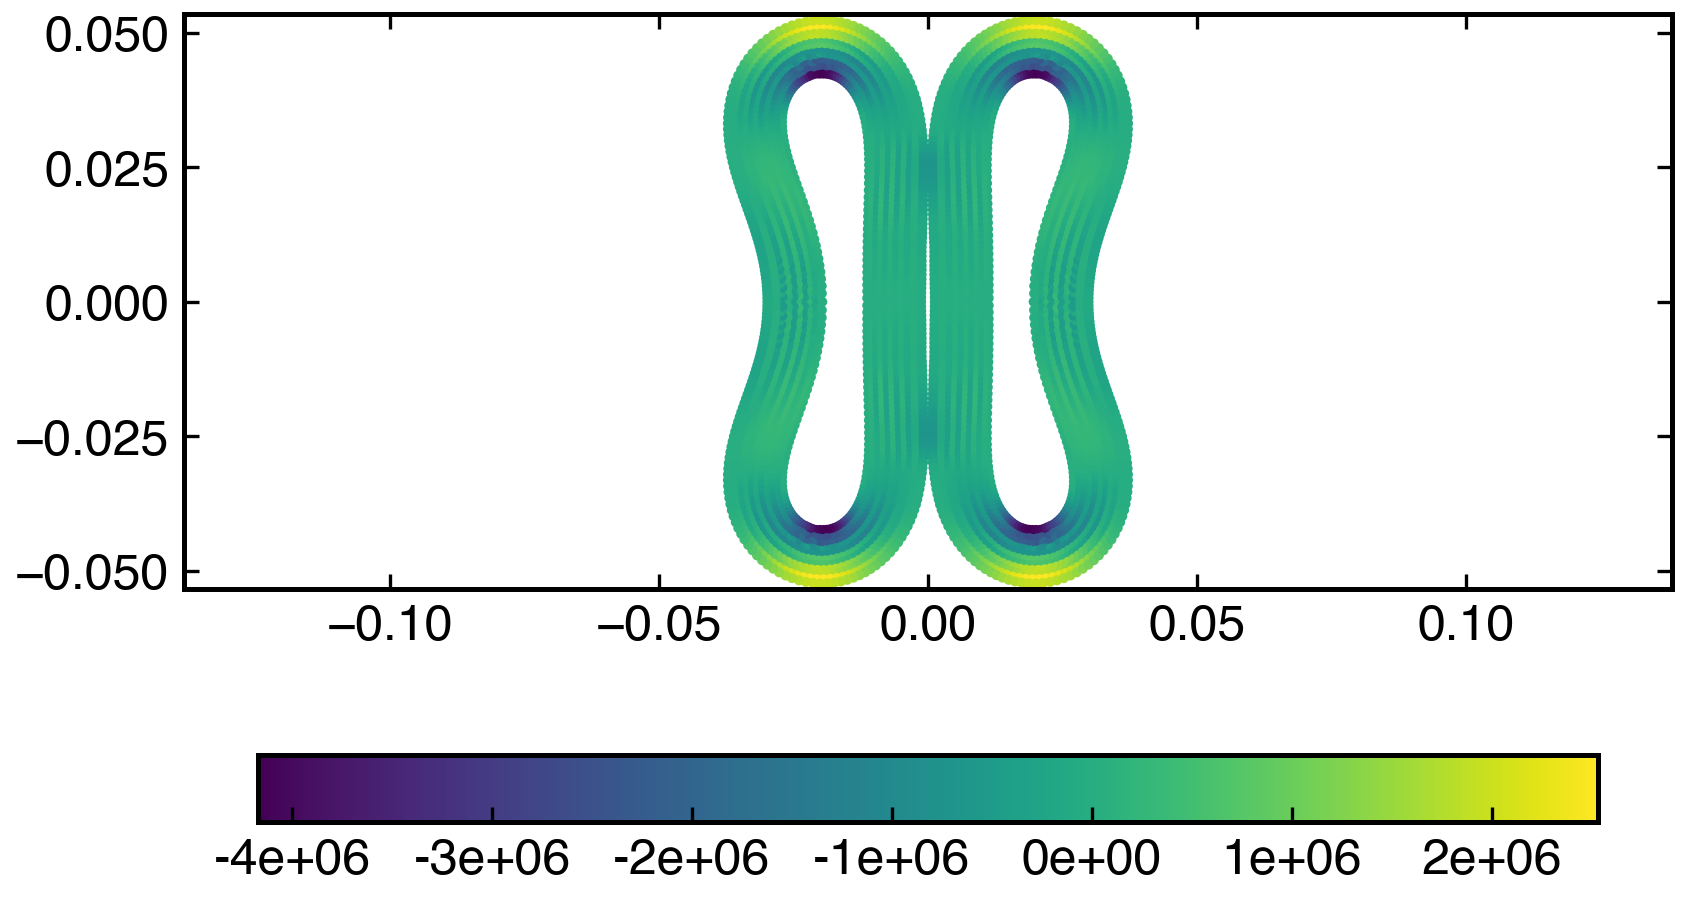
\includegraphics[width=1.0\textwidth]{figures/ctvf/figures/rings/etvf_ipst_poisson_ratio_0.47/time2}
    \subcaption{t = 4e-03 sec}\label{fig:rings:ipst-nu-0.47-2}
  \end{subfigure}

  \begin{subfigure}{0.48\textwidth}
    \centering
    \includegraphics[width=1.0\textwidth]{figures/ctvf/figures/rings/etvf_ipst_poisson_ratio_0.47/time3}
    \subcaption{t = 7.3e-03 sec}\label{fig:rings:ipst-nu-0.47-3}
  \end{subfigure}
%
  \begin{subfigure}{0.48\textwidth}
    \centering
    \includegraphics[width=1.0\textwidth]{figures/ctvf/figures/rings/etvf_ipst_poisson_ratio_0.47/time4}
    \subcaption{t = 1.45e-02 sec}\label{fig:rings:ipst-nu-0.47-4}
  \end{subfigure}
  %
  % \begin{subfigure}{0.3\textwidth}
  %   \centering
  %   \includegraphics[width=1.0\textwidth]{figures/ctvf/figures/rings/etvf_ipst_poisson_ratio_0.47/time5}
  %   \subcaption{t = 1.5e-02 sec}\label{fig:rings:ipst-nu-0.47-5}
  % \end{subfigure}
  \caption{Rings with a Poisson ratio of 0.47 colliding head on, simulated with CTVF using IPST.}
\label{fig:rings:ipst-nu-0-47}
\end{figure}
%
%
In order to compare the different schemes quantitatively for this problem, we
plot the $x$ and $y$ positions of the point A of the left ring, as can be seen
in \cref{fig:rings_initial}. \Cref{fig:rings_compare} shows the results and as
can be seen excellent agreement of the different methods for this
problem.

%
%
\begin{figure}
  \centering
  \includegraphics[width=0.4\textwidth]{images/ctvf/images/rings/rings_initial}
  \caption{Schematic diagram of two rings colliding. Points A and B are marked.}
\label{fig:rings_initial}
\end{figure}

\begin{figure}
  \centering
  \begin{subfigure}{0.48\textwidth}
    \centering
    \includegraphics[width=1.0\textwidth]{figures/ctvf/figures/rings/sun_vs_ipst_vs_gray_a_b_0_3975_x}
    \subcaption{$x$ coordinate of the point A}\label{fig:rings-compare-x}
  \end{subfigure}
  %
  \begin{subfigure}{0.48\textwidth}
    \centering
    \includegraphics[width=1.0\textwidth]{figures/ctvf/figures/rings/sun_vs_ipst_vs_gray_a_b_0_3975_y}
    \subcaption{$y$ coordinate of the point A}\label{fig:rings-compare-y}
  \end{subfigure}
  \caption{The evolution of the $x$ and $y$ coordinates of points A and B for
    the CTVF using SPST, IPST, and compared with that of
    Gray~\citep{gray-ed-2001}.}
\label{fig:rings_compare}
\end{figure}


\FloatBarrier%
\subsection{High Velocity Impact}

High-velocity impact problems are important in various contexts like space
debris applications. This case tests if the scheme is capable of hand large
deformation problems.

The projectile and the target are made of aluminium material. The projectile
is 10mm in diameter and the rectangular target has a size of $2 \times 50$ mm.
The projectile and the target have the following material properties: density
$\rho = 2785 $ kg\,m\textsuperscript{-3}, sound speed $c_0 = 5328$
 m\,s\textsuperscript{-1}, shear modulus $G=2.76 \times 10^{7}$ kPa, yield modulus
$Y_0 = 3.0 \times 10^{5}$ kPa, as studied in~\citep{zhang_hu_adams17}. The impact velocity is set to
$V_0 = 3100.0$m\,s\textsuperscript{-1}. The initial particle spacing is
$\Delta x = 0.5$ mm.
\begin{figure}
  \centering
  \begin{subfigure}{0.3\textwidth}
    \centering
    \includegraphics[width=1.0\textwidth]{figures/ctvf/figures/high_velocity_impact/etvf_sun2019/time0}
    \subcaption{t = 0 sec}\label{}
  \end{subfigure}
%
  \begin{subfigure}{0.3\textwidth}
    \centering
    \includegraphics[width=1.0\textwidth]{figures/ctvf/figures/high_velocity_impact/etvf_sun2019/time1}
    \subcaption{t = 2.5e-03 sec}\label{}
  \end{subfigure}
%
  \begin{subfigure}{0.3\textwidth}
    \centering
    \includegraphics[width=1.0\textwidth]{figures/ctvf/figures/high_velocity_impact/etvf_sun2019/time2}
    \subcaption{t = 4e-03 sec}\label{}
  \end{subfigure}

  \begin{subfigure}{0.3\textwidth}
    \centering
    \includegraphics[width=1.0\textwidth]{figures/ctvf/figures/high_velocity_impact/etvf_sun2019/time3}
    \subcaption{t = 7.3e-03 sec}\label{}
  \end{subfigure}
%
  \begin{subfigure}{0.3\textwidth}
    \centering
    \includegraphics[width=1.0\textwidth]{figures/ctvf/figures/high_velocity_impact/etvf_sun2019/time4}
    \subcaption{t = 1.45e-02 sec}\label{}
  \end{subfigure}
%
  \begin{subfigure}{0.3\textwidth}
    \centering
    \includegraphics[width=1.0\textwidth]{figures/ctvf/figures/high_velocity_impact/etvf_sun2019/time5}
    \subcaption{t = 1.5e-02 sec}\label{}
  \end{subfigure}

  \begin{subfigure}{0.3\textwidth}
    \centering
    \includegraphics[width=1.0\textwidth]{figures/ctvf/figures/high_velocity_impact/etvf_sun2019/time6}
    \subcaption{t = 1.5e-02 sec}\label{}
  \end{subfigure}
%
  \begin{subfigure}{0.3\textwidth}
    \centering
    \includegraphics[width=1.0\textwidth]{figures/ctvf/figures/high_velocity_impact/etvf_sun2019/time7}
    \subcaption{t = 1.5e-02 sec}\label{}
  \end{subfigure}
%
  \begin{subfigure}{0.3\textwidth}
    \centering
    \includegraphics[width=1.0\textwidth]{figures/ctvf/figures/high_velocity_impact/etvf_sun2019/time8}
    \subcaption{t = 1.5e-02 sec}\label{}
  \end{subfigure}
  \caption{High velocity impact of cylinder on to a structure}
\label{fig:hvi:etvf-sun2019}
\end{figure}
% start: Describe any additional physics using apart from the paper
Here the aluminium follows an elastic-perfectly plastic constitutive model. In
elastic perfectly plastic model, the material is assumed to be elastic up to
the yield point and once the material reaches the yield point, there will be
no further increase in the stress, and is bounded by a factor
$\beta = \min\left(\frac{Y_0^2}{3J_2}, 1 \right)$, where $J_2$ is calculated
from $J_2 = \frac{1}{2} \teng{\sigma}^{'} : \teng{\sigma}^{'}$. We use an
$\alpha=1$ in \cref{eq:mom-av} in the current case.

\Cref{fig:hvi:etvf-sun2019} shows the plots of cylinder impacting the
structure at different time instants. This is computed using the particle
shifting technique of Sun~\citep{sun_consistent_2019}. The color contour
represents the pressure of the particles. The width of the hole created by the
cylinder is $19.6$ mm. When computed using the GTVF
scheme~\citep{zhang_hu_adams17} the hole has a size of $19.8$ mm. In
\cite{howell2002free}, the value cited is $19.2$ mm. We can see, that the
current scheme is closer to the one simulated by \citep{howell2002free}, which
is taken as reference in \citep{zhang_hu_adams17}.


\section{Discussion}

The proposed CTVF scheme builds on the original TVF scheme of
\cite{Adami2013} and is as an improvement on the GTVF of
\cite{zhang_hu_adams17}. In addition it generalizes the implementation of the
EDAC-SPH method~\citep{edac-sph:cf:2019} where the TVF formulation was used for
internal flows and a separate WCSPH formulation used for fluid flows with a
free-surface. The current work proposes the addition of a few correction terms
which improve the accuracy of the method as demonstrated in the earlier
section. The addition of the terms imposes a small computational cost but
compensates through the improved accuracy. As an example, in simulating the
lid-driven cavity problem with a resolution of $50 \times 50$, the original
EDAC scheme without any of the correction terms with a one step predictor
corrector integrator takes $251$ seconds for a time of $25$ seconds, the new
scheme with a kick-drift-kick scheme takes $293$ seconds. Despite the change
of the integrator this is a small increase in the computational time. For solid
mechanics problems we consider the colliding rings problem simulated for a
total time of $0.016$ seconds. This takes $98$ seconds of time to simulate
with the full CTVF scheme, and takes $73$ seconds without the corrections (run
on Intel i5-7400, quad core machine). Free-surfaces are handled carefully.
The method produces smoother pressure fields due to the use of the EDAC
scheme. Finally the method is robust to changes in the PST method used. This
has been demonstrated using both the PST of \cite{sun_consistent_2019} and
the IPST of \cite{huang_kernel_2019}.

An important feature of the proposed scheme is that it works well in the
context of both fluid mechanics and solid mechanics. For elastic dynamics we
propose correction terms that improve the accuracy and robustness of the
method. The GTVF~\citep{zhang_hu_adams17} method fails when the PST method is
changed as demonstrated in \cref{sec:oscillating-plate}, however the proposed
method is more robust. Furthermore, our method uses the true velocity in order
to compute the velocity gradient. The results of the uniaxial compression
problem in \cref{sec:uniaxial-compression} suggest that that the proposed
method is more accurate than the GTVF. The main difference between the GTVF
and the current scheme in the context of solid mechanics is the addition of
the correction terms to the continuity equation, the usage of momentum
velocity $\ten{u}$ in the computation of the velocity gradient, and the new
particle shifting technique incorporation. We have found that the additional
terms arising in the equation for the Jaumann stress rate
\cref{eq:jaumann-stress-rate} has negligible influence and can be safely
ignored. However, the computations in this work have included this term. The
additional stress term in the momentum equation is negligible and has not been
employed. We reiterate that for the fluid mechanics simulations the additional
stress terms in the momentum equation are not negligible.

We note that for solid mechanics problems the method works well with either
the traditional state equation used for the pressure evolution or the use of
the EDAC equation. This does not make a significant difference for these
problems since there is no additional damping added to the evolution equation
for the deviatoric stresses. The EDAC evolution equation does make a
significant improvement to the pressure evolution in the fluid mechanics
problems as discussed earlier in \citep{edac-sph:cf:2019}.

The newly proposed method has not been applied to three dimensional problems
or to fluid structure interaction (FSI) problems. We believe that the method
would be easier to use in the context of FSI since it can handle both fluids
and solids in the same formulation. We propose to investigate these in the
future.


In the current chapter, we have developed a transport velocity formulation-based
method in SPH to solve fluid and solid dynamics problems. The developed method
is robust and is able to eliminate several issues raised in conventional SPH. We
have an updated Lagrangian solver with reasonable fidelity, which can solve
fluid and elastic problems. As part of developing a framework to model complex
physical processes, we can couple the improved technique to handle various
multiphysics problems in water jet machining. In the next chapter, we will model
the collision among impacting bodies when they are assumed as elastic. We will
extend the current solver to handle the collision between the elastic solids,
where the collision is dealt with a contact force using the boundary particles.
Using a contact force model, we will eliminate various issues SPH faces while
handling the collision of elastic objects, and additionally, we will incorporate
friction between the colliding bodies.

\chapter{Collision SPH}
\label{chap:csph}



\section{Introduction}
\label{sec:intro}
In the current chapter we model the collision between elastic bodies. Modeling
the collision among elastic solids allows us to handle the interaction between
the target and the impactor when they are assumed as elastic or elastic-plastic.
An SPH based solution leads to unphysical interactions in modeling the collision
of objects when they are close by but not touching. Further, SPH model does not
incorporate friction between the colliding bodies. In the current chapter, a
contact force model is incorporated into the existing solver to handle the
interaction between the colliding solids. Specifically, we consider bodies with
arbitrary shapes.


The collision of arbitrary solid bodies occurs everywhere around us. Apart
from the elastic collision of bodies, other important examples include surface
erosion, waterjet machining \parencite{natarajan2020abrasive}, and machining
processes \parencite{islam2020numerical} to note a few. It is important to be able
to simulate such problems accurately.

% When body A discretized into n particles is colliding a body B which is
% discretized in to m particles, above techniques use the particles in B to
% compute the accelerations of density and velocity of particles in A. A few
% drawbacks of this approach is, the bodies come in to contact even when the
% bodies are physically not touching, and the no frictional modeling is modeled.
% \textcite{yan2021simulation} has proposed a interfacial SPH scheme , where each
% elastic body uses their own particles in computation of divergence, momentum
% and strain rate. While, the bodies interact by a repulsive force inspired from
% Ansys. Where they have shown the improvement on modeling the collision with
% different examples. Yan has considered Gray SPH which is not so great with
% kernel invariance as it shows tensile instability with a few kernels as shown
% by Roth 2020. Also the contact force model didn't incorporate the frictional
% part of the collision. Further the contact force has a influence of 2h radius,
% implies there would be a force acting on the interacting bodies though they
% are not touching physically.

% The contact force model used in Yan is inspired from ANSYS model and is given.
% A similar work is done by \textcite{vyas2021collisional}, where the author models
% the interaction between a circular rigid body impacting a target surface. In
% his work, author proposes a non-linear penalty based force model which could
% handle friction as well and studies the rebounding characteristic of the
% impactor. Here, the author studies the post collision behaviour of the
% circular rigid body which is interacting the elastic plastic solid at
% different incident angles. \textcite{mohseni2021particle} proposed an advanced
% version of the collision model where he models the interaction between a rigid
% body with a brittle solids and models the erosion of the brittle solid.

% Finally the current model comes into place only when the material interfaces
% are touching unlike what Yan's contact force model and conventional SPH. We
% also check the invariance of the current scheme in modeling the collisions for
% different types of kernels used.


In the current work, the collision between elastic solids is modeled using a
penalty-based contact force model. A contact force based approach for collision
handling will eliminate the spurious interaction between bodies, which occurs
while modeling with an SPH-based model. We address the importance of choosing
the primary and secondary body. The work of \textcite{mohseni2021particle} takes
inspiration from that of \textcite{vyas2021collisional} where too there is a clear
distinction between primary and secondary bodies. \textcite{vyas2021collisional}
also consider the collision between a rigid and elastic body. In the present
work we only implement the collision model of \parencite{mohseni2021particle} due to
its simplicity. The model proposed by \textcite{vyas2021collisional} is more complex
to implement. Several examples are simulated to validate the current scheme,
ranging from simulations compared with FEM, analytical results as well as
experimental. We next look at the numerical method used to model the collision
among the elastic solids.


\FloatBarrier%
\section{SPH Model for Structural Dynamics}
\label{sec:SPH-model-for-structural-dynamics}
In this section, we discuss the formulation of collision SPH.
\subsection{Discrete Governing Equations}
\label{sec:discrete-governing-equations}
We follow the CTVF formulation developed in \cref{chap:ctvf} to handle the
structural dynamics of the solid. The governing equations of including the new
contact force term are:
\begin{equation}
\label{eqn:sph-continuity}
  \frac{\tilde{d}\rho_a}{dt} = \sum_{b \in A} \; \frac{m_b}{\rho_{b}} \; (
  \rho_{a} \; \tilde{\ten{u}}_{ab} \; + \;
  (\rho \; (\tilde{\ten{u}} \; - \;
  \ten{u}))_{ab}) \; \cdot \nabla_{a} W_{ab},
\end{equation}
\begin{equation}
\label{eqn:sph-momentum}
  \frac{\tilde{d}\ten{u}_{a}}{dt} = - \sum_{b \in A} m_b \bigg[
  \bigg(\frac{p_a}{\rho_a^2} + \frac{p_b}{\rho_b^2}\bigg) \ten{I} -
  \bigg(\frac{\teng{\sigma}^{'}_{a}}{\rho_a^2} +
  \frac{\teng{\sigma}^{'}_{b}}{\rho_b^2} + \Pi_{ab} \ten{I} \bigg) \bigg]  \cdot \nabla_{a} W_{ab} +
  \ten{g}_{a} + \frac{1}{m_a}\sum_{b \in B} \ten{F}^{\text{cont}}_{a \leftarrow b}.
\end{equation}
Here, $\ten{F}^{cont}_{a}$ is the force acting on particle $a$ due to
\begin{figure}[!htpb]
  \centering
  \includegraphics[width=1.0\textwidth]{images/csph/images/contact_force/contact_force_description}
  \caption{Bodies under collision which are divided into primary and
    secondary.}
\label{fig:bodies_under_collision}
\end{figure}
contact with the other elastic bodies which will be discussed in
\cref{sec:contact-algorithm}. We follow \cref{chap:ctvf} in handling the
boundaries, updating the state of the bodies, to compute the transport velocity
of the particles.


\FloatBarrier%
\section{Contact Algorithm}
\label{sec:contact-algorithm}
In the current work we have utilized the contact force model proposed by
\textcite{mohseni2021particle}. The force acting on a particle $a$ of body A due
to the interaction with the particles of body $B$ can be resolved into a
normal and tangential component. The normal force component is utilised to
make sure that the particles of different bodies do not penetrate into each
other, while the tangential component is used to model the friction between
the interacting solids. According to \textcite{mohseni2021particle}, we divide the
bodies under interaction into primary and secondary bodies, as shown in
\cref{fig:bodies_under_collision}.
% In usual DEM to compute the force on particle i of body A, the force is
% computed by considering the overlap of particle i with each and every
% particle of body j by considering the particle j to be spherical. This leads
% to unphysical modeling of contact force when the body is interacting with a
% flat surface or surfaces which are not spherical by nature. The current
% contact force is surface aware. The force on particle $i$ is computed by
% equation
The normal force ($\teng{F}_a^{n}$) on
particle $a$ due to the interaction with the particles $b$ of body $B$ is
computed as,
\begin{equation}
  \label{eq:contact-algorithm-normal}
  \ten{F}_a^n = k_r \delta_{n^{c}}^{a} \ten{n}_a^{c}.
\end{equation}
Here, the overlap $\delta_{n^{c}}^{a}$ is computed using
\begin{equation}
  \label{eq:csph:cf-overlap}
  \delta_{n^{c}}^{a} = \Delta x - d_a,
\end{equation}
where,
\begin{equation}
  \label{eq:cf-distance-computation}
  d_a = \frac{
    \displaystyle\sum\limits_{b = 1}^{\text{NP}^{b}} \;
    \big( \ten{n}_a^{c} \cdot \ten{r}_{ab} \big)  \frac{m_b}{\rho_b} W_{ab}}
  {
    \displaystyle\sum\limits_{b = 1}^{\text{NP}^{b}} \;
    \frac{m_b}{\rho_b} W_{ab}},
\end{equation}
and the normal contact vector $\ten{n}_a^{c}$ is computed using
\begin{equation}
  \label{eq:cf-normal-vector}
  \ten{\hat{n}}_a^{c} = \frac{
    \displaystyle\sum\limits_{b = 1}^{\text{NP}^{b}} \;
    \frac{\ten{r}_{ab}}{r_{ab}}  \frac{m_b}{\rho_b} W_{ab}}
  {
    \displaystyle\sum\limits_{b = 1}^{\text{NP}^{b}} \;
    \frac{m_b}{\rho_b} W_{ab}},
\end{equation}
\begin{equation}
  \label{eq:cf-normal-vector}
  \ten{n}_a^{c} = \frac{\teng{\hat{n}}_a^{c}}{||\teng{\hat{n}}_a^{c}||}.
\end{equation}
\begin{figure}[!htpb]
  \centering
  \includegraphics[width=0.3\textwidth]{images/csph/images/contact_force/contact_force_delta_computation}
  \caption{Pictorial representation of distance between a particle and a body.}
\label{fig:contact_force_delta_computation}
\end{figure}
Where $\Delta x$ being the initial spacing between the particles, $k_r$ is the
normal spring stiffness coefficient. \Cref{fig:contact_force_delta_computation}
shows $\Delta x$ and $d_a$ quantities, respectively. Note that while computing
the overlap of particle $a$ with the body $B$ we have computed an effective
overlap, rather than per particle interaction. This is effectively able to model
the interaction between non-smooth surfaces in contrast with particle-particle
force computation.

\subsection{Tangential Force Computation}
\label{sec:tangential-force-computation}
We associate a tangential spring attached to particle $a$
($|\Delta \textit{\textbf{l}}_a|$) and body $B$ to compute the tangential force
($\ten{F}_{a}^{t}$), which initially has a magnitude of zero
($|\Delta \textit{\textbf{l}}_a|=0$). The tangential spring is activated when
the particle comes into contact with body $B$. The tangential force is
history-dependent. The contact friction force is proportional to the tangential
spring displacement, which is integrated over the contact time as
\begin{equation}
  \label{eq:tangential-force}
  \ten{F}_{a}^{t^{n+1}} =
  -k_f \Delta \textit{\textbf{l}}_a^{\,n + 1} =
  -k_f \big[\big(\Delta {\textit{\textbf{l}}}_a^{\,n} \
  + \ten{v}_{ab}^{n + 1} \Delta t\big) \cdot \ten{t}_a^{n + 1} \big] \
  \ten{t}_a^{n + 1},
\end{equation}
where $\Delta t$ is the time step, $\ten{v}_{ab} = \ten{v}_{a} - \ten{v}_b$ is
the relative velocity of the primary particle $a$ with respect to the closest
secondary particle $b$, $\ten{t}_a$ is the tangential unit vector, and $k_f$ is the tangential spring stiffness
coefficient. Here, $n$ and $n+1$ represent the times which are $\Delta t$ apart.
The tangential unit vector is computed by,
\begin{equation}
  \label{eq:tangential-vect}
  \ten{t}_a = \frac{\ten{v}_{ab} - (\ten{v}_{ab} \cdot \ten{n}_a^{c}) \ten{n}_a^{c}}{|\ten{v}_{ab} - (\ten{v}_{ab} \cdot \ten{n}_a^{c}) \ten{n}_a^{c}|}.
\end{equation}

The tangential force is coupled to the normal force through the Coulomb's law,
\begin{equation}
  \label{eq:Coulomb-law}
  \ten{F}_{a}^{t} = \min(\mu |\ten{F}_{a}^{n}|, |\ten{F}_{a}^{t}|) \
  \frac{\ten{F}_{a}^{t}}{|\ten{F}_{a}^{t}|}.
\end{equation}
This allows us to impose the sliding friction condition between the
interacting solids. Finally, the total force acting on the particle $a$ due to
the interaction with body $B$ is:
\begin{equation}
  \label{eq:contact-force}
  \ten{F}_{a}^{\text{cont}} = \ten{F}_{a}^{n} + \ten{F}_{a}^{t}
\end{equation}

\begin{figure}[!htpb]
  \centering
  \includegraphics[width=0.3\textwidth]{images/csph/images/contact_force/contact_force_description_3}
  \caption{Force transfer to the secondary particles $b$ from the primary body particle $a$}
\label{fig:secondary_particle_contact_foce_transfer}
\end{figure}
An equal and opposite force of the same magnitude is applied to the closest
secondary particle $b$ of $a$ as shown in
\cref{fig:secondary_particle_contact_foce_transfer},
\begin{equation}
  \label{eq:contact-force}
  \ten{F}_{b}^{\text{cont}} = - \ten{F}_{a}^{\text{cont}}.
\end{equation}

% The force on the particle $j$ is evaluated, on the
% body belonging to the secondary surface is as follows. Particles belonging to
% the secondary surface ($j$) which are at a distance less than the initial
% spacing ($l_0$) share the force exerted on particle i, as following:
% \begin{equation}
%   \label{eq:cf-overlap}
%   F^{ij} = - F^{i} w^{ij},
% \end{equation}
% where $w^{ij}$ is defined as
% \begin{equation}
%   \label{eq:cf-overlap}
%   w^{ij} = \frac{n^{i} \cdot \hat{\ten{r}}^{ij}}{\sum_j n^{i} \cdot \hat{\ten{r}}^{ij}}
% \end{equation}

The current contact force model is sensitive towards the primary body chosen
to compute the forces, i.e., the force acting on the particles is not the same
when the primary bodies are interchanged. In the current work we have explored
the behaviour of the current contact force model when different bodies are
chosen as primary and secondary. Simulations such as, a rectangular solid
sliding down an inclined plane, and a symmetric collision between elastic
solids are two examples, where we have investigated how the bodies would behave
when different bodies are chosen as primary.
% , as shown in \cref{fig:primary-secondary-demonstration}.
% \begin{figure}[!htpb]
%   \centering
%   \begin{subfigure}{0.48\textwidth}
%     \centering
%     \includegraphics[width=1.0\textwidth]{images/csph/images/primary_vs_secondary/sliding}
%     \subcaption{A sliding body.}%\label{fig:rings:ipst-nu-0.47-0}
%   \end{subfigure}
%   \begin{subfigure}{0.48\textwidth}
%     \centering
%     \includegraphics[width=1.0\textwidth]{images/csph/images/primary_vs_secondary/symmetric_collision}
%     \subcaption{A symmetric collision between rectangular solids.}%\label{fig:rings:ipst-nu-0.47-1}
%   \end{subfigure}
%   \caption{Examples used to explore the importance of choosing a primary.}
% \label{fig:primary-secondary-demonstration}
% \end{figure}

% =========================================== %
% ------ Results start ---------------------- %
% =========================================== %

\FloatBarrier%
\section{Results and Discussion}
\label{sec:results}
In the interest of reproducibility and easier ability
for researchers to build on this work, our code is open source and can be
found at \url{https://gitlab.com/pypr/collision_sph}. We use the
\texttt{automan} package~\parencite{automan2018} to automate all the results
generated.

\FloatBarrier%
\subsection{Curved Interface}
\label{sec:results-circular-interface}
\begin{figure}[!htpb]
  \centering
  \includegraphics[width=0.6\textwidth]{images/csph/images/yan_2021_curved_interface/schematic}
  \caption{Collision between two circular elastic discs. The left disc moves
    towards the right disc with a constant velocity $v_0$, while the right
    disc is at rest.}
\label{fig:results-yan-circular-interface-schematic}
\end{figure}
The collision of two circular elastic solids is considered as the first test
case. \Cref{fig:results-yan-circular-interface-schematic} shows the initial
configuration where the left disc is initially allowed to move towards the
right with a velocity of 20 m\,s\textsuperscript{-1}. While no velocity is
imposed on the right disc. The radius of each disk is $0.4$ m, and made of
Aluminium, whose material properties are shown in
\cref{tab:curved-interface-material-params}. No friction and gravity is
assumed in the current case. A particle spacing of 0.01 m is used, resulting
in a $4779$ particles per disc. The numerical parameters utilized in
the current example are shown in \cref{tab:curved-interface-numerical-params}.
\begin{table}[!ht]
  \centering
  \begin{tabular}[!ht]{ll}
    \toprule
    Quantity & Values\\
    \midrule
    $E$, Young's modulus & $72$ GPa \\
    $\nu$, Poisson's ratio & $0.3$ \\
    $\rho$, density & $2785$ kg\,m\textsuperscript{-3} \\
    $\mu$, friction coefficient & $0$ \\
    Time of simulation & $4$ ms \\
    gravity $[g_x, g_y, g_z]$ & $[0.0, 0.0, 0.0]$\\
    \bottomrule
  \end{tabular}
  \caption{Material parameters used for the impact of curved interface problem.}%
  \label{tab:curved-interface-material-params}
\end{table}
\begin{table}[!ht]
  \centering
  \begin{tabular}[!ht]{ll}
    \toprule
    Quantity & Values\\
    \midrule
    $\delta x $, Resolution & $0.01$\\
    $h/\Delta x$, Smoothing length factor & 1\\
    $\alpha$, artificial viscosity & $1$ \\
    $\beta$, artificial viscosity & $0$ \\
    $k_r$, Normal stiffness coefficient & $10^{10}$ \\
    $k_f$, Tangential stiffness coefficient & $10^{9}$ \\
    \bottomrule
  \end{tabular}
  \caption{Numerical parameters used for the impact of curved interface problem.}%
  \label{tab:curved-interface-numerical-params}
\end{table}

\Cref{fig:yan-2021-curved:improved-ipst-nu-0-47} shows the snapshots of
particles of the circular disc under contact by the present approach including
the stress ($\sigma_{xx}$) field at times $t=0.0, 1.8, 4$ ms. From the figure,
we can see that the current numerical scheme is able to reproduce smooth
stress fields. The elastic discs are initially in stress free state, and once
the bodies collide, the left disc transfers its momentum to the right. Since
the discs are elastic, the total momentum is not transferred, and the left
disc will not come to a halt but rather starts moving with the free vibration
of the disc.
\begin{figure}[!htpb]
  \centering
  \begin{subfigure}{0.48\textwidth}
    \centering
    \includegraphics[width=1.0\textwidth]{figures/csph/figures/yan_2021_curved_interface/collision_ctvf/time0}
    \subcaption{t = $0$ ms}\label{fig:rings:ipst-nu-0.47-0}
  \end{subfigure}
  \begin{subfigure}{0.48\textwidth}
    \centering
    \includegraphics[width=1.0\textwidth]{figures/csph/figures/yan_2021_curved_interface/collision_ctvf/time1}
    \subcaption{t = $1.8$ ms}\label{fig:rings:ipst-nu-0.47-1}
  \end{subfigure}

  \begin{subfigure}{0.48\textwidth}
    \centering
    \includegraphics[width=1.0\textwidth]{figures/csph/figures/yan_2021_curved_interface/collision_ctvf/time2}
    \subcaption{t = $4$ ms}\label{fig:rings:ipst-nu-0.47-2}
  \end{subfigure}
  \caption{The stress field of the elastic discs at three different time
    instants through the collision.}
\label{fig:yan-2021-curved:improved-ipst-nu-0-47}
\end{figure}

\Cref{fig:results-yan-curved-velocity-vs-time} presents the time histories of
the velocity of the center of mass of both the discs in comparison with the
results by FEM solver presented in \parencite{yan2021simulation}. The rebound the
velocity of the bodies with the current scheme is in good match with the FEM
result.
% \todoin{Add why CTVF is different}
\begin{figure}[!htpb]
  \centering
  \includegraphics[width=0.6\textwidth]{figures/csph/figures/yan_2021_curved_interface/velocity_vs_time}
  \caption{Time history of the x component of velocity of center of mass's of
    the left and the right disc, and compared with the numerical results
    produced using FEM, CTVF. The Young's modulus of the disc is taken as
    $E$=$72$ GPa.}
\label{fig:results-yan-curved-velocity-vs-time}
\end{figure}

We check if the elastic disk behave as a rigid disk with an increase in
Young's modulus and is able to retrieve the rigid velocity. We expect the
right disk to achieve the velocity of $20$ m\,s\textsuperscript{-1} as the
Young's modulus is increased. \Cref{fig:results-yan-curved-E-vs-velocity}
shows the variation of the final velocity of the right disc with Young's
modulus, where we can see that the proposed model is behaving as expected.
\begin{figure}[!htpb]
  \centering
  \includegraphics[width=0.6\textwidth]{figures/csph/figures/yan_2021_curved_interface/E_vs_velocity}
  \caption{Variation of the x-velocity of the center of mass with Young's
    modulus of the disc.}
\label{fig:results-yan-curved-E-vs-velocity}
\end{figure}

% ===================================================
% ===================================================
\FloatBarrier%
\subsection{Flat Interface}
\label{sec:results-linear-interface}
In the current section, we test our solver in handling collision between two
elastic solids, where the collision front is flat in shape. The model is
shown in \cref{fig:results-yan-linear-interface-schematic}. Both the solids
are of the same size, $0.2$ m in length and $0.1$ m in height. The material is
the same as in the circular interface problem
(\cref{sec:results-circular-interface}) and can be found in
\cref{tab:curved-interface-material-params}, while the numerical parameters
are listed in \cref{tab:linear-interface-numerical-params}. A particle spacing
of $0.0025$ m is used, resulting in $3321$ particles per body.
\begin{figure}[!htpb]
  \centering
  \includegraphics[width=0.8\textwidth]{images/csph/images/yan_2021_linear_interface/schematic}
  \caption{
    Collision between two rectangular elastic solids, where, the left solid is allowed
    to move towards the right solid with a constant velocity $v_0$, while the right
    solid is at rest.}
\label{fig:results-yan-linear-interface-schematic}
\end{figure}
\begin{table}[!ht]
  \centering
  \begin{tabular}[!ht]{ll}
    \toprule
    Quantity & Values\\
    \midrule
    $h/\Delta x$, Smoothing length factor & 1\\
    $\alpha$, artificial viscosity & $1$ \\
    $\beta$, artificial viscosity & $0$ \\
    $k_r$, Normal stiffness coefficient & $10^{11}$ \\
    $k_f$, Tangential stiffness coefficient & $10^{9}$ \\
    \bottomrule
  \end{tabular}
  \caption{Numerical parameters used for the impact of linear interface problem.}%
  \label{tab:linear-interface-numerical-params}
\end{table}

\Cref{fig:results-yan-linear-velocity-vs-time} shows the velocity of the
center of mass of both the bodies using current scheme along with the
formulation of \textcite{gray2001sph} and with FEM results provided by
\textcite{yan2021simulation}. From the
\cref{fig:results-yan-linear-velocity-vs-time} we can see that rebound
velocities match well with the FEM results provided, as well as the
interaction between the bodies start when their physical boundaries have come
into contact, in contrast to SPH, where the bodies interact when the other
body is in its smoothing length influence. The rebound velocity of the current
scheme is matches well with FEM result. Since the body is elastic,
after the collision, both the bodies move with the base oscillation amplitude
% \todoin{Try to explain oscillation amplitude}
which is the reason why the left body does not achieve a zero velocity.
The current scheme results are better than the CTVF model.
\begin{figure}[!htpb]
  \centering
  \includegraphics[width=0.6\textwidth]{figures/csph/figures/yan_2021_linear_interface/velocity_vs_time}
  \caption{Time history of the x component of the center of mass's velocity of
    the left and the right rectangular bodies, and compared with the numerical
    results produced using FEM, SPH.}
\label{fig:results-yan-linear-velocity-vs-time}
\end{figure}


\FloatBarrier%
\subsection{Colliding Rubber Rings}
\label{sec:results-rings}
This test applies the current solver in modeling large deformation solids
under collision. We consider the collision between two elastic rubber rings.
This benchmark is simulated by various works in SPH literature, such as in
\textcite{gray2001sph,adepu2021corrected,zhang2017generalized}.

\begin{figure}[!htpb]
  \centering
  \includegraphics[width=0.7\textwidth]{images/csph/images/yan_2021_colliding_rubber_rings/schematic}
  \caption{Schematic sketch of the initial setup of colliding rubber rings.}
\label{fig:colliding_rings}
\end{figure}
The initial positioning, as well as the dimensions of the rings, are shown in
\cref{fig:colliding_rings}. Both rings are made of the same material, whose
material properties are listed in \cref{tab:colliding-rings-material-params},
and the numerical parameters in \cref{tab:colliding-rings-numerical-params},
respectively. The initial relative velocity at which the rings collide is
$v_0 = 0.12 c_0$ m\,s\textsuperscript{-1}.

\begin{table}[!ht]
  \centering
  \begin{tabular}[!ht]{ll}
    \toprule
    Quantity & Values\\
    \midrule
    $E$, Young's modulus & $10$ MPa \\
    $\nu$, Poisson's ratio & $0.47$ \\
    $\rho$, density & $1200$ kg\,m\textsuperscript{-3} \\
    $\mu$, friction coefficient & $0.0$ \\
    Time of simulation & $0.016$ s \\
    Resolution, $\delta x$ & $0.001$ m\\
    Smoothing length factor, $h/\Delta x$ & 1.3\\
    gravity $[g_x, g_y, g_z]$ & $[0.0, 0.0, 0.0]$\\
    \bottomrule
  \end{tabular}
  \caption{Material parameters used for modeling the impact of elastic rubber rings.}%
  \label{tab:colliding-rings-material-params}
\end{table}

\begin{table}[!ht]
  \centering
  \begin{tabular}[!ht]{ll}
    \toprule
    Quantity & Values\\
    \midrule
    $\alpha$, artificial viscosity & $1$ \\
    $\beta$, artificial viscosity & $0$ \\
    $k_r$, Normal stiffness coefficient & $10^{7}$ \\
    $k_f$, Tangential stiffness coefficient & $10^{5}$ \\
    \bottomrule
  \end{tabular}
  \caption{Numerical parameters used for modeling the impact of elastic rubber rings.}%
  \label{tab:colliding-rings-numerical-params}
\end{table}

The evolution of the rings is shown in \cref{fig:rings:new-ipst-nu-0-47}, we
can see from the figure that the current model has reproduced a stable and
smooth stress field. The rings are stress free before the collision, as shown
in \cref{fig:rings:ipst-nu-0.47-1}. Throughout the simulation phase, while the
rings are colliding, the kinetic energy of the rings is transferred into
elastic and vice versa. At the maximum deformation, the elastic energy stored
in the rings is maximum. After that, both the rings bounce off and start to
separate. Further, we can see the rings being under tension as well as
compression, while it is deforming in \cref{fig:rings:ipst-nu-0.47-3}. The
results are consistent with other numerical methods proposed by
\textcite{gray2001sph} and \textcite{zhang2017generalized}.
\begin{figure}[!htpb]
  \centering
  \begin{subfigure}{0.48\textwidth}
    \centering
    \includegraphics[width=1.0\textwidth]{figures/csph/figures/yan_2021_colliding_rubber_rings/poisson_ratio_0_47/time0}
    \subcaption{t = $0$ ms}\label{fig:rings:ipst-nu-0.47-1}
  \end{subfigure}
  %
  \begin{subfigure}{0.48\textwidth}
    \centering
    \includegraphics[width=1.0\textwidth]{figures/csph/figures/yan_2021_colliding_rubber_rings/poisson_ratio_0_47/time1}
    \subcaption{t = $1.38$ ms}\label{fig:rings:ipst-nu-0.47-2}
  \end{subfigure}

  \begin{subfigure}{0.48\textwidth}
    \centering
    \includegraphics[width=1.0\textwidth]{figures/csph/figures/yan_2021_colliding_rubber_rings/poisson_ratio_0_47/time2}
    \subcaption{t = $5.17$ ms}\label{fig:rings:ipst-nu-0.47-3}
  \end{subfigure}
%
  \begin{subfigure}{0.48\textwidth}
    \centering
    \includegraphics[width=1.0\textwidth]{figures/csph/figures/yan_2021_colliding_rubber_rings/poisson_ratio_0_47/time3}
    \subcaption{t = $7.38$ ms}\label{fig:rings:ipst-nu-0.47-4}
  \end{subfigure}

  \begin{subfigure}{0.48\textwidth}
    \centering
    \includegraphics[width=1.0\textwidth]{figures/csph/figures/yan_2021_colliding_rubber_rings/poisson_ratio_0_47/time4}
    \subcaption{t = $11.462$ ms}\label{fig:rings:ipst-nu-0.47-3}
  \end{subfigure}
%
  \begin{subfigure}{0.48\textwidth}
    \centering
    \includegraphics[width=1.0\textwidth]{figures/csph/figures/yan_2021_colliding_rubber_rings/poisson_ratio_0_47/time5}
    \subcaption{t = $15.4$ ms}\label{fig:rings:ipst-nu-0.47-4}
  \end{subfigure}
  \caption{Snapshots of particle positions with color indicating the stress
    field ($\sigma_{xx}$) solved by the current solver.}
\label{fig:rings:new-ipst-nu-0-47}
\end{figure}
%

% ====================================================================================
% ====================================================================================
\FloatBarrier%
\subsection{Near Miss of Two Solids}
\label{sec:results-two-solids-passing-by}
In this section, we study the collision behavior of two solids moving toward
each other, initially placed such that they are not touching. The schematic is
shown in \cref{fig:results-solid-passing-by-schematic}. We show that the current
model is able to eliminate the unphysical interaction that arises due to the
conventional SPH, which is due to the physical influence of the particles at the
boundary. We expect no change in the velocity of the elastic solids as they pass
by. We show that with the current model no interaction exists when the elastic
solids are physically not touching, and no variation in their path is found. As
a qualitative validation the particle plots is shown and for quantitative
validation, variation of the velocity of the center of mass of the elastic body
with time is considered.

\begin{figure}[!htpb]
  \centering
  \includegraphics[width=0.7\textwidth]{images/csph/images/dinesh_2022_elastic_solids_passing_by/schematic}
  \caption{Schematic of the two elastic solids which are placed close to each
    other and allowed to move at a constant velocity $v_0$ with opposite signs.}
\label{fig:results-solid-passing-by-schematic}
\end{figure}
The dimensions of the elastic bodies under consideration are as follows, the
length and height are $0.2$ m and $0.1$ m, respectively. Both bodies are made
of density $1200$ kg\,m\textsuperscript{-3}, Young's modulus of $10$ MPa and
Poisson's ratio of $0.4$. The left body is allowed to
move to the right in the x-direction with a velocity of $v_0=20$
m\,s\textsuperscript{-1}, and the right body with $v_0=-20$
m\,s\textsuperscript{-1}. A particle spacing of dx $=0.0025$ m is used, which
results in 3321 particles per single body. We have turned off the particle
shifting in the current test case as no deformation of the bodies is expected.

\begin{figure}[!htpb]
  \centering
  \begin{subfigure}{0.48\textwidth}
    \centering
    \includegraphics[width=1.0\textwidth]{figures/csph/figures/dinesh_2022_elastic_solids_passing_by/CTVF/time0}
    \subcaption{t = $0$ ms}\label{fig:passing-0}
  \end{subfigure}
  %
  \begin{subfigure}{0.48\textwidth}
    \centering
    \includegraphics[width=1.0\textwidth]{figures/csph/figures/dinesh_2022_elastic_solids_passing_by/CTVF/time1}
    \subcaption{t = $1.4$ ms}\label{fig:passing-1}
  \end{subfigure}

  \begin{subfigure}{0.48\textwidth}
    \centering
    \includegraphics[width=1.0\textwidth]{figures/csph/figures/dinesh_2022_elastic_solids_passing_by/CTVF/time2}
    \subcaption{t = $10$ ms}\label{fig:passing-2}
  \end{subfigure}
  %
  \begin{subfigure}{0.48\textwidth}
    \centering
    \includegraphics[width=1.0\textwidth]{figures/csph/figures/dinesh_2022_elastic_solids_passing_by/CTVF/time3}
    \subcaption{t = $12$ ms}\label{fig:passing-3}
  \end{subfigure}
  \caption{Snapshots of the bodies passing close by when simulated with CTVF.}
  \label{fig:dinesh-2022-passing-ctvf}
\end{figure}
%

\begin{figure}[!htpb]
  \centering
  \begin{subfigure}{0.48\textwidth}
    \centering
    \includegraphics[width=1.0\textwidth]{figures/csph/figures/dinesh_2022_elastic_solids_passing_by/Mohseni_Vyas/time0}
    \subcaption{t = $0$ ms}\label{fig:passing-0}
  \end{subfigure}
  %
  \begin{subfigure}{0.48\textwidth}
    \centering
    \includegraphics[width=1.0\textwidth]{figures/csph/figures/dinesh_2022_elastic_solids_passing_by/Mohseni_Vyas/time1}
    \subcaption{t = $1.4$ ms}\label{fig:passing-1}
  \end{subfigure}

  \begin{subfigure}{0.48\textwidth}
    \centering
    \includegraphics[width=1.0\textwidth]{figures/csph/figures/dinesh_2022_elastic_solids_passing_by/Mohseni_Vyas/time2}
    \subcaption{t = $10$ ms}\label{fig:passing-2}
  \end{subfigure}
  %
  \begin{subfigure}{0.48\textwidth}
    \centering
    \includegraphics[width=1.0\textwidth]{figures/csph/figures/dinesh_2022_elastic_solids_passing_by/Mohseni_Vyas/time3}
    \subcaption{t = $12$ ms}\label{fig:passing-3}
  \end{subfigure}
  \caption{Snapshots of the bodies passing close by when simulated with current solver.}
\label{fig:dinesh-2022-passing-collision}
\end{figure}
%
\Cref{fig:dinesh-2022-passing-ctvf} shows the snapshots of bodies at multiple
time instants simulated using the formulation of \textcite{adepu2021corrected}.
From \Cref{fig:dinesh-2022-passing-ctvf} we can see that the bodies interact
with each other though they are not touching physically, this is because in
SPH the particles at the boundaries have an influence radius exceeding its
material boundary. Because of the interaction, shear stresses develop, which
results in strain in the body as well as it deviates from its path.
\Cref{fig:dinesh-2022-passing-collision} shows the snapshots of bodies when
simulated with the current contact force model with the current SPH
formulation. From \cref{fig:dinesh-2022-passing-collision}, we can clearly see
that the bodies don't interact and pass freely without any deformations or
path divergence.
\begin{figure}[!htpb]
  \centering
  \includegraphics[width=0.48\textwidth]{figures/csph/figures/dinesh_2022_elastic_solids_passing_by/velocity_vs_time_x}
  \includegraphics[width=0.48\textwidth]{figures/csph/figures/dinesh_2022_elastic_solids_passing_by/velocity_vs_time_y}
  \caption{Time variation of the x-component and y-component of the velocity
    of the center of mass of the freely moving rectangular solids when
    simulated using the CTVF and the current solver.}
\label{fig:results-dinesh-passing-velocity-x-y-vs-time}
\end{figure}
% \begin{figure}[!htpb]
%   \centering
%   \caption{Time variation of the y-component of center of mass velocity of the
%     freely moving left and right rectangular solids when simulated using the
%     CTVF and the current solver.}
% \label{fig:results-dinesh-passing-velocity-y-vs-time}
% \end{figure}
\Cref{fig:results-dinesh-passing-velocity-x-y-vs-time} shows a quantitative
validation by considering the time history of the velocity of the center of
mass in the x and y-direction. From
\cref{fig:results-dinesh-passing-velocity-x-y-vs-time} we can see that the
velocity of the left body, as well as the right body, is constant throughout
the time. While a velocity in the y-direction is induced while simulated using
\textcite{adepu2021corrected} formulation. Hence the current scheme is successful
in modeling the free moment of elastic solids passing close by each other.

% ====================================================================================
% ====================================================================================
\FloatBarrier%
\subsection{Elastic Solid Sliding on a Slope}
\label{sec:results-elastic-solid-sliding-on-slope}
In the current problem, we test if the current scheme models the friction
between the elastic solids accurately. The free sliding of an elastic solid on
a frictional inclined plane is studied. The initial placement of the elastic
solid is shown in \cref{fig:results-solid-sliding-schematic}.
\begin{figure}[!htpb]
  \centering
  \includegraphics[width=0.4\textwidth]{figures/csph/figures/mohseni_2021_free_sliding_on_a_slope/fric_coeff_0_4/pre_schematic}
  \caption{Schematic of an elastic body sliding on a frictional slope.}
\label{fig:results-solid-sliding-schematic}
\end{figure}

An elastic solid of length $0.1$ m and width $0.1$ m is initially placed at zero
velocity on an inclined plane at an angle of $30$ degrees. The material
properties are as follows: An Young's modulus of $10$ MPa with a Poisson ratio
of $0.3975$ is considered. We have turned the particle homogenization off in the
current problem, as the particle shifting effects are negligible. A stiffness
coefficient $k_r$ of $10^{10}$ in \cref{eq:contact-algorithm-normal} is used.
From the analytical solution, we have the evolution of velocity as follows,
\begin{equation}
  \label{eq:analytical-sliding-body}
  \ten{v}(t) = (\mu \teng{g} \sin (\theta) - \teng{g} \cos (\theta)) t.
\end{equation}

We consider three different frictional coefficients, $\mu=0.2, 0.3, 0.4$ while
modeling the sliding of the elastic solid. Snapshots at four time instants are
depicted in \cref{fig:mohseni-2021-sliding}, corresponding to the frictional
coefficient of $0.3$. From \cref{fig:mohseni-2021-sliding} we can see that the
elastic solid slides without any oscillations.
\Cref{fig:results-solid-sliding-velocity-vs-time} presents the time history of
the velocity of center of mass of the elastic body along with the
corresponding theoretical solution obtained by frictional coefficients of
$\mu=0.2$, $0.3$, and $0.4$. From
\cref{fig:results-solid-sliding-velocity-vs-time}, the reproduced velocity is
in good agreement with the corresponding theoretical solution for all the
time.
\begin{figure}[!htpb]
  \centering
  \begin{subfigure}{0.48\textwidth}
    \centering
    \includegraphics[width=1.0\textwidth]{figures/csph/figures/mohseni_2021_free_sliding_on_a_slope/fric_coeff_0_3/time0}
    \subcaption{t = $0$ sec}\label{fig:passing-0}
  \end{subfigure}
  %
  \begin{subfigure}{0.48\textwidth}
    \centering
    \includegraphics[width=1.0\textwidth]{figures/csph/figures/mohseni_2021_free_sliding_on_a_slope/fric_coeff_0_3/time1}
    \subcaption{t = $0.5$ sec}\label{fig:passing-1}
  \end{subfigure}

  \begin{subfigure}{0.48\textwidth}
    \centering
    \includegraphics[width=1.0\textwidth]{figures/csph/figures/mohseni_2021_free_sliding_on_a_slope/fric_coeff_0_3/time2}
    \subcaption{t = $1.$ sec}\label{fig:passing-2}
  \end{subfigure}
  %
  \begin{subfigure}{0.48\textwidth}
    \centering
    \includegraphics[width=1.0\textwidth]{figures/csph/figures/mohseni_2021_free_sliding_on_a_slope/fric_coeff_0_3/time3}
    \subcaption{t = $2$ sec}\label{fig:passing-3}
  \end{subfigure}
  \caption{Snapshots of the elastic solid sliding on an inclined plane at
    four time steps, where, the friction coefficient between the body and
    the plane is taken as $0.3$.}
\label{fig:mohseni-2021-sliding}
\end{figure}
%

\begin{figure}[!htpb]
  \centering
  \includegraphics[width=0.4\textwidth]{figures/csph/figures/mohseni_2021_free_sliding_on_a_slope/velocity_vs_time}
  \caption{Time histories of the velocity of the elastic solid while sliding on
    an inclined plane for three frictional coefficients, plotted against the
    analytical solution.}
\label{fig:results-solid-sliding-velocity-vs-time}
\end{figure}


% ====================================================================================
% ====================================================================================
\FloatBarrier%
\subsection{Circular Elastic Body Rolling on a Plane}
\label{sec:de-cylinder}

In the current section, the motion of a 2D elastic cylinder rolling on a
frictional inclined plane is carried out. The theoretical and computational
model are shown in \cref{fig:circular-rolling}. In addition to the problem
considered in \cref{sec:results-elastic-solid-sliding-on-slope}, the current
problem will be helpful in testing the frictional part of the current
\begin{figure}[!htpb]
  \centering
  \begin{subfigure}{0.40\textwidth}
    \centering
    \includegraphics[width=1.0\textwidth]{images/csph/images/de_2021_cylinder_rolling_on_an_inclined_plane/schematic_1}
    \subcaption{}\label{fig:circular-rolling-theory}
  \end{subfigure}
  \begin{subfigure}{0.48\textwidth}
    \centering
    \includegraphics[width=1.0\textwidth]{images/csph/images/de_2021_cylinder_rolling_on_an_inclined_plane/schematic_2}
    \subcaption{}\label{fig:circular-rolling-computational}
  \end{subfigure}
  \caption{The rolling body problem: (a) theoretical description (b) numerical model.}
\label{fig:circular-rolling}
\end{figure}
formulation. A total of two coefficient of friction $\mu$ values are
simulated. One with a slip case ($\mu=0.3$) and with $\mu=0.6$ corresponding
to stick case, where the inclination of the plane is chosen to be
$\theta=\pi/3$. \Cref{tab:circular-cylinder-rolling} shows the material
properties along with numerical parameters utilized in the current scheme. The
analytical solution of the movement of the center of the circular body for
different frictional coefficients is given as
\begin{align}
  \label{eq:analytical-x-cm-rolling-cylinder}
  x_{cm}(t) =
  \begin{cases}
  x_0 + \frac{1}{2} \, g \, t^2 \, (\sin(\theta) - \mu \cos(\theta)) & \tan{\theta} > 3.5\mu (\text{ slip}),\\
  x_0 + \frac{1}{3} \, g \, t^2 \, \sin(\theta) & \tan{\theta} \leq 3.5\mu (\text{ stick}).
\end{cases}
\end{align}
Here, $g=9.81$ is the magnitude of acceleration due to gravity.

\begin{table}[!ht]
  \centering
  \begin{tabular}[!ht]{ll}
    \toprule
    Quantity & Values\\
    \midrule
    $E$, Young's modulus & $10$ MPa \\
    $\nu$, Poisson's ratio & $0.3975$ \\
    $\rho$, density & $1200$ kg\,m\textsuperscript{-3} \\
    $\mu$, friction coefficient & $0.3$ \& $0.6$ \\
    Time of simulation & $0.6$ s \\
    Resolution, $\delta x$ & $0.0025$ m\\
    Smoothing length factor, $h/\Delta x$ & 1.3\\
    gravity $[g_x, g_y, g_z]$ & $[g\,\sin(\theta), g\,\cos(\theta), 0.0]$\\
    $\alpha$, artificial viscosity & $1$ \\
    $\beta$, artificial viscosity & $0$ \\
    $k_r$, Normal stiffness coefficient & $10^{7}$ \\
    $k_f$, Tangential stiffness coefficient & $10^{5}$ \\
    \bottomrule
  \end{tabular}
  \caption{Numerical parameters and material properties for the rolling circular
    cylinder.}%
  \label{tab:circular-cylinder-rolling}
\end{table}

%
%
\begin{figure}[!htpb]
  \centering
  \begin{subfigure}{0.48\textwidth}
    \centering
    \includegraphics[width=1.0\textwidth]{figures/csph/figures/de_2021_cylinder_rolling_on_an_inclined_plane/fric_coeff_0_3/time0}
    \subcaption{}
  \end{subfigure}
  \begin{subfigure}{0.48\textwidth}
    \centering
    \includegraphics[width=1.0\textwidth]{figures/csph/figures/de_2021_cylinder_rolling_on_an_inclined_plane/fric_coeff_0_3/time1}
    \subcaption{}
  \end{subfigure}
  \caption{Snapshot of a rolling cylinder with the velocity vectors at two
    time steps for a friction coefficient of $0.3$, corresponding to a slip
    case.}
\label{fig:de-2021-rolling-mu-0-3}
\end{figure}
%
\begin{figure}[!htpb]
  \centering
  \begin{subfigure}{0.48\textwidth}
    \centering
    \includegraphics[width=1.0\textwidth]{figures/csph/figures/de_2021_cylinder_rolling_on_an_inclined_plane/fric_coeff_0_6/time0}
    \subcaption{}
  \end{subfigure}
  \begin{subfigure}{0.48\textwidth}
    \centering
    \includegraphics[width=1.0\textwidth]{figures/csph/figures/de_2021_cylinder_rolling_on_an_inclined_plane/fric_coeff_0_6/time1}
    \subcaption{}
  \end{subfigure}
  \caption{Snapshot of a rolling cylinder with the velocity vectors at two
    time steps for a friction coefficient of $0.6$, corresponding to a stick
    case.}
\label{fig:de-2021-rolling-mu-0-6}
\end{figure}
%
\begin{figure}[!htpb]
  \centering
  \includegraphics[width=0.6\textwidth]{figures/csph/figures/de_2021_cylinder_rolling_on_an_inclined_plane/fric_coeff_0_3/xcom_vs_time}
  \caption{Time variation of the x-component of the center of mass of the
    circular cylinder for a friction coefficient of $0.3$.}
\label{fig:results-cylinder-rolling-fric-coeff-0-3-xcom-vs-time}
\end{figure}
%
\begin{figure}[!htpb]
  \centering
  \includegraphics[width=0.6\textwidth]{figures/csph/figures/de_2021_cylinder_rolling_on_an_inclined_plane/fric_coeff_0_6/xcom_vs_time}
  \caption{Time variation of the x-component of the center of mass of the
    circular cylinder for a friction coefficient of $0.6$.}
\label{fig:results-cylinder-rolling-fric-coeff-0-6-xcom-vs-time}
\end{figure}
\Cref{fig:de-2021-rolling-mu-0-3} and \Cref{fig:de-2021-rolling-mu-0-6} shows
the snapshots of the cylinder at two different time instants along with the
scaled velocity vectors for friction coefficients $\mu=0.3$ and $0.6$
respectively. Finally,
\cref{fig:results-cylinder-rolling-fric-coeff-0-3-xcom-vs-time} and
\cref{fig:results-cylinder-rolling-fric-coeff-0-6-xcom-vs-time} depicts the x
position of the center of mass of the cylinder along with time for a slip and
stick case. From these figures, we can see that the current scheme agrees well
with the analytical solution.

% ====================================================================================
% ====================================================================================
\FloatBarrier%
\subsection{A Rigid Sphere Hitting a Wall at Different Impact Angles}
\label{sec:r-vyas}
\begin{figure}[!htpb]
  \centering
  \includegraphics[width=0.6\textwidth]{images/csph/images/vyas_2021_rebound_kinematics_3d/schematic}
  \caption{3d rigid body rebound schematic}
\label{fig:results-vyas-3d-rebound-schematic}
\end{figure}
In the current example, we simulate the impact of a 3D sphere on a wall at
different incident angles, where the experimental evaluation is done by
\textcite{thornton2011investigation}. The model description is shown in
\cref{fig:results-vyas-3d-rebound-schematic}. The sphere is assumed to be
rigid and the material properties as well as the numerical parameters used are
displayed in \cref{tab:sphere-wall-impact}. The sphere is impacted on the wall
by varying the incident angles ($\theta_i$) keeping the magnitude of the
velocity constant, $5$ m\,s\textsuperscript{-1}.
\begin{table}[!ht]
  \centering
  \begin{tabular}[!ht]{ll}
    \toprule
    Quantity & Values\\
    \midrule
    $E$, Young's modulus & $70$ GPa \\
    $\nu$, Poisson's ratio & $0.3$ \\
    $\rho$, density & $2650$ kg\,m\textsuperscript{-3} \\
    $\mu$, friction coefficient & $0.1$ \\
    Time of simulation & $0.25$ ms \\
    Resolution, $\delta x$ & $0.00153$ m\\
    Smoothing length factor, $h/\Delta x$ & 1.0\\
    gravity $[g_x, g_y, g_z]$ & $[0.0, -9.81, 0.0]$\\
    $k_r$, Normal stiffness coefficient & $10^{7}$ \\
    $k_f$, Tangential stiffness coefficient & $10^{5}$ \\
    \bottomrule
  \end{tabular}
  \caption{Numerical parameters and material properties for sphere impacting a wall.}%
  \label{tab:sphere-wall-impact}
\end{table}

\begin{figure}[!htpb]
  \centering
  \includegraphics[width=0.6\textwidth]{figures/csph/figures/vyas_2021_rebound_kinematics_3d/theta_vs_omega}
  \caption{The plot of the variation of $\omega^*_r$ with $\theta^*_i$ of the
    impacting sphere simulated with the current numerical scheme, compared
    with the experimental result by \textcite{thornton2011investigation}.}
\label{fig:results-sphere-impact-theta-vs-omega}
\end{figure}
\Cref{fig:results-sphere-impact-theta-vs-omega} depicts the variation of the
non-dimensional angular velocity $\omega^*_r$ against the non-dimensional
incident angle $\theta^{*}_i$, where $\theta^{*}$ and $\omega^*_r$ are defined as
\begin{equation}
  \label{eq:non-dim-theta}
  \theta^{*}_i = \frac{2 \tan(\theta_i)}{(1 + e_n) \mu},
\end{equation}
\begin{equation}
  \label{eq:non-dim-omega}
  \omega^{*}_r = \frac{2\,R\,\omega_r}{(1 + e_n) \, \mu \, V_{ni}},
\end{equation}
respectively. Here, $\omega_r$ corresponds to the z-component of the angular
velocity vector. The simulated results are compared to the experimental
results by \textcite{thornton2011investigation}. From the
\cref{fig:results-sphere-impact-theta-vs-omega}, we can see that the current
solver is able to replicate the original behavior to an acceptable
degree. We observe that the variation of the $\omega^{*}_r$ with
$\theta^{*}_i$ to be linear with the current solver whereas the experimental
result to be a nonlinear, this may be due to the usage of the linear force model
in the current scheme.


\FloatBarrier%
\subsection{Stress Wave Propagation in Granular Media}
\label{sec:results-stress-wave-propagation-with-friction}
\begin{figure}[!htpb]
  \centering
  \includegraphics[width=1.0\textwidth]{images/csph/images/de_2021_stress_wave_in_granular_material_part_2/schematic}
  \caption{Schematic of the initial placement of the frictional granular media including the impactor and walls}
\label{fig:results-stress-wave-propagation-part-II}
\end{figure}
So far, we have modeled the collision between two bodies, in the current
section, we study the collision among multiple bodies. The elastic wave
propagation in a granular media is carried out, and whose experimental study was
executed by \textcite{guilkey2001improved}. To our knowledge this problem has not
yet been performed in SPH literature yet. We consider five identical disks
placed at an angle of $45$ degrees, allowed to be impacted by a moving wall from
right with a velocity $5.6$ m\,s\textsuperscript{-1} in horizontal direction as
depicted in \cref{fig:results-stress-wave-propagation-part-II}. Each granular
disk has a radius of $50$ mm, which are initially placed such that they are just
touching. A particle spacing of $1.25$ mm is used, which results in $7830$
particles per disk. The rigid box are modelled as rigid surfaces. The material
parameters of the disc as well as the numerical parameters used in the numerical
simulation are listed in \cref{tab:de-stress-part-2-params}.
\begin{table}[!ht]
  \centering
  \begin{tabular}[!ht]{ll}
    \toprule
    Quantity & Values\\
    \midrule
    $K$, Bulk modulus & $102$ GPa \\
    $G$, Shear modulus & $72$ GPa \\
    $\rho$, density & $1900$ kg\,m\textsuperscript{-3} \\
    gravity $[g_x, g_y, g_z]$ & $[0.0, 0.0, 0.0]$\\
    $k_r$, Normal stiffness coefficient & $1.75 \times 10^{11}$ \\
    $k_f$, Tangential stiffness coefficient & $5 \times 10^{10}$ \\
    $\mu$, Friction coefficient & 0.5 \\
    \bottomrule
  \end{tabular}
  \caption{Material and numerical parameters used for the stress wave propagation problem.}%
  \label{tab:de-stress-part-2-params}
\end{table}
\Cref{fig:de-stress-wave-compare} shows the particle plots of the granular
discs with the stress fringes from the experiment \parencite{guilkey2001improved},
and the simulation carried in the present study, and from the numerical study
of \textcite{de2021modelling}, where the simulation is carried out using a total
Lagrangian material point method (TLMPM). The snapshots of the current work
are taken at time $0.2$ ms, while the results of experimental and TLMPM result
correspond to the time at $0.12$ ms. This is due to the initial placement of
the discs in the current work and the stress fringes being sensitive to
initial placement. Here, the stress fringes in the experimental work are
evaluated using photo-elasticity. While, in the numerical work, the fringes
are generated by plotting $\sigma_f$, computed as:
\begin{equation}
  \label{eq:stress-fringe-formula}
  \sigma_f = 1 - \sin^2(f (\sigma_1 - \sigma_3)),
\end{equation}
where $f$ is a optical parameter which controls the fringe density, taken as $\pi/0.07$
G\,Pa\textsuperscript{-1}. The difference in the in-plane principal stress is computed using,
\begin{equation}
  \label{eq:principal-stress-difference}
  \sigma_1 - \sigma_3 = 2R = \sqrt{4 \tau_{xy}^2 + (\sigma_x - \sigma_y)^2}
\end{equation}
\begin{figure}[!htpb]
  \centering
  \begin{subfigure}{1.0\textwidth}
    \centering
    \includegraphics[width=0.7\textwidth]{images/csph/images/de_2021_stress_wave_in_granular_material_part_2/bardenhagen_2001}
    \subcaption{}\label{fig:de-stress-wave-bardenhagen}
  \end{subfigure}

  \begin{subfigure}{1.0\textwidth}
    \centering
    \includegraphics[width=0.7\textwidth]{images/csph/images/de_2021_stress_wave_in_granular_material_part_2/tlmpm_2021}
    \subcaption{}\label{}
  \end{subfigure}

  \begin{subfigure}{1.0\textwidth}
    \centering
    \includegraphics[width=0.8\textwidth]{figures/csph/figures/de_2021_stress_wave_in_granular_material_part_2/case_mohseni/time0}
    \subcaption{}\label{fig:de-stress-wave-current}
  \end{subfigure}
  \caption{Stress fringes of the granular discs from (a) experiment
    \parencite{guilkey2001improved}, (b) TLMPM \parencite{de2021modelling} (c) Current work}
\label{fig:de-stress-wave-compare}
\end{figure}
From the qualitative comparison of the stress fringes in the granular discs of
the current scheme with the experimental as well as the numerical result of
TLMPM, the current scheme fringes are smooth and are similar to the
experimental result.

\FloatBarrier%
\subsection{Primary Secondary Analysis}
\label{sec:results-primary-secondary-analysis}

In the current section we have studied the dependence of the behaviour of the
current contact force model on the variation of different bodies being primary.
We have considered the following examples:
\begin{itemize}
\item Collision between symmetric bodies
\item Circular cylinder rolling down an inclined plane
\item Square solid sliding down an inclined plane
\item Impact of a 3D sphere against a target wall.
\end{itemize}
\Cref{fig:primary-secondary-four-examples} depicts the variation of velocity
or position of the elastic bodies involved in above cases. From
\cref{fig:primary-secondary-four-examples} we can see that the velocities of
the elastic solids in a symmetric collision are invariant to the primary body
chosen. While, considering the wall as primary in rolling cylinder, and
sliding solid case, the error is more compared to the body being taken as
primary. In the case of granular particle impacting a wall, the angular
velocity of the granular particle deviates from the experimental result when
the wall being the primary body. With these results, we conclude that body
with more curvature is more suitable to take as primary.
\begin{figure}[!htpb]
  \centering
  \begin{subfigure}{0.48\textwidth}
    \centering
    \includegraphics[width=1.\textwidth]{figures/csph/figures/yan_2021_linear_interface_primary_vs_secondary/mohseni_vyas_primary_left_velocity_vs_time}
    \caption{Collision between a flat interface solids.}\label{fig:results-yan-linear-primary-vs-secondary}
  \end{subfigure}
  \begin{subfigure}{0.48\textwidth}
    \centering
    \includegraphics[width=1.\textwidth]{figures/csph/figures/mohseni_2021_free_sliding_on_a_slope_primary_vs_secondary/mohseni_primary_body_velocity_vs_time}
    \caption{An elastic body sliding down an inclined plane}\label{fig:mps}
  \end{subfigure}

  \begin{subfigure}{0.48\textwidth}
    \centering
    \includegraphics[width=1.\textwidth]{figures/csph/figures/de_2021_cylinder_rolling_on_an_inclined_plane_primary_vs_secondary/mohseni_primary_body_xcom_vs_time}
    \caption{A circular cylinder rolling on an inclined plane}\label{fig:rps}
  \end{subfigure}
  \begin{subfigure}{0.48\textwidth}
    \centering
    \includegraphics[width=1.\textwidth]{figures/csph/figures/vyas_2021_rebound_kinematics_3d_compare_flipped/theta_vs_omega}
    \caption{Variation of the angular velocity with respect to the incident
      theta.}\label{fig:vps}
  \end{subfigure}
  \caption{}
\label{fig:primary-secondary-four-examples}
\end{figure}



\FloatBarrier%
\section{Discussions and Summary}

In this chapter we have demonstrated a simple approach to effectively handle the
collision between elastic solids modeled using an updated Lagrangian SPH
model. A contact force model is used to handle the collision between bodies. A
surface aware spring based contact force is used to handle the collision
between bodies. This effectively allows us to model collision and friction
accurately. In addition this eliminates any spurious forces that are commonly
seen with SPH when two bodies are nearby but not in actual contact. The
contact force model utilized in the current work is sensitive towards the
primary and the secondary body chosen. A careful analysis is carried out to
understand which body is to be considered as primary among the colliding
solids, and it is found that choosing the body with the highest curvature as
the primary body gives the best results. Further, we have made our
implementation open-source.

It has been demonstrated that the current model is able to predict the post
collision behaviour of the colliding bodies by simulating collision between
flat, and curved interfaces in two and three dimensions. A sliding elastic
body is simulated to test the frictional part of the contact model. Finally,
the full scale model is applied to model the stress propagation in granular
discs for the first time in SPH. The results compare well with those of FEM as
well as analytical studies.

% A non-linear contact force model can be implemented in the future work. The
% current work can be easily extended to the modeling of collision between
% elastic and elastic-plastic bodies. Also, the collision between the bodies
% undergoing breakage can be easily captured with the current framework.

We have incorporated a contact force model in the current chapter to handle the
collision between arbitrarily shaped elastic solids. This chapter's work in
handling collision is extended to the rigid-elastic and rigid-plastic contacts
in the next few chapters. We have modeled the elastic dynamics, fluid dynamics,
and the collision between the impacting solids with our aim of handling problems
with complex physics. In the next chapter, we will model the interaction between
the fluid and the elastic structure, fluid-structure interaction, as this is
seen when the water from the inlet impacts the target. We propose an updated
Lagrangian solver by coupling the solver developed in \cref{chap:ctvf} and
handling fluid-structure interaction.

\chapter{Implementation Details}
\label{chap:implementation_detail}
\section{Introduction}
\label{sec:intro}

% Discuss about PySPH, What PySPH provides. what all is implemented, what kind
% of algorithms are implemented,
In the current chapter, we detail the algorithms implemented in the current work
in order to handle the collision among bodies and discuss the implementation
details of the sub-stepping algorithm while handling different materials in a
simulation. We discuss the implementation details and outline the implementation
of the algorithms proposed in earlier chapters and the upcoming ones. The
current work is implemented in an open-source framework, PySPH
\parencite{pysph2020}. In PySPH, particle arrays are initiated using a structure of
arrays formulation, with each index corresponding to a particle. Equations
compute accelerations on the particles using these particle arrays. PySPH is
primarily written to model SPH schemes. However, it can be used to implement
other meshless techniques as well. PySPH has several SPH methods implemented,
such as, WCSPH, TVF, and Godunov SPH, to note a few among others. The
documentation at \url{https://pysph.readthedocs.io} covers details on how to
implement new SPH algorithms in PySPH in some detail. We assume the reader to
have some familiarity with PySPH and one may safely skip the chapter if one
is not interested in the details.


% Write the difficulty of implementing contact algorithm in PySPH (discuss
% linked list). No documentation regarding the multiphase or we write here.
We implement the discretized equations of \cref{chap:ctvf} following the PySPH
documentation. In order to implement the contact force formulation developed in
\cref{chap:csph}, we need to track the pairwise quantities to evolve the
tangential force with time. However, the PySPH documentation does not describe
how to implement such algorithms. SPH is used to model fluid and structural
dynamics through the current work. Collision among elastic solids is handled
with a contact force as demonstrated in \cref{chap:csph}. The discretized
governing equations of the fluid and the solid do not need to track the
particles which are in contact. However, to implement contact interaction for
DEM we need to keep track of the tangential displacement per particle. It is not
straightforward to implement the per-particle pairwise interaction with the
philosophy of PySPH. We show how this can be done in this chapter.

When simulating different materials, they often require different timesteps. A
sub-stepping algorithm is suitable, where a material with a larger timestep is
updated first with a larger timestep, and a material with a smaller timestep is
updated with a smaller timestep. Substepping is efficient as it reduces
computations for the material with a higher timestep. The documentation at
\url{https://pysph.readthedocs.io} doesn't provide clear details on how to
implement this algorithm. However, PySPH provides tools to implement this. We
consider a problem involving fluid and solids to demonstrate a sub-stepping
algorithm. The implemented sub-stepping algorithm is used in \cref{chap:fsi}.
Minimal code snippets are provided covering the basic outline of the algorithm.


\section{Contact Force Modeling with a Few Number of Bodies}
\label{sec:tracking-few-bodies}
In this section, we compute the contact force on a particle due to the
interaction with three other bodies composed of particles. As a representative
example, we consider the collision of four bodies. \Cref{fig:id:four_bodies_contact}
shows the schematic of the bodies at three different instants. This example is
utilized to describe the contact force algorithm implemented in \cref{chap:csph}
where elastic solids are colliding.
\begin{figure}[!htpb]
  \centering
  \begin{subfigure}{0.32\textwidth}
    \centering
    \includegraphics[width=1.0\textwidth]{images/implementation_detail/images/few_bodies/four_bodies_initial}
    \subcaption{Bodies at time $t=0$ seconds.}%\label{fig:rings:ipst-nu-0.47-0}
  \end{subfigure}
  \begin{subfigure}{0.32\textwidth}
    \centering
    \includegraphics[width=1.0\textwidth]{images/implementation_detail/images/few_bodies/four_bodies_interact}
    \subcaption{Bodies at time $t_1$ seconds.}%\label{fig:rings:ipst-nu-0.47-0}
  \end{subfigure}
  \begin{subfigure}{0.32\textwidth}
    \centering
    \includegraphics[width=1.0\textwidth]{images/implementation_detail/images/few_bodies/four_bodies_final}
    \subcaption{Bodies at time $t_2$ seconds.}%\label{fig:rings:ipst-nu-0.47-0}
  \end{subfigure}
  \caption{Snapshots of four bodies colliding.}
\label{fig:id:four_bodies_contact}
\end{figure}


To demonstrate the algorithm, we consider the computation of contact force on
particles of the body $1$. A particle of the body can be in contact with the
other three bodies. To compute the contact force on particle $a$ of the body $x$
due to the interaction with body $y$, where $a,$ $x$, and $y$ are natural
numbers, we need to compute the overlap of particle $a$ with body $y$ at every
time instant. The contact overlap evolves with time until the body $y$ stays in
contact with particle $a$. To evolve this pairwise quantity, we need to keep
track of the overlap amount with the bodies. One way to do this is as follows,
as soon as the body comes into contact, we insert the new element in a linked
list data structure to track the overlap with this body, and the value of this
is retrieved and updated until the body stays in contact with the particle.
However, PySPH does not allow one to use a linked list data structures. Here, we
propose an algorithm where we can track these pairwise contact quantities using
one-dimensional arrays. A unique \texttt{body\_id} is assigned to each particle.
In the current case, all particles belonging to the body $0$ in
\cref{fig:id:four_bodies_contact} have their \texttt{body\_id} set to $0$. This
property is used to index the pairwise contact property of a particle with other
bodies. To demonstrate the algorithm, we consider the computation of contact
force on particles of the body $1$, such that $x=1$ and $y$ corresponds to
$0, 2, 3$. We create an array of length $M \times$
\texttt{d\_total\_no\_bodies}. Here, $M$ is the total no of particles of the
body $1$. This array is used to save the pairwise quantities, such as contact
overlap. Each particle is assigned a chunk, in the current case, a chunk of size
$4$, as the total number of bodies in the simulation is $4$. This is depicted in
\cref{fig:stride_index_trace}, which shows the state of the arrays at the time
of initiation. Since at time $t=0$, no bodies are overlapping, we initialize the
pairwise overlap quantity to $0$. From \cref{fig:stride_index_trace}, we can see
that each particle is assigned a chunk of size $4$. Specially,
\cref{fig:stride_index_trace} shows the array values for particles with index
$0, k$ and $M-1$. Since the number of bodies is small, we assign a constant
index for each possible pair. This can be seen in \cref{fig:stride_index_trace},
as particle id of $0, k$ and $M-1$, has a corresponding array space to track the
pairwise quantity, such as overlap, with four bodies in the simulation. However,
in the current case, we assume that a particle could not be in contact with the
body it belongs to. So the corresponding array element entry would remain $0$ or
to the initialized value the throughout the simulation.
\begin{figure}[!htpb]
  \centering
  \footnotesize
  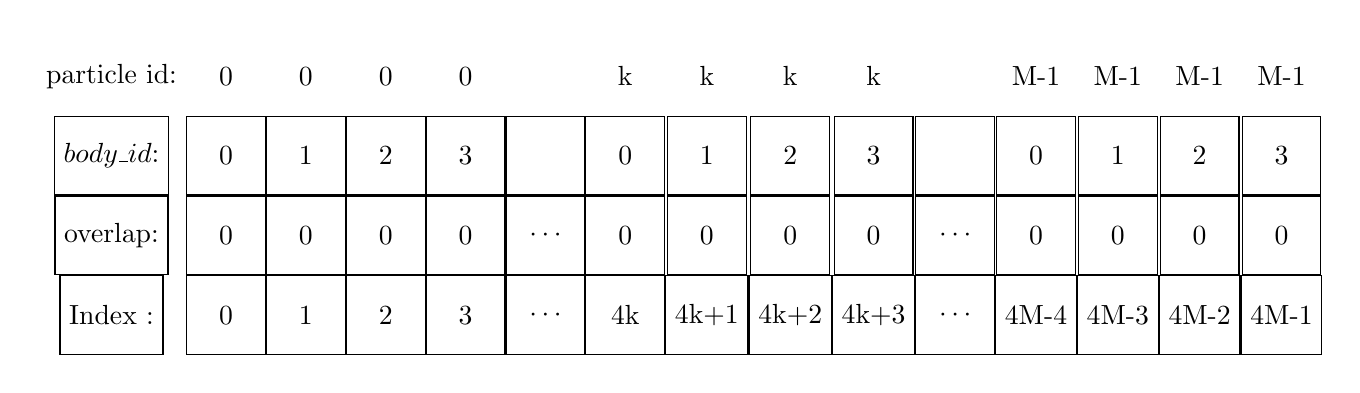
\begin{tikzpicture}
    \matrix (m) [matrix of nodes,
    nodes={draw, minimum size=10mm,anchor=center},
    nodes in empty cells, minimum height = 1cm,
    row 1/.style={nodes={draw=none}},]
    {
      particle id: & 0 & 0 & 0 & 0 &          & k  & k    & k    & k    &          & M-1  & M-1  & M-1  & M-1 \\
      $body\_id$:  & 0 & 1 & 2 & 3 &          & 0  & 1    & 2    & 3    &          & 0    & 1    & 2    & 3 \\
      overlap:     & 0 & 0 & 0 & 0 & $\cdots$ & 0  & 0    & 0    & 0    & $\cdots$ & 0    & 0    & 0    & 0\\
      Index  :     & 0 & 1 & 2 & 3 & $\cdots$ & 4k & 4k+1 & 4k+2 & 4k+3 & $\cdots$ & 4M-4 & 4M-3 & 4M-2 & 4M-1\\
    };
  \end{tikzpicture}
  \caption{An array to track the pairwise quantities. A stride of length $4$ is
    assigned to each particle to track the pairwise quantity.}
\label{fig:stride_index_trace}
\end{figure}

At an intermediate time $t_1$, let us assume that a particle with an index $k$ of body
$1$ is in contact with body $2$ and particle with index $l$ with body $3$ as seen in
\cref{fig:id:four_bodies_contact}. The updated overlap amount of particles $k$
and $l$ is given in \cref{fig:id:k_f_overlap_t_1},
\begin{figure}[!htpb]
  \centering
  \footnotesize
  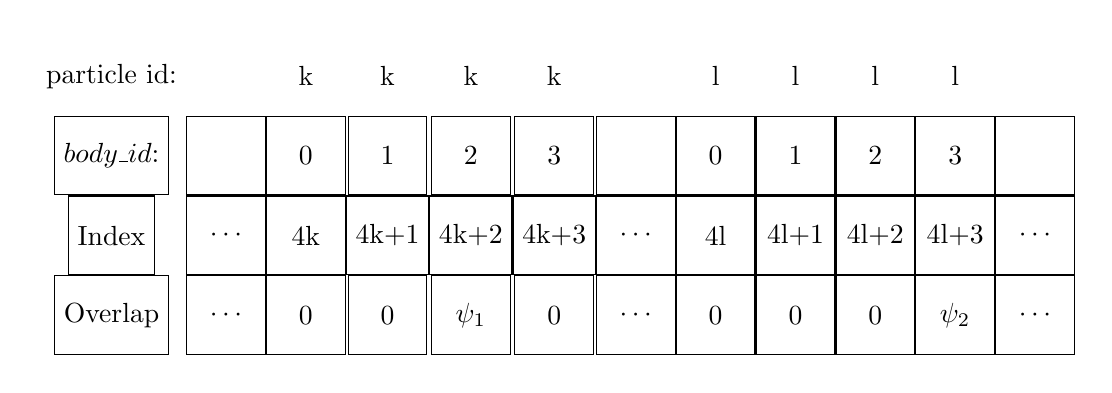
\begin{tikzpicture}
    \matrix (m) [matrix of nodes,
    nodes={draw, minimum size=10mm,anchor=center},
    nodes in empty cells, minimum height = 1cm,
    row 1/.style={nodes={draw=none}},]
    {
      particle id: & & k & k & k & k & & l & l & l & l &  \\
      $body\_id$:  & & 0 & 1 & 2 & 3 & & 0 & 1 & 2 & 3 &  \\
      Index & $\cdots$ & 4k & 4k+1 & 4k+2 & 4k+3 & $\cdots$ & 4l & 4l+1 & 4l+2 & 4l+3 & $\cdots$ \\
      Overlap & $\cdots$ & 0 & 0 & $\psi_1$ & 0 & $\cdots$ & 0 & 0 & 0 & $\psi_2$ & $\cdots$ \\
    };
  \end{tikzpicture}
  \caption{Updated overlap amount of particles $k$ and $l$.}
\label{fig:id:k_f_overlap_t_1}
\end{figure}
where $\psi$ in the figure is a real number. Since particle $k$ is in contact
with body id $2$, we can see from \cref{fig:id:k_f_overlap_t_1} that the overlap
amount of particle $k$ with body id $2$ is saved as $\psi_1$. This overlap
amount is saved at its fixed array index of $4k+2$. Since particle $l$ is in
contact with body id $3$, we save the overlap with body $3$ at $4l+3$ index.
Similarly, let us assume a particle with an index $q$ is in contact with the
body $2$ and $3$. The pairwise array belonging to the particle $q$ is shown in
\cref{fig:id:overlap_of_q_at_t_1}. From \cref{fig:id:overlap_of_q_at_t_1}, we
can see that the pairwise overlap quantity of particle $q$ with bodies $2$ and
$3$ are saved at the indices of $4q+2$ and $4q+3$, respectively.
\begin{figure}[!htpb]
  \centering
  \footnotesize
  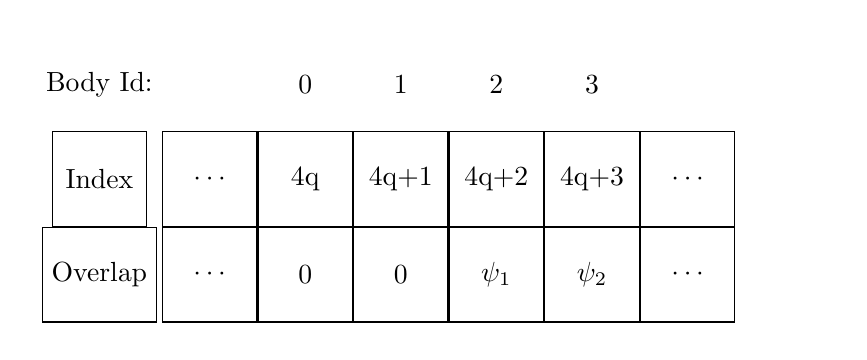
\begin{tikzpicture}
    \matrix (m) [matrix of nodes,
    nodes={draw, minimum size=12mm,anchor=center},
    nodes in empty cells, minimum height = 1cm,
    row 1/.style={nodes={draw=none}},]
    {
      Body Id: & & 0 & 1 & 2 & 3 & & \\
      Index & $\cdots$ & 4q & 4q+1 & 4q+2 & 4q+3 & $\cdots$ \\
      Overlap & $\cdots$ & 0 & 0 & $\psi_1$ & $\psi_2$ & $\cdots$ \\
    };
  \end{tikzpicture}
  \caption{Overlap amount of particle $q$ when in contact with bodies $2$ and $3$.}
  \label{fig:id:overlap_of_q_at_t_1}
\end{figure}

At the time ($t_3$), let the particle $l$ lose its collision with body $3$,
while particle $k$ is still in contact with body $2$. The updated overlap array
for this configuration is shown in \cref{fig:id:overlap_of_k_f_at_t_2}. From
\cref{fig:id:overlap_of_k_f_at_t_2}, we can see that we have updated the
pairwise tracking quantity, overlap, we make the overlap array value at index
$4l+3$ zero, as the particle $l$ lost contact with body $3$. However, we keep
the overlap value of particle $k$ with body $2$ since it didn't lose contact
with it.

\begin{figure}[!htpb]
  \centering
  \footnotesize
  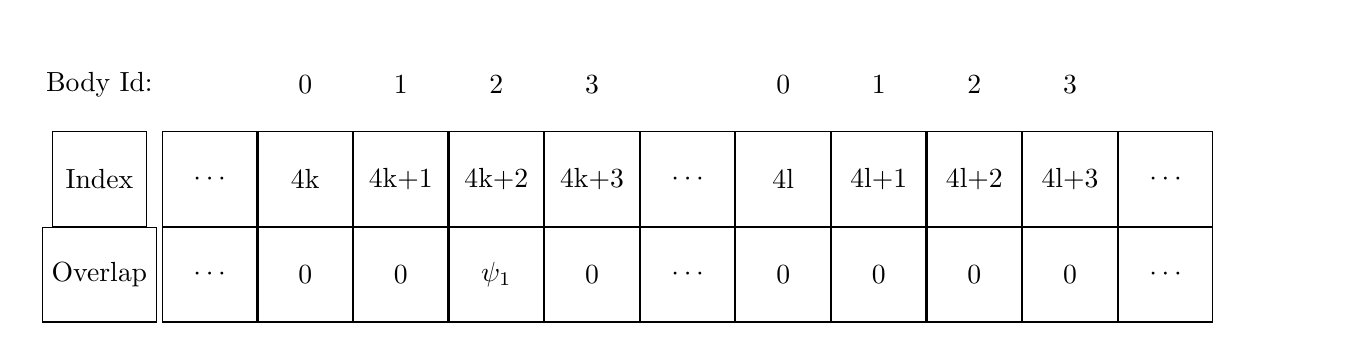
\begin{tikzpicture}
    \matrix (m) [matrix of nodes,
    nodes={draw, minimum size=12mm,anchor=center},
    nodes in empty cells, minimum height = 1cm,
    row 1/.style={nodes={draw=none}},]
    {
      Body Id: & & 0 & 1 & 2 & 3 & &  0 & 1 & 2 & 3 & & \\
      Index & $\cdots$ & 4k & 4k+1 & 4k+2 & 4k+3 & $\cdots$ & 4l & 4l+1 & 4l+2 & 4l+3 & $\cdots$ \\
      Overlap & $\cdots$ & 0 & 0 & $\psi_1$ & 0 & $\cdots$ & 0 & 0 & 0 & 0 & $\cdots$ \\
    };
  \end{tikzpicture}
  \caption{Overlap array of body $1$, showing the specific indices of
    particles $k$ and $l$ at time $t_2$.}
\label{fig:id:overlap_of_k_f_at_t_2}
\end{figure}
While letting particle $q$ lose its contact with bodies $2$ and $3$ and come
into contact with body $0$. In this case, the updated overlap array for the
indices belonging to the particle $q$ is given in
\cref{fig:id:overlap_of_q_at_t_2}. Similar to particle $k$ and $l$, we update
the pairwise tracking quantity, however, we save the overlap amount of particle
$q$ with body $0$ and make overlap amounts to zero for the indices of $4q+2$ and
$4q+3$.
\begin{figure}[!htpb]
  \centering
  \footnotesize
  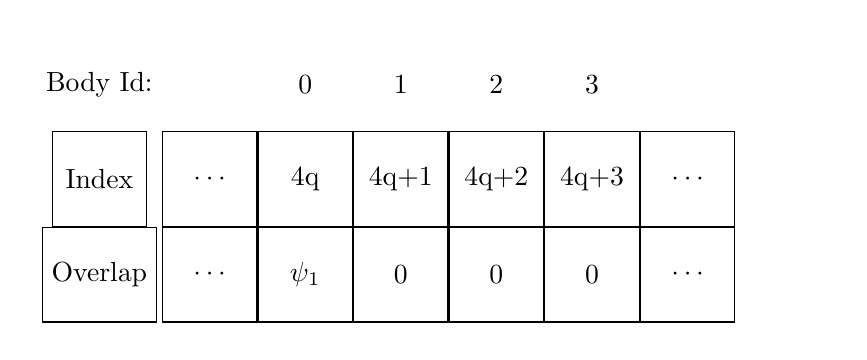
\begin{tikzpicture}
    \matrix (m) [matrix of nodes,
    nodes={draw, minimum size=12mm,anchor=center},
    nodes in empty cells, minimum height = 1cm,
    row 1/.style={nodes={draw=none}},]
    {
      Body Id: & & 0 & 1 & 2 & 3 & & \\
      Index & $\cdots$ & 4q & 4q+1 & 4q+2 & 4q+3 & $\cdots$ \\
      Overlap & $\cdots$ & $\psi_1$ & 0 & 0 & 0 & $\cdots$ \\
    };
  \end{tikzpicture}
  \caption{Overlap array of body $1$, showing the index of
    particle $q$ at time $t_2$.}
\label{fig:id:overlap_of_q_at_t_2}
\end{figure}
In the next section we look at the code to implement this algorithm in
PySPH.

\subsection{Implementation in PySPH}
We implement the above algorithm in PySPH using the following code. We first
create a particle array with the required properties. A sample code segment
describing the creation of a particle array is given as
\lstset{caption={Code segment for the creation of a particle array.}} \lstset{basicstyle=\footnotesize\ttfamily}
\begin{lstlisting}[label={contact:equations},frame=lines,language=Python,upquote=True]
body_2 = get_particle_array(x=[0., 1., 2., 3.],
                            y=[0., 0., 0., 0.],
                            # ... Code redacted ...
                            name="body")
\end{lstlisting}

To implement the pairwise tracking algorithm, we add an additional property with
a stride. In our case, a particle can contact four bodies at a given time. A
property of stride length $4$ is added to the particle array as
\lstset{caption={Code segment to add a stride property to an existing particle
    array.}} \lstset{basicstyle=\footnotesize\ttfamily}
\begin{lstlisting}[label={contact:equations},frame=lines,language=Python,upquote=True]
body_2.add_property(name='overlap', stride=4)
\end{lstlisting}
The pairwise interactions are computed with the following code
\lstset{caption={Code snippet to handle tracking of pairwise interactions with a few number of bodies.}} \lstset{basicstyle=\footnotesize\ttfamily}
\begin{lstlisting}[label={contact:equations},frame=lines,language=Python,upquote=True]
class ComputeContactForce(Equation):
    def initialize(self, d_idx, d_overlap, d_total_no_bodies, dt, t):
        i, t1, t2 = declare('int', 3)

        t1 = d_total_no_bodies[0] * d_idx

        for i in range(d_total_no_bodies[0]):
            t2 = t1 + i
            d_overlap[t2] = 0.

    def loop(self, d_idx, d_total_no_bodies, s_idx,
            s_body_id, dt, RIJ):
        t1, t2 = declare('int', 2)

        t1 = d_total_no_bodies[0] * d_idx
        t2 = t1 + s_body_id[s_idx]

        d_overlap[t2] += RIJ
        # ... Code redacted ...
\end{lstlisting}
Here, \texttt{d\_total\_no\_bodies} is the total number of bodies in a given
case. In the above code listing, in order to compute the overlap of the
particles on a given body with the other bodies, we first initialize the
pairwise quantity, overlap, to zero. \texttt{initialize} method depicts the
initialization of overlap to zero. In \texttt{loop} method, we compute the pairwise
overlap of the particle when colliding with the bodies. We compute the forces on
the bodies using the above equation using the \texttt{Group} function in PySPH
\texttt{Application} class routine as, 2.1 $2.1$
\lstset{caption={Code segment to compute the forces on the bodies.}} \lstset{basicstyle=\footnotesize\ttfamily}
\begin{lstlisting}[label={contact:equations},frame=lines,language=Python,upquote=True]
  Group(equations=[
      ComputeContactForce(dest='body_0', sources=[
          'body_1', 'body_2', 'body_3']),
      ComputeContactForce(dest='body_1', sources=[
          'body_1', 'body_2', 'body_3']),
      ComputeContactForce(dest='body_2', sources=[
          'body_1', 'body_2', 'body_3']),
      ComputeContactForce(dest='body_3', sources=[
          'body_0', 'body_1', 'body_2'])
    ])
\end{lstlisting}
We execute the equation of computation of the contact force of each body due to the
\texttt{sources}. Four equations are used to compute the forces on four bodies due to
the interaction with the other three bodies.


\section{Contact Force Modeling with a Large Number of Particles}
\label{sec:tracking-many-bodies}
In the previous section, we used a strided array with a fixed index per
interaction to handle the tracking of pairwise interactions while computing the
contact force on a particle due to the interaction with other bodies. However, a
fixed index per interaction is not favorable when dealing with simulations
involving a large number of bodies or particles. This is because, a very large
stride is wasteful in terms of memory. For cases with a large number of bodies,
we propose an algorithm where dynamic addition and removal of contacts are
involved. Further, this algorithm is feasible in cases when the particle at a
given time will not have more than a fixed number of contacts to track. In the
current section, we demonstrate the dynamic contact handling algorithm. We
consider two cases, one where all the particles belong to the same particle
array and another case where particles belonging to two different particle
arrays interact with each other and among themselves.

\subsection{Single Particle Array}
\begin{figure}[!htpb]
  \centering
  \includegraphics[width=0.3\textwidth]{images/implementation_detail/images/many_bodies/many_bodies_t_0}
  \caption{Particles with finite radius at time $t=0$.}
\label{fig:id:15_particle_t_0}
\end{figure}

To demonstrate the dynamic tracking algorithm, we consider the interaction of
$15$ particles as shown in \cref{fig:id:15_particle_t_0}. We assume, at a given
time, no particle can have more than $3$ contacts. We demonstrate the algorithm
when the particles are initiated in a single particle array, such that no two
particles have the same index. Since, with a large number of bodies involved, we
do not have a prefixed index for the pairwise interaction, we additionally need
to save the index of the contacting particle in addition to the pairwise contact
properties. \Cref{fig:many_bodies_initialize_overlap_t_0}, shows the additional
property, \texttt{contact\_id}, added to the particle array to track the indices which a
given particle of index $k$ is in contact with. The contact indices are
initialized to $-1$ and other pairwise interaction properties are initialized to
$0$ similar to the previous algorithm.
\begin{figure}[!htpb]
  \centering
  \footnotesize
  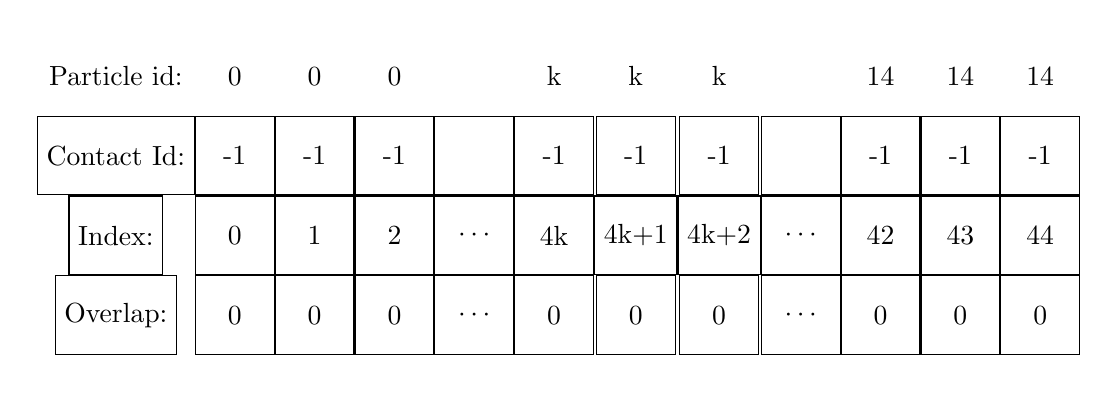
\begin{tikzpicture}
    \matrix (m) [matrix of nodes,
    nodes={draw, minimum size=10mm,anchor=center},
    nodes in empty cells, minimum height = 1cm,
    row 1/.style={nodes={draw=none}},]
    {
      Particle id: & 0 & 0 & 0 & & k & k & k & & 14 & 14  & 14 \\
      Contact Id: & -1 & -1 & -1 &  & -1 & -1 & -1 & & -1 & -1 & -1  \\
      Index: & 0 & 1 & 2 & $\cdots$ & 4k & 4k+1 & 4k+2 & $\cdots$ & 42 & 43 & 44 \\
      Overlap: & 0 & 0 & 0 & $\cdots$ & 0 & 0 & 0 & $\cdots$ & 0 & 0 & 0 \\
    };
  \end{tikzpicture}
  \caption{Values of strided array properties to handle the tracking of many bodies at time $t=0$.}
\label{fig:many_bodies_initialize_overlap_t_0}
\end{figure}

Code fragment of adding the new stride properties is given as
\lstset{caption={Code fragment to add the property required to track dynamics contacts.}} \lstset{basicstyle=\footnotesize\ttfamily}
\begin{lstlisting}[label={contact:equations},frame=lines,language=Python,upquote=True]
  pa.add_property('contact_id', stride=3, type="int")
  pa.contact_id[:] = -1
  pa.add_property(name='overlap', stride=3)
\end{lstlisting}

\begin{figure}[!htpb]
  \centering
  \includegraphics[width=0.3\textwidth]{images/implementation_detail/images/many_bodies/many_bodies_t_1}
  \caption{Configuration of particles at an intermediate time $t_1$.}
\label{fig:id:15_particle_t_1}
\end{figure}
%
The configuration of particles at an intermediate time $t_1$ are shown in
\cref{fig:id:15_particle_t_1}. Particles marked in red are contacts of $1$, $8$,
and $11$ particles. From \cref{fig:id:15_particle_t_1}, we can see that
particle with index $1$ is in contact with $0, 6, 7$ particles and a particle
with index $8$ with $5$ and $9$. Let us assume the contacts are formed for the
first time. \Cref{fig:many_bodies_initialize_overlap_1_8_11_t_1} shows the
updated overlap array of the contact indices, including the overlap for the
particles with index $1, 8$, and $11$.
\begin{figure}[!htpb]
  \centering
  \footnotesize
  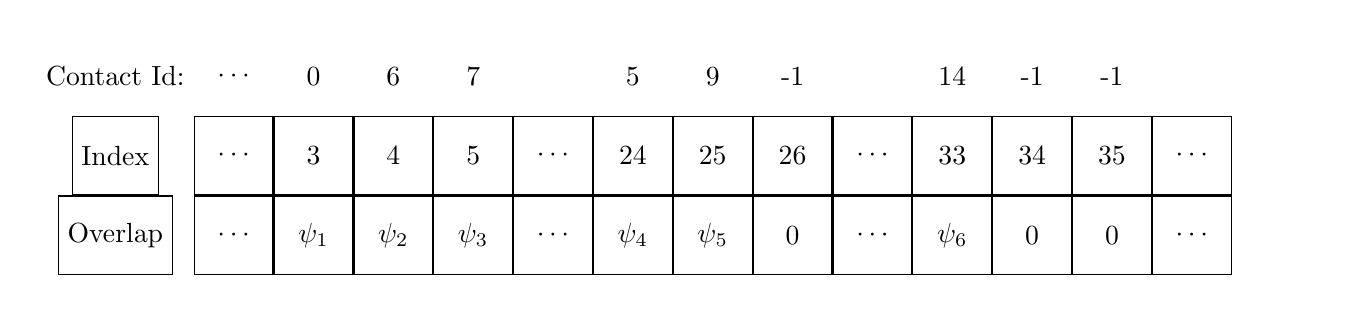
\begin{tikzpicture}
    \matrix (m) [matrix of nodes,
    nodes={draw, minimum size=10mm,anchor=center},
    nodes in empty cells, minimum height = 1cm,
    row 1/.style={nodes={draw=none}},]
    {
      Contact Id: & $\cdots$ & 0 & 6 & 7 &  & 5 & 9 & -1 & & 14 & -1 & -1 & & \\
      Index & $\cdots$ & 3 & 4 & 5 & $\cdots$ & 24 & 25 & 26 & $\cdots$ & 33 & 34 & 35 & $\cdots$\\
      Overlap  &$\cdots$ & $\psi_1$ & $\psi_2$ & $\psi_3$ & $\cdots$ & $\psi_4$ & $\psi_5$ & 0 & $\cdots$ & $\psi_6$ & 0 & 0 & $\cdots$ \\
    };
  \end{tikzpicture}
  \caption{Updated Contact Id and Overlap array at an intermediate time $t_1$.}
\label{fig:many_bodies_initialize_overlap_1_8_11_t_1}
\end{figure}

Dynamic pairwise contact tracking is handled in two parts. The first part is to
update the tracking array by removing the indices which are no more in contact.
As a second step, we add new contacts. We use two equations to implement it in
PySPH. One equation is used to add new contacts and update the values of the
existing contacts, while the second equation can be used to remove the
indices that are no more in contact. We outline the code to add new contacts and
update the existing ones in the following code snippet.
\lstset{caption={Code snippet to add new contact and update existing contact properties in dynamic
    pairwise tracking algorithm.}} \lstset{basicstyle=\footnotesize\ttfamily}
\begin{lstlisting}[label={code:add_contacts_many},frame=lines,language=Python,upquote=True]
class AddParticlesInContact(Equation):
    def loop(self, d_idx, d_m, d_contact_id, d_overlap, d_total_contacts,
             d_max_contacts_limit, RIJ, d_rad, s_idx, s_rad):
        p, q1, tot_ctcs, j, found_at, found = declare('int', 6)
        overlap = -1.

        # check the particles are not on top of each other.
        if RIJ > 1e-12:
            overlap = d_rad[d_idx] + s_rad[s_idx] - RIJ

        # ---------- force computation starts ------------
        # if particles are overlapping
        if overlap > 0:
            # total number of contacts of particle i in destination
            tot_ctcs = d_total_contacts[d_idx]

            # d_idx has a range of tracking indices with sources
            # starting index is p
            p = d_idx * d_max_contacts_limit[0]
            # ending index is q -1
            q1 = p + tot_ctcs

            # check if the particle is in the tracking list
            # if so, then save the location at found_at
            found = 0
            for j in range(p, q1):
                if s_idx == d_contact_id[j]:
                    found_at = j
                    found = 1
                    break
            # if the particle is not been tracked then assign an
            # index in tracking history.
            if found == 0:
                found_at = q1
                d_contact_id[found_at] = s_idx
                d_total_contacts[d_idx] += 1

            # implies we are tracking the particle
            else:
                # Save the pair wise quantity at found_at
                d_overlap[found_at] = overlap
\end{lstlisting}


\begin{figure}[!htpb]
  \centering
  \includegraphics[width=0.3\textwidth]{images/implementation_detail/images/many_bodies/many_bodies_t_2}
  \caption{configuration of particles at time $t_2$.}
\label{fig:id:15_particle_t_2}
\end{figure}

\Cref{fig:id:15_particle_t_2} shows the particles positions at time $t_2$. From
\cref{fig:id:15_particle_t_2}, we can see that a few particles lose contacts,
and a few gain new contacts. We will add the new particles to the tracking array
using the above code. However, after every time step, first we need to update
the tracking array by removing the indices that are no more in contact.
\Cref{fig:many_bodies_initialize_overlap_1_8_11_t_2} shows the updated contact
indices array and the overlapping array at time $t_2$.
\begin{figure}[!htpb]
  \centering
  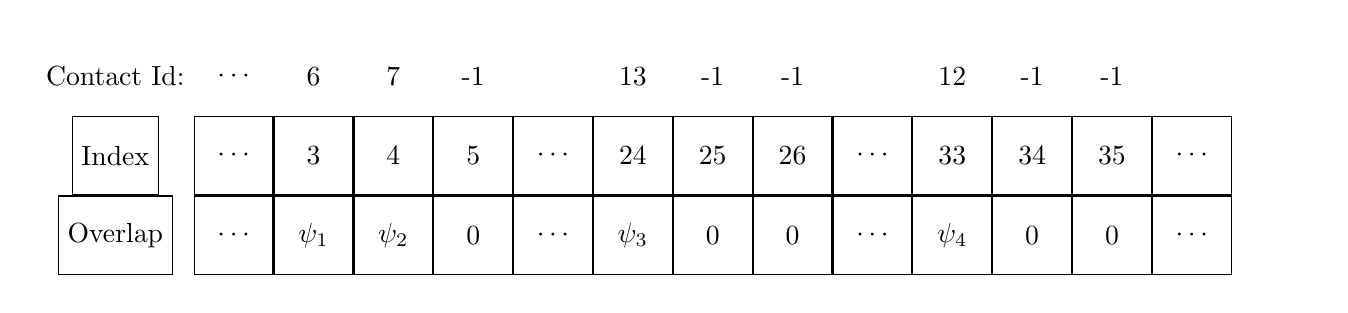
\begin{tikzpicture}
    \matrix (m) [matrix of nodes,
    nodes={draw, minimum size=10mm,anchor=center},
    nodes in empty cells, minimum height = 1cm,
    row 1/.style={nodes={draw=none}},]
    {
      Contact Id: & $\cdots$ & 6 & 7 & -1 &  & 13 & -1 & -1 & & 12 & -1 & -1 & & \\
      Index & $\cdots$ & 3 & 4 & 5 & $\cdots$ & 24 & 25 & 26 & $\cdots$ & 33 & 34 & 35 & $\cdots$\\
      Overlap  &$\cdots$ & $\psi_1$ & $\psi_2$ & 0 & $\cdots$ & $\psi_3$ & 0 & 0 & $\cdots$ & $\psi_4$ & 0 & 0 & $\cdots$ \\
    };
  \end{tikzpicture}
  \caption{Updated Contact Id and Overlap array at an intermediate time $t_2$}
\label{fig:many_bodies_initialize_overlap_1_8_11_t_2}
\end{figure}

The following code snippet is used to remove the contacts that are no more in
contact with the particle.
\lstset{caption={Code snippet to remove lost contacts in dynamic pairwise tracking algorithm.}} \lstset{basicstyle=\footnotesize\ttfamily}
\begin{lstlisting}[label={contact:equations},frame=lines,language=Python,upquote=True]
class RemoveParticlesNotInContact(Equation):
    def initialize_pair(self, d_idx, d_x, d_y, d_z, d_rad,
                        d_total_contacts, d_contact_id,
                        d_max_contacts_limit, d_overlap,
                        s_rad):
        # Declare variable: Code redacted

        idx_total_ctcs = d_total_contacts[d_idx]
        # particle idx contacts has range of indices
        # and the first index would be
        p = d_idx * d_max_contacts_limit[0]
        last_idx_tmp = p + idx_total_ctcs - 1
        k = p
        count = 0

        # loop over all the contacts of particle d_idx
        while count < idx_total_ctcs:
            # The index of the particle with which
            # d_idx in contact is
            sidx = d_contact_id[k]

            if sidx == -1:
                break
            else:
                xij[0] = d_x[d_idx] - s_x[sidx]
                xij[1] = d_y[d_idx] - s_y[sidx]
                xij[2] = d_z[d_idx] - s_z[sidx]
                rij = sqrt(xij[0] * xij[0] + xij[1] * xij[1] +
                           xij[2] * xij[2])

                overlap = d_rad_s[d_idx] + s_rad_s[sidx] - rij

                if overlap <= 0.:
                    # if the swap index is the current index then
                    # simply make it to null contact.
                    if k == last_idx_tmp:
                        d_contact_id[k] = -1
                        d_overlap[k] = 0.
                    else:
                        # swap the current tracking index with the final
                        # contact index
                        d_contact_id[k] = d_contact_id[last_idx_tmp]
                        d_contact_id[last_idx_tmp] = -1

                        # swap tangential x displacement
                        d_overlap[k] = d_overlap[last_idx_tmp]
                        d_overlap[last_idx_tmp] = 0.

                        # decrease the last_idx_tmp, since we swapped it to
                        # -1
                        last_idx_tmp -= 1

                    # decrement the total contacts of the particle
                    d_total_contacts[d_idx] -= 1
                else:
                    k = k + 1
                count += 1
\end{lstlisting}

The above equations are used in the \texttt{create\_equations} method of \texttt{Application}
class of PySPH to execute in execution loop using the following code.
\lstset{caption={An equation execution order to handle the pairwise tracking algorithm in PySPH.}} \lstset{basicstyle=\footnotesize\ttfamily}
\begin{lstlisting}[label={contact:equations},frame=lines,language=Python,upquote=True]
  Group(equations=[
      RemoveParticlesNotInContact(dest='grains',
      sources=['grains'])
    ]),
  Group(equations=[
      AddParticlesInContact(dest='grains', sources=['grains'])
    ]),
\end{lstlisting}


\subsection{Dealing with Multiple Particle Arrays}
Let us consider a case where particles of two different particle arrays
interact with each other. A schematic is shown in \cref{fig:mb:2_pa}. Here,
we consider each particle array to have $15$ particles, as shown in
\cref{fig:mb:2_pa}.
\begin{figure}[!htpb]
  \centering
  \includegraphics[width=0.7\textwidth]{images/implementation_detail/images/many_bodies/many_bodies_two_pa_t_0}
  \caption{}
\label{fig:mb:2_pa}
\end{figure}
Let's name particle array $1$ as \texttt{grains\_1} and particle array $2$ as
\texttt{grains\_2}. As described in the previous section, in PySPH, to compute
the interaction, we use the following code snippet.
\lstset{caption={Code snipped to compute contact force on particle arrays.}}
\lstset{basicstyle=\footnotesize\ttfamily}
\begin{lstlisting}[label={contact:equations},frame=lines,language=Python,upquote=True]
  Group(equations=[
      RemoveParticlesNotInContact(dest='grains_1',
          sources=['grains_1', 'grains_2'])
      RemoveParticlesNotInContact(dest='grains_2',
          sources=['grains_1', 'grains_2'])
    ]),
  Group(equations=[
      AddParticlesInContact(dest='grains_1',
          sources=['grains_1', 'grains_2'])
      AddParticlesInContact(dest='grains_2',
          sources=['grains_1', 'grains_2'])
    ]),
\end{lstlisting}


Let us consider the computation of contact force on particles belonging to
particle array 1. From the previous algorithm, we initialize the
\texttt{contact\_id} and \texttt{overlap} arrays to particle array $1$ as shown
in \cref{fig:mb-2-pa-prev-algo}.
\begin{figure}[!htpb]
  \centering
  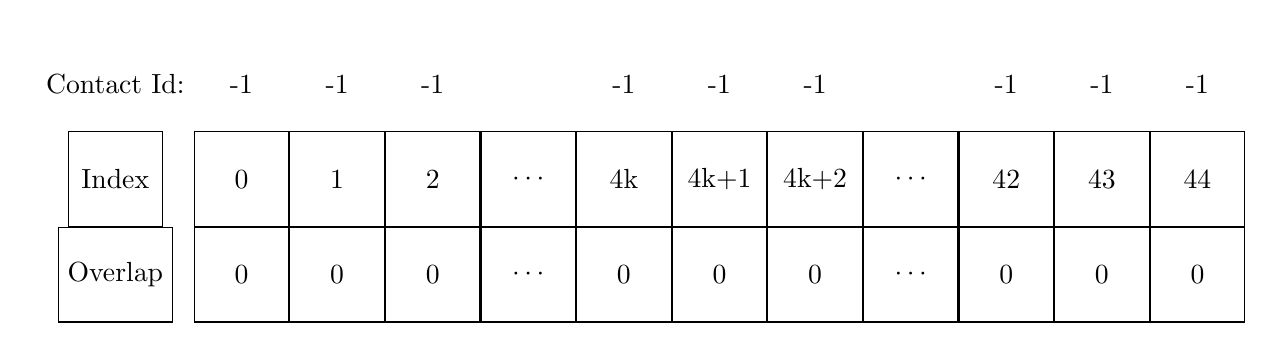
\begin{tikzpicture}
    \matrix (m) [matrix of nodes,
    nodes={draw, minimum size=12mm,anchor=center},
    nodes in empty cells, minimum height = 1cm,
    row 1/.style={nodes={draw=none}},]
    {
      Contact Id: & -1 & -1 & -1 &  & -1 & -1 & -1 & & -1 & -1 & -1  \\
      Index & 0 & 1 & 2 & $\cdots$ & 4k & 4k+1 & 4k+2 & $\cdots$ & 42 & 43 & 44 \\
      Overlap & 0 & 0 & 0 & $\cdots$ & 0 & 0 & 0 & $\cdots$ & 0 & 0 & 0 \\
    };
  \end{tikzpicture}
  \caption{Contact Id and Overlap array for particle array 1.}
\label{fig:mb-2-pa-prev-algo}
\end{figure}

\Cref{fig:mb-2-pa-t-2} shows the particle arrays' particles
interacting with each other. From \cref{fig:mb-2-pa-t-2}, we can see particles
of both arrays interact with each other. \Cref{fig:zoomed-8-id} depicts
contacts of particle with index $8$. The contact array and the pairwise overlap
of a particle with index $8$ are shown in \cref{fig:id-8-mb-array}. From
\cref{fig:id-8-mb-array,fig:zoomed-8-id}, we can see that the particle with
index $8$ is in contact with a particle of index $5$ of both the particle arrays
and with $1$ of particle array 2. The algorithm developed for a single particle
array fails to identify the contact properly, as there is no way to
differentiate between which particle array the given contacting particle belongs.
\begin{figure}[!htpb]
  \centering
  \includegraphics[width=0.5\textwidth]{images/implementation_detail/images/many_bodies/many_bodies_two_pa_t_1}
  \caption{Configuration of the particles at an intermediate time $t_1$.}
\label{fig:mb-2-pa-t-2}
\end{figure}
\begin{figure}[!htpb]
  \centering
  \includegraphics[width=0.2\textwidth]{images/implementation_detail/images/many_bodies/many_bodies_two_pa_t_1_zoomed}
  \caption{Contacts of particle with index $8$ with particles with index $5$
    both the particle arrays and index $1$.}
\label{fig:zoomed-8-id}
\end{figure}
\begin{figure}[!htpb]
  \centering
  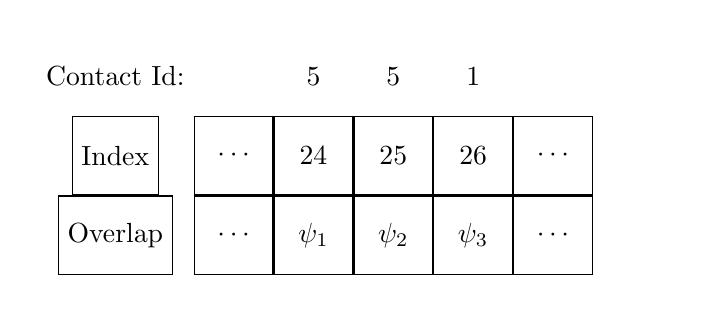
\begin{tikzpicture}
    \matrix (m) [matrix of nodes,
    nodes={draw, minimum size=10mm,anchor=center},
    nodes in empty cells, minimum height = 1cm,
    row 1/.style={nodes={draw=none}},]
    {
      Contact Id: & & 5 & 5 & 1 & & \\
      Index & $\cdots$ & 24 & 25 & 26 & $\cdots$\\
      Overlap  &$\cdots$ & $\psi_1$ & $\psi_2$ & $\psi_3$ & $\cdots$\\
    };
  \end{tikzpicture}
  \caption{Updated Contact Id and Overlap array at an intermediate time $t_1$,
    showing indices for particle $8$.}
\label{fig:id-8-mb-array}
\end{figure}

To solve this issue, we assign an additional property to the particles, a unique
id, to each different particle array. Such as, here, we would add a property
named \texttt{unique\_id}, where for each particle array, we would assign a
unique id. The updated tracking properties with the \texttt{unique\_id} included
is shown in \cref{fig:mb-ui-included}.
\begin{figure}[!htpb]
  \centering
  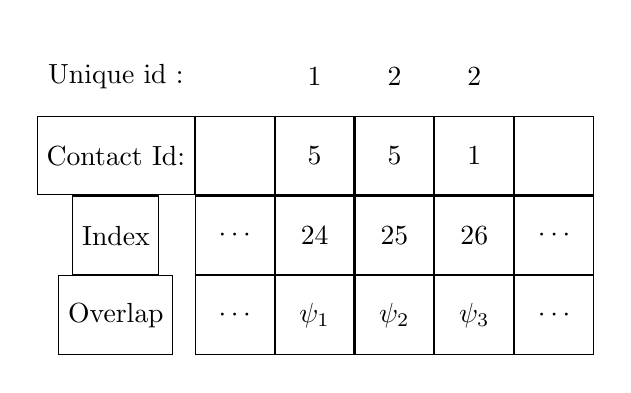
\begin{tikzpicture}
    \matrix (m) [matrix of nodes,
    nodes={draw, minimum size=10mm,anchor=center},
    nodes in empty cells, minimum height = 1cm,
    row 1/.style={nodes={draw=none}},]
    {
      Unique id : & & 1 & 2 & 2 & \\
      Contact Id: & & 5 & 5 & 1 & \\
      Index & $\cdots$ & 24 & 25 & 26 & $\cdots$\\
      Overlap  &$\cdots$ & $\psi_1$ & $\psi_2$ & $\psi_3$ & $\cdots$\\
    };
  \end{tikzpicture}
  \caption{Updated tracking properties of particle $8$ with unique id included.}
\label{fig:mb-ui-included}
\end{figure}
The updated code, with multiple particle arrays reads,
\lstset{caption={Code snippet to add new contact and update existing contact properties in
dynamic pairwise tracking algorithm with multiple particle arrays.}} \lstset{basicstyle=\footnotesize\ttfamily}
\begin{lstlisting}[label={contact:equations},frame=lines,language=Python,upquote=True]
class TrackTheOverlap(Equation):
    def loop(self, d_idx, d_m, d_contact_id, d_overlap, d_total_contacts,
            d_max_contacts_limit, RIJ, d_rad, s_idx, s_rad
            s_unique_id, d_contact_unique_idx):
        p, q1, tot_ctcs, j, found_at, found = declare('int', 6)
        overlap = -1.

        # check the particles are not on top of each other.
        if RIJ > 1e-12:
            overlap = d_rad[d_idx] + s_rad[s_idx] - RIJ

        # ---------- force computation starts ------------
        # if particles are overlapping
        if overlap > 0:
            # total number of contacts of particle i in destination
            tot_ctcs = d_total_contacts[d_idx]

            # d_idx has a range of tracking indices with sources
            # starting index is p
            p = d_idx * d_max_contacts_limit[0]
            # ending index is q -1
            q1 = p + tot_ctcs

            # check if the particle is in the tracking list
            # if so, then save the location at found_at
            found = 0
            for j in range(p, q1):
                if s_idx == d_contact_id[j] and \
                   s_unique_id[s_idx] == d_contact_unique_idx[j]:
                    found_at = j
                    found = 1
                    break
            # if the particle is not been tracked then assign
            # an index in tracking history.
            if found == 0:
                found_at = q1
                d_contact_id[found_at] = s_idx
                d_contact_unique_idx[found_at] = s_unique_id[s_idx]
                d_total_contacts[d_idx] += 1

            # implies we are tracking the particle
            else:
                # Save the pair wise quantity at found_at
                d_overlap[found_at] = overlap
\end{lstlisting}
In the above code, we have additionally added a check to the existing single
particle array code. This check ensures that the indices we are tracking belong
to the correct particle array.


\subsection{Sand in a Rotating Drum}
\label{sec:dem-drum-case}
This example demonstrates the implementation in simulating motion of sand in a
rotating drum. The algorithms discussed in \cref{sec:tracking-many-bodies} are
used to handle the contact between the sand particles. The dynamics of the
particles follow the formulation by \textcite{cundall_discrete_1979} and
\textcite{luding_dem_2008}. The drum is initially static and starts rotating with an
angular velocity of 5 rad/s after the sand settles down. Figure 14 shows the
arrangement of the sand particles, the top row depicts the results when the drum
is not rotating, while the bottom row is when the drum is rotating. This shows
that PySPH provides the features required to implement a variety of different
meshless methods.
\begin{figure}
  \centering
  \includegraphics[width=0.6\textwidth]{images/implementation_detail/images/many_bodies/dem_rolling_drum_case}
  \caption{Positions of the sand in a drum, color indicates the velocity magnitude. The top row depicts the
results when the drum is not rotating, and the bottom row is when the drum is rotating.}
\label{fig:dem_drum}
\end{figure}


\section{Sub-stepping Update Algorithm}
\label{sec:substepping-algorithm}
Problems involving two different materials, such as fluid-structure interaction,
rigid-fluid coupling, etc., involve solving two different materials, such that
one material is stiffer than the other. Let us consider a problem that has both
fluid and solid particles. Assume timesteps of fluid and solid are related as
follows,
\begin{equation}
\Delta t_f = K \Delta t_s,
\end{equation}
where $K$ is some integer. We use a sub-stepping integration scheme to update
the state of \texttt{fluid} and \texttt{solid} particles. Let us say
\texttt{fluid} has $10,000$ particles, and the solid has $1000$ particles, and
let $K$ be $10$. Using a sub-stepping scheme, instead of iterating $10,000$
particles $10$ times, we only do it one time. We first move the higher timestep
material to the next timestep, here fluid, then update the material with lower
timestep $K$ times, such that the simulation is stable.
\begin{figure}[!htpb]
  \centering
  \includegraphics[width=1.0\textwidth]{images/implementation_detail/images/multiphase/time_stepping}
  \caption{Pictorial representation of the sub-stepping algorithm.}
\label{fig:id:multiphase}
\end{figure}
\Cref{fig:id:multiphase} depicts idea of sub-stepping algorithm. Here,
$\Delta t_{\text{factor}}$ is chosen as a timestep for \texttt{solid} particles.
$\Delta t_{\text{factor}}$ is computed based on two factors. One is it is a
integer multiple of $\Delta t_{\text{material 1}}$
(\cref{eqn:id:dt_factor_chose}) and the second is it has to be less than or
equal to $\Delta t_{\text{material 2}}$, such that the simulation is stable.
\begin{equation}
\label{eqn:id:dt_factor_chose}
\Delta t_{\text{factor}} = \frac{\Delta t_{\text{material 1}}}{K}
\end{equation}


\subsection{Implementation in PySPH}
\label{sec:pysph-substepping-algorithm}
The following integrator routine is used for the sub-stepping algorithm
\lstset{caption={Code snippet for integrator used in substepping.}}
\lstset{basicstyle=\footnotesize\ttfamily}
\begin{lstlisting}[label={contact:equations},frame=lines,language=Python,upquote=True]
class SubSteppingIntegrator(Integrator):
    def one_timestep(self, t, dt):
        self.compute_accelerations()
\end{lstlisting}
We can see that only one method \texttt{self.compute\_accelerations()} is
called at every timestep in a sub-stepping scheme. We use the PySPH feature of
being able to iterate a group of equations to implement this algorithm. We
iterate using the larger $\Delta t$ value, but inside that, we use an iterated
loop with the smaller timestep. The code listing of updating the particle
arrays with different timesteps is given as,
\lstset{caption={Code snippet for substepping algorithm in PySPH.}}
\lstset{basicstyle=\footnotesize\ttfamily}
\begin{lstlisting}[label={contact:equations},frame=lines,language=Python,upquote=True]
  Group(equations=[
      FluidEquations(dest='fluid', sources=['fluid', 'solid'],
                     dt=dt_1)
  ]),
  Group(equations=[
      Group(equations=[
          SolidEquations(dest='solid', sources=['fluid', 'solid'],
                         dt=dt_1/10)
      ])
  ]
  iterate=True, max_iterations=10, min_iterations=10)
\end{lstlisting}
Since here, \texttt{fluid} has a higher timestep, we first update it to the next
timestep using \texttt{FluidEquations} and the \texttt{solid} state is updated
to $t + \Delta t_1$ timestep using $10$ updates with a timestep of
$\frac{\Delta t_1}{10}$. At each iteration we advance the \texttt{solid} particles by
$\Delta t_1 / 10$ time using \texttt{SolidEquations} equations.


\section{Summary}
\label{sec:id:summary}
In the current chapter, we demonstrated the implementation details of the
algorithms developed in \cref{chap:ctvf,chap:csph}. The PySPH documentation has
implementation details of several algorithms implemented in the above chapters.
We discussed algorithms corresponding to the contact force interaction and
simulation involving two different materials with different timestep values.

A strided array approach is used to track the pairwise contacts. A fixed index
is assigned to the particle for each pairwise interaction with a few bodies
handled. In cases with many bodies, a similar strided approach is used. However,
the contacts are updated dynamically as the particles make and leave contacts.
\Cref{sec:contact-algorithm} utilizes the algorithm of contact tracking for
fewer bodies, while \cref{sec:dem-drum-case} follows the contact tracking
algorithm for many bodies.

A sub-stepping algorithm is discussed in which the material with a higher
timestep is updated first, then the stiffer phase is updated with a lower time
step but in $K$ intervals. We discussed the tools provided by PySPH in order to
implement the sub-stepping algorithm.

In the next chapter, we model the interaction between the fluid and the elastic
structure, fluid-structure interaction. We propose an updated Lagrangian model
by coupling the solver developed in \cref{chap:ctvf} to handle the
fluid-structure interaction problems.

\chapter{Fluid-Structure Interaction}\label{chap:fsi}
\section{Introduction}
In the current chapter, we use the CTVF scheme developed in \cref{chap:ctvf}
to model fluid-structure interaction problems. Fluid-structure interaction (FSI)
is a common engineering problem that is seen in daily life. Some examples
include the deformation of wind turbine blade due to the fluid flow, blood flow
in heart value, coastal engineering, and vortex-induced vibration
\parencite{williamson2004vortex,bearman2011circular}. An accurate study of FSI can
allow us to optimize the systems where FSI is dominant. However, studying the
FSI phenomena through experiments or analytical techniques are complex due to
their nonlinear behavior.

Handling FSI problems with the transport velocity formulation framework is
advantageous as it can solve the tensile instability issue in solid dynamics and
ensure a homogeneous particle distribution in fluids. In the current chapter, we handle
FSI problems by the CTVF method, where both fluids and solid phases are modeled
using CTVF alone. To validate the proposed method, we consider three numerical
test cases. A uniformly distributed load over a clamped beam (UDL) problem is
considered to validate the elastic dynamics of CTVF. An aluminum plate over a
hydrostatic tank for FSI validation is considered. Finally, it is applied to a
fluid flow striking an elastic plate. Here, the deformation of the elastic plate
is compared against the experimental results.

\section{Numerical Modeling}\label{sec2}
We follow the CTVF formulation to model both fluid and solid phases. The
particles are moved with a transport velocity rather than the momentum velocity,
which provides us with a homogenized particle distribution and eliminates
tensile instability. In the following two sections we briefly describe the
governing equations of the fluid and solid dynamics in discretized form.


\subsection{Discrete Equations of the Fluid and Solid Medium}\label{subsec:discrete-fluid}
The governing equations of the fluid are conservation of mass and momentum. We
follow the SPH discretization of the continuity
equation~\eqref{eq:fsi:sph-discretization-continuity} and the EDAC
based~\parencite{PRKP:edac-sph-iccm2015} pressure evolution
equation~\eqref{eq:fsi:sph-discretization-edac} given in \cref{chap:ctvf}, given
as
\begin{equation}
  \label{eq:fsi:sph-discretization-continuity}
  \frac{\tilde{d}\rho_a}{dt} = \sum_{b} \; \frac{m_b}{\rho_{b}} \; (
  \rho_{a} \; \tilde{\ten{u}}_{ab} \; + \;
  (\rho \; (\tilde{\ten{u}} \; - \;
  \ten{u}))_{ab}) \; \cdot \nabla_{a} W_{ab},
\end{equation}
\begin{multline}
  \label{eq:fsi:sph-discretization-edac}
  \frac{\tilde{d}p_a}{dt} = \sum_{b} \; \frac{m_b}{\rho_{b}} \; \bigg(
  (p_{a} - \rho_{a} c_{s}^2) \; \ten{u}_{ab} \; + \;
  p_{a} \; \tilde{\ten{u}}_{ab} \; - \;
  (p \; (\tilde{\ten{u}} - \ten{u}))_{ab} \; + \;\\
  4 \; \nu_{edac}
  \frac{p_a - p_b}{(\rho_a + \rho_b) (r^2_{ab} + 0.01 h_{ab}^{2})} \ten{r}_{ab}
  \bigg) \; \cdot \nabla_{a} W_{ab}.
\end{multline}
%
Here, the summation also includes the solid particles in the influence of a
fluid particle. The momentum equation is modified to consider the force
acting on the fluid particle due to the interaction with the elastic structure
particles. The discretized momentum equation is written as,
\begin{multline}
  \label{eq:fsi:sph-momentum-fluid}
  \frac{\tilde{d}\ten{u}_{a}}{dt} = - \sum_{b} m_b \bigg[
  \bigg(\frac{p_a}{\rho_a^2} + \frac{p_b}{\rho_b^2}\bigg) \ten{I} -
  \bigg(\frac{\ten{A}_a}{\rho_a^2} + \frac{\ten{A}_b}{\rho_b^2} + \Pi_{ab}
  \ten{I} \bigg) \bigg]
  \cdot \nabla_{a} W_{ab} \\
  + \ten{u}_{a} \sum_{b} \frac{m_b}{\rho_{b}} \; \tilde{\ten{u}}_{ab} \cdot
  \nabla_{a} W_{ab} \\+ \sum_{b} m_b \frac{4 \eta \nabla W_{ab}\cdot
    \ten{r}_{ab}}{(\rho_a + \rho_b) (r_{ab}^2 + 0.01 h_{ab}^2)} \ten{u}_{ab} +
  \ten{g}_{a} + \frac{\ten{F}^a_{\text{FSI}}}{m_a}
\end{multline}
$\ten{F}^a_{\text{FSI}}$ is the force due to the interaction with elastic
structure. This force modeling is explained in \cref{subsec:fsi}. We utilize the
ghost particle approach proposed in \parencite{Adami2012} to handle the boundaries.


Similar to the governing equations for the fluid, the governing equations of
the solid phase follow \cref{chap:ctvf} with a modification to the momentum
equation. We additionally need to consider the force due to the
fluid particles. The resulting equation is given as
\begin{multline}
  \label{eq:fsi:sph-momentum-solid}
  \frac{\tilde{d}\ten{u}_{a}}{dt} = - \sum_{b} m_b \bigg[
  \bigg(\frac{p_a}{\rho_a^2} + \frac{p_b}{\rho_b^2}\bigg) \ten{I} -
  \bigg(\frac{\teng{\sigma}^{'}_{a}}{\rho_a^2} +
  \frac{\teng{\sigma}^{'}_{b}}{\rho_b^2} + \Pi_{ab} \ten{I} \bigg) \bigg]  \cdot \nabla_{a} W_{ab}
  + \ten{g}_{a} + \frac{\ten{F}^a_{\text{FSI}}}{m_a}.
\end{multline}

We utilize SPST formulation described in \cref{sec:sunpst} to compute the
transport velocity of the fluid particles, while for the elastic phase
IPST \parencite{huang_kernel_2019} formulation is used.

\subsection{Fluid-Structure Interaction}\label{subsec:fsi}
Coupling is handled in a straight forward way in SPH. While modelling the fluid
phase and treating the fluid-structure interactions, the solid particles are
assumed to be boundary particles. From the boundary handling given in Adami
\parencite{Adami2012}, we compute the pressure of the boundary particles from
the extrapolated equation as,
\begin{equation}
  \label{eq:fsi:pressure-bc}
  p_s = \frac{\Sigma_f p_f W_{sf} + (\ten{g} - \ten{a}_{\ten{s}}) \cdot \Sigma_f
    \rho_f \ten{r}_{sf} W_{sf}}{\Sigma_f W_{sf}}.
\end{equation}
Here, $\ten{a}_s$ is the acceleration of the structure particles. The subscript
$f$ denotes the fluid particles and $s$ denotes the solid particles. Using the
extrapolated pressure, the hydrodynamic density of solid particles are
computed. Please note that the pressure we set here only pertain to the
FSI force and does not correspond to the real pressure or density of the
solid particles. By utilizing the previously set hydrodynamic properties on
the structure, the interaction force is computed using,
\begin{equation}
  \ten{F}_{\text{FSI}}^f = -m_f \sum_{s} m_s \bigg(\frac{p_f}{\rho_{f}^2} +
  \frac{p_s}{\rho_{s}^2} + \Pi_{fs} \bigg) \nabla_{f} W(x_{fs}).
\end{equation}


\section{Results And Discussion}\label{sec3}
In the current section we simulate three numerical examples to validate the
developed model. Deformation of a UDL plate due to external force and
hydrodynamics loads from a hydrostatic tank. Further, the model is applied to
study the deformation of an elastic obstacle due to the impact of fluid. A
convergence study is undertaken for both the UDL and elastic deformation under
hydrodynamic load problems. All the results are fully automated with the automan
package \parencite{automan2018} and made easy to reproduce. The source code for all
the problems demonstrated in this manuscript is made available at
\url{https://github.com/dineshadepu/fsi_etvf}.

% =========================================
% =========================================
% start
% =========================================
% =========================================
\subsection{Uniformly Distributed Loading (UDL) on a Clamped Beam}
\label{sec:udl}
In the first test case, we validate the structural part of the current solver.
We consider a homogeneous elastic plate clamped on both ends acted upon by a
uniformly distributed load ($q = 20$ Nm$\textsuperscript{-1}$) as shown in
\cref{fig:udl-schematic}. The beam's length (L) and height (H) is 0.2 m and
\begin{figure}
  \centering
  \includegraphics[scale=0.5]{images/fsi/images/khayyer_2021_udl/schematic}
  \caption{The schematic of a clamped elastic beam being acted upon by a
    uniformly distributed load.}
\label{fig:udl-schematic}
\end{figure}
$0.012$ m, respectively. The mechanical properties of the plate are set as
$E=10^7$ Pa in Young's modulus, $\nu=0$ in Poisson's ratio and $\rho=1000$
kgm$\textsuperscript{-3}$ in density. The numerical solution of the
y-displacement at the center of the beam is compared against the analytical
counterpart. The analytical solution for the deflection of a uniformly
distributed beam clamped at both ends is given by
\begin{equation}
  \label{eq:fsi:ce-tvf}
  \eta\left(\frac{L}{2}\right) = \frac{qL^4}{384 D},
\end{equation}
where, $D$ is defined as $\frac{E h^3}{12 (1 - (\nu)^2)}$. We consider three
particle resolutions such that, $10$, $15$, and $20$ particles along the beam's
width are used. We run for a total physical time of $2$ seconds.

\Cref{fig:udl-disp-plot} depicts the time history of y-displacement of the beam
center for different particle resolutions computed using the current solver
compared against the analytical solution. From \cref{fig:udl-disp-plot}, we can
see that the current solver can accurately predict the displacement of the
\begin{figure}
  \centering
  \includegraphics[scale=0.5]{figures/fsi/figures/khayyer_2021_udl/homogenous}
  \caption{Time variation of the y-displacement of the center of the beam for
    three different resolutions, compared against the analytical result.}
\label{fig:udl-disp-plot}
\end{figure}
clamped beam. Convergence of the current scheme is captured in
\cref{fig:udl-disp-plot}, and the computational results are within a reasonable
variation of the analytical solution with the variation of the particle spacing.


\subsection{Hydrostatic Water Column on an Elastic Plate}
\label{sec:hydrostatic-water-column-on-an-composite-elastic-plate}
In this example, we study the deformation of an elastic plate due to the
hydrostatic water column. We utilize the current example to examine the accuracy
and convergence of the current solver. The schematic of fluid with the elastic
beam is shown in \cref{fig:hs-water-on-plate} along with the initial pressure
distribution in the fluid. The figure includes the dimensions as well. The
material properties of the beam are, a density of $2700$
kgm\textsuperscript{-3}, with an Young's modulus of $67.5$ GPa, and a Poisson
\begin{figure}
  \centering
  \includegraphics[scale=0.4]{images/fsi/images/ng_2020_hydrostatic_water_column_on_elastic_plate/schematic}
  \caption{Schematic of the hydrostatic water column on an elastic plate. Fluid
    particle color represents pressure.}
\label{fig:hs-water-on-plate}
\end{figure}
ratio of $0.34$. The material properties of the fluid are, a density of $1000$
kgm\textsuperscript{-3}, with a zero dynamic viscosity. We consider three particle
resolutions such that we get $10$, $15$ and $20$ particles along the width
direction of the beam. We run the simulation for a total physical time of $3$
seconds. The y-displacement of the current solver at the center of the beam is
compared against the analytical result. The beam deflection computed using
an analytical expression results in a deflection $d = -6.85 \times 10^{-5}$ m.

\Cref{fig:snapshot-hs-fsi} shows the particle plot of the fluid along with the
elastic solid at time $2$ seconds with color of the fluid particles describing
the pressure. This snapshot corresponds to the highest particle resolution i.e.,
$20$ particles along the width direction. From the \cref{fig:snapshot-hs-fsi},
we can see that the current solver produces a smooth pressure distribution
\begin{figure}[!htpb]
  \centering
  \begin{subfigure}{0.48\textwidth}
    \centering
    \includegraphics[scale=1.0]{figures/fsi/figures/ng_2020_hydrostatic_water_column_on_elastic_plate/snap_t_0}
  \end{subfigure}
  \begin{subfigure}{0.48\textwidth}
    \centering
    \includegraphics[scale=1.0]{figures/fsi/figures/ng_2020_hydrostatic_water_column_on_elastic_plate/colorbar_t_0}
  \end{subfigure}
  \caption{ Snapshot of the fluid and the elastic structure at time 0.5 sec
   including the pressure of the fluid.}
\label{fig:snapshot-hs-fsi}
\end{figure}
demonstrating the stability of the current solver.
\Cref{fig:ng2020hsplate:deflection} depicts the time history of y-displacement
of the beam center for different particle resolutions computed using the current
solver compared against the analytical solution. From
\cref{fig:ng2020hsplate:deflection} we can see that the current solver is able
to predict the displacement of the clamped beam within the vicinity of the
analytical results. The current solver's beam displacement is closer to the
numerical results provided by \textcite{ng2020coupled}. The convergence of the
beam displacement is shown with the particle spacing is reduced.
\begin{figure}
  \centering
  \includegraphics[scale=0.5]{{{figures/fsi/figures/ng_2020_hydrostatic_water_column_on_elastic_plate/y_amplitude}}}
  \caption{The mid-span deflection of the structure under hydrodynamic loading
    with time for different resolutions, compared against the analytical and
    the numerical result of \parencite{ng2020coupled}.}
\label{fig:ng2020hsplate:deflection}
\end{figure}
%


\subsection{Water Impact onto an Elastic Plate}
\label{sec:water-impact-forefront}
In this case, we study the deformation of the elastic
plate due to the impact of water from a dam break.
\Cref{fig:dam-break-flow-impact-plate-initial-setup} shows the initial positions
of fluid and the structure inside the dam, including the dimensions. Following
\textcite{sun2019fully}, we set the material properties of the elastic plate with a
density of $2500$ kgm\textsuperscript{-3}, Young's modulus of $10^6$ Pa, and a
Poisson ratio of $0$. The material properties of the fluid are a density of 1000
kgm\textsuperscript{-3}, with no dynamic viscosity. A particle spacing of $5$
$\times$ $10^{-4}$ m is taken, resulting in a total of $182911$ particles, which
includes fluid, structure, and solid wall. We simulate a total physical time of
$0.7$ seconds. Here, the fluid is allowed to settle under gravity inside the
tank and attains a velocity as it reaches the elastic structure. The structure
will obstruct the fluid, making it rise, and the fluid will deform the elastic
plate. The rising fluid will hit the other end of the dam, come back, and hit
the structure from the back. We compare the current solver results to the other
numerical techniques for quantitative validation.
\begin{figure}
  \centering
  \includegraphics[scale=0.4]{images/fsi/images/sun_2019_dam_breaking_flow_impacting_an_elastic_plate/schematic}
  \caption{Schematic of the dam-break flow impacting an elastic plate. All dimensions are in meters.}
\label{fig:dam-break-flow-impact-plate-initial-setup}
\end{figure}

\begin{figure}
  \centering
  \includegraphics[scale=0.45]{figures/fsi/figures/sun_2019_dam_breaking_flow_impacting_an_elastic_plate/x_amplitude}
  \caption{Time histories of horizontal displacement of the free end of the
    elastic structure compared against the numerical results of
    \parencite{sun2019fully,bogaers2016evaluation}- Water impact onto an elastic
    plate.}
\label{fig:water-impact-plate-deflection-quantitative}
\end{figure}
\begin{figure}[H]
    \centering
  \begin{subfigure}{0.48\textwidth}
    \centering
        \includegraphics[scale=0.5]{figures/fsi/figures/sun_2019_dam_breaking_flow_impacting_an_elastic_plate/snap_t_0.png}
  \end{subfigure}

  \begin{subfigure}{0.48\textwidth}
    \centering
        \includegraphics[scale=0.5]{figures/fsi/figures/sun_2019_dam_breaking_flow_impacting_an_elastic_plate/snap_t_1.png}
  \end{subfigure}

  \begin{subfigure}{0.48\textwidth}
    \centering
        \includegraphics[scale=0.5]{figures/fsi/figures/sun_2019_dam_breaking_flow_impacting_an_elastic_plate/snap_t_2.png}
  \end{subfigure}

  \begin{subfigure}{0.48\textwidth}
    \centering
        \includegraphics[scale=0.5]{figures/fsi/figures/sun_2019_dam_breaking_flow_impacting_an_elastic_plate/snap_t_3.png}
  \end{subfigure}

  \begin{subfigure}{0.48\textwidth}
    \centering
    \includegraphics[scale=0.5]{figures/fsi/figures/sun_2019_dam_breaking_flow_impacting_an_elastic_plate/snap_t_4.png}
  \end{subfigure}
    \caption
    { Snapshot of the fluid and the structure at different time stamps. The
      color of the fluid particles represent the velocity magnitude. }
    \label{fig:dam-breaking-onto-plate-snapshot}
\end{figure}
The time variation of the x-displacement of the elastic structure is compared
against other numerical results~\parencite{sun2019fully,bogaers2016evaluation}.
From the \cref{fig:water-impact-plate-deflection-quantitative}, we can see that
the displacement computed by the current solver is within the vicinity of the
other results produced. The differences between the current solver with the
other numerical results are due to the linear stress-strain model used in the
current work. \Cref{fig:dam-breaking-onto-plate-snapshot} shows the snapshots of
the fluid and the elastic structure at different time instances. From
\cref{fig:dam-breaking-onto-plate-snapshot}, we can see that the fluid, after
hitting the structure, rises and hits the other end of the tank and travels back
to hit the structure again.

% ========================================================
% ========================================================
\section{Summary}\label{fsi:summary}
% ========================================================
% ========================================================
In the current chapter, we have handled the fluid-structure interaction using
the CTVF scheme developed in \cref{chap:ctvf}. Through particle shifting
techniques and incorporating the missing terms, we are able to eliminate several
issues SPH faces while solving fluid and solid problems. CTVF improves the
accuracy of fluid problems, and eliminates tensile instability while solving
elastic dynamics problems without any additional artificial stress terms.

We validated the developed scheme by solving a uniformly distributed load over a
clamped beam problem to test the structure equations, and an aluminum plate over
a hydrostatic tank where an analytical solution is available is utilized to
validate the FSI part of the current solver. The current solver is applied to a
dam break striking an elastic plate. Here, the deformation of the elastic plate
is compared to the computational results of other numerical models. A
convergence analysis is undertaken for both fundamental benchmarks, UDL, and
hydrostatic tank.

FSI is one essential multiphysics problem to be modeled in order to simulate
complex physical processes. In the next chapter we will consider the rigid-fluid
coupling as it allows us to study coupled behaviour of fluid and rigid body
together.

\chapter{Rigid Fluid Coupling}
\label{chap:rfc}

\section{Introduction}
\label{sec:rfc:intro}
In the current chapter, we model the dynamics of rigid bodies in fluid flow and
the coupled behavior of fluid and rigid bodies. Transport of arbitrarily shaped
rigid bodies in fluid flows is a common phenomenon that occurs widely in nature.
The transport of bodies in internal systems \parencite{Dai2021}, debris flow
\parencite{Qingyun2022}, the food processing industry \parencite{Karunasena2014}, and
ice-sea modeling \parencite{Mintu2018} are a few areas to mention. These systems are
studied as part of two-way coupling models. The two-way coupling phenomena are
nonlinear, and an analytical study is not feasible. A numerical study is
preferable while handling such a phenomenon. A mesh-based or meshless technique
can be utilized to study rigid fluid coupling (RFC) numerically.


In the current chapter, we couple CTVF with DEM to handle the rigid fluid
coupling problems. The fluid is modeled using a corrected transport
velocity formulation developed in \cref{chap:ctvf}. CTVF provides smooth
pressure distribution with EDAC formulation and homogeneous particle
distribution, resulting in accurate fluid modeling. Rigid-rigid interactions are
modeled with DEM. The interaction between the fluid and rigid bodies is
handled using the dummy particle approach \parencite{Adami2012}.
% We explore different rigid fluid coupling strategies by simulating high
% density ratio simulations.


\FloatBarrier%
\section{Numerical Methodology}
\label{sec:rfc:rbd}
% The rigid body is discretized into particles with equal spacing each particle
% with mass $m_i$ and density $\rho_i$. Rigid body has a total 6 degrees of
% freedom (DOF), divided into $3$ translational and $3$ rotational.
The equations governing the dynamics of a rigid body are, balance of linear and
angular momentum given by,
\begin{equation}
  \label{eq:rfc:balance_linear_mom}
  \frac{d \; (M \ten{v}_{cm})}{d t} = \sum_i \ten{F}_i,
\end{equation}
\begin{equation}
  \label{eq:rfc:balance_angular_mom}
  \frac{d \ten{L}}{d t} = \teng{\tau}_{cm},
\end{equation}
where $M$, $\ten{v}_{cm}$ are the mass and velocity of the center of mass of the rigid body.
$\ten{F}_i, \teng{\tau}_{cm}, \ten{L} $ are force acting at point $i$, torque and
angular momentum about the center of mass of the rigid body. In the current
case, force acting on the particle $i$, $\ten{F}_i$, is due to the interaction
with the other bodies and with the fluid particles, and any other body forces.
The torque $\teng{\tau}_{cm}$ and angular momentum $\ten{L}$ are computed as,
\begin{equation}
  \label{eq:rfc:torque}
 \teng{\tau}_{cm} = \sum_i \ten{F}_i \times (\ten{x}_{cm} - \ten{x}_{i}),
\end{equation}
\begin{equation}
  \label{eq:rfc:moi}
  \teng{L} =
  \sum_i \; \ten{r}_i \times \; (\teng{\omega} \times \ten{r}_i)
  = \sum_i \; m_i \; [(\ten{r}_i \cdot \ten{r}_i) \ten{I} - \ten{r}_i \otimes \ten{r}_i].
\end{equation}
Here $\ten{x}_{cm}$ and $\omega$ are the position of the center of mass and
angular velocity of the rigid body. $m_i$, $\ten{x}_{i}$, $\ten{r}_i$ are the
mass, position of particle, and position of particle $i$ with respect to vector
center of mass.

\begin{figure}[!htpb]
  \centering
  \includegraphics[width=0.7\textwidth]{images/rfc/images/rigid_body/rigid_body}
  \caption{Body frame and local frame description of rigid body}
  \label{fig:gloabl_body_frame_rb}
\end{figure}
We use two coordinate frames to capture the dynamics of the rigid body, a
global frame and a body frame as shown in
\cref{fig:gloabl_body_frame_rb}. The body fixed frame, which moves with
rigid body is always located at the center of mass ($\ten{x}_{cm}$). The
state of the rigid body at a given time ($t$) can be described using position
($\ten{x}_{cm}$) and velocity ($\ten{v}_{cm}$) of the center of mass, a
rotation matrix($\ten{R}$) to represent the orientation of the rigid body with
respect to the global frame, and angular velocity($\teng{\omega}$). The center
of mass is computed as
\begin{equation}
  \label{eq:rfc:center_of_mass}
  \ten{x}_{cm} = \frac{\sum_i m_i \; \ten{x}_{i} }{\sum_i m_i }.
\end{equation}
The position of the discretized particle ($i$) in
\cref{fig:gloabl_body_frame_rb} belonging to the rigid body at time $t$ can be
computed as,
\begin{equation}
  \label{eq:rfc:rb_particle_pos_update}
  \ten{x}_i = \ten{x}_{cm} + \ten{r}_{i},
\end{equation}
with
\begin{equation}
  \label{eq:rfc:rb_particle_pos_update}
  \ten{r}_i = \ten{R} \overline{\ten{r}}_{i}.
\end{equation}
Here $\overline{\ten{r}}_{i}$ is the position of the particle $i$ about the body
frame axis and remains constant through out the simulation. The rotation matrix
$\ten{R}$ is used to bring the body frame position vector to the global frame
$\ten{O}$. Similarly the velocity vector is computed as,
\begin{equation}
  \label{eq:rfc:rb_particle_vel_update}
  \ten{v}_i = \ten{v}_{cm} + \teng{\omega} \times \ten{r}_{i}.
\end{equation}

We evolve the state of the rigid body through the integration of the
\cref{eq:rfc:balance_linear_mom,eq:rfc:balance_angular_mom}. The linear velocity of the
center of mass ($\ten{v}_{cm}$) and angular momentum ($\ten{L}$) at the next
timestep are computed as,
\begin{equation}
  \label{eq:rfc:lin_vel_cm_update}
  \ten{v}_{cm}^{n+1} = \ten{v}_{cm}^{n} + \frac{\ten{F}_{cm}}{M} \; \Delta t,
\end{equation}
\begin{equation}
  \label{eq:rfc:ang_mom_update}
  \ten{L}^{n+1} = \ten{L}^{n} + \teng{\tau}_{cm} \; \Delta t.
\end{equation}
Here, $\ten{F}_{cm} = \sum_i \ten{F}_i$.

The position of the center of mass and the rotation matrix ($\ten{R}$) are updated
by,
\begin{equation}
  \label{eq:rfc:lin_pos_cm_update}
  \ten{x}_{cm}^{n+1} = \ten{x}_{cm}^{n} + \ten{v}_{cm}^{n} \; \Delta t,\\
  \ten{R}^{n+1} = \ten{R}^{n} + \tilde{\teng{\omega}}^{n} \, \ten{R}^{n} \; \Delta t,
\end{equation}
where $\tilde{\teng{\omega}}^{n}$ is matrix formulation of angular velocity
$\omega$. The angular velocity at the new time step is computed with
\begin{equation}
  \label{eq:rfc:ang_velocity_update}
  \teng{\omega}^{n+1} = (\textit{\teng{I}}^{-1})^{n+1} \; \ten{L}^{n+1}.
\end{equation}
Here, moment of inertia at the new time step is computed as,
\begin{equation}
  \label{eq:rfc:moi_update}
  (\textit{\teng{I}}^{-1})^{n+1} = \ten{R}^{n+1} \textit{\teng{\overline{I}}}^{-1} (\ten{R}^{n+1})^T.
\end{equation}
where moment of inertia ($\textit{\teng{\overline{I}}}^{-1}$) in body frame is
used to compute in global frame at every time instant for faster computations.
The moment of inertia ($\textit{\teng{\overline{I}}}$) is computed as,
\begin{equation*}
\textit{\teng{\overline{I}}} =
\begin{bmatrix}
\sum_i m_i (y_i^2 + z_i^2) & -\sum_i m_i x_iy_i & -\sum_i m_i x_iz_i\\
-\sum_i m_i x_iy_i & \sum_i m_i (x_i^2 + z_i^2) &  -\sum_i m_i y_iz_i\\
-\sum_i m_i  x_iz_i & -\sum_i m_i y_iz_i & \sum_i m_i (x_i^2 + y_i^2)
\end{bmatrix}.
\end{equation*}

The position and velocity of the particles of the rigid body are updated by
\begin{eqnarray}
  \label{eq:rfc:rb_particle_pos_update}
  \ten{r}_i = \ten{R} \cdot \overline{\ten{r}}_{i},\\
  \ten{x}_i = \ten{x}_{cm} + \ten{r}_{i},\\
  \ten{v}_i = \ten{v}_{cm} + \teng{\omega} \times \ten{r}_{i}.
\end{eqnarray}

The force acting on particle $i$ is composed of interaction with the other rigid
bodies, and the fluid, given as
\begin{eqnarray}
  \label{eq:rfc:rb_particle_pos_update}
  \ten{F}_i = \ten{F}_{\text{Fl}}^i + \ten{F}_{\text{cont}}^i
\end{eqnarray}
We follow \cref{sec:contact-algorithm} to compute force
$\ten{F}_{\text{cont}}^a$ acting on particle $i$ due to the interaction with
the rigid bodies. The force $\ten{F}_{\text{Fl}}^i$ acting due to the
interaction with the fluid particles follows \cref{subsec:fsi}.

We model the fluid with the CTVF \parencite{adepu2021corrected} scheme
developed in \cref{chap:ctvf}. Similar to the fluid modeling in
\cref{chap:fsi}, we modify the momentum equation to include the force acting due
to the interaction with a solid body. The discretized momentum equation of the
fluid particle including the interaction force is given as
\begin{multline}
  \label{eq:rfc:sph-momentum-fluid}
  \frac{\tilde{d}\ten{u}_{a}}{dt} = - \sum_{b} m_b \bigg[
  \bigg(\frac{p_a}{\rho_a^2} + \frac{p_b}{\rho_b^2}\bigg) \ten{I} -
  \bigg(\frac{\ten{A}_a}{\rho_a^2} + \frac{\ten{A}_b}{\rho_b^2}
  \bigg) \bigg]
  \cdot \nabla_{a} W_{ab} \\
  + \ten{u}_{a} \sum_{b} \frac{m_b}{\rho_{b}} \; \tilde{\ten{u}}_{ab} \cdot
  \nabla_{a} W_{ab} + \sum_{b} m_b \frac{4 \eta \nabla W_{ab}\cdot
    \ten{r}_{ab}}{(\rho_a + \rho_b) (r_{ab}^2 + 0.01 h_{ab}^2)} \ten{u}_{ab} +
  \ten{g}_{a} + \frac{\ten{F}^a_{\text{Fl}}}{m_a}.
\end{multline}
The particles are transported with a transport velocity as described in
\cref{chap:ctvf,chap:fsi}. The boundaries are handled using the dummy particle
approach as described in \cref{chap:ctvf}.

\subsection{Time Integration}

Rigid body and the fluid follow the kick-drift-kick time integration scheme. The
modeling of rigid-rigid interaction requires lower time step than the fluid. We
choose the minimum of both the timesteps to move the system forward in time. For
the numerical stability of fluid, the time step depends on the CFL condition as,
\begin{equation}
  \label{eq:rfc:time-step-cfl}
  \Delta t_{\text{fluid}} = \mathrm{min} \bigg( 0.25 \; \frac{h}{c + |U|} ,  0.25 \; \frac{h^2}{\nu},  0.25 \; \frac{h^2}{g} \bigg),
\end{equation}
where $|U|$ is the maximum velocity magnitude, $c$ is the speed of sound
typically chosen as $10 |U|$ for fluids in this work. For rigid body, the time
step is constrained as,
\begin{equation}
  \label{eq:rfc:time-step-body-force}
  \Delta t_{\text{rb}} \leq \frac{\pi}{50} \sqrt{\frac{m}{K_r}}.
\end{equation}
A minimum timestep is chosen as
\begin{equation}
  \label{eq:rfc:time-step-body-force}
  \Delta t = min(\Delta t_{\text{fluid}}, \Delta t_{\text{rb}}).
\end{equation}



\FloatBarrier%
\section{Results and Discussion}
\label{sec:rfc:results}
In the current section we validate the developed schemes. We first, validate the
DEM model by simulating, rolling, sliding and collapse of rigid bodies. Falling
and rising of bodies in hydrostatic tank are considered to validate the coupled
model. All the results are fully automated with the automan package
\parencite{automan2018} and made fully reproducible. The source code for all the
problems demonstrated in this manuscript is made available at
\url{https://github.com/dineshadepu/rfc}.


\FloatBarrier%
\subsection{Cylinder Rolling on an Inclined Plane}
\label{sec:cylinder-rolling-on-an-inclined-plane}
A cylinder of diameter $1.0$ m rolling on an inclined plane under gravity is
simulated in the current test case. The physical model is shown in
\cref{fig:circular-body:schematic-1}, while the computational model is in
\cref{fig:circular-body:schematic-2}. In the computational model the $x$-axis
points in the direction of the slope, where the gravity makes an angle
$\theta=\frac{\pi}{3}$ with the vertical. The physical and the numerical
parameters are given in \cref{tab:circular-body-rolling-params}. A total of two
friction coefficients are considered. A rigid disk can roll and stick or slip
depending on the angle of inclination $\theta$ of the plane and the friction
coefficient between the bodies. Analytical expression of the variation of the
center of mass of the cylinder with time covering the stick or slip regimes is
given as
\begin{align}
  \label{eq:rfc:analytical-x-cm-rolling-cylinder}
  x_{cm}(t) =
  \begin{cases}
  x_0 + \frac{1}{2} \, g \, t^2 \, (\sin(\theta) - \mu \cos(\theta)) & \tan{\theta} > 3.5\mu \text{ (slip)}\\
  x_0 + \frac{1}{3} \, g \, t^2 \, \sin(\theta) & \tan{\theta} \leq 3.5\mu \text{ (stick)}
\end{cases}
\end{align}
Here, $x_0$ is the initial position of the center of mass of the cylinder. The
analytical expression, \cref{eq:rfc:analytical-x-cm-rolling-cylinder}, is used
to compare with the current numerical solver.
\begin{figure}[!htpb]
  \centering
  \begin{subfigure}{0.48\textwidth}
    \centering
    \includegraphics[width=0.5\textwidth]{images/rfc/images/de_2021_cylinder_rolling_on_an_inclined_plane/schematic_1}
    \subcaption{}\label{fig:circular-body:schematic-1}
  \end{subfigure}
  \begin{subfigure}{0.48\textwidth}
    \centering
    \includegraphics[width=0.7\textwidth]{images/rfc/images/de_2021_cylinder_rolling_on_an_inclined_plane/schematic_2}
    \subcaption{}\label{fig:circular-body:schematic-2}
  \end{subfigure}
  \caption{A (a) physical and (b) computational model of the rolling cylinder on a
    plane inclined at an angle $\theta$.}
\label{fig:circular-body-schematic}
\end{figure}
\begin{table}[!ht]
  \centering
  \begin{tabular}[!ht]{ll}
    \toprule
    Quantity & Values\\
    \midrule
    $\rho$, density & $2700$ kg\,m\textsuperscript{-3} \\
    $\mu$, friction coefficient & $0.3$ \& $0.6$ \\
    Time of simulation & $0.6$ s \\
    Resolution, $\delta x$ & $0.0025$ m\\
    Smoothing length factor, $h/\Delta x$ & 1\\
    gravity $[g_x, g_y, g_z]$ & $[g\,\sin(\theta), g\,\cos(\theta), 0.0]$\\
    $k_r$, Repulsive stiffness coefficient & $1e7$ \\
    $k_f$, Repulsive stiffness coefficient & $1e5$ \\
    % $\alpha_{damp}$ & 0.\\
    \bottomrule
  \end{tabular}
  \caption{Material properties and numerical parameters used for the rolling
    of cylinder on an inclined surface.}%
  \label{tab:circular-body-rolling-params}
\end{table}

\Cref{fig:cylinder-xcom-vs-time} depicts the variation of center of mass of
the cylinder with time for friction coefficients $0.3$ and $0.6$,
respectively. From the \cref{fig:cylinder-xcom-vs-time} we can see that the
current solver matches well with the analytical solution.
\begin{figure}[!htpb]
  \centering
  \includegraphics[width=0.6\textwidth]{figures/rfc/figures/de_2021_cylinder_rolling_on_an_inclined_plane_2d/xcom_vs_time}
  \caption{x-component of center of mass variation with time for a cylinder
    rolling down an inclined plane.}
\label{fig:cylinder-xcom-vs-time}
\end{figure}


\FloatBarrier%
\subsection{Rigid Body Sliding Down an Inclined Plane}
\label{sec:rigid-body-sliding}
In this test case, free sliding of a rigid cube on a frictional inclined plane
is studied. The frictional part of the current solver is validated through this
test. The velocity of the center of mass of the cube is compared against the
analytical solution for quantitative validation. The schematic is shown is
\cref{fig:rigid_body_sliding}.
\begin{figure}[!htpb]
  \centering
  \includegraphics[width=0.4\textwidth]{images/rfc/images/rigid_body_sliding/schematic}
  \caption{Schematic of a square body sliding down an inclined plane under gravity.}
\label{fig:rigid_body_sliding}
\end{figure}
The rigid body of length $0.1$ m, height $0.1$ m, is allowed to slide on a
frictional surface which is at an angle $\frac{\pi}{3}$. A density of $2000$
kg\,m\textsuperscript{-3} is used for the body. Other numerical parameters, such
as the repulsive spring stiffness $k_r=3.0 \times 10^{5}$ $N/m$ and tangential
spring stiffness $k_t=3.0 \times 10^{5}$ $N/m$ is chosen, respectively. A
particle spacing of $0.01$ m is considered, resulting in $120$ particles in
rigid body discretization. From the analytical solution, the evolution of
velocity is given by,
\begin{equation}
  \label{eq:rfc:ce}
  \ten{v}(t) = (\mu \teng{g} \sin (\theta) - \teng{g} \cos (\theta)) t.
\end{equation}
We have considered three different friction coefficients, $\mu=0.2$,
$0.3$, and $0.6$. From the analytical solution, when the friction
coefficient is greater than $\tan(\frac{\pi}{3})$, we have no slip condition
and the body doesn't slide.

% \subsubsection{2D sliding}
% \label{sec:results-2d-sliding}
\Cref{fig:mohseni-2021-sliding-2d} shows the snapshots of the rigid body at
three time instants. From \cref{fig:mohseni-2021-sliding-2d} we can see that
the the body is freely sliding with out having any oscillations or unphysical
jumping off the inclined wall. This is because of the new surface aware
contact model as force is not computed by considering the wall as spherical
\begin{figure}[!htpb]
  \centering
  \begin{subfigure}{0.48\textwidth}
    \centering
    \includegraphics[width=1.0\textwidth]{figures/rfc/figures/mohseni_2021_free_sliding_on_a_slope_2d/fric_coeff_0_2/time0}
    \subcaption{t = $0$ s}\label{fig:passing-0}
  \end{subfigure}
  %
  \begin{subfigure}{0.48\textwidth}
    \centering
    \includegraphics[width=1.0\textwidth]{figures/rfc/figures/mohseni_2021_free_sliding_on_a_slope_2d/fric_coeff_0_2/time1}
    \subcaption{t = $0.5$ s}\label{fig:passing-1}
  \end{subfigure}

  \begin{subfigure}{0.48\textwidth}
    \centering
    \includegraphics[width=1.0\textwidth]{figures/rfc/figures/mohseni_2021_free_sliding_on_a_slope_2d/fric_coeff_0_2/time2}
    \subcaption{t = $1$ s}\label{fig:passing-2}
  \end{subfigure}
  \caption{Snapshots of rigid body sliding down an inclined plane with a
    friction coefficient of $0.2$.}
\label{fig:mohseni-2021-sliding-2d}
\end{figure}
particles but by the method discussed in \cref{sec:contact-algorithm}. The
snapshots correspond to a friction coefficient of $0.2$.
\Cref{fig:results-solid-sliding-velocity-vs-time-2d} shows a evolution of
velocity of the center of mass of the rigid body for different frictional
coefficients against the analytical solution. From
\cref{fig:results-solid-sliding-velocity-vs-time-2d} we can see that the current
solver has an excellent match with the analytical solution and covers all the
regimes of the sliding case.
\begin{figure}[!htpb]
  \centering
  \includegraphics[width=0.6\textwidth]{figures/rfc/figures/mohseni_2021_free_sliding_on_a_slope_2d/velocity_vs_time}
  \caption{Variation of the velocity of the rigid body with time for different
    friction coefficients. Present result is compared against the analytical
    result.}
\label{fig:results-solid-sliding-velocity-vs-time-2d}
\end{figure}

\subsubsection{Three-Dimensional Body Sliding}
\label{sec:results-3d-sliding}

\Cref{fig:mohseni-2021-sliding-3d} shows the snapshots of the rigid body at
three time instants for a three dimensional body sliding case. From
\cref{fig:mohseni-2021-sliding-3d} we can see that the the body is freely
sliding with out having any oscillations or unphysical jumping off the inclined
wall. The snapshots correspond to a friction coefficient of $0.4$.
\Cref{fig:results-solid-sliding-velocity-vs-time-3d} shows a evolution of
velocity of the center of mass of the rigid body for different frictional
coefficients against the analytical solution. From
\cref{fig:results-solid-sliding-velocity-vs-time-3d} we can see that the current
solver has an excellent match with the analytical solution and covers all the
regimes of the sliding case for a 3D case.
\begin{figure}[!htpb]
  \centering
  \includegraphics[width=0.6\textwidth]{figures/rfc/figures/mohseni_2021_free_sliding_on_a_slope_3d/velocity_vs_time}
  \caption{A 3D case - variation of the velocity of the rigid body with time for different
    friction coefficients. Present result is compared against the analytical
    result.}
\label{fig:results-solid-sliding-velocity-vs-time-3d}
\end{figure}

\begin{figure}[!htpb]
  \centering
  \begin{subfigure}{0.48\textwidth}
    \centering
    \includegraphics[width=1.0\textwidth]{figures/rfc/figures/mohseni_2021_free_sliding_on_a_slope_3d/fric_coeff_0_2/time0}
    \subcaption{t = $0$ sec}\label{fig:passing-0}
  \end{subfigure}
  %
  \begin{subfigure}{0.48\textwidth}
    \centering
    \includegraphics[width=1.0\textwidth]{figures/rfc/figures/mohseni_2021_free_sliding_on_a_slope_3d/fric_coeff_0_2/time1}
    \subcaption{t = $0.5$ sec}\label{fig:passing-1}
  \end{subfigure}

  \begin{subfigure}{0.48\textwidth}
    \centering
    \includegraphics[width=1.0\textwidth]{figures/rfc/figures/mohseni_2021_free_sliding_on_a_slope_3d/fric_coeff_0_2/time2}
    \subcaption{t = $1.0$ sec}\label{fig:passing-2}
  \end{subfigure}
  \caption{3D case - Snapshots of rigid body sliding down an inclined plane with a
    friction coefficient of $0.2$.}
\label{fig:mohseni-2021-sliding-3d}
\end{figure}


% \FloatBarrier%
% \subsection{Controlled Sliding on a Flat Surface}
% \label{sec:controlled-rigid-body-sliding}
% A controlled sliding of rigid body on a frictional surface is studied in the
% current test case. The schematic of the rigid body including the wall is shown
% in \cref{fig:schematic-controlled-rigid-body-sliding}. The rigid body is acted
% upon by normal ($\ten{F}$) and tangential force ($\ten{T}$), where, force
% $\ten{F}$ is applied on top of the body for $1.0$ second, which gradually
% increases to $2000$ N till $0.5$ seconds, and stays constant till $1.0$ second.
% Once the normal force $\ten{N}$ reaches $2000$ N, we start applying the
% tangential force of magnitude $4000$ N, which increases linearly till $1.0$
% seconds. The friction coefficient between the body and wall is assumed to be
% $0.5$.
% \begin{figure}[!htpb]
%   \centering
%   \includegraphics[width=0.5\textwidth]{images/rfc/images/controlled_rigid_body_sliding/schematic}
%   \caption{Schematic of the controlled sliding of a rigid body.}
% \label{fig:schematic-controlled-rigid-body-sliding}
% \end{figure}

% \Cref{fig:velocity-vs-time-controlled-sliding} depicts the time histories of
% velocity of the center of mass of the rigid body, and
% applied normal $\ten{F}$ and tangential $\ten{T}$
% forces.
% \begin{figure}[!htpb]
%   \centering
%   \includegraphics[width=0.7\textwidth]{figures/rfc/figures/mohseni_2021_controlled_sliding_on_a_flat_surface_2d/case_1/force_velocity_vs_t}
%   \caption{Variation of force and velocity with time of the controlled rigid slider.}
% \label{fig:velocity-vs-time-controlled-sliding}
% \end{figure}


% % \FloatBarrier
% % \subsection{Three bodies colliding}
% % \label{sec:three-bodies-colliding}


% % \begin{figure}[!htpb]
% %   \centering
% %   % \includegraphics[width=0.4\textwidth]{figures/rfc/figures/mohseni_2021_free_sliding_on_a_slope_3d/velocity_vs_time}
% %   \caption{Schematic of the three rigid body colliding}
% % \label{fig:schematic-three-rigid-bodies-colliding}
% % \end{figure}

% % \begin{figure}[!htpb]
% %   \centering
% %   \begin{subfigure}{0.48\textwidth}
% %     \centering
% %     \includegraphics[width=1.0\textwidth]{figures/rfc/figures/amaro_2019_collision_between_three_rigid_cubes/Mohseni_Vyas/time0}
% %   \end{subfigure}
% %   %
% %   \begin{subfigure}{0.48\textwidth}
% %     \centering
% %     \includegraphics[width=1.0\textwidth]{figures/rfc/figures/amaro_2019_collision_between_three_rigid_cubes/Mohseni_Vyas/time1}
% %   \end{subfigure}

% %   \begin{subfigure}{0.48\textwidth}
% %     \centering
% %     \includegraphics[width=1.0\textwidth]{figures/rfc/figures/amaro_2019_collision_between_three_rigid_cubes/Mohseni_Vyas/time2}
% %   \end{subfigure}
% %   %
% %   \begin{subfigure}{0.48\textwidth}
% %     \centering
% %     \includegraphics[width=1.0\textwidth]{figures/rfc/figures/amaro_2019_collision_between_three_rigid_cubes/Mohseni_Vyas/time3}
% %   \end{subfigure}
% % \caption{A dummy figure (To be fixed)}
% % \label{fig:snapshots-three-cubes-colliding}
% % \end{figure}
% % %


\FloatBarrier%
\subsection{Stack of Cylinders}
\label{sec:stack-of-cylinders}
This test case is used to validate the current solid-solid contact force model
with an experimental problem. In this test case, a stack of cylinders initially
at rest are allowed to settle under gravity inside a tank. This experiment is
conducted by \parencite{zhang_simulation_2009}, and a numerical analysis is carried
out for the same with DEM. The material and numerical parameters of the
cylinders are listed in \Cref{tab:stack-of-cylinders}. An additional damping
term is used while model the contact to consider the inelastic collision between
the bodies. The schematic of the cylinders can be seen in
\cref{fig:schematic:stack-of-cylinders}.
\begin{figure}[!htpb]
  \centering
  \includegraphics[scale=0.5]{figures/rfc/figures/stack_of_cylinders_2d/Mohseni_Vyas/time0}
  \caption{Schematic of a stack of cylinders collapsing under gravity.}
  \label{fig:schematic:stack-of-cylinders}
\end{figure}

\begin{table}[!ht]
  \caption{Numerical and material parameters used in the simulation of collapse
    of stack of cylinders in a tank.}%
  \label{tab:stack-of-cylinders}
  \centering
  \begin{tabular}[!ht]{ll}
    \toprule
    Quantity & Values\\
    \midrule
    $L$, length of the tank & $0.26$ m \\
    Diameter of the cylinder & $0.01$ m \\
    Friction coefficient & $0.45$ \\
    $\rho_b$, density of the cylinder & 2700 kg/m\textsuperscript{3} \\
    Spacing, $dx$ & $0.001$m\\
    Normal stiffness, $K_r$ & $10^{7}$ N/m\textsuperscript{1}\\
    Tangential stiffness, $K_t$ & $10^{5}$ N/m\textsuperscript{1}\\
    % Damping coefficient, $K_t$ & $10^{5}$ N/m\textsuperscript{1}\\
    Smoothing length factor, $h/\Delta x$ & 1.0\\
    \bottomrule
  \end{tabular}
\end{table}

\Cref{fig:snapshots-stack-of-cylinders} presents a set of snapshots
corresponding to the simulation of a stack of cylinders collapsing under gravity
using developed solver in comparison with the corresponding experimental photos
by \parencite{zhang_simulation_2009}. From the presented
\cref{fig:snapshots-stack-of-cylinders}, the reproduced cylinders' positions
appear to be consistent with those observed in the experiment.
\begin{figure}[!htpb]
  \centering
  \begin{subfigure}{0.48\textwidth}
    \centering
    \includegraphics[width=1.0\textwidth]{figures/rfc/figures/stack_of_cylinders_2d/Mohseni_Vyas/time0}
  \end{subfigure}
  %
  \begin{subfigure}{0.48\textwidth}
    \centering
    \includegraphics[width=0.75\textwidth]{images/rfc/images/stack_of_cylinders_experimental_images/time0}
  \end{subfigure}

  \begin{subfigure}{0.48\textwidth}
    \centering
    \includegraphics[width=1.0\textwidth]{figures/rfc/figures/stack_of_cylinders_2d/Mohseni_Vyas/time1}
  \end{subfigure}
  %
  \begin{subfigure}{0.48\textwidth}
    \centering
    \includegraphics[width=0.75\textwidth]{images/rfc/images/stack_of_cylinders_experimental_images/time1}
  \end{subfigure}

  \begin{subfigure}{0.48\textwidth}
    \centering
    \includegraphics[width=1.0\textwidth]{figures/rfc/figures/stack_of_cylinders_2d/Mohseni_Vyas/time2}
  \end{subfigure}
  %
  \begin{subfigure}{0.48\textwidth}
    \centering
    \includegraphics[width=0.75\textwidth]{images/rfc/images/stack_of_cylinders_experimental_images/time2}
  \end{subfigure}

  \begin{subfigure}{0.48\textwidth}
    \centering
    \includegraphics[width=1.0\textwidth]{figures/rfc/figures/stack_of_cylinders_2d/Mohseni_Vyas/time3}
  \end{subfigure}
  %
  \begin{subfigure}{0.48\textwidth}
    \centering
    \includegraphics[width=0.75\textwidth]{images/rfc/images/stack_of_cylinders_experimental_images/time3}
  \end{subfigure}
  \caption{Snapshot of the collapsing cylinders at different time stamps
    simulated with the current solver, compared against the experimental
    pictures \parencite{zhang_simulation_2009}.}
\label{fig:snapshots-stack-of-cylinders}
\end{figure}
For a quantitative validation, we compare the time histories of the x and y
components of the center of mass of the cylinders in
\Cref{fig:x-com-stack-of-cylinders,fig:y-com-stack-of-cylinders} with the
experimental result. From the presented figure, we can see that the effective
center of mass of the cylinders is in good agreement with the experiment result.
\begin{figure}[!htpb]
  \centering
  \includegraphics[width=0.7\textwidth]{figures/rfc/figures/stack_of_cylinders_2d/Mohseni_Vyas/xcom}
  \caption{Variation of the x-component of the center of mass of the collapsing
    cylinders computed using the current solver compared against experimental
    results.}
\label{fig:x-com-stack-of-cylinders}
\end{figure}
\begin{figure}[!htpb]
  \centering
  \includegraphics[width=0.7\textwidth]{figures/rfc/figures/stack_of_cylinders_2d/Mohseni_Vyas/ycom}
  \caption{Variation of the y-component of the center of mass of the collapsing
    cylinders computed using the current solver compared against experimental
    results.}
\label{fig:y-com-stack-of-cylinders}
\end{figure}


% % \FloatBarrier%
% % \subsection{Floating solid in water, 500 density cube}
% % \label{sec:floating-solid-in-water}

% % To be done



% % \FloatBarrier%
% % \subsection{A rigid box rotating and sinking in viscous liquid}
% % Rotating box in fluid \parencite{sun2015numerical}.


% % \FloatBarrier%
% % \subsection{Water entry of 2-D cylinder}
% % Water entry of 2-D cylinder \parencite{sun2015numerical}.


% % \FloatBarrier%
% % \subsection{2d wedge entry in water}
% % \label{sec:wedge-entry-in-water}

% % To be done

\FloatBarrier%
\subsection{Cylinder Rising in a Hydrostatic Tank}
\label{sec:water-entry-sphere}
% https://www.sciencedirect.com/science/article/pii/S0997754621001412#fig2
In this section, we study the behavior of a circular cylinder of density $500$
kg\,m\textsuperscript{-3} immersed in a hydrostatic tank under gravity. The
cylinder has a diameter of $0.4$ m, initially placed inside the steady water
tank. The dimensions of the water, including the tank, are given in
\cref{fig:water-entry-sphere-schematic}. Since the density of the solid body is
half of the fluid, the body will be half afloat while coming to rest.
\begin{figure}[!htpb]
  \centering
  \includegraphics[width=0.4\textwidth]{images/rfc/images/water_entry_of_sphere/schematic}
  \caption{Schematic of an immersed cylinder of 500 kg\,m\textsuperscript{-3}
    in a hydrostatic tank.}
\label{fig:water-entry-sphere-schematic}
\end{figure}

\Cref{fig:snapshots-rising-solid-in-water} presents snapshots of the rising
cylinder inside a hydrostatic tank. From the presented
\cref{fig:snapshots-stack-of-cylinders}, we can see that the cylinder half
floats at time $t = 15$ seconds. As the density of the cylinder is $500$
kg\,m\textsuperscript{-3}, the cylinder floats at half of its diameter. This is due
to the buoyancy force acting on the solid, which depends on the volume of the
solid. For the quantitative validation, we plot the variation of the y-component of
the center of mass of the cylinder with time versus the maximum height of the
fluid in \cref{fig:raising-falling-solid-in-water}. Since the cylinder is of
density $500$ kg\,m\textsuperscript{-3}, we can both see that the maximum height of the fluid
and the center of mass co-inside as time increases.
\begin{figure}[!htpb]
  \centering
  \begin{subfigure}{0.48\textwidth}
    \centering
    \includegraphics[width=1.0\textwidth]{figures/rfc/figures/dinesh_2022_body_in_hs_tank_2d/time1}
    \subcaption{t = $0.4$ sec}
  \end{subfigure}
  %
  \begin{subfigure}{0.48\textwidth}
    \centering
    \includegraphics[width=1.0\textwidth]{figures/rfc/figures/dinesh_2022_body_in_hs_tank_2d/time4}
    \subcaption{t = $2.5$ sec}
  \end{subfigure}

  \begin{subfigure}{0.48\textwidth}
    \centering
    \includegraphics[width=1.0\textwidth]{figures/rfc/figures/dinesh_2022_body_in_hs_tank_2d/time6}
    \subcaption{t = $4$ sec}
  \end{subfigure}
  %
  \begin{subfigure}{0.48\textwidth}
    \centering
    \includegraphics[width=1.0\textwidth]{figures/rfc/figures/dinesh_2022_body_in_hs_tank_2d/time11}
    \subcaption*{t = $15$ sec}
  \end{subfigure}
  \caption{Snapshots of a 2D-cylinder of density $500$ kg\,m\textsuperscript{-3}
    rising in a hydrostatic tank at four different time instants simulated
    with the current solver. The color of the fluid particles represent pressure.}
\label{fig:snapshots-rising-solid-in-water}
\end{figure}
\begin{figure}[!htpb]
  \centering
  \includegraphics[width=0.4\textwidth]{figures/rfc/figures/dinesh_2022_body_in_hs_tank_2d/ycom}
  \caption{Variation of the y-component of the center of mass of the cylinder
    with time versus the maximum height of the fluid for a rising cylinder in
    hydrostatic tank.}
\label{fig:raising-falling-solid-in-water}
\end{figure}


\FloatBarrier%
\subsection{Water Entry of a Rigid Cube}
\label{sec:falling-solid-in-water}
In this section, the rigid fluid coupling part of the current solver is
evaluated by simulating water entry of a rigid cube in a hydrostatic tank
\parencite{qiu_3d_2017}. The CTVF-DEM solver is employed to simulate water entry of
a rigid cube, which is studied experimentally by \textcite{wu_two-way_2014}. The
numerical and material parameters of the current test case are listed in
\cref{tab:rfc:qiu-falling-cube}. The length of the cube is $20$ mm, and the
height and length of the water in the tank are taken as $131$ mm and $140$ mm,
respectively.
\begin{table}[!ht]
  \centering
  \begin{tabular}[!ht]{ll}
    \toprule
    Quantity & Values\\
    \midrule
    Time of simulation & 0.5 s \\
    $\rho_f$, density of fluid & $1000$ kg/m\textsuperscript{3} \\
    $\rho_b$, density of cube & $2120$ kg/m\textsuperscript{3} \\
    Smoothing length factor, $h/\Delta x$ & 1.0\\
    \bottomrule
  \end{tabular}
  \caption{Numerical and material parameters used in the simulation of water
    entry of a rigid cube.}%
  \label{tab:rfc:qiu-falling-cube}
\end{table}

\Cref{fig:snapshots-falling-solid-in-water} presents a snapshot of the rigid
cube falling in a hydrostatic tank simulated with the current solver. From
\cref{fig:snapshots-falling-solid-in-water}, we can see that the fluid particle
distribution around the body with the CTVF scheme is uniform. This is because of
the transport velocity formulation.
\begin{figure}[!htpb]
  \centering
  \begin{subfigure}{0.48\textwidth}
    \centering
    \includegraphics[width=1.0\textwidth]{figures/rfc/figures/qiu_2017_falling_solid_in_water_2d/dx_0_002/time0}
    \subcaption{t = $0$ sec}
  \end{subfigure}
  %
  \begin{subfigure}{0.48\textwidth}
    \centering
    \includegraphics[width=1.0\textwidth]{figures/rfc/figures/qiu_2017_falling_solid_in_water_2d/dx_0_002/time1}
    \subcaption{t = $0.2$ sec}
  \end{subfigure}

  \begin{subfigure}{0.48\textwidth}
    \centering
    \includegraphics[width=1.0\textwidth]{figures/rfc/figures/qiu_2017_falling_solid_in_water_2d/dx_0_002/time2}
    \subcaption{t = $0.3$ sec}
  \end{subfigure}
  %
  \begin{subfigure}{0.48\textwidth}
    \centering
    \includegraphics[width=1.0\textwidth]{figures/rfc/figures/qiu_2017_falling_solid_in_water_2d/dx_0_002/time4}
    \subcaption{t = $0.5$ sec}
  \end{subfigure}
  \caption{Snapshots of a square rigid body falling in a steady hydrostatic tank
    at four different time instants. The color of the fluid particles represents
    pressure. }
\label{fig:snapshots-falling-solid-in-water}
\end{figure}
\Cref{fig:disp-falling-solid-in-water} presents the time history of the
displacement of the rigid cube with time in comparison with the experimental
result by \textcite{wu_two-way_2014}. From the presented figure, we can see that the
CTVF-DEM model has reproduced the displacement of the rigid cube within an
acceptable accuracy. We believe the reason for the difference between the
current solver with the experimental result is that we carried out a falling of
a 2D square body, while the experiment deals with a rigid cube.
\begin{figure}[!htpb]
  \centering
  \includegraphics[width=0.4\textwidth]{figures/rfc/figures/qiu_2017_falling_solid_in_water_2d/y_cm_vs_time}
  \caption{Time variation of the center of mass of the falling cube with time,
    simulated with the current solver and the experimental result.}
\label{fig:disp-falling-solid-in-water}
\end{figure}



% % \FloatBarrier%
% % \subsection{Settling of two identical cylinders in series}
% % \label{sec:water-entry-sphere}
% % % https://www.sciencedirect.com/science/article/pii/S0997754621001412#fig2

% % In this section we reproduce the water entry of a single sphere experiment
% % done by \parencite{aristoff_water_2010}. A sphere of diameter $24.4$ mm is allowed
% % to settle under gravity in a water tank of dimensions, $0.2$ m $\times$ $0.2$
% % m $\times$ $0.14$ m, with a water depth of $0.11$ m
% % (\cref{fig:cylinders-in-series-schematic}). The initial velocity of the sphere
% % is $2.17$ m/s. A convergence study of the current rigid fluid coupling
% % algorithm is carried out by simulating a total of 3 resolution studies ($0.01$
% % m, $0.005$ m, $0.002$ m) is carried out.
% % \begin{figure}[!htpb]
% %   \centering
% %   \includegraphics[width=0.4\textwidth]{images/rfc/images/two_cylinders_one_top_of_another/schematic}
% %   \caption{Schematic}
% % \label{fig:cylinders-in-series-schematic}
% % \end{figure}


% % \FloatBarrier%
% % \subsection{Two identical spheres settlement side by side}
% % \label{sec:water-entry-sphere}
% % % https://www.sciencedirect.com/science/article/pii/S0997754621001412#fig2

% % In this test we study the behaviour of two spheres setting inside a fluid
% % tank. This test comprises of complex rigid-fluid coupling phenomena as well as
% % the rigid interaction between the spheres. The dimensions of the sphere and
% % % the fluid including the tank are shown in \cref{}.

% % The initial velocity of the sphere is $2.17$ m/s. A convergence
% % study of the current rigid fluid coupling algorithm is carried out by
% % simulating a total of 3 resolution studies ($0.01$ m, $0.005$ m, $0.002$ m) is
% % carried out.


% % \FloatBarrier%
% % \subsection{3D dam breaking flow hitting cubes}

% % \parencite{amaro2019improvement}

% % In the current case we simulate a 3d dam breaking flow hitting different
% % configuration of rigid cubes. This is experimentally studied by SPH DCDEM,
% % where the author used Direct Linear Transform (DLT) to track the cubes as they
% % move after the impact. A total three rigid body configurations are studied, a
% % single cube, three cubes and a pyramid configuration, respectively. It is
% % numerically studied by SPH-DCDEM, MPS-DEM, and (citep some other papers). The
% % side length of each cube is $3.5$ mm and the material properties are listed in
% % \cref{tab:material-properties-3d-dam-breaking-flow-hitting-cubes} and the
% % numerical parameters are given in
% % \cref{tab:material-properties-3d-dam-breaking-flow-hitting-cubes}. In all the
% % three cases the fluid is initially allowed to flow by opening a gate which
% % lifts at a velocity of 3.5 m\,s\textsuperscript{-1}

% % \begin{table}[!ht]
% %   \centering
% %   \begin{tabular}[!ht]{ll}
% %     \toprule
% %     Quantity & Values\\
% %     \midrule
% %     $L$, length of the domain & 1 m \\
% %     $\rho_0$, reference density & 1 kg/m\textsuperscript{3} \\
% %     Reynolds number & 200 \& 1000 \\
% %     Resolution, $L/\Delta x_{\max} : L/\Delta x_{\min}$ & $[100:200]$ \& $[150:300]$\\
% %     \bottomrule
% %   \end{tabular}
% %   \caption{Parameters used for the Taylor-Green vortex problem.}%
% %   \label{tab:material-properties-3d-dam-breaking-flow-hitting-cubes}
% % \end{table}

% % \begin{table}[!ht]
% %   \centering
% %   \begin{tabular}[!ht]{ll}
% %     \toprule
% %     Quantity & Values\\
% %     \midrule
% %     $L$, length of the domain & 1 m \\
% %     $\rho_0$, reference density & 1 kg/m\textsuperscript{3} \\
% %     Reynolds number & 200 \& 1000 \\
% %     Resolution, $L/\Delta x_{\max} : L/\Delta x_{\min}$ & $[100:200]$ \& $[150:300]$\\
% %     \bottomrule
% %   \end{tabular}
% %   \caption{Parameters used for the Taylor-Green vortex problem.}%
% %   \label{tab:numerical-properties-3d-dam-breaking-flow-hitting-cubes}
% % \end{table}

% % \Cref{fig:snapshots-single-cube-3d-dam-breaking-flow} shows the snapshots of
% % the rigid cube moving downstream of the tank when interacting with the fluid
% % flow against the experimental result (citep SPH DCDEM). From
% % \Cref{fig:snapshots-single-cube-3d-dam-breaking-flow} we can see that the
% % rigid cube matches well with the experimental result. Further, we compare the
% % positions of the rigid cube with time in
% % \Cref{fig:x-position-single-cube-3d-dam-breaking-flow}, against the
% % experimental results, SPH-DCDEM, MPS-DEM results. It can be seen from figure
% % \Cref{fig:x-position-single-cube-3d-dam-breaking-flow} that the current solver
% % is able to provide good accuracy in producing the correct displacement of the
% % cube and agrees well with the experimental as well as the other numerical
% % techniques.
% % \begin{figure}[!htpb]
% %   \centering
% %   \includegraphics[width=0.4\textwidth]{figures/rfc/figures/mohseni_2021_free_sliding_on_a_slope_3d/velocity_vs_time}
% %   \caption{Snapshots of a single cube under a 3d dam breaking flow}
% % \label{fig:snapshots-single-cube-3d-dam-breaking-flow}
% % \end{figure}
% % \begin{figure}[!htpb]
% %   \centering
% %   \includegraphics[width=0.4\textwidth]{figures/rfc/figures/amaro_2019_dam_breaking_flow_hitting_one_cube_3d/case_1/xcom_vs_time}
% %   \caption{x position of the cube with time for single cube.}
% % \label{fig:x-position-single-cube-3d-dam-breaking-flow}
% % \end{figure}

% % The initial configuration of the dam breaking flow over three cubes is shown
% % in figure \Cref{fig:snapshots-three-cubes-3d-dam-breaking-flow}.
% % \Cref{fig:snapshots-three-cubes-3d-dam-breaking-flow} shows the snapshots of
% % the rigid cubes at different time instants from the start of fluid hit with
% % the color of the fluid particles representing pressure. From the
% % \Cref{fig:snapshots-three-cubes-3d-dam-breaking-flow} we can see that the
% % simulated rigid bodies match well with the experimental observations. We also
% % compare the x component of the effective center of mass of the three cubes
% % with time in \Cref{fig:x-position-three-cubes-3d-dam-breaking-flow}, against
% % the experimental results, SPH-DCDEM, MPS-DEM results. From figure
% % \Cref{fig:x-position-three-cubes-3d-dam-breaking-flow}, we can see that the
% % current solve is agrees well with the experimental as well as with the other
% % numerical method results.
% % \begin{itemize}
% % \item Mention at what time does the fluid hits the rigid cubes.
% % \end{itemize}
% % \begin{figure}[!htpb]
% %   \centering
% %   \includegraphics[width=0.4\textwidth]{figures/rfc/figures/mohseni_2021_free_sliding_on_a_slope_3d/velocity_vs_time}
% %   \caption{Snapshots of a three cubes under a 3d dam breaking flow}
% % \label{fig:snapshots-three-cubes-3d-dam-breaking-flow}
% % \end{figure}
% % \begin{figure}[!htpb]
% %   \centering
% %   \includegraphics[width=0.4\textwidth]{figures/rfc/figures/amaro_2019_dam_breaking_flow_hitting_three_stacked_cubes_3d/case_1/xcom_vs_time}
% %   \caption{x position of the cubes with time for three cube.}
% % \label{fig:x-position-three-cubes-3d-dam-breaking-flow}
% % \end{figure}
% % \begin{figure}[!htpb]
% %   \centering
% %   \includegraphics[width=0.4\textwidth]{figures/rfc/figures/amaro_2019_dam_breaking_flow_hitting_three_stacked_cubes_3d/case_1/ycom_vs_time}
% %   \caption{y position of the cubes with time for three cube.}
% % \label{fig:y-position-three-cubes-3d-dam-breaking-flow}
% % \end{figure}


% % The placement of the cubes in the pyramid configuration including dimensions,
% % distance from the left wall and other dimension related information can be
% % seen in figure \Cref{fig:snapshots-three-cubes-3d-dam-breaking-flow}.
% % \Cref{fig:snapshots-three-cubes-3d-dam-breaking-flow} shows the snapshots of
% % the rigid cubes at different time instants and the color coding of the fluid
% % particles represents pressure. From
% % \Cref{fig:snapshots-three-cubes-3d-dam-breaking-flow}, it can be seen that the
% % rigid body positions are in match with the experimental observations. Which is
% % further validated by doing a quantitative comparison of the x component of
% % effective center of mass of the six cubes in time against the experimental
% % results, SPH-DCDEM, MPS-DEM results in
% % \Cref{fig:x-position-six-cubes-3d-dam-breaking-flow}. From these figures, we
% % can see that the current solver is in good agreement with the other numerical
% % and experimental results.
% % \begin{figure}[!htpb]
% %   \centering
% %   \includegraphics[width=0.4\textwidth]{figures/rfc/figures/mohseni_2021_free_sliding_on_a_slope_3d/velocity_vs_time}
% %   \caption{Snapshots of six cubes under a 3d dam breaking flow}
% % \label{fig:snapshots-six-cubes-3d-dam-breaking-flow}
% % \end{figure}
% % \begin{figure}[!htpb]
% %   \centering
% %   \includegraphics[width=0.4\textwidth]{figures/rfc/figures/amaro_2019_dam_breaking_flow_hitting_six_stacked_cubes_3d/case_1/xcom_vs_time}
% %   \caption{x position of the cubes with time for six cubes.}
% % \label{fig:x-position-six-cubes-3d-dam-breaking-flow}
% % \end{figure}
% % \begin{figure}[!htpb]
% %   \centering
% %   \includegraphics[width=0.4\textwidth]{figures/rfc/figures/amaro_2019_dam_breaking_flow_hitting_six_stacked_cubes_3d/case_1/ycom_vs_time}
% %   \caption{y position of the cubes with time for six cubes.}
% % \label{fig:y-position-six-cubes-3d-dam-breaking-flow}
% % \end{figure}


% % \subsection{Dam break with body transport}
% % \label{sec:dam-break-with-body-transport}

% % \textcite{wang2019numerical}

% % \subsection{Dam break with multiple bodies transport}
% % \label{sec:dam-break-with-multiple-bodies-transport}
% % \textcite{wang2019numerical}


% % \subsection{Cylinders in water collapsed under gravity}
% % \label{sec:cylinders-collapse-in-water}
% % \textcite{chen2019coupled}


\FloatBarrier%
\section{Summary}
\label{sec:Summary}
A coupled solver, CTVF-DEM is developed to simulate a two-way rigid-fluid
coupling phenomenon. The fluid is handled by the CTVF scheme, while DEM is
used to handle the interaction between the arbitrarily shaped rigid bodies. A
modified contact force formulation is utilized in DEM to handle the contact
between the arbitrarily shaped bodies.

It has been demonstrated that the current model is able to predict behaviour of
rigid bodies under the influence of fluid flow with different test cases. A
square cube sliding down an inclined plane is simulated to test the interaction
model between the rigid bodies. Different test cases are used to test the
rigid-fluid coupling phenomenon. Water entry and rising of solid bodies is
studied as part of the rigid-fluid coupling analysis.
% Finally, the full scale model is applied to study
% the transport of rigid body under dam-breaking event and compared against the
% experimental counterpart.
The proposed DEM-CTVF model has been found satisfactory in modeling rigid-fluid
coupling simulations with acceptable accuracy and performance. Further, we have
made our implementation open-source and fully reproducible.

With the completion of modeling fluid, elastic, fluid-structure and the contact
between the solids, in the current chapter we have modeled dynamics of rigid
bodies in fluid flows and rigid-rigid interaction. In the next chapter we will
model the interaction between the rigid and a ductile target. The ductile target
is modelled assuming elastic-plastic, where the solver in \cref{chap:ctvf} is
extended to handle the plastic behaviour through the Johnson-Cook constitutive
model.

%%% Local Variables:
%%% mode: latex
%%% TeX-master: t
%%% End:

\chapter{Erosion}
\label{chap:erosion}

\section{Introduction}
\label{sec:intro}
Solid-body erosion can be seen in everyday life in various physical processes.
It is commonly seen in areas where solid particles are carried in a pipe and
these particles lead to the erosion of the pipe, and erosion of an aircraft due
to the high-speed impact of particles. In industries, due to the continuous
erosion, the conveying systems can result in total damage and failure of the
manufacturing system. Similarly, the aerodynamic performance of the wings and
other parts of an aircraft may reduce. An accurate study of solid particle
erosion can help improve the life and efficiency of such systems and reduce
maintenance costs. The experimental investigation is complex. In addition, it
may not provide detailed insight into the erosion process.

In the current chapter, we develop a numerical implementation to study the solid
particle erosion of a ductile target. We follow the numerical model proposed in
\citep{takaffoli2009finite,dong2016smoothed}. We utilize the numerical
techniques developed in the previous chapter to model solid-particle erosion. We
use the formulation proposed in \cref{chap:ctvf,chap:csph,chap:ctvf} to handle
the collision between the rigid bodies, elastic bodies and to model the dynamics
of the elastic structure of the target. We extend the developed numerical method
to simulate elastic-plastic behavior. A contact force model is used to handle
the collision between the impactor and the target. The complete work is made
open source and made available at
\url{https://github.com/dineshadepu/open_source_erosion}.

\begin{figure}[!htpb]
  \centering
  \includegraphics[width=0.5\textwidth]{images/erosion/images/intro/intro_description}
  \caption{A ductile target being impacted upon by two arbitrarily shaped rigid bodies.}
\label{fig:spe-intro}
\end{figure}
The primary targets of the current chapter are to develop an open-source
framework to handle solid-particle erosion in two and three dimensions. The
developed solver should be able to apply to problems involving multiple
impacting particles. The impacting particles could be interacting among
themselves or not. We study erosion of AL6061 material due to a rotating solid
particle impact at different impacting velocities. An erosion of a ductile solid
due to multiple square particle impacts and erosion of a ductile solid due to
multiple square particle impacts where the square particles are allowed to
collide among themselves is studied. A representative example of multiple
particles impacting a ductile solid is shown in \cref{fig:spe-intro}.


\FloatBarrier%
\section{Numerical Method}
\label{sec:erosion-numerical-method}
In the current section, equations governing the elastic-plastic behavior of the
ductile target are demonstrated. We utilize the scheme developed in
\cref{chap:ctvf} to model the elastic-plastic behavior of the solid. To model
the dynamics of the projectile, we employ the rigid body equations described in
\cref{chap:rfc}. The interaction between the projectiles and the target is
modeled using a contact force formulation described in
\cref{sec:contact-algorithm}. The contact force formulation is adapted to handle
the contact between the rigid and the elastic-plastic body.
\subsection{Discrete Governing Equations of the Ductile Target}
\label{chap-erosion:sec:discrete-governing-equations}
In addition to the equations of conservation of mass and momentum,
% of an elastic solid in \cref{sec:ctvf-sph-equations}, i.e., continuity and momentum,
we consider the energy equation to incorporate the plastic behavior of the
solid. The momentum equation is further modified to consider the contact due to
the external impact. The new modified equations are given as
\begin{multline}
\label{eqn:erosion-sph-momentum}
  \frac{\tilde{d}\ten{u}_{a}}{dt} = - \sum_{b \in A} m_b \left[
  \left(\frac{p_a}{\rho_a^2} + \frac{p_b}{\rho_b^2}\right) \ten{I} -
  \left(\frac{\teng{\sigma}^{'}_{a}}{\rho_a^2} +
  \frac{\teng{\sigma}^{'}_{b}}{\rho_b^2} + \Pi_{ab} \ten{I} \right) \right]  \cdot \nabla_{a} W_{ab} +
  \ten{g}_{a} + \frac{1}{m_a}\sum_{b \in B} \ten{F}^{\text{cont}}_{a \leftarrow b},
\end{multline}
\begin{equation}
\label{eqn:erosion-sph-energy}
  \frac{\tilde{d}{e}_{a}}{dt} = - \frac{1}{2} \sum_{b \in A} m_b
  \left(\frac{p_a}{\rho_a^2} + \frac{p_b}{\rho_b^2} + \Pi_{ab} \right)
  \left( \ten{v}_a - \ten{v}_b \right) \cdot \nabla_{a} W_{ab} +
  \frac{1}{\rho_a} \teng{\sigma}^{'}_{a} : \teng{\epsilon_a}.
\end{equation}
Here, $\ten{F}^{cont}_{a}$ is the force acting on particle $a$ due to contact
with the other rigid bodies as described in
\cref{sec:contact-algorithm}.

The plasticity behavior is incorporated based on the von Mises flow criterion.
According to the von Mises flow criterion, if the stress state exceeds the yield
surface, we bring back it the yield limit using the following equation,
\begin{equation}
  \sigma^{'}_{\alpha \beta} = \hat{f} \; \sigma^{'}^{*}_{\alpha \beta}.
\end{equation}
Here, $f_y = \min{(\sigma_y / \sigma^{'}^*, 1)}$, and
$\sigma^{'}^* = \sqrt{\frac{3}{2} \sigma^{'}^*_{\alpha \beta}
  \sigma^{'}^*_{\alpha \beta}}$. We use the Johnson-Cook constitutive
law \citep{johnson1983constitutive} to compute the yield
stress. Johnson-Cook model accounts for the effects of strain hardening, strain
rate hardening, and thermal softening. The flow stress is computed as
\begin{equation}
  \sigma_y = \bigg[A + B (\epsilon^{p}_{eff})^N \bigg]
  \bigg[1 + C \ln\bigg(\frac{\dot{\epsilon^{p}_{eff}}}{\dot{\epsilon_0}}\bigg) \bigg] \bigg[1 - (T^*)^M \bigg],
\end{equation}
where,
\begin{equation}
  \dot{\epsilon^{p}_{eff}} = \sqrt{\dot{\epsilon}_{\alpha \beta} \dot{\epsilon}_{\alpha \beta}},
\end{equation}
$A, B, N, \dot{\epsilon_{0}}, C, M$ are the Johnson-Cook parameters. $T^*$ is given as
\begin{equation}
  T^* = \frac{T - T_{ref}}{T_{melt} - T_{ref}},
\end{equation}
where $T_{ref}, T_{melt}, T$ are the room temperature, and melting point
temperature. $T$ is the temperature of the particle evolved using the energy
equation.

Finally, the new stress state is computed as
\begin{equation}
  \sigma_{\alpha \beta} = - P\delta_{\alpha \beta} + \sigma^{'}_{\alpha \beta}
\end{equation}
If a particle exceeds the yield limit, a plastic behaviour is identified and the
plastic strain increment is computed using
\begin{equation}
  \Delta \epsilon^{p}_{\alpha \beta} = (1 - \hat{f}) \sigma^{'}^{*}_{\alpha \beta} / 2 \mu,
\end{equation}
and the effective plastic strain increment is computed as,
\begin{equation}
  \Delta \epsilon^{p} = \frac{1}{3} \frac{1 - \hat{f}}{\mu}\sigma^{'}^{*}.
\end{equation}


The damage of the particle using the following equation.
\begin{equation}
  \epsilon_{\text{failure}} = [D_1 + D_2 \exp(D_3 \sigma^{*})]
  \bigg[ 1 + D_4 ln\big(\frac{\dot{\epsilon}_{eff}^p}{\dot{\epsilon}_{0}})\bigg]
  [1 + D_5 T^*]
\end{equation}
\begin{equation}
  D = \sum\frac{\Delta \epsilon_{eff}^p}{\epsilon_{\text{failure}}}
\end{equation}
If D exceeds $1$, then we make the particle's shear stress to $0$.



\subsection{Rigid Body Dynamics}
\label{chap-erosion:sec:rigid-body-dynamics}
From \cref{chap:rfc}, the governing equations of the rigid body are,
\begin{equation}
  \label{eq:balance_linear_mom}
  \frac{d \; (M \ten{v}_{cm})}{d t} = \sum_i \ten{F}_i,
\end{equation}
\begin{equation}
  \label{eq:balance_angular_mom}
  \frac{d \ten{L}}{d t} = \teng{\tau},
\end{equation}
where $\ten{F}_i = \ten{F}^{RB}_i + \ten{F}^{DS}_i$ are the forces acting on
particle $i$ due to the contact with the other rigid bodies ($\ten{F}^{RB}_a$)
and the ductile solid ($\ten{F}^{DS}_a$). Following
\cref{sec:contact-algorithm}, we compute the contact
forces on the ductile body and the rigid body. While computing the contact
force, we choose the ductile body as primary and the rigid projectile as
secondary body. This is because the boundary particles of the rigid body remain
constant throughtout the simulation, while the ductile target undergoes erosion and
the surface particles needs to be recomputed at every time instant if the target
erodes. The primary secondary differentiation is depicted in
\cref{fig:erosion-cnt-force-divide-bodies}.
\begin{figure}[!htpb]
  \centering
  \includegraphics[width=0.5\textwidth]{images/erosion/images/contact_force/contact_force_divide}
  \caption{Bodies under collision divided into primary and secondary entities.}
\label{fig:erosion-cnt-force-divide-bodies}
\end{figure}


% ====================================================================================
% ====================================================================================
\FloatBarrier%
\section{Results}
\label{sec:erosion-results}
In the current section, the developed solver is applied to study the erosion of
a ductile solid under projectile impact. We considered erosion of AA6061
material due to the impact of a rotating spherical particle. Erosion of
AL6061-T6 material due to the impact of multiple square particles, where the
square particles are allowed to interact among themselves as one of the cases.


\FloatBarrier%
\subsection{A Rigid Sphere Hitting a Ductile Specimen at Different Impact Velocities}
\label{sec:erosion-vyas}
\begin{figure}[!htpb]
  \centering
  \includegraphics[width=0.6\textwidth]{images/erosion/images/vyas_2021_rebound_kinematics_3d/cao_drawing}
  \caption{A spherical particle impacting a ductile target at an impact angle
    with a velocity $\ten{V}_i$.}
\label{fig:results-cao-3d-erosion-schematic}
\end{figure}
In this test case, we study the erosion of AA6061 material due to the impact of
a rotating spherical particle. The model description is shown in
\cref{fig:results-cao-3d-erosion-schematic}. The sphere is assumed to be rigid
and the material properties as well as the numerical parameters used are
displayed in \cref{tab:sphere-target-impact,tab:sphere-target-impact-Johnson}.
The penetration depth of the ductile solid against the varying impact velocity
($\ten{V}_i$) with constant impact angle ($45$ degrees) is considered to
validate the developed solver. While in all the cases, the particle rotates with
a constant velocity of magnitude $1280$ radians per second. Further, this test is used to
demonstrate the capabilities of the developed solver to 3D solid-particle
erosion models. The experimental evaluation is carried out by
\cite{zang2022investigation}.
\begin{table}[!ht]
  \centering
  \caption{Numerical parameters and material properties for sphere impacting a target.}%
  \label{tab:sphere-target-impact}
  \begin{tabular}[!ht]{ll}
    \toprule
    Quantity & Values\\
    \midrule
    $E$, Young's modulus & $70$ GPa \\
    $\nu$, Poisson's ratio & $0.33$ \\
    $\rho$, density & $2700$ kg\,m\textsuperscript{-3} \\
    $\mu$, friction coefficient & $0.1$ \\
    Time of simulation & $0.25$ ms \\
    Resolution, $\delta x$ & $0.00153$ m\\
    Smoothing length factor, $h/\Delta x$ & 1.0\\
    gravity $[g_x, g_y, g_z]$ & $[0.0, -9.81, 0.0]$\\
    $k_r$, Normal stiffness coefficient & $10^{7}$ \\
    $k_f$, Tangential stiffness coefficient & $10^{5}$ \\
    $\text{Radius}$, Sphere radius & 5 $\times$ $10^{-3}$ m\\
    \bottomrule
  \end{tabular}
\end{table}
\begin{table}[!ht]
  \centering
  \begin{tabular}[!ht]{ll}
    \toprule
    Quantity & Values\\
    \midrule
    $A$ & $335$ MPa \\
    $B$ & $85$ MPa \\
    $C$ & $0.012$ \\
    $m$ & $1$ \\
    $n$ & $0.11$ \\
    $T_{ref}$ & $292$K \\
    $T_{melt}$ & $925$K \\
    \bottomrule
  \end{tabular}
  \caption{Johnson-Cook constitutive model parameters for the target.}%
  \label{tab:sphere-target-impact-Johnson}
\end{table}

\begin{figure}[!htpb]
  \centering
  \includegraphics[width=0.6\textwidth]{figures/erosion/figures/cao_xuerui_2022_spherical_particle_impact_3d/penetration_vs_velocity}
  \caption{Variation of the penetration depth with the varying incident velocity
    magnitude compared against the experimental and numerical study with the
    current solve.}
  \label{fig:results-sphere-target-impact-vel-vs-depth}
\end{figure}
\Cref{fig:results-sphere-target-impact-vel-vs-depth} depicts the variation of
the depth against the incident velocity $\ten{V}_i$ of the current solver,
experimental and FEM result executed by \cite{zang2022investigation}. From
\Cref{fig:results-sphere-target-impact-vel-vs-depth}, we can see that the
current solver penetration depth increases as the velocity is increasing. A
similar trend is found with the experimental result as well. However, the
current solver is producing a higher penetration depth compared to the
experimental result.

\subsection{Solid-particle Erosion due to Multiple Square Particles: with no Self
  Interaction}
\label{sec:res:mpe-2}
In this test case, we study the erosion of AL6061-T6 material due to the
impact of multiple square particles. We assume the square particles do not
interact among themselves. The schematic of the test case is shown in
\cref{fig:mpe-2-pm}. This test is used to demonstrate the capabilities of the
developed an open-source solver for handling the erosion of a target due to multiple
non-interacting particles. The length of the square

\begin{figure}[!htpb]
  \centering
  \includegraphics[width=0.6\textwidth]{images/erosion/images/multi_body_erosion_example_2/physical_model.pdf}
  \caption{Schematic of ductile body being impacted by two non-interacting
    square particles.}
\label{fig:mpe-2-pm}
\end{figure}
particle is $4.780 \times 10^{-3}$ m and the target length and height are as
$4.780 \times 10^{-3}$ m and $14.340 \times 10^{-3}$ m respectively. At time
$t=0$ seconds, both the bodies are initialized with a velocity with the magnitude of
$255$ m\,s\textsuperscript{-1} and making an angle of $-60$ degrees with x-axis.
The square particle is oriented such that the hypotenuse makes an angle of $40$
degrees with the vertical line. The simulation is run for a total time of $40$
microseconds. We use two computational models to study the multi-particle
erosion problem. One where the rigid body is represented using the boundary
particles, and in another case, the complete democratization of the rigid body
is utilized. These computational models are shown in
\cref{fig:mpe-2-cm}.
\begin{figure}[!htpb]
  \centering
  \begin{subfigure}{0.48\textwidth}
    \centering
    \includegraphics[width=\textwidth]{images/erosion/images/multi_body_erosion_example_2/computational_model_1.pdf}
    \subcaption{}
  \end{subfigure}
  \begin{subfigure}{0.48\textwidth}
    \centering
    \includegraphics[width=\textwidth]{images/erosion/images/multi_body_erosion_example_2/computational_model_2.pdf}
    \subcaption{}
  \end{subfigure}
  \caption{Computational models considered in the current work to simulate the
    erosion of ductile solid due to multiple non-interacting square particles:
    (a) computational model 1: Square particle represented using boundary particles alone,
    (b) computational model 2: Square particle represented with full particles.}
\label{fig:mpe-2-cm}
\end{figure}
The material properties and the numerical parameters are listed in
\cref{tab:sphere-target-impact,tab:sphere-target-impact-Johnson}.
\begin{table}[!ht]
  \caption{Numerical parameters and material properties for sphere impacting a target.}%
  \label{tab:mpe-2-mat-prop}
  \centering
  \begin{tabular}[!ht]{ll}
    \toprule
    Quantity & Values\\
    \midrule
    $E$, Young's modulus & $70$ GPa \\
    $\nu$, Poisson's ratio & $0.33$ \\
    $\rho$, density & $2700$ kg\,m\textsuperscript{-3} \\
    $\mu$, friction coefficient & $0.1$ \\
    Time of simulation & $0.25$ ms \\
    Resolution, $\delta x$ & $0.00153$ m\\
    Smoothing length factor, $h/\Delta x$ & 1.0\\
    gravity $[g_x, g_y, g_z]$ & $[0.0, -9.81, 0.0]$\\
    $k_r$, Normal stiffness coefficient & $10^{7}$ \\
    $k_f$, Tangential stiffness coefficient & $10^{5}$ \\
    $\text{Radius}$, Sphere radius & 5 $\times$ $10^{-3}$ m\\
    \bottomrule
  \end{tabular}
\end{table}
\begin{table}[!ht]
  \caption{Johnson-Cook constitutive model parameters for the target.}%
  \label{tab:mpe-2-john-prop}
  \centering
  \begin{tabular}[!ht]{ll}
    \toprule
    Quantity & Values\\
    \midrule
    $A$ & $335$ MPa \\
    $B$ & $85$ MPa \\
    $C$ & $0.012$ \\
    $m$ & $1$ \\
    $n$ & $0.11$ \\
    $T_{ref}$ & $292$K \\
    $T_{melt}$ & $925$K \\
    \bottomrule
  \end{tabular}
\end{table}



\begin{figure}[!htpb]
  \centering
  \begin{subfigure}{0.48\textwidth}
    \centering
    \includegraphics[width=\textwidth]{figures/erosion/figures/multi_body_erosion_example_2/border_particles_no_self_intersection/all_bodies_time0.pdf}
    \subcaption{}
    \label{fig:mpe-2-border-a}
  \end{subfigure}
  \begin{subfigure}{0.48\textwidth}
    \centering
    \includegraphics[width=\textwidth]{figures/erosion/figures/multi_body_erosion_example_2/border_particles_no_self_intersection/all_bodies_time1.pdf}
    \subcaption{}
    \label{fig:mpe-2-border-b}
  \end{subfigure}
  \caption{Erosion of a ductile target due to the impact of two non-interacting
    square particles with computational model 1.}
\label{fig:mpe-2-border}
\end{figure}
\Cref{fig:mpe-2-border} shows the snapshots of the square particles, including
the target for the non-interacting square particles case. Here, the simulation is
carried out using computational model 1, where the target and the body are
discretized into $8476$ particles. \Cref{fig:mpe-2-border-a} shows the square
particle and the target during the first impact. \Cref{fig:mpe-2-border-b} shows
the second particle impacting the target, and from the figure, we can see the
chip separation. From \cref{fig:mpe-2-border-b} we can also see the material
eroded due to the first particle impact flying away. Since, in the current case,
we do not consider the mutual interaction of the impacting bodies, in
\cref{fig:mpe-2-border-b}, we see the impacting square particles overlapping.


\Cref{fig:mpe-2-full} shows the snapshots for computational model 2. The target
and the body are discretized into $12708$ particles in the current case. From
\cref{fig:mpe-2-full,fig:mpe-2-border}, we can see that the both computational
models result in same erosion of the target, which is verified qualitatively by
comparing the eroded regions of of the target. For a quantitative validation, we
compare the y component of the center of mass of the bottom square particle with
time, when simulated using both the models in \cref{fig:mpe-2-ycom-vs-t}. From
\cref{fig:mpe-2-ycom-vs-t}, we can see that both the computational models give
the same result. Though both the models result in same erosion of the target,
however, computational model 1 is $2.3$ times faster than computational model 2.
This is due to boundary particle representation in the 1st model. A clearer
description is shown in \cref{table:mpe-2-time-comparison}.
\begin{figure}[!htpb]
  \centering
  \begin{subfigure}{0.48\textwidth}
    \centering
    \includegraphics[width=\textwidth]{figures/erosion/figures/multi_body_erosion_example_2/all_particles_no_self_intersection/all_bodies_time0.pdf}
    \subcaption{}
    \label{fig:mpe-2-full-a}
  \end{subfigure}
  \begin{subfigure}{0.48\textwidth}
    \centering
    \includegraphics[width=\textwidth]{figures/erosion/figures/multi_body_erosion_example_2/all_particles_no_self_intersection/all_bodies_time1.pdf}
    \subcaption{}
    \label{fig:mpe-2-full-b}
  \end{subfigure}
  \caption{Erosion of a ductile target due to the impact of two non-interacting
    square particles with computational model 2.}
\label{fig:mpe-2-full}
\end{figure}
\begin{figure}[!htpb]
  \centering
  \includegraphics[width=0.6\textwidth]{figures/erosion/figures/multi_body_erosion_example_2/no_self_intersection_y_com_vs_time.pdf}
  \caption{Variation of the y component of the center of mass of body 1 with
    time, for the solid particle erosion test case, with non-interacting particles.}
\label{fig:mpe-2-ycom-vs-t}
\end{figure}
\begin{table}[!htpb]
\centering
\begin{tabular}{c c c c c}
  \hline
  Model & No. particles & Time taken & Scale up  \\
  \hline
  Computational model 1 & $8476$ & $200.36$ sec & $2.3$ \\
  Computational model 2 & $12708$ & $460.21$ sec & 1 \\
\end{tabular}
\caption{CPU time comparison of computational model 1 and computational model 2
  for solid particle erosion for non-interacting particles.}
\label{table:mpe-2-time-comparison}
\end{table}

% ====================================================================================
% ====================================================================================
\FloatBarrier%
\subsection{Solid-particle Erosion due to Multiple Square Particles: with
  Self Interaction}
\label{sec:erosion-multiple-impact-self-interact}
In this test case, we study the erosion of AL6061-T6 material due to multiple
square particle impacts. In contrast to the previous section, we allow square
particles to interact among themselves. The schematic of the colliding particles
and the target is shown in \cref{fig:mpe-1-pm}. The length of the square
\begin{figure}[!htpb]
  \centering
  \includegraphics[width=0.6\textwidth]{images/erosion/images/multi_body_erosion_example_1/physical_model.pdf}
  \caption{Schematic of ductile body being impacted by two interacting square
    particles.}
\label{fig:mpe-1-pm}
\end{figure}
particle, the target length, and the height are as same as in the previous test
case. At time $t=0$ seconds, body $2$ is initialized with a velocity with the
magnitude of $255$ m\,s\textsuperscript{-1} and making an angle of $-45$ degrees
with x-axis and body 1 with same velocity magnitude, making an angle of $-90$
with the x-axis. Both the square particles are oriented such that the hypotenuse
makes an angle of $90$ degrees with the vertical line as shown in
\cref{fig:mpe-1-pm}. The simulation is run for a total time of $40$
microseconds. We use two computational models to study the problem similar to
the previous test case. These computational models are shown in
\cref{fig:mpe-1-cm}.
\begin{figure}[!htpb]
  \centering
  \begin{subfigure}{0.48\textwidth}
    \centering
    \includegraphics[width=\textwidth]{images/erosion/images/multi_body_erosion_example_1/computational_model_1.pdf}
    \subcaption{}
  \end{subfigure}
  \begin{subfigure}{0.48\textwidth}
    \centering
    \includegraphics[width=\textwidth]{images/erosion/images/multi_body_erosion_example_1/computational_model_2.pdf}
    \subcaption{}
  \end{subfigure}
  \caption{Computational models considered to simulate the erosion of ductile
    solid due to multiple interacting square particles: (a) computational model
    1: Square particle represented using boundary particles alone, (b)
    computational model 2: Square particle represented with full particles.}
\label{fig:mpe-1-cm}
\end{figure}
The material properties and the numerical parameters are listed in
\cref{tab:sphere-target-impact,tab:sphere-target-impact-Johnson}.


\begin{figure}[!htpb]
  \centering
  \begin{subfigure}{0.48\textwidth}
    \centering
    \includegraphics[width=\textwidth]{figures/erosion/figures/multi_body_erosion_example_1/border_particles_self_intersection/all_bodies_time0.pdf}
    \subcaption{}
    \label{fig:mpe-1-border-a}
  \end{subfigure}
  \begin{subfigure}{0.48\textwidth}
    \centering
    \includegraphics[width=\textwidth]{figures/erosion/figures/multi_body_erosion_example_1/border_particles_self_intersection/all_bodies_time1.pdf}
    \subcaption{}
    \label{fig:mpe-1-border-b}
  \end{subfigure}
  \caption{Erosion of a ductile target due to the impact of two interacting
    square particles with computational model 1.}
\label{fig:mpe-1-border}
\end{figure}
\begin{figure}[!htpb]
  \centering
  \begin{subfigure}{0.48\textwidth}
    \centering
    \includegraphics[width=\textwidth]{figures/erosion/figures/multi_body_erosion_example_4/hollow_body/all_bodies_time0.pdf}
    \subcaption{}
    \label{fig:mpe-4-border-a}
  \end{subfigure}
  \begin{subfigure}{0.48\textwidth}
    \centering
    \includegraphics[width=\textwidth]{figures/erosion/figures/multi_body_erosion_example_4/hollow_body/all_bodies_time1.pdf}
    \subcaption{}
    \label{fig:mpe-4-border-b}
  \end{subfigure}
  \caption{Erosion of a ductile target due to the normal impact of a
    square particle.}
  \label{fig:mpe-4-border}
\end{figure}
\Cref{fig:mpe-1-border} shows the snapshot of the target during the impact for
the computational model 1. \Cref{fig:mpe-1-border-a} shows the penetration of
body $1$ into the ductile target, and initial impact of the body $2$ with body
$1$. \Cref{fig:mpe-1-border-b} shows the snapshot after body $1$ loses the
contact with the target. \Cref{fig:mpe-4-border} shows the snapshot of the
target during the impact for the computational model 1 with a single square
particle. From \cref{fig:mpe-4-border}, we can see that the impacting body
erodes the target symmetrically and after losing contact it moves away from the
away without acquiring a rotation. However, for the two square particle impact
case, the material is eroded more from the right side, this is due to the second
square particle impact, this can be seen in \cref{fig:mpe-1-border}.

We repeat the same experiment with computational model 2. The erosion of the
ductile solid with computational model 2 is shown in \cref{fig:mpe-1-full}. From
\cref{fig:mpe-1-full,fig:mpe-1-border}, we can see that both the computational
models results in same erosion pattern. For quantitatively validation for the
similarity, we plot center of mass of the 1st body with time in
\cref{fig:mpe-1-ycom-vs-t}. From \cref{fig:mpe-1-ycom-vs-t}, we can see that
both 1 behaves same in both the computational models. The performance comparison
of the proposed computational models are shown in
\cref{table:mpe-1-time-comparison}.
\begin{figure}[!htpb]
  \centering
  \begin{subfigure}{0.48\textwidth}
    \centering
    \includegraphics[width=\textwidth]{figures/erosion/figures/multi_body_erosion_example_1/all_particles_self_intersection/all_bodies_time0.pdf}
    \subcaption{}
    \label{fig:mpe-1-full-a}
  \end{subfigure}
  \begin{subfigure}{0.48\textwidth}
    \centering
    \includegraphics[width=\textwidth]{figures/erosion/figures/multi_body_erosion_example_1/all_particles_self_intersection/all_bodies_time1.pdf}
    \subcaption{}
    \label{fig:mpe-1-full-b}
  \end{subfigure}
  \caption{Erosion of a ductile target due to the impact of two interacting
    square particles with computational model 2.}
\label{fig:mpe-1-full}
\end{figure}
\begin{figure}[!htpb]
  \centering
  \includegraphics[width=0.6\textwidth]{figures/erosion/figures/multi_body_erosion_example_1/self_intersection_y_com_vs_time.pdf}
  \caption{Variation of the y component of the center of mass of body 1 with
    time, for the solid particle erosion test case, with interacting particles.}
\label{fig:mpe-1-ycom-vs-t}
\end{figure}


\begin{table}[!htpb]
\centering
\begin{tabular}{c c c c c}
  \hline
  Model & No. particles & Time taken & Scale up  \\
  \hline
  Computational model 1 & $8476$ & $239.36$ sec & $1.956$ \\
  Computational model 2 & $12708$ & $468.21$ sec & 1 \\
\end{tabular}
\caption{CPU time comparison of computational model 1 and computational model 2
  for solid particle erosion for interacting particles.}
\label{table:mpe-1-time-comparison}
\end{table}
The demonstrated test cases show that the developed software can handle the
modeling erosion of a body in 2 and 3 dimensions. Further, we verified that the
representation of projectiles with border particles reduces the time of
computation. We established the current framework for handling erosion due to
multiple particle impacts.



\FloatBarrier%
\section{Summary}
In this chapter we studied erosion of a ductile target due to a solid particle
impact. The solver developed in \cref{chap:ctvf} is further extended to handle
plastic behaviour. A von Mises criterion is followed to model the plasticity. A
Johnson-Cook constitutive model is employed to compute the yield stress of the
solid. The dynamics of projectile is modeled following the rigid body dynamics
formulation proposed in \cref{chap:rfc}. The interaction between the target and
the projectile is modeled using the contact force formulation described in
\cref{sec:contact-algorithm}. A 3D case where erosion of the target due to a
rotating spherical particles, erosion of a target due to multiple impact of
square particles, where the impacting particles are allowed to self interact is
considered to demonstrate the suite of problems the developed framework can handle.

The deformation of AA6061 target due to a spherical impact is studied with different
impacting particle velocities. We are able to capture the trend of the
deformation of the target as the variation of the projectile velocity, where we
see an increased penetration depth with an increase in velocity. We have
compared the current penetration against the impact velocity with the
finite element method results and the experimental one. We were able to get the
variation of the penetration with a velocity similar to the experimental and the
FEM simulation model. A two-dimensional study is carried out on the erosion of
targets due to the impact of multiple square particles. Erosion of AL6061-T6 due
to multiple impacts of a square particle is studied. Here, we were able to see
the gouging, chip separation, and lip formation due to the particle impact. Two
computational models are considered, where we have represented the rigid body
using the boundary particles alone, and in another case, full discretization of
the rigid body is used. The current implementation of rigid body dynamics allows
us to model the rigid body using just boundary particles by using body and
global frame axis representation. We compared the performance of both the
formulation in multiple square particle collision cases. We have seen upto twofold
performance improvement using boundary representation than full discretization.
We have made the current implementation open-source, and all the study cases fully
reproducible.

\chapter{Conclusions and Future Work}
\label{chap:conclusions}

\section{Conclusions}
In this thesis, we have developed a particle-based framework to handle different
physical processes arising in models such as AWJM. We have used SPH to model the
fluid and elastic-plastic dynamics, while the interaction between the solid
bodies is modeled with DEM. We have coupled the developed solver, CTVF, to
handle fluid and structural dynamics in SPH to model the fluid-structure
interaction problems. The two-way coupling between the fluid and rigid bodies is
modeled with a coupled SPH-DEM formulation. Solid particle erosion of a ductile
solid due to the impact of multiple arbitrarily shaped solids is modeled with a
coupled SPH-DEM solver.


In the current work, to model the fluid and elastic-plastic dynamics, we have
developed a CTVF scheme. The proposed scheme builds on the original TVF scheme
of \citet{Adami2013} and is an improvement on the GTVF of
\citet{zhang_hu_adams17}. For smoother pressure distributions, we adapted
EDAC-SPH~\cite{edac-sph:cf:2019} to the transport velocity formulation. Two PSTs
are used in the current work for the transport of the particles. The developed
scheme is applied to the Taylor-Green vortex, lid-driven cavity, and dam-break
problems to check the improvement due to the correction terms. An improvement in
the accuracy has been found due to the additional correction terms, with a small
computational cost. In solid mechanics, we have employed momentum velocity to
compute the gradients and used EDAC-SPH to evolve the pressure of the solid
particles. We have applied CTVF to the oscillating plate, colliding elastic
rings, and uniaxial compression problems to test the proposed scheme in
eliminating the tensile instability. It is found that the current scheme is able
to handle higher Poisson ratios and can be easily adapted to different particle
shifting techniques without giving rise to tensile instability.

We have incorporated a linear contact force model in the CTVF solver to handle
the collision between the elastic bodies. The collision SPH (CSPH) formulation
has shown that it can eliminate the spurious interactions that arises on the
bodies when modeling with the CTVF. Friction modeling between the elastic solids
has considered with the CSPH formulation. 2D and 3D simulations, a collision
between circular bodies, square bodies, sliding of a cube on a frictional
inclined plane, and rebound of a spherical body show that the proposed
formulation is able to handle the collision among the elastic bodies with
friction. We have discussed the algorithm of contact force formulation in PySPH.
This new algorithm to track pairwise quantities has shown that it can be
successfully adapted to serial and parallel codes.


We have coupled CTVF with a dummy particle approach by \cite{Adami2012}, to
model the fluid-structure interaction problems. A sub-stepping integrator is
used to update the states of the fluid and the solid particles. We have
validated the coupled scheme by simulating the deformation of an aluminum plate
over a hydrostatic tank and a dam break hitting an elastic obstacle. Further,
the convergence of the scheme is verified by studying the deformation of an
aluminum plate over a hydrostatic tank problem.

We have modeled the two-way coupling of the rigid body and the fluid flow using
a coupled SPH-DEM approach. We have used the contact force model developed to
handle the collision among the elastic solids. From the simulation of a rigid
sliding cube, the collapse of cylinders, and other problems, we can say that the
developed solver is able to handle collision between arbitrarily shaped solids.
We have executed the rising and falling of rigid bodies in a hydrostatic tank to
validate the coupled part of the SPH-DEM solver. We have seen that the PST
formulation of CTVF provided a homogeneous fluid particle distribution with the
solids.


We have developed an open-source framework that can handle the solids particle
erosion of ductile bodies. We have extended the CTVF solver with a Johnson-Cook
constitutive model to model the plastic behavior of the ductile solid. The
interaction between the impacting particles as well as the projectile-target the
impact is modeled using DEM formulation. The framework has been shown to handle
erosion of the ductile solid due to several single-particle impacts and
multi-particle impacts. A study on performance is executed to determine the
effectiveness of the projectile being represented by boundary particles alone
and with full discretization. We have found that impacting particle represented
with boundary particles alone has twofold performance improvement over
representing the full body. The numerical examples show that the current solver
can show the different regimes of the erosion behavior when a particle impacts,
such as chip separation, lip formation, and gouging of the solid.



% ========================================================
% ========================================================
\section{Future work}\label{conclusions:future_work}
% ========================================================
% ========================================================
% ========================================================
The proposed method, CTVF, has not been applied to multiphase flow problems. We
believe that the study of correction terms introduced in the current work in
transport velocity-based schemes to model multiphase flows will be of
importance. The developed scheme, CTVF, has applied to model isotropic elastic
dynamics in the current work. It can be easily extended to handle composite
solids. The current FSI solver can be extended to handle the fluid-structure
interaction of anisotropic structures and can be applied to 3D FSI problems.


In the current work, we assumed a linear spring contact force model while
handling the collision between the solid bodies. A non-linear spring force model
can be studied in future work. For future work, we plan to extend the current
solver being extended to handle rigid fluid coupling in multiphase flows.
Cavitation induced due to the entry of rigid objects can be studied. The
the particle-shifting strategy will be helpful in studying the occurrence of
cavitation due to rigid body entries. Further, the current work can be applied
to study biomedical applications, such as red blood cells transport in a
non-newtonian fluid flow, the impact of arbitrarily shaped rigid objects in fluid
flow to note a few.

A framework to study the solid particle erosion of ductile solids due to multiple
particle impact is developed in the current work. The framework can be easily
extended to study the SPE of brittle solids. The complete framework can be applied
to large-scale industrial problems, such as abrasive water jet machining to note.

% \chapter{Writing guide}

\begin{itemize}
\item Write in each paragraph what you want to say very clearly. Later we can process it to be clean.
\item No matter how the sentences are formed I definitely want the meaning to be reached.
\end{itemize}

\section{Cut the clutter}


\Que{This paper provides a review of 3D aircraft object recognition methods
  based on 2D images.}

\Ans{In this paper we review 3D aircraft object
  recognition based on 2D images.}

\Que{As it is well known, increased athletic activity has been related to a
profile of lower cardiovascular risk, lower blood pressure levels, and
improved muscular and cardio-respiratory performance.}

\Ans{Increased athletic activity is associated with lower cardiovascular
risk, lower blood pressure, and improved fitness.}


\section{Remove dead weight words}

\Que{It is well known (eg. [5, 25]) that both the aircraft routing and
crew pairing problems are individually NP-hard}
\Ans{The aircraft routing and the crew pairing problem are NP-hard
([5, 25]).}


% %****************************************************************
% %                         Appendices
% %****************************************************************
% %% Additional, supporting material, such as codes, derivations, etc., can be placed in the appendix
% \appendix
% \chapter{Supporting Material}

%******************************************************************
%                         Bibliography or References
%******************************************************************
% \setcitestyle{numbers}
% \bibliography{mylit}
\begingroup
\sloppy
\printbibliography%
\endgroup

%*******************************************************************
%                         List of publications
%******************************************************************
%%%
\listofpublications

\subsection*{Journal proceedings}

\begin{itemize}
\item \textbf{Dinesh Adepu} and Prabhu Ramachandran. ``A corrected
  transport-velocity formulation for fluid and structural mechanics with
  SPH''. In: arXiv preprint arXiv:2106.00756
  (2021). DOI: \url{https://doi.org/10.48550/arXiv.2106.00756}. Under review.


\item \textbf{Dinesh Adepu} and Prabhu Ramachandran. ``Improved collision
  handling of elastic solids in SPH using a contact force model''. In:
  Engineering Archive preprint
  (Aug. 2022). DOI: \url{https://doi.org/10.31224/2503}. Under review.

\item Prabhu Ramachandran, Aditya Bhosale, Kunal Puri, Pawan Negi, Abhinav Muta,
  \textbf{A. Dinesh}, Dileep Menon, Rahul Govind, Suraj Sanka, Amal S. Sebastian, Ananyo
  Sen, Rohan Kaushik, Anshuman Kumar, Vikas Kurapati, Mrinalgouda Patil, Deep
  Tavker, Pankaj Pandey, Chandrashekhar Kaushik, Arkopal Dutt, and Arpit
  Agarwal. ``PySPH:~A Python-Based Framework for Smoothed Particle
  Hydrodynamics''. In: ACM Trans. Math. Softw. 47.4
  (Sept. 2021). DOI:~\url{https://doi.org/10.1145/3460773}
\end{itemize}


\subsection*{Conference proceedings}
\label{sec:conf-proc}
\begin{itemize}
\item \textbf{Dinesh Adepu} and Prabhu Ramachandran.``Fluid-Structure
  Interaction with an Updated Lagrangian Smoothed Particle Hydrodynamics''. In:
  9th International and 49th National Conference of Fluid Mechanics and Fluid
  Power (FMFP-2022) (Dec. 2022). DOI:
\end{itemize}


%*******************************************************************
%                        About author
%*******************************************************************
% \colophon % remove this command while using this file.

% GAME OVER
%*******************************************************************
\end{document}

%%% Local Variables:
%%% mode: latex
%%% TeX-master: t
%%% End:
